\documentclass[twocolumn]{article}
\usepackage{acro}
\usepackage[backend=biber]{biblatex}
\usepackage[inline]{enumitem}
\usepackage{cleveref}
\usepackage{pgfplots}
\usepackage{import}
\usepackage{booktabs}
\usepackage{makecell}


\newcommand*\elide{\textup{[\,\dots]}}

% Declared acronyms
\DeclareAcronym{aac}{
  short=AAC,
  long=assistive and augmentative communication
}
\DeclareAcronym{bci}{
  short=BCI,
  long=brain-computer interface,
}
\DeclareAcronym{eeg}{
  short=EEG,
  long=elec\-tro\-en\-ce\-pha\-lo\-gra\-phy
}
\DeclareAcronym{ecog}{
  short=ECoG,
  long=elec\-tro\-cor\-ti\-co\-gra\-phy
}
\DeclareAcronym{erp}{
  short=ERP,
  long=event-related potential
}
\DeclareAcronym{als}{
  short=ALS,
  long=Amyotrophic Lateral Sclerosis
}
\DeclareAcronym{ms}{
  short=MS,
  long=Multiple Sclerosis
}
\DeclareAcronym{sma}{
  short=SMA,
  long=Spinal Muscular Atrophy
}
\DeclareAcronym{dmd}{
  short=DMD,
  long=Duchenne's Muscular Dystrophy
}
\DeclareAcronym{lis}{
  short=LiS,
  long=Locked-in Syndrome
}
\DeclareAcronym{vsa}{
  short=VSA,
  long=visuospatial attention
}
\DeclareAcronym{itr}{
  short=ITR,
  long=information transfer rate
}
\DeclareAcronym{ssvep}{
  short=SSVEP,
  long=steady-state visually evoked potential
}
\DeclareAcronym{cvep}{
  short=cVEP,
  long=code-modulated visually evoked potential
}
\DeclareAcronym{mvep}{
  short=mVEP,
  long=motion-onset visually evoked potential
}
\DeclareAcronym{vep}{
  short=VEP,
  long=visually evoked potential
}
\DeclareAcronym{csp}{
  short=CSP,
  long=common spatial patterns
}
\DeclareAcronym{cca}{
  short=CCA,
  long=canonical correlation analysis
}
\DeclareAcronym{lda}{
  short=LDA,
  long=linear discriminant analysis
}
\DeclareAcronym{rocauc}{
  short=ROC-AUC,
  long=area under the receiver-operator characteristic curve
}
\DeclareAcronym{snr}{
  short=SNR,
  long=signal-to-noise ratio
}
\DeclareAcronym{ica}{
  short=ICA,
  long=independent component analysis
}
\DeclareAcronym{pca}{
  short=PCA,
  long=principal component analysis
}
\DeclareAcronym{cble}{
  short=CBLE,
  long=Classifier-based Latency Estimation
}
\DeclareAcronym{wcble}{
  short=WCBLE,
  long=Classifier-based Latency Estimation with Woo\-dy iterations
}
\DeclareAcronym{tlda}{
  short=tLDA,
  long=block-Toeplitz linear discriminant analysis
}
\DeclareAcronym{lcmv}{
  short=LCMV,
  long=linearily constrained minimum-variance
}
\DeclareAcronym{isi}{
  short=ISI,
  long=inter-stimulus interval
}
\DeclareAcronym{tbi}{
  short=TBI,
  long=traumatic brain injury
}
\DeclareAcronym{fa}{
  short=FRDA,
  long=Friedreich's Ataxia
}
\DeclareAcronym{sspi}{
  short=SSPI,
  long=severe speech and physical impairment
}
\DeclareAcronym{sspgi}{
  short=SSPGI,
  long={severe speech, physical and gaze impairment}
}
\DeclareAcronym{eog}{
  short=EOG,
  long=electrooculogram
}
\DeclareAcronym{rsvp}{
  short=RSVP,
  long=rapid serial visual presentation
}
\DeclareAcronym{hoda}{
  short=HODA,
  long=Higher Order Discriminant Analysis
}
\DeclareAcronym{bttda}{
  short=BTTDA,
  long=Block-Term Tensor Discriminant Analysis
}
\DeclareAcronym{cp}{
  short=CP,
  long=cerebral palsy
}
\DeclareAcronym{mi}{
  short=MI,
  long=motor imagery
}
\DeclareAcronym{stbf}{
  short=STBF,
  long=spatiotemporal beamformer
}
\DeclareAcronym{stbf-struct}{
  short=STBF-struct,
  long=structured spatiotemporal beamformer
}
\DeclareAcronym{stbf-emp}{
  short=STBF-emp,
  long=STBF with empirical covariance
  estimation
}
\DeclareAcronym{stbf-shrunk}{
  short=STBF-shrunk,
  long=STBF with shrunk covariance estimation
}
\DeclareAcronym{loocv}{
	short=LOOCV,
	long=leave-one-out cross-validation
}
\DeclareAcronym{svm}{
	short=SVM,
	long=support vector machine
}
\DeclareAcronym{hosvd}{
	short=HOSVD,
	long=Higher Order Singular Value Decomposition
}
\DeclareAcronym{ucd}{
	short=UCD,
	long=user-centered design,
}

\addbibresource{references.bib}

\author{
Arne Van Den Kerchove,
Juliette Meunier,
Alixe Willemssens,\\
Marie de Moura,
Hakim Si-Mohammed,
Etienne Allart, \\
Marc M. Van Hulle,
François Cabestaing
}

\title{Visual ERP-based Brain-Computer Interfaces in patients
with severe physical, speech and eye movement impairment: case studies}

\begin{document}

\maketitle

\section{Introduction}

\Ac{bci} assistive technologies for communication~\cite{Millan2010}
target individuals with \acf{sspi}~\cite{Peters2022}.
Visual \acp{bci}, which rely on the interpretation of visual stimuli by the user,
offer several advantages in this context.
They can work with non-invasive recording technology and can use rapid
stimulation.
This makes them well-suited for real-time communication tasks.

Yet, there is a large comorbidity between \ac{sspi} and eye motor impairment~\cite{FriedOken2020}.
Impairments such as nystagmus (uncontrolled eye movements), diplopia (double
vision), and ophthalmoplegia (eye paralysis) can significantly hinder
the ability to use visual BCIs. These impairments make it difficult for
\ac{bci} users to focus on or track visual stimuli accurately, reducing their
performance with BCIs that rely on visual cues~\cite{McCane2014,FriedOken2020,Pasqualotto2015}.
Unfortunately, it is again for this group that eye tracking solutions also
perform poorly, making them more reliant on potential developments in \ac{bci}
that do not rely on eye gaze.

Eye motor impairments are presumed to reduce performance in operating visual
oddball \ac{bci}s (see \cref{sec:gaze-independent} for an overview), since users
cannot comfortably redirect their gaze at the desired target,
i.e., perform overt \ac{vsa}.
This is usually circumvented by designing gaze-independent~
\acp{bci}~\cite{Riccio2012}.
These interfaces either avoid visual stimulation or exploit some form of
covert \ac{vsa}, where the gaze and \ac{vsa} do not coincide.

Several studies with visual oddball \acp{bci} show that performance drops when not fixating the intended
target~\cite{Brunner2010, Treder2010, RonAngevin2019}, necessitating
gaze-in\-de\-pen\-dent solutions.
These studies build on the assumption that \ac{bci} users with \ac{sspgi}
would feel comfortable operating an interface in pure covert \ac{vsa} with
central fixation.
One could argue that a \ac{bci} that is only verified to work when central
fixation is maintained could also be considered gaze-dependent.
This does not account for the residual eye motor capabilities of most people
with \ac{sspi}, the (dis)comfort they experience while
performing gaze fixation and other confounding factors resulting from their eye
motility.

It is a striking constatation that studies reporting on
gaze-independent visual \ac{bci} with people with \ac{sspi} and eye-motor
impaired are very few.
Results are usually different from those obtained with healthy control
participants in the lab, due to difference in capabilities, brain
response, equipment and environment.

\textcite{Lesenfants2014} tested a \ac{bci} using gaze-independent \ac{ssvep} in six
participants with \ac{lis} yet only exceeded chance level accuracy in two.
More recently, \textcite{Peters2020} performed a trial with two
participants with late-stage \ac{als} and visual impairment.
Their \ac{ssvep} interface was not optimized for gaze-independence, but the
system showed high accuracy, outperforming an eye tracking alternative.
It would be of interest to verify if such results can be replicated with
participants with other conditions, and with a visual oddball \acp{bci}.

\textcite{Orhan2012} and \textcite{Oken2014} tested the \ac{rsvp} speller with
individuals with \ac{lis}.

\textcite{Severens2014} evaluated the visual Hex-o-Spell~\cite{Treder2010} on 5
participants with \ac{als} and showed that this visual oddball interface optimized
for gaze-independence can outperform a tactile \ac{bci}.
While this speaks to the power of visual paradigms even in groups that are
expected to have eye motor impairment, they did not verify the gaze direction
of participants during the experiment.
It was suggested that participants were performing overtly.
Participants with \ac{als} also had a substantially lower accuracy than healthy
controls (58\% vs. 88\%).

Our previous study, presented in \cref{sec:covert-align} also used the
visual Hex-o-Spell interface~\cite{VanDenKerchove2024}.
This work partially accounted for the idea that \ac{bci} users with \ac{sspgi} might
not fully rely on central gaze fixation and evaluated settings that are not
strictly dependent on this.
We showed gaze-independent performance can be improved in healthy subjects
using a suited decoding strategy that accounts for latency jitter in covert \ac{vsa} responses.
Yet, there is a strong need for verification of these results in an applied
setting with people with \ac{sspi}.

Eventually, one of the end goals of this research line is to develop
gaze-independent \ac{bci} for people that are fully locked-in and have no option left than to use a \ac{bci}.
However, this group is very small and it is often a challenge to recruit them
into a study and perform experiments with them~\cite{Wolpaw2006}.
Individuals with less severe paralysis or in less progressed disease stages that struggle with
eye-tracking technology could also benefit from
solutions tailored to their specific situation.
Therefore, we aim to apply the concepts from earlier work and literature to
people with \ac{sspi} and various degrees of motor impairment in a visual oddball
\ac{bci}.
The objectives of this case study are as follows:
\begin{enumerate*}
  \item Explore capabilities and experienced comfort of individuals with
    \ac{sspgi}, when operating a visual \ac{bci},
  \item evaluate the performance of a gaze-independent visual \ac{bci} for this
    group,
  \item verify if this performance can be improved with a suitable decoding
    strategy.
\end{enumerate*}


\section{Materials \& methods}
\subsection{Recruitment}
Participants were recruited across the Neuromuscular Reference center at
University Hospital Leuven (Leuven, Belgium), TRAINM Neuro Rehab Clinics
(Antwerp, Belgium), the Neurorehabilitation Unit at University Hospital Lille
(Lille, France), and a specialized care home (France).
Experiments were performed under the supervision of their treating physician.
Participants were recruited based on the following criteria.
To qualify for inclusion, participants must:
\begin{enumerate}
	\item be at least 18 years old and no older than 60
	years,
  \item belong to class 2 or 3 according to the \ac{bci}	user selection criteria
    presented by~\textcite{Wolpaw2006},\label{item:patients/inclusion/wolpaw}
  \item have limitations to the extent or comfort of their eye motor control\label{item:patients/inclusion/oculomotor}
\end{enumerate}
Participants were excluded if they:
\begin{enumerate}
  \item had a diagnosis of a major medical condition, including any major
    neurological or psychiatric disorder other than those of interest based on
    inclusion criteria~\ref{item:patients/inclusion/wolpaw},
    and~\ref{item:patients/inclusion/oculomotor}\label{item:patients/exclusion/medical}
  \item had a predisposition to or a history of any kind of epileptic seizures,
    including photosensitive epilepsy,\label{item:patients/exclusion/epilepsy}
  \item had a severe loss in vision or hearing that would significantly impair
        participation in the experiment,\label{item:patients/exclusion/vision}
  \item are currently using specific psychoactive medications or substances that could affect the outcome.\label{item:patients/exclusion/cognitive}
  \item were unable to understand the experiment instructions and cooperate,
  \item had any other limitations preventing them from performing the given task.
\end{enumerate}

In total, 11 individuals were contacted. Of these, which one person with
\ac{ms} was excluded based on criterion~\ref{item:patients/exclusion/vision}.
One person recovering from \ac{tbi} was excluded based on both~\ref{item:patients/exclusion/epilepsy}
and~\ref{item:patients/exclusion/cognitive}, and one person recovering from
stroke based on~\ref{item:patients/exclusion/medical}.
One further person recovering from a stroke was excluded due to technical
difficulties during the experimental session.
Vision was assessed using a LogMAR chart~\cite{Bailey1976}.

Ultimately, 7 participants were retained.
Of these, one participant was diagnosed with bulbar-onset \ac{als}, three with
\ac{fa} an three were recovering from stroke.
We refer to \cref{sec:gaze-independent/gaze-dependence/incidence} for a short
description of these conditions.
Table~\ref{tab:patients/patients} lists the included participants and their
diagnoses.
\begin{table*}[t]
  \makebox[\textwidth][c]{%
  \footnotesize
  \footnotesize
\begin{tabularx}{\linewidth}{@{}Xlrrrlllrr@{}}
	\toprule
	\textbf{ID}     & \textbf{Diagnosis}            & \textbf{Age}           & \textbf{Sex} & \textbf{Hand.} &
	\textbf{Speech} & \textbf{Trach.}               & \textbf{Communication} &
	\textbf{W}      & \textbf{KB}                                                                                                                      \\ \midrule
	PA1             & bulbar-onset \acs{als}        & 58                     & M            & L              & anarthric  & no  & tablet       & 3 & 4 \\
	PB1             & \acs{fa}                      & 41                     & M            & L              & dysarthric & no  & verbal       & 3 & 3 \\
	PB2             & \acs{fa}                      & 43                     & F            & R              & dysarthric & no  & verbal       & 3 & 3 \\
	PB4             & \acs{fa}                      & 48                     & M            & R              & dysarthric & no  & verbal       & 3 & 3 \\
	PC2             & ischemic brainstem stroke     & 43                     & M            & R              & anarthric  & yes & eye movement & 2 & 4 \\
	PC3             & haemorrhagic brainstem stroke & 43                     & F            & R              & anarthric  & yes & letterboard  & 2 & 3 \\
	PC4             & ischemic brainstem stroke     & 54                     & M            & R              & anarthric  & yes & letterboard  & 2 & 3 \\
	\bottomrule
\end{tabularx}

  }
  \caption[Included participants with their diagnosis and
  capabilities.]{Included participants with their diagnosis and
  capabilities.
  Trach.: underwent a tracheostomy, W: classification according
  to~\textcite{Wolpaw2006}\footnotemark[1], KB: classification according
  to~\textcite{Kuebler2008}\footnotemark[2].
  }
  \label{tab:patients/patients}
\end{table*}
\subsection{Visual skills and eye tracking and eye motor examination}
\footnotetext[1]{See \cpageref{fn:bci/wolpawcrit} \cref{fn:bci/wolpawcrit}.}
\footnotetext[2]{``With minor degree of impairment,
we refer to patients who had only slightly impaired limb movement
and normal speech. Under the category moderate impairment, we
summarized those patients with restricted limb movement (wheelchair-bound) and
unaffected speech or intact limb movement without speech. \elide Patients who were almost tetraplegic with restricted speech were considered majorly impaired. Categories four
and five were the LIS and the CLIS, respectively."~\cite{Kuebler2008}}
%\todo{include years since diagnosis}




Self-reported eye motor and visual abnormalities were recorded according to the
relevant visual \ac{bci} skills presented by~\textcite{FriedOken2020}.
These include visual acuity, visual fixation, eyelid function, ocular motility,
binocular vision, and field of vision.
Additionally, participants and their caregivers were asked about eye tremors
(nystagmus or other) and other involuntary eye movements.

As an objective metric, we implemented and performed the automated NeuroEye eye movement
test proposed by~\textcite{Hassan2022} using calibration-free eye tracking to
check if it revealed any further eye motor abnormalities.
This was not the case.

\begin{table*}[t]
  \begin{tabular}{@{}lccccccc@{}}
	\toprule
	                     & PA1      & PB1      & PB2       & PB4      & PC2       & PC3       & PC4       \\
	\midrule
	Visual fixation      & \noskill & \noskill & \noskill  & \noskill & \noskill  & \noskill  & \noskill  \\
	Eyelid function      & \skill   & \skill   & \skill    & \skill   & \skill    & \noskill  & \noskill  \\
	Ocular motility      & \skill   & \noskill & \skill    & \noskill & \snoskill & \snoskill & \noskill  \\
	Binocular vision     & \skill   & \skill   & \skill    & \skill   & \noskill  & \snoskill & \snoskill \\
	Field of vision      & \skill   & \skill   & \skill    & \skill   & \skill    & \snoskill & \noskill  \\
	Involuntary movement & \skill   & \noskill & \snoskill & \noskill & \noskill  & \noskill  & \skill    \\
	\midrule
	Visual acuity        & 0.0      & 0.0      & 0.6       & 0.2      & 0.0       & 0.0       & 0.6       \\
	\bottomrule
\end{tabular}

  \caption[Visual skills of the included participants.]{%
  Visual skills of the included participants.
  Visual~\ac{bci} skills~\cite{FriedOken2020}
  were assessed with a combination of self-reported issues
  by the subject and the NeuroEye~\cite{Hassan2022} test. \skill skilled, \noskill
  impaired, \snoskill severely impaired.
  logMAR: lower is better.}
  \label{tab:patients/eye}
\end{table*}

Finally, we also recorded gaze position throughout the experimental session to
register the participant's gaze relative to the stimulated \ac{bci} targets.

\subsection{\Acs{bci} stimulation}

The \ac{bci} stimulation procedure was based on the
Hex-o-Spell~\cite{Treder2010} implementation presented
by~\textcite{VanDenKerchove2024}.
Similar to this study, the task consists of counting the flashes of a cued
target among 6 round, flashing targets laid out in a hexagonal pattern in the
field of view of the user.
We refer to \cref{sec:covert-align/stimulation} for implementation details.

Three different \ac{vsa} settings were explored.
In the overt \ac{vsa} setting, the participant was instructed to fixate on the cued target or
try to the maximum extent of their visual skill, even if experiencing slight
discomfort.
In the covert \ac{vsa} setting, the participant was instructed to fixate on the center of the
screen, to the extent of their ability.
An additional \emph{free \ac{vsa}} setting was introduced.
Here, the participant was instructed to perform the task as they deemed most
comfortable.
This allowed us to investigate the user's natural way of operating the \ac{bci}
given their individual set of visual skills.
If the participant was not fully paralyzed, they were instructed not to move their head.
The cued \emph{split attention} setting proposed
by~\textcite{VanDenKerchove2024} was not studied here, as we were interested
in natural \ac{vsa} operation settings for gaze-impaired individuals.

To make the interface suitable for use by individuals with
\ac{sspi}~\cite{FriedOken2020}, the
number of blocks was decreased to 6 per \ac{vsa} setting.
\Ac{isi} was increased to 200$\pm$50 ms to decrease task difficulty.
The experiment also started with a training block in each condition, where the
participant was instructed with feedback on their performance to ensure they
understood and were able to perform the task.

\begin{figure*}
  \begin{minipage}{.45\textwidth}
    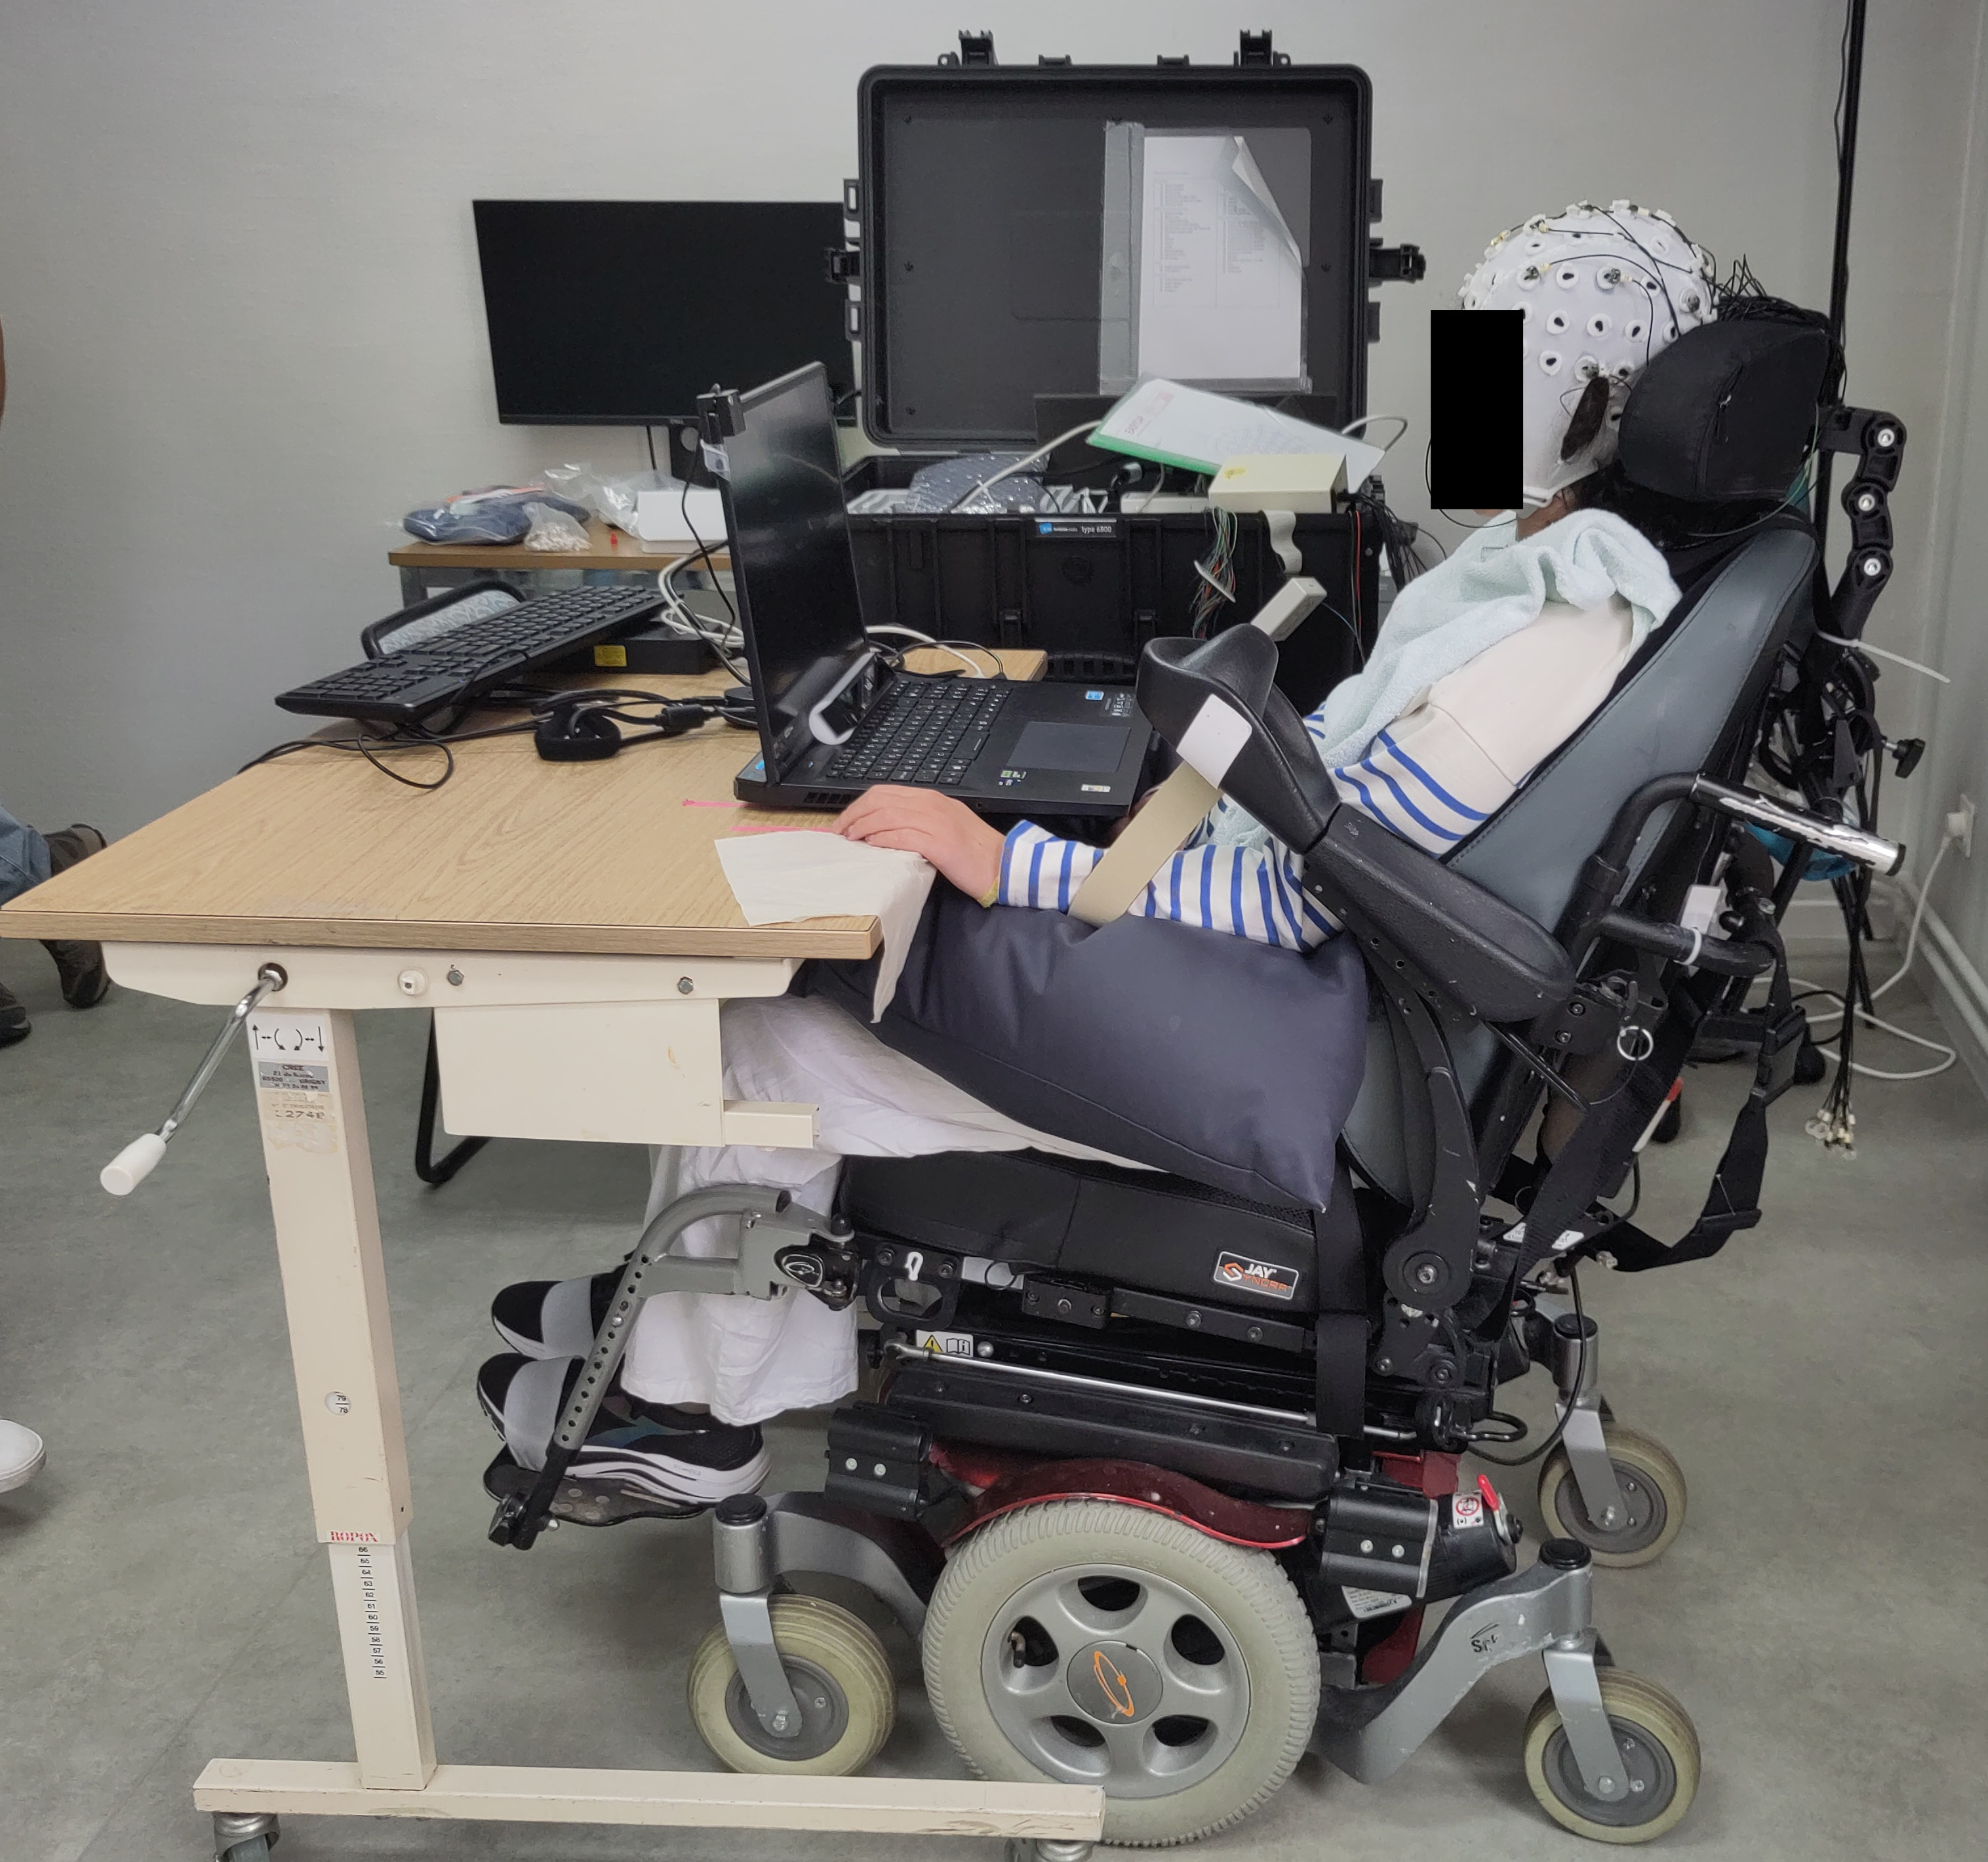
\includegraphics[width=\textwidth]{figures/PD01a-obfuscated.jpg}
  \end{minipage}\hfill%
  \begin{minipage}{.45\textwidth}
    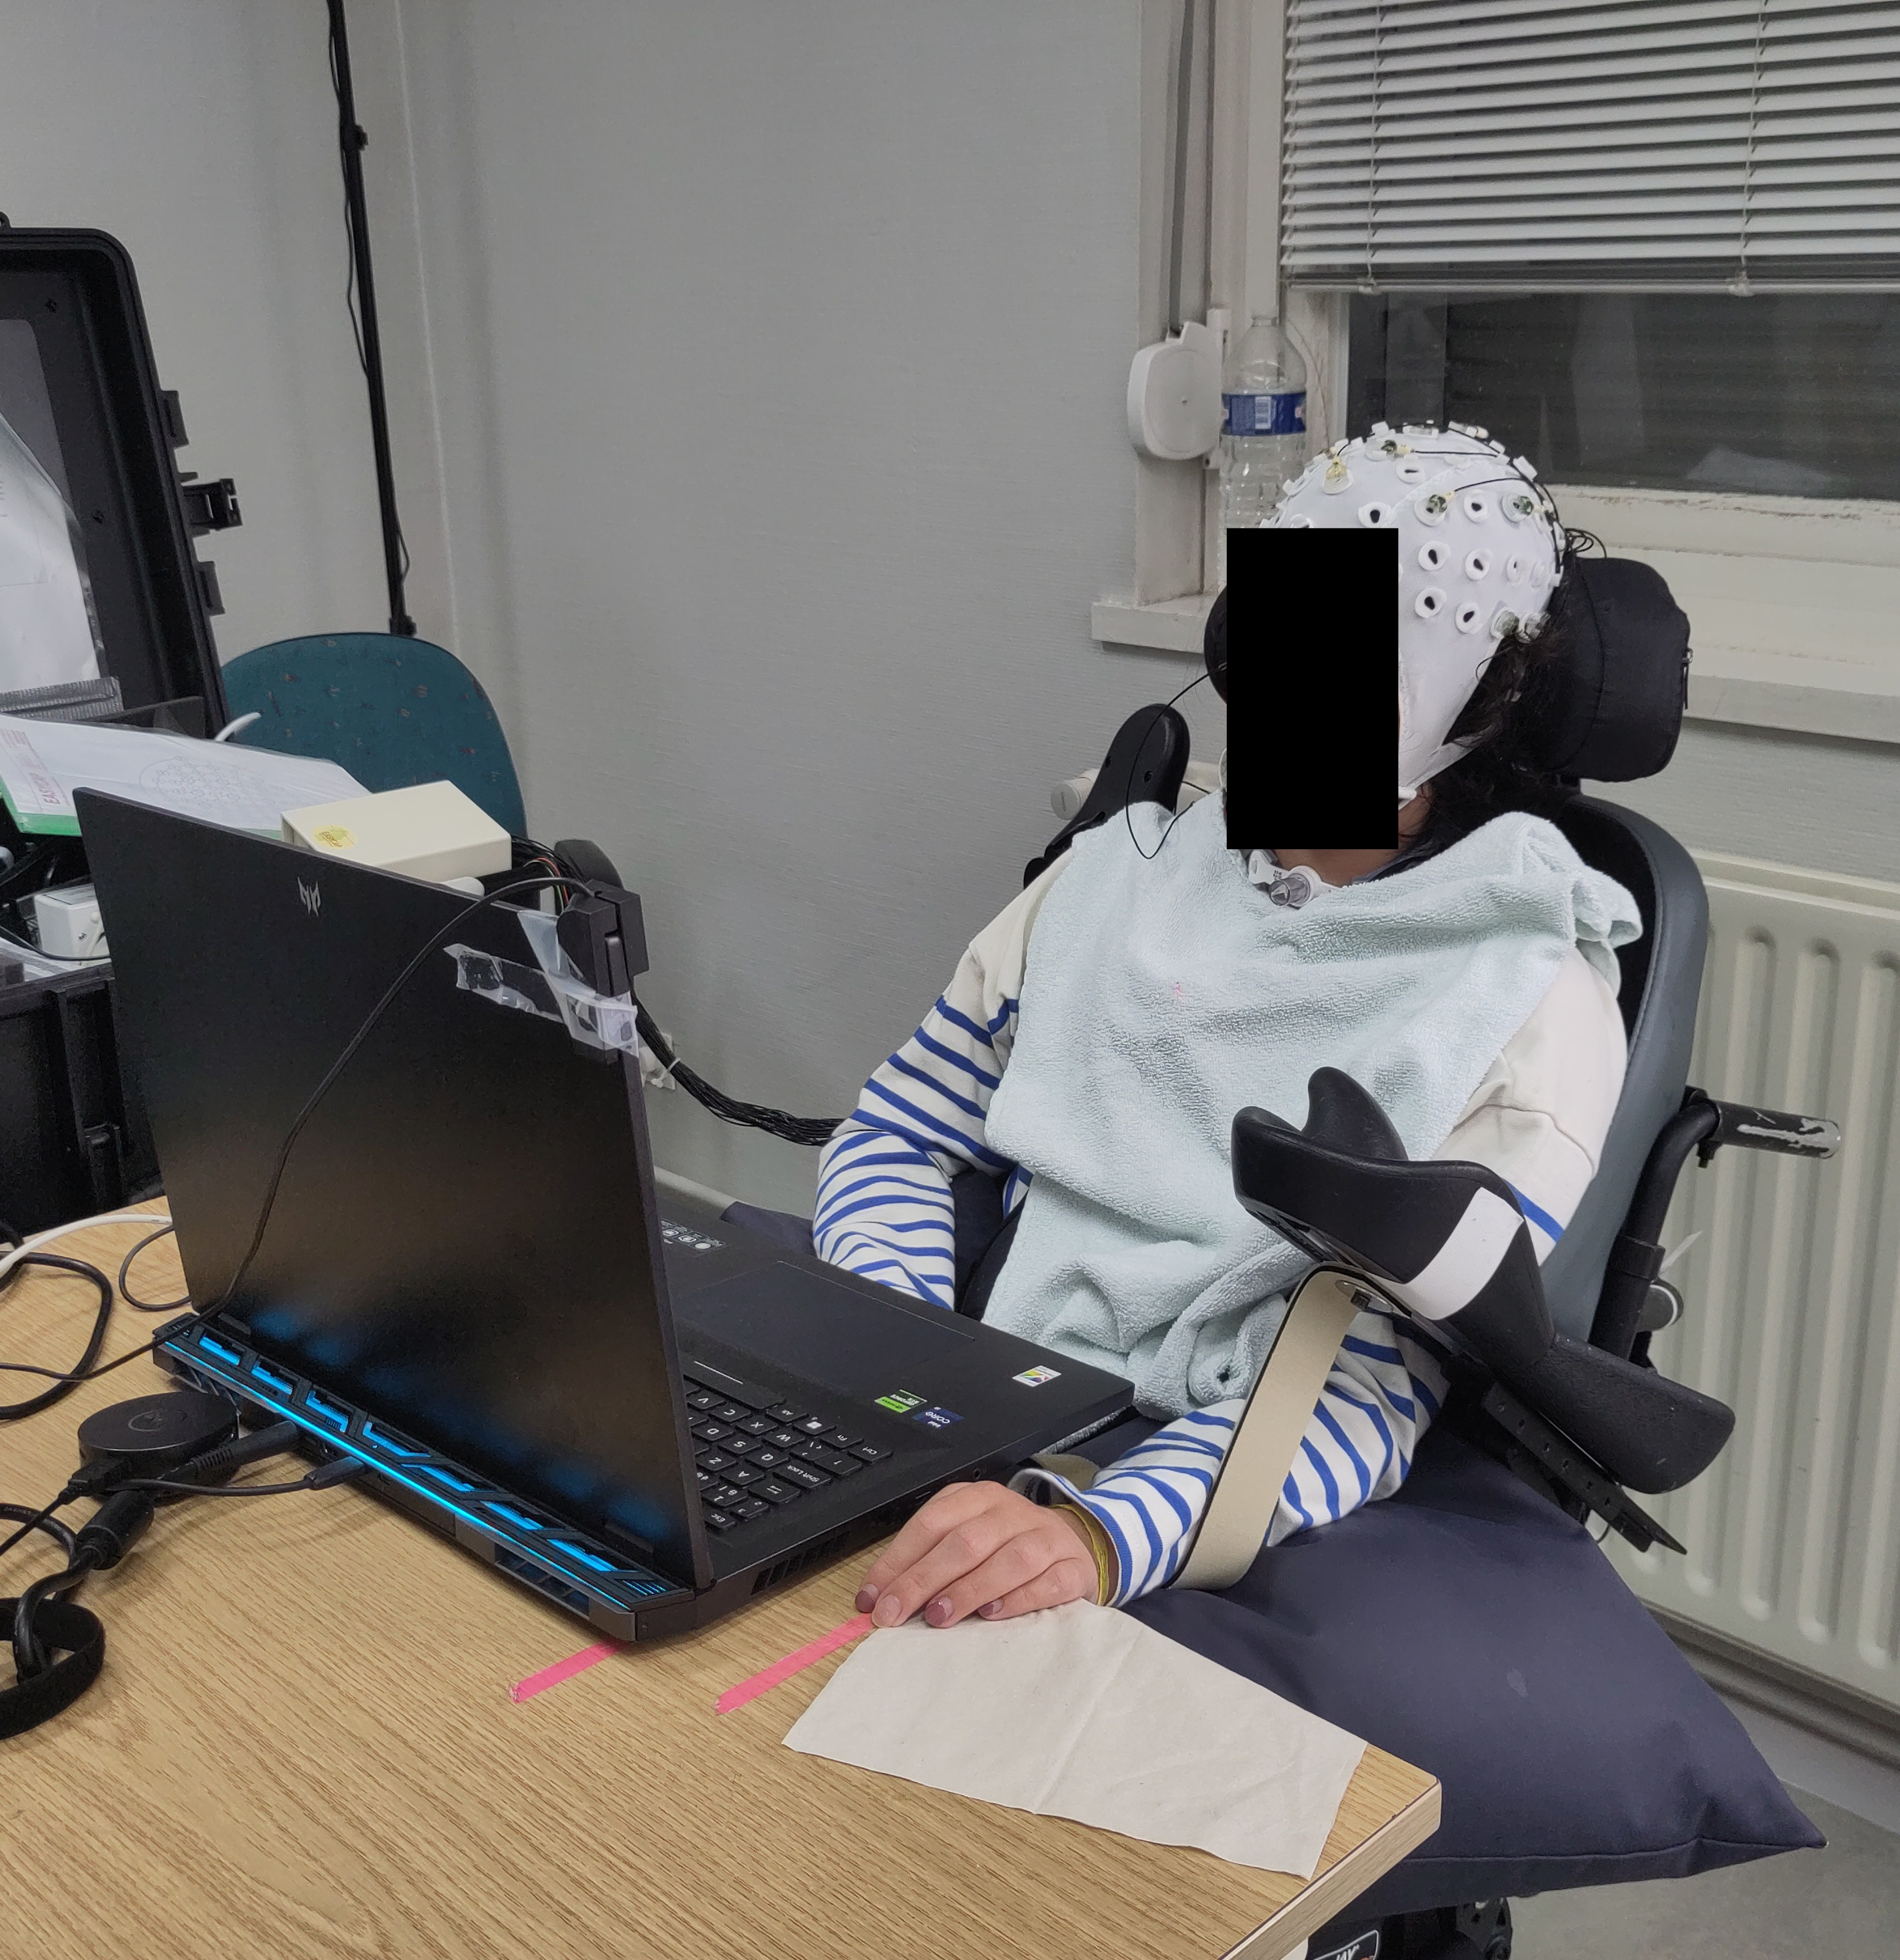
\includegraphics[width=\textwidth]{figures/PD01b-obfuscated.jpg}
  \end{minipage}
  \caption{A participant with the stimulation and recording setup.}
\end{figure*}

\subsection{Data collection \& preprocessing}

During the recording session, participants were positioned in their wheelchair in front of a table.
Stimuli were presented on an Acer Predator Helios laptop with an 18" screen (Acer,
Inc., Taiwan) placed at a 60 cm distance.
A Cedrus StimTracker (Cedrus Corp., CA, USA) ensured synchronization of stimuli with the
recorded \ac{eeg}.
Eye tracking was performed throughout using the Tobii X2-30 Compact (Tobii
Technology AB, Sweden) portable eye tracker placed at the bottom of the laptop screen.

\Ac{eeg} was recorded at 1000 Hz using the Neuroscan Neuvo portable amplifier (Compumedics Neuroscan,
Australia) connected to a second laptop for registration.
The \ac{eeg} headset used 18 active AgCl electrodes (EASYCAP GmbH, Germany) placed on a cap
according to the international 10-20 layout.
Using electrolyte gel, electrode impedances were reduced below 10 k$\Omega$.
Additionally, the \ac{eog} was recorded.

The \ac{eeg} was band-pass filtered between 0.5 and 16 Hz.
Bad channels were rejected using the RANSAC algorithm~\cite{Fischler1981}
and visual inspection.
Next, the \ac{eeg} was re-referenced to the average of mastoid electrodes TP9
and TP10, and \ac{ica} was performed to reject artifactual components based on
correlation with the \ac{eog} or by visual inspection.
Epochs were cut from -0.1 to 0.9 s relative to stimulus onset, and no baseline
correction was performed in order to meet the assumptions.

Eye tracking data was cleaned by fusing left and right gaze into one channel
for the horizontal and vertical gaze position.
If both were present for a given sample, the fused channel was the mean of both
values.
If at a given sample either the left or the right eye was not detected for a
given channel, the value of the other one was adopted.
If both were missing, the gaze position remained unset at that time point, and no
interpolation was performed of the employed classifiers.

\subsection{\Acs{bci} decoding}

We evaluated the recorded data using the \ac{wcble}~\cite{VanDenKerchove2024}
and \ac{tlda}~\cite{Sosulski2022}
classifiers, as well as the Riemannian approach XDAWNCov+TS+LDA~\cite{Cecotti2017}.
For \ac{wcble}, a region of interest from 0 ms to 800 ms relative to stimulus
onset was used while the epoch was cropped to -100 ms to 900 ms. For the other
decoders, the epoch was cropped between 0 ms and 800 ms, which resulted in maximal
performance.
Decoding scores were obtained using 6-fold cross-validation where folds corresponded to
stimulation blocks.

\section{Results}



\subsection{Visual skill and eye tracking analysis}
\label{sec:patients/outcomes/gaze}

Table~\ref{tab:patients/eye} details the eye motor impairments and vision of
the included participants.
All participants reported some degree of fatigue or discomfort when fixating.
Participant PA1 had the mildest impairment, only reporting fatigue when fixating
for prolonged times.
The \ac{fa} participants were mostly affected by eye tremors and impaired pursuit.
PB2 suffered from especially severe horizontal oscillating involuntary eye
movements.
Eye motor function of participants PC2, PC3, and PC4 was most severely affected.
Participant PC2 was only able to look up and down and had a deviation in the
left eye causing diplopia, but this was corrected by a prism glass.
Participant PC3 only retained partial motility of the right eye, while the left eye was permanently closed.
Participant PC4 had one deviated eye with a corneal abscess affecting the motility
and vision in the right eye, and reducing motility in the left.


Given these information, we aimed to shed more light on the actual capabilities of individuals
with \ac{sspgi} regarding performing overt \ac{vsa} and central gaze
fixation, as well as to investigate how relevant these two settings are when the
gaze is not cued.
\Cref{fig:patients/gaze} maps gaze position relative to the stimuli
across conditions.
These results should be interpreted with care, as the eye tracker to some
degree relies on functioning eye motility.
The participant's position relative to the eye tracker might have shifted
throughout the experimental session despite our best efforts, e.g., because they needed aspiration of their
tracheostomy.

\begin{figure*}
  %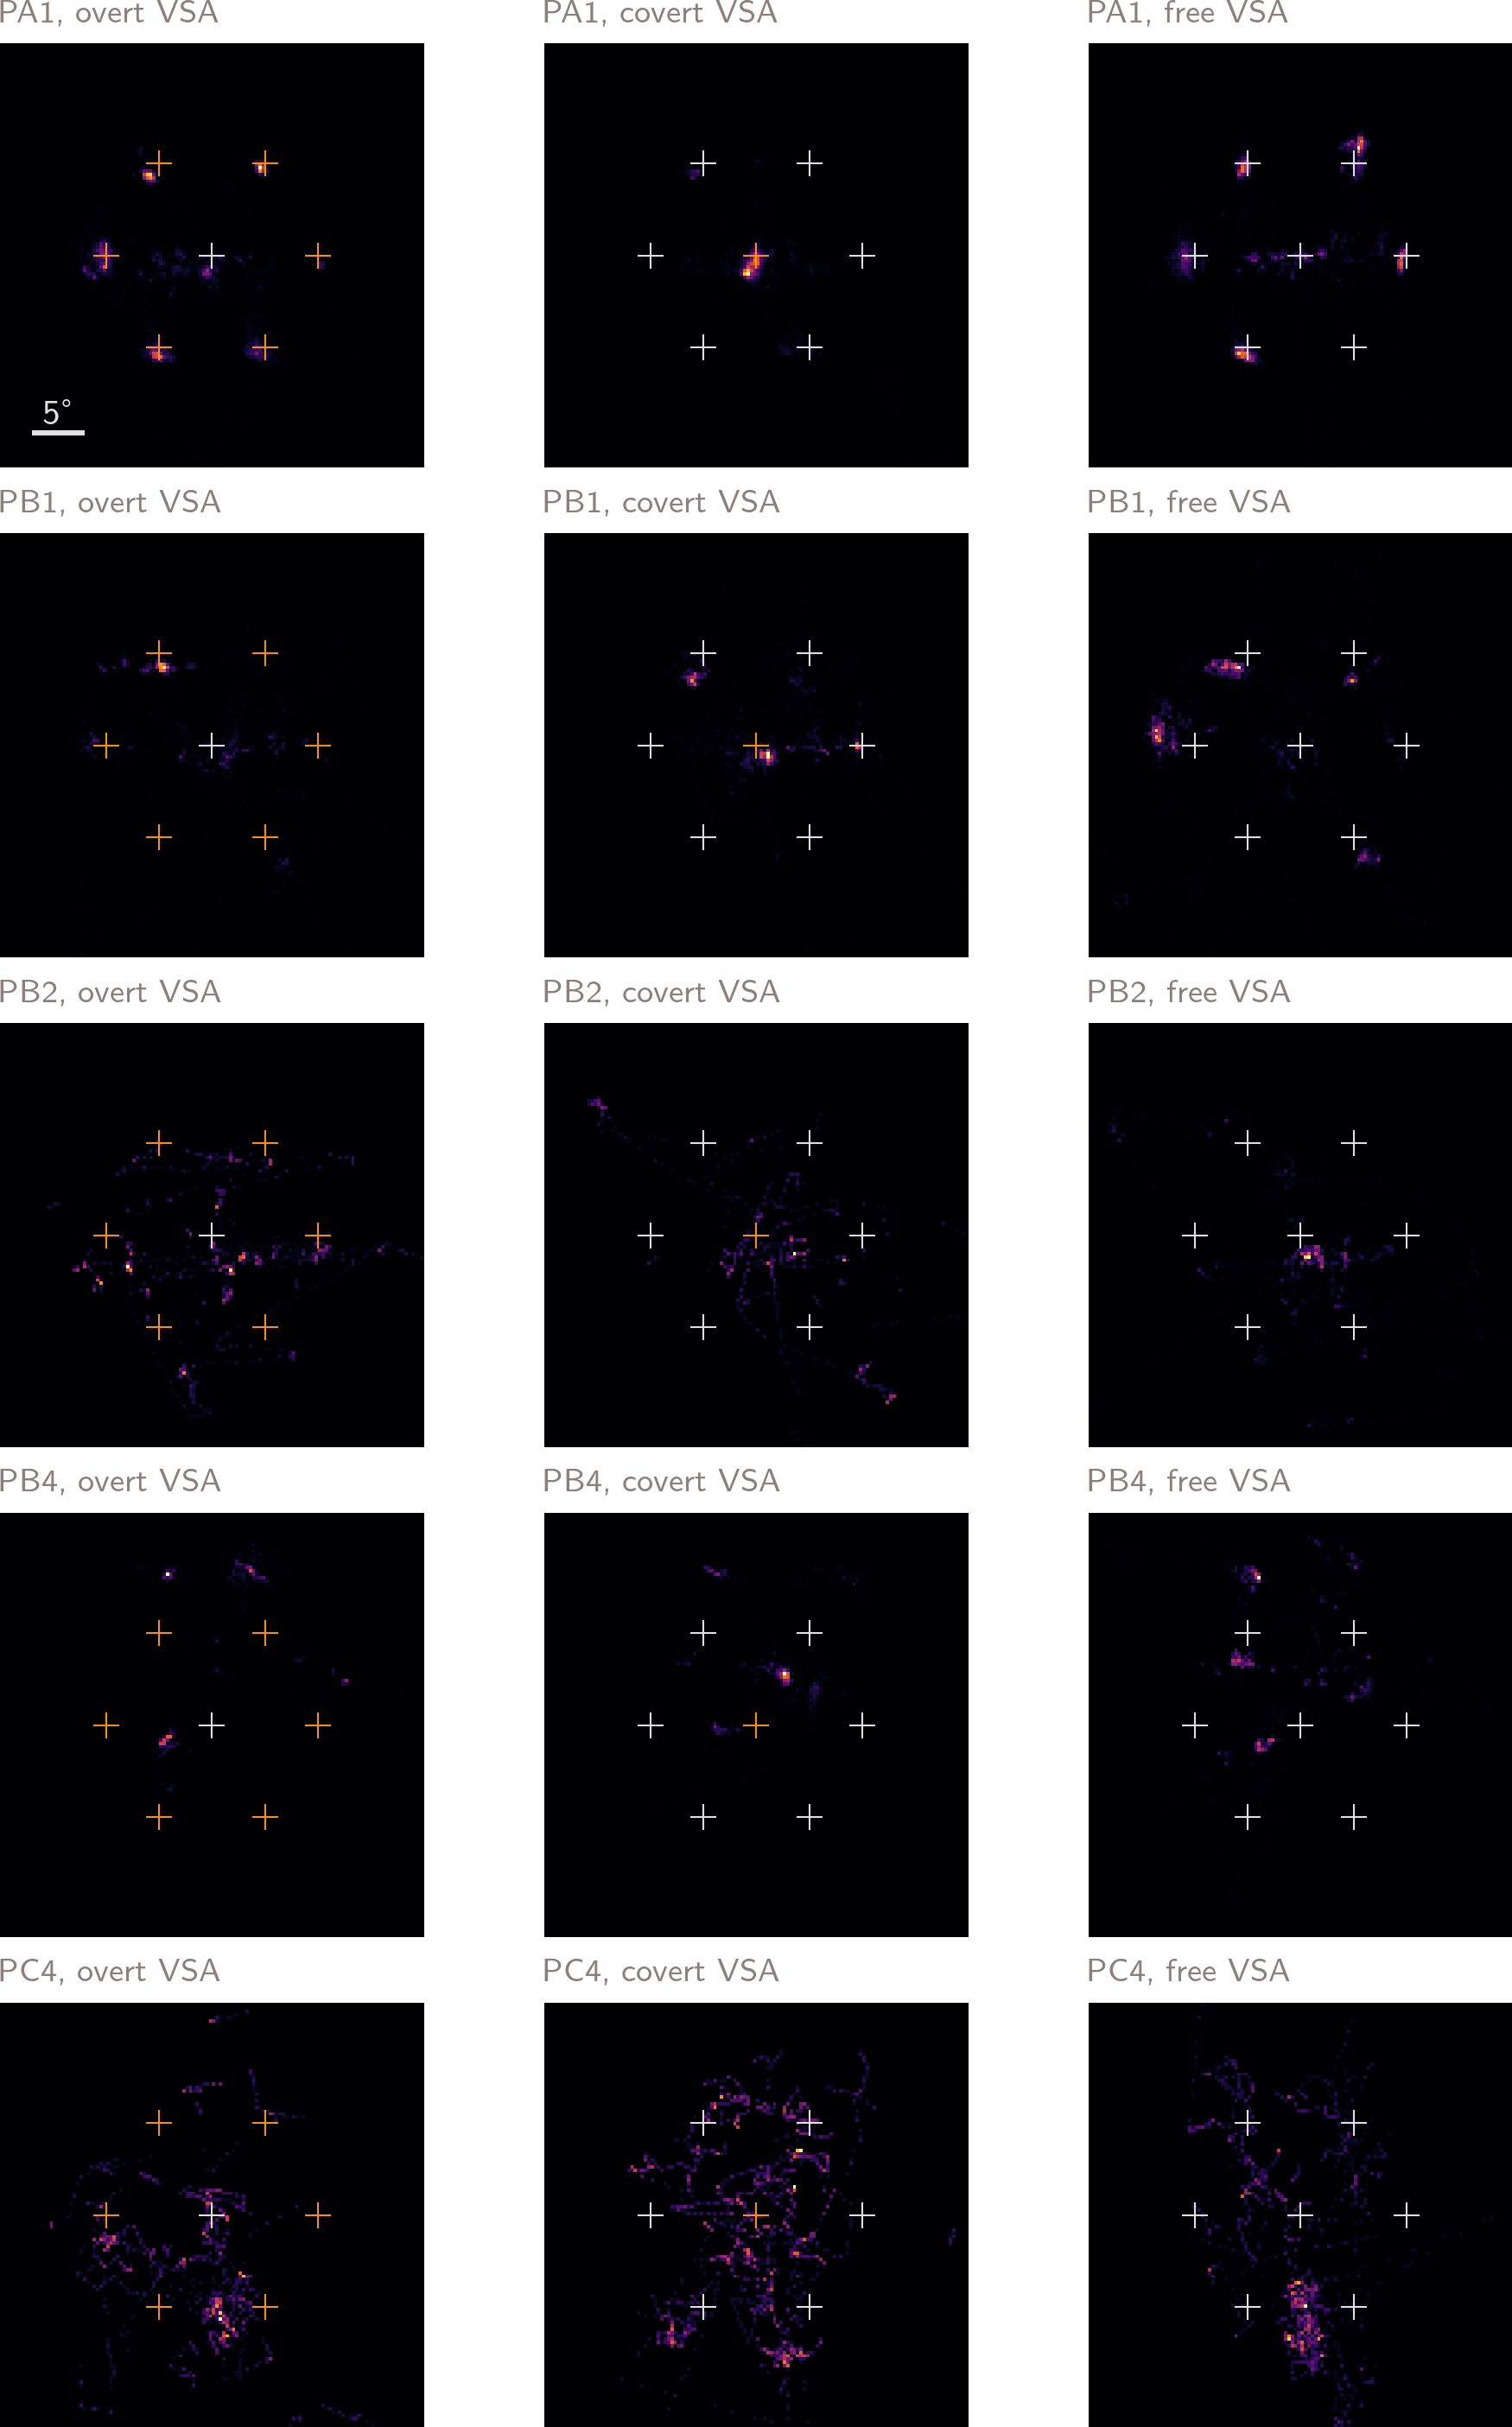
\includegraphics[width=\textwidth]{figures/fig_gaze.png}
  %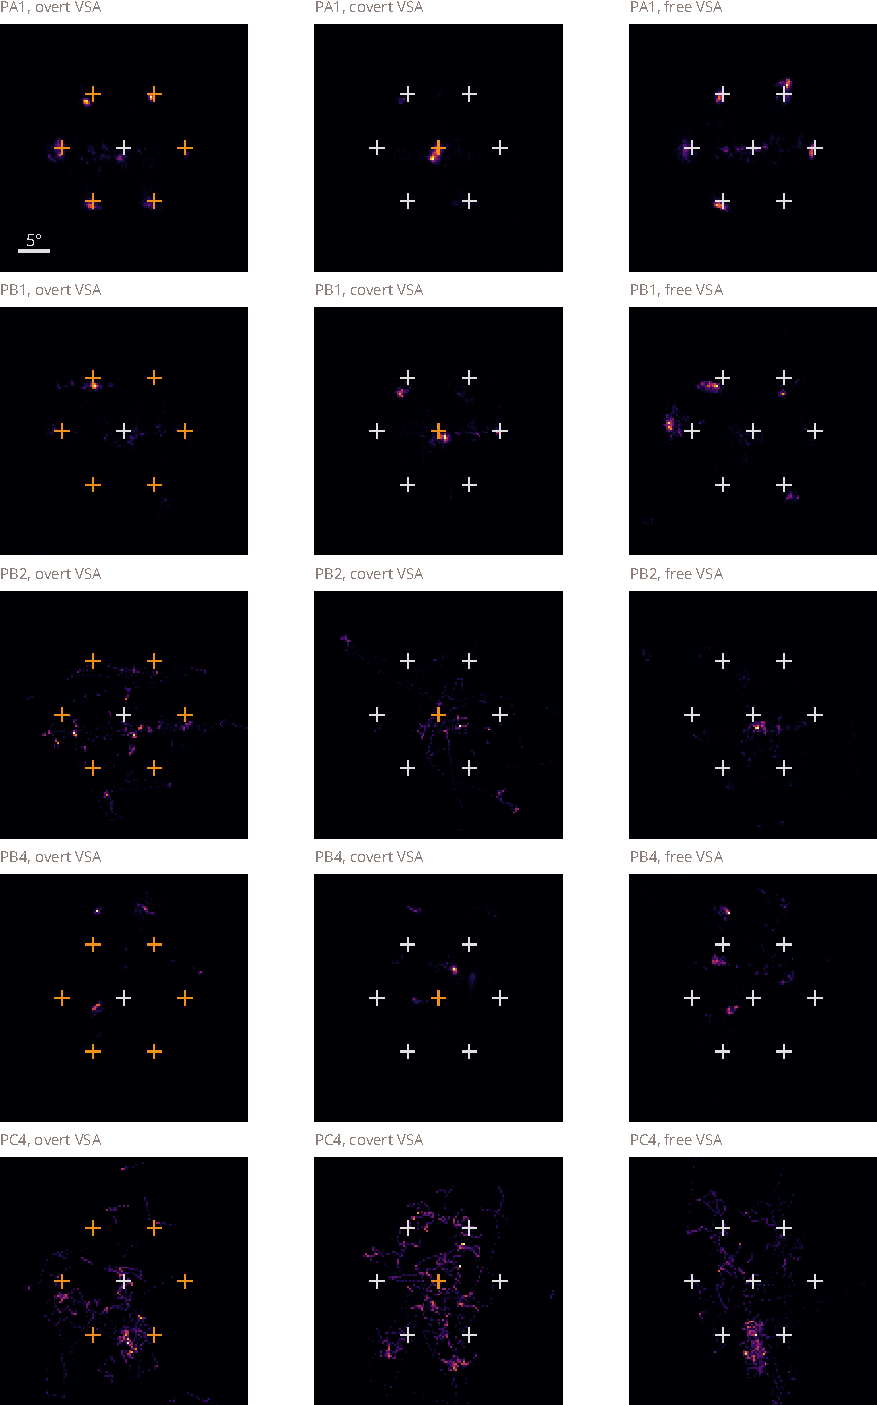
\includegraphics[width=\textwidth]{figures/fig_gaze.pdf}
  \pgfplotsset{%
    compat=newest,
    every axis/.append style={%
      every tick label style={color=lightgray},
      every axis label/.append style={color=lightgray},
      every title/.append style={color=lightgray},
      axis line style={color=lightgray}, % Set the axis line color to darkgray
    }
  }
  \import{figures}{fig_gaze.pgf}
  \caption[Distribution of the recorded gaze position.]{%
    Distribution of the recorded gaze position during the experimental session in the three \ac{vsa}
    conditions.
    Crosshairs represent stimulus positions, with the orange ones cued during
    the given condition.
    Subjects PB2 and PC4 preferred covert \ac{bci} operation, with PB2 resting gaze
    near the middle of the screen, and PC4 near the bottom.
  }
  \label{fig:patients/gaze}
\end{figure*}

PA1 had relatively intact gaze control and was able to correctly perform the
cued overt and covert settings.
When gaze was uncued, he fixated on the cued target.
This was also mostly the case for PB1, although eye tracking revealed that he
chose not to perform central gaze fixation when cued in at least one of the
stimulation blocks. We were unable to record his gaze near the bottom-left
stimulus position, either due to eye tracker failure or because the participant
was not comfortable fixating on this position.
Eye tracker calibration did not succeed for subject PB4, but given
transformation of gaze positions to the stimulus space, they were assumed to
be overtly performing the free task.

PB2 was able to perform overt \ac{vsa} and central fixation to some extent,
yet eye tracking shows a larger spread in gaze position compared to
PA1 and PB1.
In the free \ac{vsa} condition, however, she preferred to attend
stimuli covertly when the gaze was uncued.
This was confirmed by the participant.

The overt and central gaze fixation settings were also not properly adapted to
participant PC4.
In the free \ac{vsa} condition, eye tracker results show that his gaze was usually near the
bottom two targets, indicating some degree of covert or split \ac{vsa}.

It was technically impossible to register gaze position with the Tobii X2-30
Compact for participants PC2 and PC3 since they both had one eye that was
occluded respectively by the prism glass and the eyelid.
Both participants reported they could not fixate on some of the
stimuli.

\subsection{\Acs{bci} decoding performance}

\Cref{fig:patients/decode} shows single-trial
\ac{rocauc} in the evaluated \ac{vsa} settings for the different decoders.


In the overt \ac{vsa} setting, the evaluated decoders performed similarly on average
(\ac{wcble} 75.58\%, XDAWNCov+TS+LDA 74.24\%, \ac{tlda} 75.99\%).
In the covert \ac{vsa} setting with cued central gaze fixation, performance deteriorated,
but \ac{wcble} significantly improved performance over the base classifier
\ac{tlda} in this condition
(\ac{wcble} 62.49\%, XDAWNCov+TS+LDA 59.42\%, \ac{tlda} 59.05\%).
Decoding performance for this task was at chance level for participants PB4 and
PC3.

However, \ac{wcble} did not improve \ac{tlda} performance in the free \ac{vsa} setting, but
XDAWNCov+TS+LDA performance was slightly lower here (though not
significantly).
(\ac{wcble} 74.15\%, XDAWNCov+TS+LDA 71.88\%, \ac{tlda} 74.27\%).
More interestingly, we noticed that performances of the decoders in free
\ac{vsa} were close to those in the overt \ac{vsa}.
A substantial decrease in performance from the overt setting to the free
setting was observed for subjects PC3
(\ac{wcble}: 70.31>62.14 \%, XDAWNCov+TS+LDA: 65.78>62.18 \%, \ac{tlda}:
70.49>63.76 \%)
and PC4
(\ac{wcble}: 65.56>55.71 \%, XDAWNCov+TS+LDA: 62.02>54.24 \%, \ac{tlda}:
66.12>57.08 \%).
For PB2, who also relied on covert \ac{vsa} during the uncued free \ac{vsa}
according to gaze tracking setting, the decrease in performance was also
present, but not as substantial
(\ac{wcble}: 82.76>78.88 \%, XDAWNCov+TS+LDA: 80.74>77.99 \%, \ac{tlda}:
83.21>78.84 \%).

\begin{figure*}
  \hspace{-0.41662707185564984in}
%%% Creator: Matplotlib, PGF backend
%%
%% To include the figure in your LaTeX document, write
%%   \input{<filename>.pgf}
%%
%% Make sure the required packages are loaded in your preamble
%%   \usepackage{pgf}
%%
%% Also ensure that all the required font packages are loaded; for instance,
%% the lmodern package is sometimes necessary when using math font.
%%   \usepackage{lmodern}
%%
%% Figures using additional raster images can only be included by \input if
%% they are in the same directory as the main LaTeX file. For loading figures
%% from other directories you can use the `import` package
%%   \usepackage{import}
%%
%% and then include the figures with
%%   \import{<path to file>}{<filename>.pgf}
%%
%% Matplotlib used the following preamble
%%   \def\mathdefault#1{#1}
%%   \everymath=\expandafter{\the\everymath\displaystyle}
%%   
%%   \ifdefined\pdftexversion\else  % non-pdftex case.
%%     \usepackage{fontspec}
%%   \fi
%%   \makeatletter\@ifpackageloaded{underscore}{}{\usepackage[strings]{underscore}}\makeatother
%%
\begingroup%
\makeatletter%
\begin{pgfpicture}%
\pgfpathrectangle{\pgfpointorigin}{\pgfqpoint{5.057697in}{1.916660in}}%
\pgfusepath{use as bounding box, clip}%
\begin{pgfscope}%
\pgfsetbuttcap%
\pgfsetmiterjoin%
\pgfsetlinewidth{0.000000pt}%
\definecolor{currentstroke}{rgb}{1.000000,1.000000,1.000000}%
\pgfsetstrokecolor{currentstroke}%
\pgfsetstrokeopacity{0.000000}%
\pgfsetdash{}{0pt}%
\pgfpathmoveto{\pgfqpoint{0.000000in}{0.000000in}}%
\pgfpathlineto{\pgfqpoint{5.057697in}{0.000000in}}%
\pgfpathlineto{\pgfqpoint{5.057697in}{1.916660in}}%
\pgfpathlineto{\pgfqpoint{0.000000in}{1.916660in}}%
\pgfpathlineto{\pgfqpoint{0.000000in}{0.000000in}}%
\pgfpathclose%
\pgfusepath{}%
\end{pgfscope}%
\begin{pgfscope}%
\pgfsetbuttcap%
\pgfsetmiterjoin%
\definecolor{currentfill}{rgb}{1.000000,1.000000,1.000000}%
\pgfsetfillcolor{currentfill}%
\pgfsetlinewidth{0.000000pt}%
\definecolor{currentstroke}{rgb}{0.000000,0.000000,0.000000}%
\pgfsetstrokecolor{currentstroke}%
\pgfsetstrokeopacity{0.000000}%
\pgfsetdash{}{0pt}%
\pgfpathmoveto{\pgfqpoint{0.421874in}{0.447433in}}%
\pgfpathlineto{\pgfqpoint{1.911588in}{0.447433in}}%
\pgfpathlineto{\pgfqpoint{1.911588in}{1.746521in}}%
\pgfpathlineto{\pgfqpoint{0.421874in}{1.746521in}}%
\pgfpathlineto{\pgfqpoint{0.421874in}{0.447433in}}%
\pgfpathclose%
\pgfusepath{fill}%
\end{pgfscope}%
\begin{pgfscope}%
\pgfpathrectangle{\pgfqpoint{0.421874in}{0.447433in}}{\pgfqpoint{1.489714in}{1.299088in}}%
\pgfusepath{clip}%
\pgfsetbuttcap%
\pgfsetmiterjoin%
\definecolor{currentfill}{rgb}{0.842157,0.553922,0.200980}%
\pgfsetfillcolor{currentfill}%
\pgfsetlinewidth{0.000000pt}%
\definecolor{currentstroke}{rgb}{0.000000,0.000000,0.000000}%
\pgfsetstrokecolor{currentstroke}%
\pgfsetstrokeopacity{0.000000}%
\pgfsetdash{}{0pt}%
\pgfpathmoveto{\pgfqpoint{0.440495in}{0.447433in}}%
\pgfpathlineto{\pgfqpoint{0.490152in}{0.447433in}}%
\pgfpathlineto{\pgfqpoint{0.490152in}{1.318527in}}%
\pgfpathlineto{\pgfqpoint{0.440495in}{1.318527in}}%
\pgfpathlineto{\pgfqpoint{0.440495in}{0.447433in}}%
\pgfpathclose%
\pgfusepath{fill}%
\end{pgfscope}%
\begin{pgfscope}%
\pgfpathrectangle{\pgfqpoint{0.421874in}{0.447433in}}{\pgfqpoint{1.489714in}{1.299088in}}%
\pgfusepath{clip}%
\pgfsetbuttcap%
\pgfsetmiterjoin%
\definecolor{currentfill}{rgb}{0.842157,0.553922,0.200980}%
\pgfsetfillcolor{currentfill}%
\pgfsetlinewidth{0.000000pt}%
\definecolor{currentstroke}{rgb}{0.000000,0.000000,0.000000}%
\pgfsetstrokecolor{currentstroke}%
\pgfsetstrokeopacity{0.000000}%
\pgfsetdash{}{0pt}%
\pgfpathmoveto{\pgfqpoint{0.626709in}{0.447433in}}%
\pgfpathlineto{\pgfqpoint{0.676367in}{0.447433in}}%
\pgfpathlineto{\pgfqpoint{0.676367in}{1.627122in}}%
\pgfpathlineto{\pgfqpoint{0.626709in}{1.627122in}}%
\pgfpathlineto{\pgfqpoint{0.626709in}{0.447433in}}%
\pgfpathclose%
\pgfusepath{fill}%
\end{pgfscope}%
\begin{pgfscope}%
\pgfpathrectangle{\pgfqpoint{0.421874in}{0.447433in}}{\pgfqpoint{1.489714in}{1.299088in}}%
\pgfusepath{clip}%
\pgfsetbuttcap%
\pgfsetmiterjoin%
\definecolor{currentfill}{rgb}{0.842157,0.553922,0.200980}%
\pgfsetfillcolor{currentfill}%
\pgfsetlinewidth{0.000000pt}%
\definecolor{currentstroke}{rgb}{0.000000,0.000000,0.000000}%
\pgfsetstrokecolor{currentstroke}%
\pgfsetstrokeopacity{0.000000}%
\pgfsetdash{}{0pt}%
\pgfpathmoveto{\pgfqpoint{0.812924in}{0.447433in}}%
\pgfpathlineto{\pgfqpoint{0.862581in}{0.447433in}}%
\pgfpathlineto{\pgfqpoint{0.862581in}{1.528425in}}%
\pgfpathlineto{\pgfqpoint{0.812924in}{1.528425in}}%
\pgfpathlineto{\pgfqpoint{0.812924in}{0.447433in}}%
\pgfpathclose%
\pgfusepath{fill}%
\end{pgfscope}%
\begin{pgfscope}%
\pgfpathrectangle{\pgfqpoint{0.421874in}{0.447433in}}{\pgfqpoint{1.489714in}{1.299088in}}%
\pgfusepath{clip}%
\pgfsetbuttcap%
\pgfsetmiterjoin%
\definecolor{currentfill}{rgb}{0.842157,0.553922,0.200980}%
\pgfsetfillcolor{currentfill}%
\pgfsetlinewidth{0.000000pt}%
\definecolor{currentstroke}{rgb}{0.000000,0.000000,0.000000}%
\pgfsetstrokecolor{currentstroke}%
\pgfsetstrokeopacity{0.000000}%
\pgfsetdash{}{0pt}%
\pgfpathmoveto{\pgfqpoint{0.999138in}{0.447433in}}%
\pgfpathlineto{\pgfqpoint{1.048795in}{0.447433in}}%
\pgfpathlineto{\pgfqpoint{1.048795in}{1.528136in}}%
\pgfpathlineto{\pgfqpoint{0.999138in}{1.528136in}}%
\pgfpathlineto{\pgfqpoint{0.999138in}{0.447433in}}%
\pgfpathclose%
\pgfusepath{fill}%
\end{pgfscope}%
\begin{pgfscope}%
\pgfpathrectangle{\pgfqpoint{0.421874in}{0.447433in}}{\pgfqpoint{1.489714in}{1.299088in}}%
\pgfusepath{clip}%
\pgfsetbuttcap%
\pgfsetmiterjoin%
\definecolor{currentfill}{rgb}{0.842157,0.553922,0.200980}%
\pgfsetfillcolor{currentfill}%
\pgfsetlinewidth{0.000000pt}%
\definecolor{currentstroke}{rgb}{0.000000,0.000000,0.000000}%
\pgfsetstrokecolor{currentstroke}%
\pgfsetstrokeopacity{0.000000}%
\pgfsetdash{}{0pt}%
\pgfpathmoveto{\pgfqpoint{1.185352in}{0.447433in}}%
\pgfpathlineto{\pgfqpoint{1.235009in}{0.447433in}}%
\pgfpathlineto{\pgfqpoint{1.235009in}{1.370255in}}%
\pgfpathlineto{\pgfqpoint{1.185352in}{1.370255in}}%
\pgfpathlineto{\pgfqpoint{1.185352in}{0.447433in}}%
\pgfpathclose%
\pgfusepath{fill}%
\end{pgfscope}%
\begin{pgfscope}%
\pgfpathrectangle{\pgfqpoint{0.421874in}{0.447433in}}{\pgfqpoint{1.489714in}{1.299088in}}%
\pgfusepath{clip}%
\pgfsetbuttcap%
\pgfsetmiterjoin%
\definecolor{currentfill}{rgb}{0.842157,0.553922,0.200980}%
\pgfsetfillcolor{currentfill}%
\pgfsetlinewidth{0.000000pt}%
\definecolor{currentstroke}{rgb}{0.000000,0.000000,0.000000}%
\pgfsetstrokecolor{currentstroke}%
\pgfsetstrokeopacity{0.000000}%
\pgfsetdash{}{0pt}%
\pgfpathmoveto{\pgfqpoint{1.371567in}{0.447433in}}%
\pgfpathlineto{\pgfqpoint{1.421224in}{0.447433in}}%
\pgfpathlineto{\pgfqpoint{1.421224in}{1.363222in}}%
\pgfpathlineto{\pgfqpoint{1.371567in}{1.363222in}}%
\pgfpathlineto{\pgfqpoint{1.371567in}{0.447433in}}%
\pgfpathclose%
\pgfusepath{fill}%
\end{pgfscope}%
\begin{pgfscope}%
\pgfpathrectangle{\pgfqpoint{0.421874in}{0.447433in}}{\pgfqpoint{1.489714in}{1.299088in}}%
\pgfusepath{clip}%
\pgfsetbuttcap%
\pgfsetmiterjoin%
\definecolor{currentfill}{rgb}{0.842157,0.553922,0.200980}%
\pgfsetfillcolor{currentfill}%
\pgfsetlinewidth{0.000000pt}%
\definecolor{currentstroke}{rgb}{0.000000,0.000000,0.000000}%
\pgfsetstrokecolor{currentstroke}%
\pgfsetstrokeopacity{0.000000}%
\pgfsetdash{}{0pt}%
\pgfpathmoveto{\pgfqpoint{1.557781in}{0.447433in}}%
\pgfpathlineto{\pgfqpoint{1.607438in}{0.447433in}}%
\pgfpathlineto{\pgfqpoint{1.607438in}{1.306366in}}%
\pgfpathlineto{\pgfqpoint{1.557781in}{1.306366in}}%
\pgfpathlineto{\pgfqpoint{1.557781in}{0.447433in}}%
\pgfpathclose%
\pgfusepath{fill}%
\end{pgfscope}%
\begin{pgfscope}%
\pgfpathrectangle{\pgfqpoint{0.421874in}{0.447433in}}{\pgfqpoint{1.489714in}{1.299088in}}%
\pgfusepath{clip}%
\pgfsetbuttcap%
\pgfsetmiterjoin%
\definecolor{currentfill}{rgb}{0.842157,0.553922,0.200980}%
\pgfsetfillcolor{currentfill}%
\pgfsetlinewidth{0.000000pt}%
\definecolor{currentstroke}{rgb}{0.000000,0.000000,0.000000}%
\pgfsetstrokecolor{currentstroke}%
\pgfsetstrokeopacity{0.000000}%
\pgfsetdash{}{0pt}%
\pgfpathmoveto{\pgfqpoint{1.743995in}{0.447433in}}%
\pgfpathlineto{\pgfqpoint{1.793652in}{0.447433in}}%
\pgfpathlineto{\pgfqpoint{1.793652in}{1.434579in}}%
\pgfpathlineto{\pgfqpoint{1.743995in}{1.434579in}}%
\pgfpathlineto{\pgfqpoint{1.743995in}{0.447433in}}%
\pgfpathclose%
\pgfusepath{fill}%
\end{pgfscope}%
\begin{pgfscope}%
\pgfpathrectangle{\pgfqpoint{0.421874in}{0.447433in}}{\pgfqpoint{1.489714in}{1.299088in}}%
\pgfusepath{clip}%
\pgfsetbuttcap%
\pgfsetmiterjoin%
\definecolor{currentfill}{rgb}{0.858824,0.314706,0.223529}%
\pgfsetfillcolor{currentfill}%
\pgfsetlinewidth{0.000000pt}%
\definecolor{currentstroke}{rgb}{0.000000,0.000000,0.000000}%
\pgfsetstrokecolor{currentstroke}%
\pgfsetstrokeopacity{0.000000}%
\pgfsetdash{}{0pt}%
\pgfpathmoveto{\pgfqpoint{0.490152in}{0.447433in}}%
\pgfpathlineto{\pgfqpoint{0.539809in}{0.447433in}}%
\pgfpathlineto{\pgfqpoint{0.539809in}{1.376937in}}%
\pgfpathlineto{\pgfqpoint{0.490152in}{1.376937in}}%
\pgfpathlineto{\pgfqpoint{0.490152in}{0.447433in}}%
\pgfpathclose%
\pgfusepath{fill}%
\end{pgfscope}%
\begin{pgfscope}%
\pgfpathrectangle{\pgfqpoint{0.421874in}{0.447433in}}{\pgfqpoint{1.489714in}{1.299088in}}%
\pgfusepath{clip}%
\pgfsetbuttcap%
\pgfsetmiterjoin%
\definecolor{currentfill}{rgb}{0.858824,0.314706,0.223529}%
\pgfsetfillcolor{currentfill}%
\pgfsetlinewidth{0.000000pt}%
\definecolor{currentstroke}{rgb}{0.000000,0.000000,0.000000}%
\pgfsetstrokecolor{currentstroke}%
\pgfsetstrokeopacity{0.000000}%
\pgfsetdash{}{0pt}%
\pgfpathmoveto{\pgfqpoint{0.676367in}{0.447433in}}%
\pgfpathlineto{\pgfqpoint{0.726024in}{0.447433in}}%
\pgfpathlineto{\pgfqpoint{0.726024in}{1.609971in}}%
\pgfpathlineto{\pgfqpoint{0.676367in}{1.609971in}}%
\pgfpathlineto{\pgfqpoint{0.676367in}{0.447433in}}%
\pgfpathclose%
\pgfusepath{fill}%
\end{pgfscope}%
\begin{pgfscope}%
\pgfpathrectangle{\pgfqpoint{0.421874in}{0.447433in}}{\pgfqpoint{1.489714in}{1.299088in}}%
\pgfusepath{clip}%
\pgfsetbuttcap%
\pgfsetmiterjoin%
\definecolor{currentfill}{rgb}{0.858824,0.314706,0.223529}%
\pgfsetfillcolor{currentfill}%
\pgfsetlinewidth{0.000000pt}%
\definecolor{currentstroke}{rgb}{0.000000,0.000000,0.000000}%
\pgfsetstrokecolor{currentstroke}%
\pgfsetstrokeopacity{0.000000}%
\pgfsetdash{}{0pt}%
\pgfpathmoveto{\pgfqpoint{0.862581in}{0.447433in}}%
\pgfpathlineto{\pgfqpoint{0.912238in}{0.447433in}}%
\pgfpathlineto{\pgfqpoint{0.912238in}{1.522529in}}%
\pgfpathlineto{\pgfqpoint{0.862581in}{1.522529in}}%
\pgfpathlineto{\pgfqpoint{0.862581in}{0.447433in}}%
\pgfpathclose%
\pgfusepath{fill}%
\end{pgfscope}%
\begin{pgfscope}%
\pgfpathrectangle{\pgfqpoint{0.421874in}{0.447433in}}{\pgfqpoint{1.489714in}{1.299088in}}%
\pgfusepath{clip}%
\pgfsetbuttcap%
\pgfsetmiterjoin%
\definecolor{currentfill}{rgb}{0.858824,0.314706,0.223529}%
\pgfsetfillcolor{currentfill}%
\pgfsetlinewidth{0.000000pt}%
\definecolor{currentstroke}{rgb}{0.000000,0.000000,0.000000}%
\pgfsetstrokecolor{currentstroke}%
\pgfsetstrokeopacity{0.000000}%
\pgfsetdash{}{0pt}%
\pgfpathmoveto{\pgfqpoint{1.048795in}{0.447433in}}%
\pgfpathlineto{\pgfqpoint{1.098452in}{0.447433in}}%
\pgfpathlineto{\pgfqpoint{1.098452in}{1.493636in}}%
\pgfpathlineto{\pgfqpoint{1.048795in}{1.493636in}}%
\pgfpathlineto{\pgfqpoint{1.048795in}{0.447433in}}%
\pgfpathclose%
\pgfusepath{fill}%
\end{pgfscope}%
\begin{pgfscope}%
\pgfpathrectangle{\pgfqpoint{0.421874in}{0.447433in}}{\pgfqpoint{1.489714in}{1.299088in}}%
\pgfusepath{clip}%
\pgfsetbuttcap%
\pgfsetmiterjoin%
\definecolor{currentfill}{rgb}{0.858824,0.314706,0.223529}%
\pgfsetfillcolor{currentfill}%
\pgfsetlinewidth{0.000000pt}%
\definecolor{currentstroke}{rgb}{0.000000,0.000000,0.000000}%
\pgfsetstrokecolor{currentstroke}%
\pgfsetstrokeopacity{0.000000}%
\pgfsetdash{}{0pt}%
\pgfpathmoveto{\pgfqpoint{1.235009in}{0.447433in}}%
\pgfpathlineto{\pgfqpoint{1.284667in}{0.447433in}}%
\pgfpathlineto{\pgfqpoint{1.284667in}{1.340816in}}%
\pgfpathlineto{\pgfqpoint{1.235009in}{1.340816in}}%
\pgfpathlineto{\pgfqpoint{1.235009in}{0.447433in}}%
\pgfpathclose%
\pgfusepath{fill}%
\end{pgfscope}%
\begin{pgfscope}%
\pgfpathrectangle{\pgfqpoint{0.421874in}{0.447433in}}{\pgfqpoint{1.489714in}{1.299088in}}%
\pgfusepath{clip}%
\pgfsetbuttcap%
\pgfsetmiterjoin%
\definecolor{currentfill}{rgb}{0.858824,0.314706,0.223529}%
\pgfsetfillcolor{currentfill}%
\pgfsetlinewidth{0.000000pt}%
\definecolor{currentstroke}{rgb}{0.000000,0.000000,0.000000}%
\pgfsetstrokecolor{currentstroke}%
\pgfsetstrokeopacity{0.000000}%
\pgfsetdash{}{0pt}%
\pgfpathmoveto{\pgfqpoint{1.421224in}{0.447433in}}%
\pgfpathlineto{\pgfqpoint{1.470881in}{0.447433in}}%
\pgfpathlineto{\pgfqpoint{1.470881in}{1.360833in}}%
\pgfpathlineto{\pgfqpoint{1.421224in}{1.360833in}}%
\pgfpathlineto{\pgfqpoint{1.421224in}{0.447433in}}%
\pgfpathclose%
\pgfusepath{fill}%
\end{pgfscope}%
\begin{pgfscope}%
\pgfpathrectangle{\pgfqpoint{0.421874in}{0.447433in}}{\pgfqpoint{1.489714in}{1.299088in}}%
\pgfusepath{clip}%
\pgfsetbuttcap%
\pgfsetmiterjoin%
\definecolor{currentfill}{rgb}{0.858824,0.314706,0.223529}%
\pgfsetfillcolor{currentfill}%
\pgfsetlinewidth{0.000000pt}%
\definecolor{currentstroke}{rgb}{0.000000,0.000000,0.000000}%
\pgfsetstrokecolor{currentstroke}%
\pgfsetstrokeopacity{0.000000}%
\pgfsetdash{}{0pt}%
\pgfpathmoveto{\pgfqpoint{1.607438in}{0.447433in}}%
\pgfpathlineto{\pgfqpoint{1.657095in}{0.447433in}}%
\pgfpathlineto{\pgfqpoint{1.657095in}{1.300286in}}%
\pgfpathlineto{\pgfqpoint{1.607438in}{1.300286in}}%
\pgfpathlineto{\pgfqpoint{1.607438in}{0.447433in}}%
\pgfpathclose%
\pgfusepath{fill}%
\end{pgfscope}%
\begin{pgfscope}%
\pgfpathrectangle{\pgfqpoint{0.421874in}{0.447433in}}{\pgfqpoint{1.489714in}{1.299088in}}%
\pgfusepath{clip}%
\pgfsetbuttcap%
\pgfsetmiterjoin%
\definecolor{currentfill}{rgb}{0.858824,0.314706,0.223529}%
\pgfsetfillcolor{currentfill}%
\pgfsetlinewidth{0.000000pt}%
\definecolor{currentstroke}{rgb}{0.000000,0.000000,0.000000}%
\pgfsetstrokecolor{currentstroke}%
\pgfsetstrokeopacity{0.000000}%
\pgfsetdash{}{0pt}%
\pgfpathmoveto{\pgfqpoint{1.793652in}{0.447433in}}%
\pgfpathlineto{\pgfqpoint{1.843309in}{0.447433in}}%
\pgfpathlineto{\pgfqpoint{1.843309in}{1.429287in}}%
\pgfpathlineto{\pgfqpoint{1.793652in}{1.429287in}}%
\pgfpathlineto{\pgfqpoint{1.793652in}{0.447433in}}%
\pgfpathclose%
\pgfusepath{fill}%
\end{pgfscope}%
\begin{pgfscope}%
\pgfpathrectangle{\pgfqpoint{0.421874in}{0.447433in}}{\pgfqpoint{1.489714in}{1.299088in}}%
\pgfusepath{clip}%
\pgfsetbuttcap%
\pgfsetmiterjoin%
\definecolor{currentfill}{rgb}{0.464706,0.320588,0.573529}%
\pgfsetfillcolor{currentfill}%
\pgfsetlinewidth{0.000000pt}%
\definecolor{currentstroke}{rgb}{0.000000,0.000000,0.000000}%
\pgfsetstrokecolor{currentstroke}%
\pgfsetstrokeopacity{0.000000}%
\pgfsetdash{}{0pt}%
\pgfpathmoveto{\pgfqpoint{0.539809in}{0.447433in}}%
\pgfpathlineto{\pgfqpoint{0.589467in}{0.447433in}}%
\pgfpathlineto{\pgfqpoint{0.589467in}{1.329460in}}%
\pgfpathlineto{\pgfqpoint{0.539809in}{1.329460in}}%
\pgfpathlineto{\pgfqpoint{0.539809in}{0.447433in}}%
\pgfpathclose%
\pgfusepath{fill}%
\end{pgfscope}%
\begin{pgfscope}%
\pgfpathrectangle{\pgfqpoint{0.421874in}{0.447433in}}{\pgfqpoint{1.489714in}{1.299088in}}%
\pgfusepath{clip}%
\pgfsetbuttcap%
\pgfsetmiterjoin%
\definecolor{currentfill}{rgb}{0.464706,0.320588,0.573529}%
\pgfsetfillcolor{currentfill}%
\pgfsetlinewidth{0.000000pt}%
\definecolor{currentstroke}{rgb}{0.000000,0.000000,0.000000}%
\pgfsetstrokecolor{currentstroke}%
\pgfsetstrokeopacity{0.000000}%
\pgfsetdash{}{0pt}%
\pgfpathmoveto{\pgfqpoint{0.726024in}{0.447433in}}%
\pgfpathlineto{\pgfqpoint{0.775681in}{0.447433in}}%
\pgfpathlineto{\pgfqpoint{0.775681in}{1.611034in}}%
\pgfpathlineto{\pgfqpoint{0.726024in}{1.611034in}}%
\pgfpathlineto{\pgfqpoint{0.726024in}{0.447433in}}%
\pgfpathclose%
\pgfusepath{fill}%
\end{pgfscope}%
\begin{pgfscope}%
\pgfpathrectangle{\pgfqpoint{0.421874in}{0.447433in}}{\pgfqpoint{1.489714in}{1.299088in}}%
\pgfusepath{clip}%
\pgfsetbuttcap%
\pgfsetmiterjoin%
\definecolor{currentfill}{rgb}{0.464706,0.320588,0.573529}%
\pgfsetfillcolor{currentfill}%
\pgfsetlinewidth{0.000000pt}%
\definecolor{currentstroke}{rgb}{0.000000,0.000000,0.000000}%
\pgfsetstrokecolor{currentstroke}%
\pgfsetstrokeopacity{0.000000}%
\pgfsetdash{}{0pt}%
\pgfpathmoveto{\pgfqpoint{0.912238in}{0.447433in}}%
\pgfpathlineto{\pgfqpoint{0.961895in}{0.447433in}}%
\pgfpathlineto{\pgfqpoint{0.961895in}{1.496373in}}%
\pgfpathlineto{\pgfqpoint{0.912238in}{1.496373in}}%
\pgfpathlineto{\pgfqpoint{0.912238in}{0.447433in}}%
\pgfpathclose%
\pgfusepath{fill}%
\end{pgfscope}%
\begin{pgfscope}%
\pgfpathrectangle{\pgfqpoint{0.421874in}{0.447433in}}{\pgfqpoint{1.489714in}{1.299088in}}%
\pgfusepath{clip}%
\pgfsetbuttcap%
\pgfsetmiterjoin%
\definecolor{currentfill}{rgb}{0.464706,0.320588,0.573529}%
\pgfsetfillcolor{currentfill}%
\pgfsetlinewidth{0.000000pt}%
\definecolor{currentstroke}{rgb}{0.000000,0.000000,0.000000}%
\pgfsetstrokecolor{currentstroke}%
\pgfsetstrokeopacity{0.000000}%
\pgfsetdash{}{0pt}%
\pgfpathmoveto{\pgfqpoint{1.098452in}{0.447433in}}%
\pgfpathlineto{\pgfqpoint{1.148109in}{0.447433in}}%
\pgfpathlineto{\pgfqpoint{1.148109in}{1.522782in}}%
\pgfpathlineto{\pgfqpoint{1.098452in}{1.522782in}}%
\pgfpathlineto{\pgfqpoint{1.098452in}{0.447433in}}%
\pgfpathclose%
\pgfusepath{fill}%
\end{pgfscope}%
\begin{pgfscope}%
\pgfpathrectangle{\pgfqpoint{0.421874in}{0.447433in}}{\pgfqpoint{1.489714in}{1.299088in}}%
\pgfusepath{clip}%
\pgfsetbuttcap%
\pgfsetmiterjoin%
\definecolor{currentfill}{rgb}{0.464706,0.320588,0.573529}%
\pgfsetfillcolor{currentfill}%
\pgfsetlinewidth{0.000000pt}%
\definecolor{currentstroke}{rgb}{0.000000,0.000000,0.000000}%
\pgfsetstrokecolor{currentstroke}%
\pgfsetstrokeopacity{0.000000}%
\pgfsetdash{}{0pt}%
\pgfpathmoveto{\pgfqpoint{1.284667in}{0.447433in}}%
\pgfpathlineto{\pgfqpoint{1.334324in}{0.447433in}}%
\pgfpathlineto{\pgfqpoint{1.334324in}{1.373421in}}%
\pgfpathlineto{\pgfqpoint{1.284667in}{1.373421in}}%
\pgfpathlineto{\pgfqpoint{1.284667in}{0.447433in}}%
\pgfpathclose%
\pgfusepath{fill}%
\end{pgfscope}%
\begin{pgfscope}%
\pgfpathrectangle{\pgfqpoint{0.421874in}{0.447433in}}{\pgfqpoint{1.489714in}{1.299088in}}%
\pgfusepath{clip}%
\pgfsetbuttcap%
\pgfsetmiterjoin%
\definecolor{currentfill}{rgb}{0.464706,0.320588,0.573529}%
\pgfsetfillcolor{currentfill}%
\pgfsetlinewidth{0.000000pt}%
\definecolor{currentstroke}{rgb}{0.000000,0.000000,0.000000}%
\pgfsetstrokecolor{currentstroke}%
\pgfsetstrokeopacity{0.000000}%
\pgfsetdash{}{0pt}%
\pgfpathmoveto{\pgfqpoint{1.470881in}{0.447433in}}%
\pgfpathlineto{\pgfqpoint{1.520538in}{0.447433in}}%
\pgfpathlineto{\pgfqpoint{1.520538in}{1.296571in}}%
\pgfpathlineto{\pgfqpoint{1.470881in}{1.296571in}}%
\pgfpathlineto{\pgfqpoint{1.470881in}{0.447433in}}%
\pgfpathclose%
\pgfusepath{fill}%
\end{pgfscope}%
\begin{pgfscope}%
\pgfpathrectangle{\pgfqpoint{0.421874in}{0.447433in}}{\pgfqpoint{1.489714in}{1.299088in}}%
\pgfusepath{clip}%
\pgfsetbuttcap%
\pgfsetmiterjoin%
\definecolor{currentfill}{rgb}{0.464706,0.320588,0.573529}%
\pgfsetfillcolor{currentfill}%
\pgfsetlinewidth{0.000000pt}%
\definecolor{currentstroke}{rgb}{0.000000,0.000000,0.000000}%
\pgfsetstrokecolor{currentstroke}%
\pgfsetstrokeopacity{0.000000}%
\pgfsetdash{}{0pt}%
\pgfpathmoveto{\pgfqpoint{1.657095in}{0.447433in}}%
\pgfpathlineto{\pgfqpoint{1.706752in}{0.447433in}}%
\pgfpathlineto{\pgfqpoint{1.706752in}{1.253068in}}%
\pgfpathlineto{\pgfqpoint{1.657095in}{1.253068in}}%
\pgfpathlineto{\pgfqpoint{1.657095in}{0.447433in}}%
\pgfpathclose%
\pgfusepath{fill}%
\end{pgfscope}%
\begin{pgfscope}%
\pgfpathrectangle{\pgfqpoint{0.421874in}{0.447433in}}{\pgfqpoint{1.489714in}{1.299088in}}%
\pgfusepath{clip}%
\pgfsetbuttcap%
\pgfsetmiterjoin%
\definecolor{currentfill}{rgb}{0.464706,0.320588,0.573529}%
\pgfsetfillcolor{currentfill}%
\pgfsetlinewidth{0.000000pt}%
\definecolor{currentstroke}{rgb}{0.000000,0.000000,0.000000}%
\pgfsetstrokecolor{currentstroke}%
\pgfsetstrokeopacity{0.000000}%
\pgfsetdash{}{0pt}%
\pgfpathmoveto{\pgfqpoint{1.843309in}{0.447433in}}%
\pgfpathlineto{\pgfqpoint{1.892967in}{0.447433in}}%
\pgfpathlineto{\pgfqpoint{1.892967in}{1.411816in}}%
\pgfpathlineto{\pgfqpoint{1.843309in}{1.411816in}}%
\pgfpathlineto{\pgfqpoint{1.843309in}{0.447433in}}%
\pgfpathclose%
\pgfusepath{fill}%
\end{pgfscope}%
\begin{pgfscope}%
\pgfsetbuttcap%
\pgfsetroundjoin%
\definecolor{currentfill}{rgb}{0.552941,0.501961,0.478431}%
\pgfsetfillcolor{currentfill}%
\pgfsetlinewidth{0.803000pt}%
\definecolor{currentstroke}{rgb}{0.552941,0.501961,0.478431}%
\pgfsetstrokecolor{currentstroke}%
\pgfsetdash{}{0pt}%
\pgfsys@defobject{currentmarker}{\pgfqpoint{0.000000in}{0.000000in}}{\pgfqpoint{0.000000in}{0.041667in}}{%
\pgfpathmoveto{\pgfqpoint{0.000000in}{0.000000in}}%
\pgfpathlineto{\pgfqpoint{0.000000in}{0.041667in}}%
\pgfusepath{stroke,fill}%
}%
\begin{pgfscope}%
\pgfsys@transformshift{0.514981in}{0.447433in}%
\pgfsys@useobject{currentmarker}{}%
\end{pgfscope}%
\end{pgfscope}%
\begin{pgfscope}%
\definecolor{textcolor}{rgb}{0.552941,0.501961,0.478431}%
\pgfsetstrokecolor{textcolor}%
\pgfsetfillcolor{textcolor}%
\pgftext[x=0.546231in, y=0.177276in, left, base,rotate=90.000000]{\color{textcolor}{\sffamily\fontsize{9.000000}{10.800000}\selectfont\catcode`\^=\active\def^{\ifmmode\sp\else\^{}\fi}\catcode`\%=\active\def%{\%}PA1}}%
\end{pgfscope}%
\begin{pgfscope}%
\pgfsetbuttcap%
\pgfsetroundjoin%
\definecolor{currentfill}{rgb}{0.552941,0.501961,0.478431}%
\pgfsetfillcolor{currentfill}%
\pgfsetlinewidth{0.803000pt}%
\definecolor{currentstroke}{rgb}{0.552941,0.501961,0.478431}%
\pgfsetstrokecolor{currentstroke}%
\pgfsetdash{}{0pt}%
\pgfsys@defobject{currentmarker}{\pgfqpoint{0.000000in}{0.000000in}}{\pgfqpoint{0.000000in}{0.041667in}}{%
\pgfpathmoveto{\pgfqpoint{0.000000in}{0.000000in}}%
\pgfpathlineto{\pgfqpoint{0.000000in}{0.041667in}}%
\pgfusepath{stroke,fill}%
}%
\begin{pgfscope}%
\pgfsys@transformshift{0.701195in}{0.447433in}%
\pgfsys@useobject{currentmarker}{}%
\end{pgfscope}%
\end{pgfscope}%
\begin{pgfscope}%
\definecolor{textcolor}{rgb}{0.552941,0.501961,0.478431}%
\pgfsetstrokecolor{textcolor}%
\pgfsetfillcolor{textcolor}%
\pgftext[x=0.732445in, y=0.166667in, left, base,rotate=90.000000]{\color{textcolor}{\sffamily\fontsize{9.000000}{10.800000}\selectfont\catcode`\^=\active\def^{\ifmmode\sp\else\^{}\fi}\catcode`\%=\active\def%{\%}PB1}}%
\end{pgfscope}%
\begin{pgfscope}%
\pgfsetbuttcap%
\pgfsetroundjoin%
\definecolor{currentfill}{rgb}{0.552941,0.501961,0.478431}%
\pgfsetfillcolor{currentfill}%
\pgfsetlinewidth{0.803000pt}%
\definecolor{currentstroke}{rgb}{0.552941,0.501961,0.478431}%
\pgfsetstrokecolor{currentstroke}%
\pgfsetdash{}{0pt}%
\pgfsys@defobject{currentmarker}{\pgfqpoint{0.000000in}{0.000000in}}{\pgfqpoint{0.000000in}{0.041667in}}{%
\pgfpathmoveto{\pgfqpoint{0.000000in}{0.000000in}}%
\pgfpathlineto{\pgfqpoint{0.000000in}{0.041667in}}%
\pgfusepath{stroke,fill}%
}%
\begin{pgfscope}%
\pgfsys@transformshift{0.887409in}{0.447433in}%
\pgfsys@useobject{currentmarker}{}%
\end{pgfscope}%
\end{pgfscope}%
\begin{pgfscope}%
\definecolor{textcolor}{rgb}{0.552941,0.501961,0.478431}%
\pgfsetstrokecolor{textcolor}%
\pgfsetfillcolor{textcolor}%
\pgftext[x=0.918659in, y=0.166667in, left, base,rotate=90.000000]{\color{textcolor}{\sffamily\fontsize{9.000000}{10.800000}\selectfont\catcode`\^=\active\def^{\ifmmode\sp\else\^{}\fi}\catcode`\%=\active\def%{\%}PB2}}%
\end{pgfscope}%
\begin{pgfscope}%
\pgfsetbuttcap%
\pgfsetroundjoin%
\definecolor{currentfill}{rgb}{0.552941,0.501961,0.478431}%
\pgfsetfillcolor{currentfill}%
\pgfsetlinewidth{0.803000pt}%
\definecolor{currentstroke}{rgb}{0.552941,0.501961,0.478431}%
\pgfsetstrokecolor{currentstroke}%
\pgfsetdash{}{0pt}%
\pgfsys@defobject{currentmarker}{\pgfqpoint{0.000000in}{0.000000in}}{\pgfqpoint{0.000000in}{0.041667in}}{%
\pgfpathmoveto{\pgfqpoint{0.000000in}{0.000000in}}%
\pgfpathlineto{\pgfqpoint{0.000000in}{0.041667in}}%
\pgfusepath{stroke,fill}%
}%
\begin{pgfscope}%
\pgfsys@transformshift{1.073624in}{0.447433in}%
\pgfsys@useobject{currentmarker}{}%
\end{pgfscope}%
\end{pgfscope}%
\begin{pgfscope}%
\definecolor{textcolor}{rgb}{0.552941,0.501961,0.478431}%
\pgfsetstrokecolor{textcolor}%
\pgfsetfillcolor{textcolor}%
\pgftext[x=1.104874in, y=0.166667in, left, base,rotate=90.000000]{\color{textcolor}{\sffamily\fontsize{9.000000}{10.800000}\selectfont\catcode`\^=\active\def^{\ifmmode\sp\else\^{}\fi}\catcode`\%=\active\def%{\%}PB4}}%
\end{pgfscope}%
\begin{pgfscope}%
\pgfsetbuttcap%
\pgfsetroundjoin%
\definecolor{currentfill}{rgb}{0.552941,0.501961,0.478431}%
\pgfsetfillcolor{currentfill}%
\pgfsetlinewidth{0.803000pt}%
\definecolor{currentstroke}{rgb}{0.552941,0.501961,0.478431}%
\pgfsetstrokecolor{currentstroke}%
\pgfsetdash{}{0pt}%
\pgfsys@defobject{currentmarker}{\pgfqpoint{0.000000in}{0.000000in}}{\pgfqpoint{0.000000in}{0.041667in}}{%
\pgfpathmoveto{\pgfqpoint{0.000000in}{0.000000in}}%
\pgfpathlineto{\pgfqpoint{0.000000in}{0.041667in}}%
\pgfusepath{stroke,fill}%
}%
\begin{pgfscope}%
\pgfsys@transformshift{1.259838in}{0.447433in}%
\pgfsys@useobject{currentmarker}{}%
\end{pgfscope}%
\end{pgfscope}%
\begin{pgfscope}%
\definecolor{textcolor}{rgb}{0.552941,0.501961,0.478431}%
\pgfsetstrokecolor{textcolor}%
\pgfsetfillcolor{textcolor}%
\pgftext[x=1.291088in, y=0.170332in, left, base,rotate=90.000000]{\color{textcolor}{\sffamily\fontsize{9.000000}{10.800000}\selectfont\catcode`\^=\active\def^{\ifmmode\sp\else\^{}\fi}\catcode`\%=\active\def%{\%}PC2}}%
\end{pgfscope}%
\begin{pgfscope}%
\pgfsetbuttcap%
\pgfsetroundjoin%
\definecolor{currentfill}{rgb}{0.552941,0.501961,0.478431}%
\pgfsetfillcolor{currentfill}%
\pgfsetlinewidth{0.803000pt}%
\definecolor{currentstroke}{rgb}{0.552941,0.501961,0.478431}%
\pgfsetstrokecolor{currentstroke}%
\pgfsetdash{}{0pt}%
\pgfsys@defobject{currentmarker}{\pgfqpoint{0.000000in}{0.000000in}}{\pgfqpoint{0.000000in}{0.041667in}}{%
\pgfpathmoveto{\pgfqpoint{0.000000in}{0.000000in}}%
\pgfpathlineto{\pgfqpoint{0.000000in}{0.041667in}}%
\pgfusepath{stroke,fill}%
}%
\begin{pgfscope}%
\pgfsys@transformshift{1.446052in}{0.447433in}%
\pgfsys@useobject{currentmarker}{}%
\end{pgfscope}%
\end{pgfscope}%
\begin{pgfscope}%
\definecolor{textcolor}{rgb}{0.552941,0.501961,0.478431}%
\pgfsetstrokecolor{textcolor}%
\pgfsetfillcolor{textcolor}%
\pgftext[x=1.477302in, y=0.170332in, left, base,rotate=90.000000]{\color{textcolor}{\sffamily\fontsize{9.000000}{10.800000}\selectfont\catcode`\^=\active\def^{\ifmmode\sp\else\^{}\fi}\catcode`\%=\active\def%{\%}PC3}}%
\end{pgfscope}%
\begin{pgfscope}%
\pgfsetbuttcap%
\pgfsetroundjoin%
\definecolor{currentfill}{rgb}{0.552941,0.501961,0.478431}%
\pgfsetfillcolor{currentfill}%
\pgfsetlinewidth{0.803000pt}%
\definecolor{currentstroke}{rgb}{0.552941,0.501961,0.478431}%
\pgfsetstrokecolor{currentstroke}%
\pgfsetdash{}{0pt}%
\pgfsys@defobject{currentmarker}{\pgfqpoint{0.000000in}{0.000000in}}{\pgfqpoint{0.000000in}{0.041667in}}{%
\pgfpathmoveto{\pgfqpoint{0.000000in}{0.000000in}}%
\pgfpathlineto{\pgfqpoint{0.000000in}{0.041667in}}%
\pgfusepath{stroke,fill}%
}%
\begin{pgfscope}%
\pgfsys@transformshift{1.632267in}{0.447433in}%
\pgfsys@useobject{currentmarker}{}%
\end{pgfscope}%
\end{pgfscope}%
\begin{pgfscope}%
\definecolor{textcolor}{rgb}{0.552941,0.501961,0.478431}%
\pgfsetstrokecolor{textcolor}%
\pgfsetfillcolor{textcolor}%
\pgftext[x=1.663517in, y=0.170332in, left, base,rotate=90.000000]{\color{textcolor}{\sffamily\fontsize{9.000000}{10.800000}\selectfont\catcode`\^=\active\def^{\ifmmode\sp\else\^{}\fi}\catcode`\%=\active\def%{\%}PC4}}%
\end{pgfscope}%
\begin{pgfscope}%
\pgfsetbuttcap%
\pgfsetroundjoin%
\definecolor{currentfill}{rgb}{0.552941,0.501961,0.478431}%
\pgfsetfillcolor{currentfill}%
\pgfsetlinewidth{0.803000pt}%
\definecolor{currentstroke}{rgb}{0.552941,0.501961,0.478431}%
\pgfsetstrokecolor{currentstroke}%
\pgfsetdash{}{0pt}%
\pgfsys@defobject{currentmarker}{\pgfqpoint{0.000000in}{0.000000in}}{\pgfqpoint{0.000000in}{0.041667in}}{%
\pgfpathmoveto{\pgfqpoint{0.000000in}{0.000000in}}%
\pgfpathlineto{\pgfqpoint{0.000000in}{0.041667in}}%
\pgfusepath{stroke,fill}%
}%
\begin{pgfscope}%
\pgfsys@transformshift{1.818481in}{0.447433in}%
\pgfsys@useobject{currentmarker}{}%
\end{pgfscope}%
\end{pgfscope}%
\begin{pgfscope}%
\definecolor{textcolor}{rgb}{0.552941,0.501961,0.478431}%
\pgfsetstrokecolor{textcolor}%
\pgfsetfillcolor{textcolor}%
\pgftext[x=1.849731in, y=0.177952in, left, base,rotate=90.000000]{\color{textcolor}{\sffamily\fontsize{9.000000}{10.800000}\selectfont\catcode`\^=\active\def^{\ifmmode\sp\else\^{}\fi}\catcode`\%=\active\def%{\%}avg.}}%
\end{pgfscope}%
\begin{pgfscope}%
\definecolor{textcolor}{rgb}{0.552941,0.501961,0.478431}%
\pgfsetstrokecolor{textcolor}%
\pgfsetfillcolor{textcolor}%
\pgftext[x=1.166731in,y=0.111111in,,top]{\color{textcolor}{\sffamily\fontsize{9.000000}{10.800000}\selectfont\catcode`\^=\active\def^{\ifmmode\sp\else\^{}\fi}\catcode`\%=\active\def%{\%}participant}}%
\end{pgfscope}%
\begin{pgfscope}%
\pgfsetbuttcap%
\pgfsetroundjoin%
\definecolor{currentfill}{rgb}{0.552941,0.501961,0.478431}%
\pgfsetfillcolor{currentfill}%
\pgfsetlinewidth{0.803000pt}%
\definecolor{currentstroke}{rgb}{0.552941,0.501961,0.478431}%
\pgfsetstrokecolor{currentstroke}%
\pgfsetdash{}{0pt}%
\pgfsys@defobject{currentmarker}{\pgfqpoint{0.000000in}{0.000000in}}{\pgfqpoint{0.041667in}{0.000000in}}{%
\pgfpathmoveto{\pgfqpoint{0.000000in}{0.000000in}}%
\pgfpathlineto{\pgfqpoint{0.041667in}{0.000000in}}%
\pgfusepath{stroke,fill}%
}%
\begin{pgfscope}%
\pgfsys@transformshift{0.421874in}{0.447433in}%
\pgfsys@useobject{currentmarker}{}%
\end{pgfscope}%
\end{pgfscope}%
\begin{pgfscope}%
\definecolor{textcolor}{rgb}{0.552941,0.501961,0.478431}%
\pgfsetstrokecolor{textcolor}%
\pgfsetfillcolor{textcolor}%
\pgftext[x=0.309027in, y=0.404030in, left, base]{\color{textcolor}{\sffamily\fontsize{9.000000}{10.800000}\selectfont\catcode`\^=\active\def^{\ifmmode\sp\else\^{}\fi}\catcode`\%=\active\def%{\%}0}}%
\end{pgfscope}%
\begin{pgfscope}%
\pgfsetbuttcap%
\pgfsetroundjoin%
\definecolor{currentfill}{rgb}{0.552941,0.501961,0.478431}%
\pgfsetfillcolor{currentfill}%
\pgfsetlinewidth{0.803000pt}%
\definecolor{currentstroke}{rgb}{0.552941,0.501961,0.478431}%
\pgfsetstrokecolor{currentstroke}%
\pgfsetdash{}{0pt}%
\pgfsys@defobject{currentmarker}{\pgfqpoint{0.000000in}{0.000000in}}{\pgfqpoint{0.041667in}{0.000000in}}{%
\pgfpathmoveto{\pgfqpoint{0.000000in}{0.000000in}}%
\pgfpathlineto{\pgfqpoint{0.041667in}{0.000000in}}%
\pgfusepath{stroke,fill}%
}%
\begin{pgfscope}%
\pgfsys@transformshift{0.421874in}{0.707250in}%
\pgfsys@useobject{currentmarker}{}%
\end{pgfscope}%
\end{pgfscope}%
\begin{pgfscope}%
\definecolor{textcolor}{rgb}{0.552941,0.501961,0.478431}%
\pgfsetstrokecolor{textcolor}%
\pgfsetfillcolor{textcolor}%
\pgftext[x=0.244791in, y=0.663848in, left, base]{\color{textcolor}{\sffamily\fontsize{9.000000}{10.800000}\selectfont\catcode`\^=\active\def^{\ifmmode\sp\else\^{}\fi}\catcode`\%=\active\def%{\%}20}}%
\end{pgfscope}%
\begin{pgfscope}%
\pgfsetbuttcap%
\pgfsetroundjoin%
\definecolor{currentfill}{rgb}{0.552941,0.501961,0.478431}%
\pgfsetfillcolor{currentfill}%
\pgfsetlinewidth{0.803000pt}%
\definecolor{currentstroke}{rgb}{0.552941,0.501961,0.478431}%
\pgfsetstrokecolor{currentstroke}%
\pgfsetdash{}{0pt}%
\pgfsys@defobject{currentmarker}{\pgfqpoint{0.000000in}{0.000000in}}{\pgfqpoint{0.041667in}{0.000000in}}{%
\pgfpathmoveto{\pgfqpoint{0.000000in}{0.000000in}}%
\pgfpathlineto{\pgfqpoint{0.041667in}{0.000000in}}%
\pgfusepath{stroke,fill}%
}%
\begin{pgfscope}%
\pgfsys@transformshift{0.421874in}{0.967068in}%
\pgfsys@useobject{currentmarker}{}%
\end{pgfscope}%
\end{pgfscope}%
\begin{pgfscope}%
\definecolor{textcolor}{rgb}{0.552941,0.501961,0.478431}%
\pgfsetstrokecolor{textcolor}%
\pgfsetfillcolor{textcolor}%
\pgftext[x=0.244791in, y=0.923665in, left, base]{\color{textcolor}{\sffamily\fontsize{9.000000}{10.800000}\selectfont\catcode`\^=\active\def^{\ifmmode\sp\else\^{}\fi}\catcode`\%=\active\def%{\%}40}}%
\end{pgfscope}%
\begin{pgfscope}%
\pgfsetbuttcap%
\pgfsetroundjoin%
\definecolor{currentfill}{rgb}{0.552941,0.501961,0.478431}%
\pgfsetfillcolor{currentfill}%
\pgfsetlinewidth{0.803000pt}%
\definecolor{currentstroke}{rgb}{0.552941,0.501961,0.478431}%
\pgfsetstrokecolor{currentstroke}%
\pgfsetdash{}{0pt}%
\pgfsys@defobject{currentmarker}{\pgfqpoint{0.000000in}{0.000000in}}{\pgfqpoint{0.041667in}{0.000000in}}{%
\pgfpathmoveto{\pgfqpoint{0.000000in}{0.000000in}}%
\pgfpathlineto{\pgfqpoint{0.041667in}{0.000000in}}%
\pgfusepath{stroke,fill}%
}%
\begin{pgfscope}%
\pgfsys@transformshift{0.421874in}{1.226886in}%
\pgfsys@useobject{currentmarker}{}%
\end{pgfscope}%
\end{pgfscope}%
\begin{pgfscope}%
\definecolor{textcolor}{rgb}{0.552941,0.501961,0.478431}%
\pgfsetstrokecolor{textcolor}%
\pgfsetfillcolor{textcolor}%
\pgftext[x=0.244791in, y=1.183483in, left, base]{\color{textcolor}{\sffamily\fontsize{9.000000}{10.800000}\selectfont\catcode`\^=\active\def^{\ifmmode\sp\else\^{}\fi}\catcode`\%=\active\def%{\%}60}}%
\end{pgfscope}%
\begin{pgfscope}%
\pgfsetbuttcap%
\pgfsetroundjoin%
\definecolor{currentfill}{rgb}{0.552941,0.501961,0.478431}%
\pgfsetfillcolor{currentfill}%
\pgfsetlinewidth{0.803000pt}%
\definecolor{currentstroke}{rgb}{0.552941,0.501961,0.478431}%
\pgfsetstrokecolor{currentstroke}%
\pgfsetdash{}{0pt}%
\pgfsys@defobject{currentmarker}{\pgfqpoint{0.000000in}{0.000000in}}{\pgfqpoint{0.041667in}{0.000000in}}{%
\pgfpathmoveto{\pgfqpoint{0.000000in}{0.000000in}}%
\pgfpathlineto{\pgfqpoint{0.041667in}{0.000000in}}%
\pgfusepath{stroke,fill}%
}%
\begin{pgfscope}%
\pgfsys@transformshift{0.421874in}{1.486703in}%
\pgfsys@useobject{currentmarker}{}%
\end{pgfscope}%
\end{pgfscope}%
\begin{pgfscope}%
\definecolor{textcolor}{rgb}{0.552941,0.501961,0.478431}%
\pgfsetstrokecolor{textcolor}%
\pgfsetfillcolor{textcolor}%
\pgftext[x=0.244791in, y=1.443301in, left, base]{\color{textcolor}{\sffamily\fontsize{9.000000}{10.800000}\selectfont\catcode`\^=\active\def^{\ifmmode\sp\else\^{}\fi}\catcode`\%=\active\def%{\%}80}}%
\end{pgfscope}%
\begin{pgfscope}%
\pgfsetbuttcap%
\pgfsetroundjoin%
\definecolor{currentfill}{rgb}{0.552941,0.501961,0.478431}%
\pgfsetfillcolor{currentfill}%
\pgfsetlinewidth{0.803000pt}%
\definecolor{currentstroke}{rgb}{0.552941,0.501961,0.478431}%
\pgfsetstrokecolor{currentstroke}%
\pgfsetdash{}{0pt}%
\pgfsys@defobject{currentmarker}{\pgfqpoint{0.000000in}{0.000000in}}{\pgfqpoint{0.041667in}{0.000000in}}{%
\pgfpathmoveto{\pgfqpoint{0.000000in}{0.000000in}}%
\pgfpathlineto{\pgfqpoint{0.041667in}{0.000000in}}%
\pgfusepath{stroke,fill}%
}%
\begin{pgfscope}%
\pgfsys@transformshift{0.421874in}{1.746521in}%
\pgfsys@useobject{currentmarker}{}%
\end{pgfscope}%
\end{pgfscope}%
\begin{pgfscope}%
\definecolor{textcolor}{rgb}{0.552941,0.501961,0.478431}%
\pgfsetstrokecolor{textcolor}%
\pgfsetfillcolor{textcolor}%
\pgftext[x=0.180556in, y=1.703118in, left, base]{\color{textcolor}{\sffamily\fontsize{9.000000}{10.800000}\selectfont\catcode`\^=\active\def^{\ifmmode\sp\else\^{}\fi}\catcode`\%=\active\def%{\%}100}}%
\end{pgfscope}%
\begin{pgfscope}%
\definecolor{textcolor}{rgb}{0.552941,0.501961,0.478431}%
\pgfsetstrokecolor{textcolor}%
\pgfsetfillcolor{textcolor}%
\pgftext[x=0.125000in,y=1.096977in,,bottom,rotate=90.000000]{\color{textcolor}{\sffamily\fontsize{9.000000}{10.800000}\selectfont\catcode`\^=\active\def^{\ifmmode\sp\else\^{}\fi}\catcode`\%=\active\def%{\%}ROC-AUC (\%)}}%
\end{pgfscope}%
\begin{pgfscope}%
\pgfpathrectangle{\pgfqpoint{0.421874in}{0.447433in}}{\pgfqpoint{1.489714in}{1.299088in}}%
\pgfusepath{clip}%
\pgfsetrectcap%
\pgfsetroundjoin%
\pgfsetlinewidth{2.258437pt}%
\definecolor{currentstroke}{rgb}{0.260000,0.260000,0.260000}%
\pgfsetstrokecolor{currentstroke}%
\pgfsetdash{}{0pt}%
\pgfpathmoveto{\pgfqpoint{0.465324in}{1.234568in}}%
\pgfpathlineto{\pgfqpoint{0.465324in}{1.415464in}}%
\pgfusepath{stroke}%
\end{pgfscope}%
\begin{pgfscope}%
\pgfpathrectangle{\pgfqpoint{0.421874in}{0.447433in}}{\pgfqpoint{1.489714in}{1.299088in}}%
\pgfusepath{clip}%
\pgfsetrectcap%
\pgfsetroundjoin%
\pgfsetlinewidth{2.258437pt}%
\definecolor{currentstroke}{rgb}{0.260000,0.260000,0.260000}%
\pgfsetstrokecolor{currentstroke}%
\pgfsetdash{}{0pt}%
\pgfpathmoveto{\pgfqpoint{0.651538in}{1.561052in}}%
\pgfpathlineto{\pgfqpoint{0.651538in}{1.686093in}}%
\pgfusepath{stroke}%
\end{pgfscope}%
\begin{pgfscope}%
\pgfpathrectangle{\pgfqpoint{0.421874in}{0.447433in}}{\pgfqpoint{1.489714in}{1.299088in}}%
\pgfusepath{clip}%
\pgfsetrectcap%
\pgfsetroundjoin%
\pgfsetlinewidth{2.258437pt}%
\definecolor{currentstroke}{rgb}{0.260000,0.260000,0.260000}%
\pgfsetstrokecolor{currentstroke}%
\pgfsetdash{}{0pt}%
\pgfpathmoveto{\pgfqpoint{0.837752in}{1.461055in}}%
\pgfpathlineto{\pgfqpoint{0.837752in}{1.593439in}}%
\pgfusepath{stroke}%
\end{pgfscope}%
\begin{pgfscope}%
\pgfpathrectangle{\pgfqpoint{0.421874in}{0.447433in}}{\pgfqpoint{1.489714in}{1.299088in}}%
\pgfusepath{clip}%
\pgfsetrectcap%
\pgfsetroundjoin%
\pgfsetlinewidth{2.258437pt}%
\definecolor{currentstroke}{rgb}{0.260000,0.260000,0.260000}%
\pgfsetstrokecolor{currentstroke}%
\pgfsetdash{}{0pt}%
\pgfpathmoveto{\pgfqpoint{1.023967in}{1.498414in}}%
\pgfpathlineto{\pgfqpoint{1.023967in}{1.558189in}}%
\pgfusepath{stroke}%
\end{pgfscope}%
\begin{pgfscope}%
\pgfpathrectangle{\pgfqpoint{0.421874in}{0.447433in}}{\pgfqpoint{1.489714in}{1.299088in}}%
\pgfusepath{clip}%
\pgfsetrectcap%
\pgfsetroundjoin%
\pgfsetlinewidth{2.258437pt}%
\definecolor{currentstroke}{rgb}{0.260000,0.260000,0.260000}%
\pgfsetstrokecolor{currentstroke}%
\pgfsetdash{}{0pt}%
\pgfpathmoveto{\pgfqpoint{1.210181in}{1.273321in}}%
\pgfpathlineto{\pgfqpoint{1.210181in}{1.457600in}}%
\pgfusepath{stroke}%
\end{pgfscope}%
\begin{pgfscope}%
\pgfpathrectangle{\pgfqpoint{0.421874in}{0.447433in}}{\pgfqpoint{1.489714in}{1.299088in}}%
\pgfusepath{clip}%
\pgfsetrectcap%
\pgfsetroundjoin%
\pgfsetlinewidth{2.258437pt}%
\definecolor{currentstroke}{rgb}{0.260000,0.260000,0.260000}%
\pgfsetstrokecolor{currentstroke}%
\pgfsetdash{}{0pt}%
\pgfpathmoveto{\pgfqpoint{1.396395in}{1.309172in}}%
\pgfpathlineto{\pgfqpoint{1.396395in}{1.430489in}}%
\pgfusepath{stroke}%
\end{pgfscope}%
\begin{pgfscope}%
\pgfpathrectangle{\pgfqpoint{0.421874in}{0.447433in}}{\pgfqpoint{1.489714in}{1.299088in}}%
\pgfusepath{clip}%
\pgfsetrectcap%
\pgfsetroundjoin%
\pgfsetlinewidth{2.258437pt}%
\definecolor{currentstroke}{rgb}{0.260000,0.260000,0.260000}%
\pgfsetstrokecolor{currentstroke}%
\pgfsetdash{}{0pt}%
\pgfpathmoveto{\pgfqpoint{1.582609in}{1.219722in}}%
\pgfpathlineto{\pgfqpoint{1.582609in}{1.384877in}}%
\pgfusepath{stroke}%
\end{pgfscope}%
\begin{pgfscope}%
\pgfpathrectangle{\pgfqpoint{0.421874in}{0.447433in}}{\pgfqpoint{1.489714in}{1.299088in}}%
\pgfusepath{clip}%
\pgfsetrectcap%
\pgfsetroundjoin%
\pgfsetlinewidth{2.258437pt}%
\definecolor{currentstroke}{rgb}{0.260000,0.260000,0.260000}%
\pgfsetstrokecolor{currentstroke}%
\pgfsetdash{}{0pt}%
\pgfpathmoveto{\pgfqpoint{1.768824in}{1.394427in}}%
\pgfpathlineto{\pgfqpoint{1.768824in}{1.474690in}}%
\pgfusepath{stroke}%
\end{pgfscope}%
\begin{pgfscope}%
\pgfpathrectangle{\pgfqpoint{0.421874in}{0.447433in}}{\pgfqpoint{1.489714in}{1.299088in}}%
\pgfusepath{clip}%
\pgfsetrectcap%
\pgfsetroundjoin%
\pgfsetlinewidth{2.258437pt}%
\definecolor{currentstroke}{rgb}{0.260000,0.260000,0.260000}%
\pgfsetstrokecolor{currentstroke}%
\pgfsetdash{}{0pt}%
\pgfpathmoveto{\pgfqpoint{0.514981in}{1.282594in}}%
\pgfpathlineto{\pgfqpoint{0.514981in}{1.472810in}}%
\pgfusepath{stroke}%
\end{pgfscope}%
\begin{pgfscope}%
\pgfpathrectangle{\pgfqpoint{0.421874in}{0.447433in}}{\pgfqpoint{1.489714in}{1.299088in}}%
\pgfusepath{clip}%
\pgfsetrectcap%
\pgfsetroundjoin%
\pgfsetlinewidth{2.258437pt}%
\definecolor{currentstroke}{rgb}{0.260000,0.260000,0.260000}%
\pgfsetstrokecolor{currentstroke}%
\pgfsetdash{}{0pt}%
\pgfpathmoveto{\pgfqpoint{0.701195in}{1.556923in}}%
\pgfpathlineto{\pgfqpoint{0.701195in}{1.657192in}}%
\pgfusepath{stroke}%
\end{pgfscope}%
\begin{pgfscope}%
\pgfpathrectangle{\pgfqpoint{0.421874in}{0.447433in}}{\pgfqpoint{1.489714in}{1.299088in}}%
\pgfusepath{clip}%
\pgfsetrectcap%
\pgfsetroundjoin%
\pgfsetlinewidth{2.258437pt}%
\definecolor{currentstroke}{rgb}{0.260000,0.260000,0.260000}%
\pgfsetstrokecolor{currentstroke}%
\pgfsetdash{}{0pt}%
\pgfpathmoveto{\pgfqpoint{0.887409in}{1.440031in}}%
\pgfpathlineto{\pgfqpoint{0.887409in}{1.594661in}}%
\pgfusepath{stroke}%
\end{pgfscope}%
\begin{pgfscope}%
\pgfpathrectangle{\pgfqpoint{0.421874in}{0.447433in}}{\pgfqpoint{1.489714in}{1.299088in}}%
\pgfusepath{clip}%
\pgfsetrectcap%
\pgfsetroundjoin%
\pgfsetlinewidth{2.258437pt}%
\definecolor{currentstroke}{rgb}{0.260000,0.260000,0.260000}%
\pgfsetstrokecolor{currentstroke}%
\pgfsetdash{}{0pt}%
\pgfpathmoveto{\pgfqpoint{1.073624in}{1.442848in}}%
\pgfpathlineto{\pgfqpoint{1.073624in}{1.533769in}}%
\pgfusepath{stroke}%
\end{pgfscope}%
\begin{pgfscope}%
\pgfpathrectangle{\pgfqpoint{0.421874in}{0.447433in}}{\pgfqpoint{1.489714in}{1.299088in}}%
\pgfusepath{clip}%
\pgfsetrectcap%
\pgfsetroundjoin%
\pgfsetlinewidth{2.258437pt}%
\definecolor{currentstroke}{rgb}{0.260000,0.260000,0.260000}%
\pgfsetstrokecolor{currentstroke}%
\pgfsetdash{}{0pt}%
\pgfpathmoveto{\pgfqpoint{1.259838in}{1.229567in}}%
\pgfpathlineto{\pgfqpoint{1.259838in}{1.431029in}}%
\pgfusepath{stroke}%
\end{pgfscope}%
\begin{pgfscope}%
\pgfpathrectangle{\pgfqpoint{0.421874in}{0.447433in}}{\pgfqpoint{1.489714in}{1.299088in}}%
\pgfusepath{clip}%
\pgfsetrectcap%
\pgfsetroundjoin%
\pgfsetlinewidth{2.258437pt}%
\definecolor{currentstroke}{rgb}{0.260000,0.260000,0.260000}%
\pgfsetstrokecolor{currentstroke}%
\pgfsetdash{}{0pt}%
\pgfpathmoveto{\pgfqpoint{1.446052in}{1.296312in}}%
\pgfpathlineto{\pgfqpoint{1.446052in}{1.440017in}}%
\pgfusepath{stroke}%
\end{pgfscope}%
\begin{pgfscope}%
\pgfpathrectangle{\pgfqpoint{0.421874in}{0.447433in}}{\pgfqpoint{1.489714in}{1.299088in}}%
\pgfusepath{clip}%
\pgfsetrectcap%
\pgfsetroundjoin%
\pgfsetlinewidth{2.258437pt}%
\definecolor{currentstroke}{rgb}{0.260000,0.260000,0.260000}%
\pgfsetstrokecolor{currentstroke}%
\pgfsetdash{}{0pt}%
\pgfpathmoveto{\pgfqpoint{1.632267in}{1.230005in}}%
\pgfpathlineto{\pgfqpoint{1.632267in}{1.374858in}}%
\pgfusepath{stroke}%
\end{pgfscope}%
\begin{pgfscope}%
\pgfpathrectangle{\pgfqpoint{0.421874in}{0.447433in}}{\pgfqpoint{1.489714in}{1.299088in}}%
\pgfusepath{clip}%
\pgfsetrectcap%
\pgfsetroundjoin%
\pgfsetlinewidth{2.258437pt}%
\definecolor{currentstroke}{rgb}{0.260000,0.260000,0.260000}%
\pgfsetstrokecolor{currentstroke}%
\pgfsetdash{}{0pt}%
\pgfpathmoveto{\pgfqpoint{1.818481in}{1.392610in}}%
\pgfpathlineto{\pgfqpoint{1.818481in}{1.463790in}}%
\pgfusepath{stroke}%
\end{pgfscope}%
\begin{pgfscope}%
\pgfpathrectangle{\pgfqpoint{0.421874in}{0.447433in}}{\pgfqpoint{1.489714in}{1.299088in}}%
\pgfusepath{clip}%
\pgfsetrectcap%
\pgfsetroundjoin%
\pgfsetlinewidth{2.258437pt}%
\definecolor{currentstroke}{rgb}{0.260000,0.260000,0.260000}%
\pgfsetstrokecolor{currentstroke}%
\pgfsetdash{}{0pt}%
\pgfpathmoveto{\pgfqpoint{0.564638in}{1.267327in}}%
\pgfpathlineto{\pgfqpoint{0.564638in}{1.385518in}}%
\pgfusepath{stroke}%
\end{pgfscope}%
\begin{pgfscope}%
\pgfpathrectangle{\pgfqpoint{0.421874in}{0.447433in}}{\pgfqpoint{1.489714in}{1.299088in}}%
\pgfusepath{clip}%
\pgfsetrectcap%
\pgfsetroundjoin%
\pgfsetlinewidth{2.258437pt}%
\definecolor{currentstroke}{rgb}{0.260000,0.260000,0.260000}%
\pgfsetstrokecolor{currentstroke}%
\pgfsetdash{}{0pt}%
\pgfpathmoveto{\pgfqpoint{0.750852in}{1.561017in}}%
\pgfpathlineto{\pgfqpoint{0.750852in}{1.659968in}}%
\pgfusepath{stroke}%
\end{pgfscope}%
\begin{pgfscope}%
\pgfpathrectangle{\pgfqpoint{0.421874in}{0.447433in}}{\pgfqpoint{1.489714in}{1.299088in}}%
\pgfusepath{clip}%
\pgfsetrectcap%
\pgfsetroundjoin%
\pgfsetlinewidth{2.258437pt}%
\definecolor{currentstroke}{rgb}{0.260000,0.260000,0.260000}%
\pgfsetstrokecolor{currentstroke}%
\pgfsetdash{}{0pt}%
\pgfpathmoveto{\pgfqpoint{0.937067in}{1.420826in}}%
\pgfpathlineto{\pgfqpoint{0.937067in}{1.564792in}}%
\pgfusepath{stroke}%
\end{pgfscope}%
\begin{pgfscope}%
\pgfpathrectangle{\pgfqpoint{0.421874in}{0.447433in}}{\pgfqpoint{1.489714in}{1.299088in}}%
\pgfusepath{clip}%
\pgfsetrectcap%
\pgfsetroundjoin%
\pgfsetlinewidth{2.258437pt}%
\definecolor{currentstroke}{rgb}{0.260000,0.260000,0.260000}%
\pgfsetstrokecolor{currentstroke}%
\pgfsetdash{}{0pt}%
\pgfpathmoveto{\pgfqpoint{1.123281in}{1.458212in}}%
\pgfpathlineto{\pgfqpoint{1.123281in}{1.565560in}}%
\pgfusepath{stroke}%
\end{pgfscope}%
\begin{pgfscope}%
\pgfpathrectangle{\pgfqpoint{0.421874in}{0.447433in}}{\pgfqpoint{1.489714in}{1.299088in}}%
\pgfusepath{clip}%
\pgfsetrectcap%
\pgfsetroundjoin%
\pgfsetlinewidth{2.258437pt}%
\definecolor{currentstroke}{rgb}{0.260000,0.260000,0.260000}%
\pgfsetstrokecolor{currentstroke}%
\pgfsetdash{}{0pt}%
\pgfpathmoveto{\pgfqpoint{1.309495in}{1.269388in}}%
\pgfpathlineto{\pgfqpoint{1.309495in}{1.476559in}}%
\pgfusepath{stroke}%
\end{pgfscope}%
\begin{pgfscope}%
\pgfpathrectangle{\pgfqpoint{0.421874in}{0.447433in}}{\pgfqpoint{1.489714in}{1.299088in}}%
\pgfusepath{clip}%
\pgfsetrectcap%
\pgfsetroundjoin%
\pgfsetlinewidth{2.258437pt}%
\definecolor{currentstroke}{rgb}{0.260000,0.260000,0.260000}%
\pgfsetstrokecolor{currentstroke}%
\pgfsetdash{}{0pt}%
\pgfpathmoveto{\pgfqpoint{1.495709in}{1.200622in}}%
\pgfpathlineto{\pgfqpoint{1.495709in}{1.388857in}}%
\pgfusepath{stroke}%
\end{pgfscope}%
\begin{pgfscope}%
\pgfpathrectangle{\pgfqpoint{0.421874in}{0.447433in}}{\pgfqpoint{1.489714in}{1.299088in}}%
\pgfusepath{clip}%
\pgfsetrectcap%
\pgfsetroundjoin%
\pgfsetlinewidth{2.258437pt}%
\definecolor{currentstroke}{rgb}{0.260000,0.260000,0.260000}%
\pgfsetstrokecolor{currentstroke}%
\pgfsetdash{}{0pt}%
\pgfpathmoveto{\pgfqpoint{1.681924in}{1.162828in}}%
\pgfpathlineto{\pgfqpoint{1.681924in}{1.328772in}}%
\pgfusepath{stroke}%
\end{pgfscope}%
\begin{pgfscope}%
\pgfpathrectangle{\pgfqpoint{0.421874in}{0.447433in}}{\pgfqpoint{1.489714in}{1.299088in}}%
\pgfusepath{clip}%
\pgfsetrectcap%
\pgfsetroundjoin%
\pgfsetlinewidth{2.258437pt}%
\definecolor{currentstroke}{rgb}{0.260000,0.260000,0.260000}%
\pgfsetstrokecolor{currentstroke}%
\pgfsetdash{}{0pt}%
\pgfpathmoveto{\pgfqpoint{1.868138in}{1.372356in}}%
\pgfpathlineto{\pgfqpoint{1.868138in}{1.451152in}}%
\pgfusepath{stroke}%
\end{pgfscope}%
\begin{pgfscope}%
\pgfpathrectangle{\pgfqpoint{0.421874in}{0.447433in}}{\pgfqpoint{1.489714in}{1.299088in}}%
\pgfusepath{clip}%
\pgfsetbuttcap%
\pgfsetroundjoin%
\pgfsetlinewidth{1.003750pt}%
\definecolor{currentstroke}{rgb}{0.552941,0.501961,0.478431}%
\pgfsetstrokecolor{currentstroke}%
\pgfsetdash{{3.700000pt}{1.600000pt}}{0.000000pt}%
\pgfpathmoveto{\pgfqpoint{0.421874in}{1.096977in}}%
\pgfpathlineto{\pgfqpoint{1.911588in}{1.096977in}}%
\pgfusepath{stroke}%
\end{pgfscope}%
\begin{pgfscope}%
\pgfsetrectcap%
\pgfsetmiterjoin%
\pgfsetlinewidth{0.803000pt}%
\definecolor{currentstroke}{rgb}{0.552941,0.501961,0.478431}%
\pgfsetstrokecolor{currentstroke}%
\pgfsetdash{}{0pt}%
\pgfpathmoveto{\pgfqpoint{0.421874in}{0.447433in}}%
\pgfpathlineto{\pgfqpoint{0.421874in}{1.746521in}}%
\pgfusepath{stroke}%
\end{pgfscope}%
\begin{pgfscope}%
\pgfsetrectcap%
\pgfsetmiterjoin%
\pgfsetlinewidth{0.803000pt}%
\definecolor{currentstroke}{rgb}{0.552941,0.501961,0.478431}%
\pgfsetstrokecolor{currentstroke}%
\pgfsetdash{}{0pt}%
\pgfpathmoveto{\pgfqpoint{0.421874in}{0.447433in}}%
\pgfpathlineto{\pgfqpoint{1.911588in}{0.447433in}}%
\pgfusepath{stroke}%
\end{pgfscope}%
\begin{pgfscope}%
\definecolor{textcolor}{rgb}{0.552941,0.501961,0.478431}%
\pgfsetstrokecolor{textcolor}%
\pgfsetfillcolor{textcolor}%
\pgftext[x=0.421874in,y=1.829854in,left,base]{\color{textcolor}{\sffamily\fontsize{9.000000}{10.800000}\selectfont\catcode`\^=\active\def^{\ifmmode\sp\else\^{}\fi}\catcode`\%=\active\def%{\%}overt VSA}}%
\end{pgfscope}%
\begin{pgfscope}%
\pgfsetbuttcap%
\pgfsetmiterjoin%
\definecolor{currentfill}{rgb}{1.000000,1.000000,1.000000}%
\pgfsetfillcolor{currentfill}%
\pgfsetfillopacity{0.800000}%
\pgfsetlinewidth{0.000000pt}%
\definecolor{currentstroke}{rgb}{0.800000,0.800000,0.800000}%
\pgfsetstrokecolor{currentstroke}%
\pgfsetstrokeopacity{0.800000}%
\pgfsetdash{}{0pt}%
\pgfpathmoveto{\pgfqpoint{0.446874in}{0.472433in}}%
\pgfpathlineto{\pgfqpoint{2.240672in}{0.472433in}}%
\pgfpathlineto{\pgfqpoint{2.240672in}{1.107849in}}%
\pgfpathlineto{\pgfqpoint{0.446874in}{1.107849in}}%
\pgfpathlineto{\pgfqpoint{0.446874in}{0.472433in}}%
\pgfpathclose%
\pgfusepath{fill}%
\end{pgfscope}%
\begin{pgfscope}%
\pgfsetbuttcap%
\pgfsetmiterjoin%
\definecolor{currentfill}{rgb}{0.842157,0.553922,0.200980}%
\pgfsetfillcolor{currentfill}%
\pgfsetlinewidth{0.000000pt}%
\definecolor{currentstroke}{rgb}{0.000000,0.000000,0.000000}%
\pgfsetstrokecolor{currentstroke}%
\pgfsetstrokeopacity{0.000000}%
\pgfsetdash{}{0pt}%
\pgfpathmoveto{\pgfqpoint{0.534374in}{0.932849in}}%
\pgfpathlineto{\pgfqpoint{0.784374in}{0.932849in}}%
\pgfpathlineto{\pgfqpoint{0.784374in}{1.020349in}}%
\pgfpathlineto{\pgfqpoint{0.534374in}{1.020349in}}%
\pgfpathlineto{\pgfqpoint{0.534374in}{0.932849in}}%
\pgfpathclose%
\pgfusepath{fill}%
\end{pgfscope}%
\begin{pgfscope}%
\definecolor{textcolor}{rgb}{0.552941,0.501961,0.478431}%
\pgfsetstrokecolor{textcolor}%
\pgfsetfillcolor{textcolor}%
\pgftext[x=0.884374in,y=0.932849in,left,base]{\color{textcolor}{\sffamily\fontsize{9.000000}{10.800000}\selectfont\catcode`\^=\active\def^{\ifmmode\sp\else\^{}\fi}\catcode`\%=\active\def%{\%}tLDA}}%
\end{pgfscope}%
\begin{pgfscope}%
\pgfsetbuttcap%
\pgfsetmiterjoin%
\definecolor{currentfill}{rgb}{0.858824,0.314706,0.223529}%
\pgfsetfillcolor{currentfill}%
\pgfsetlinewidth{0.000000pt}%
\definecolor{currentstroke}{rgb}{0.000000,0.000000,0.000000}%
\pgfsetstrokecolor{currentstroke}%
\pgfsetstrokeopacity{0.000000}%
\pgfsetdash{}{0pt}%
\pgfpathmoveto{\pgfqpoint{0.534374in}{0.758544in}}%
\pgfpathlineto{\pgfqpoint{0.784374in}{0.758544in}}%
\pgfpathlineto{\pgfqpoint{0.784374in}{0.846044in}}%
\pgfpathlineto{\pgfqpoint{0.534374in}{0.846044in}}%
\pgfpathlineto{\pgfqpoint{0.534374in}{0.758544in}}%
\pgfpathclose%
\pgfusepath{fill}%
\end{pgfscope}%
\begin{pgfscope}%
\definecolor{textcolor}{rgb}{0.552941,0.501961,0.478431}%
\pgfsetstrokecolor{textcolor}%
\pgfsetfillcolor{textcolor}%
\pgftext[x=0.884374in,y=0.758544in,left,base]{\color{textcolor}{\sffamily\fontsize{9.000000}{10.800000}\selectfont\catcode`\^=\active\def^{\ifmmode\sp\else\^{}\fi}\catcode`\%=\active\def%{\%}WCBLE}}%
\end{pgfscope}%
\begin{pgfscope}%
\pgfsetbuttcap%
\pgfsetmiterjoin%
\definecolor{currentfill}{rgb}{0.464706,0.320588,0.573529}%
\pgfsetfillcolor{currentfill}%
\pgfsetlinewidth{0.000000pt}%
\definecolor{currentstroke}{rgb}{0.000000,0.000000,0.000000}%
\pgfsetstrokecolor{currentstroke}%
\pgfsetstrokeopacity{0.000000}%
\pgfsetdash{}{0pt}%
\pgfpathmoveto{\pgfqpoint{0.534374in}{0.584238in}}%
\pgfpathlineto{\pgfqpoint{0.784374in}{0.584238in}}%
\pgfpathlineto{\pgfqpoint{0.784374in}{0.671738in}}%
\pgfpathlineto{\pgfqpoint{0.534374in}{0.671738in}}%
\pgfpathlineto{\pgfqpoint{0.534374in}{0.584238in}}%
\pgfpathclose%
\pgfusepath{fill}%
\end{pgfscope}%
\begin{pgfscope}%
\definecolor{textcolor}{rgb}{0.552941,0.501961,0.478431}%
\pgfsetstrokecolor{textcolor}%
\pgfsetfillcolor{textcolor}%
\pgftext[x=0.884374in,y=0.584238in,left,base]{\color{textcolor}{\sffamily\fontsize{9.000000}{10.800000}\selectfont\catcode`\^=\active\def^{\ifmmode\sp\else\^{}\fi}\catcode`\%=\active\def%{\%}XDAWNCov+TS+LDA}}%
\end{pgfscope}%
\begin{pgfscope}%
\pgfsetbuttcap%
\pgfsetmiterjoin%
\definecolor{currentfill}{rgb}{1.000000,1.000000,1.000000}%
\pgfsetfillcolor{currentfill}%
\pgfsetlinewidth{0.000000pt}%
\definecolor{currentstroke}{rgb}{0.000000,0.000000,0.000000}%
\pgfsetstrokecolor{currentstroke}%
\pgfsetstrokeopacity{0.000000}%
\pgfsetdash{}{0pt}%
\pgfpathmoveto{\pgfqpoint{1.994928in}{0.447433in}}%
\pgfpathlineto{\pgfqpoint{3.484642in}{0.447433in}}%
\pgfpathlineto{\pgfqpoint{3.484642in}{1.746521in}}%
\pgfpathlineto{\pgfqpoint{1.994928in}{1.746521in}}%
\pgfpathlineto{\pgfqpoint{1.994928in}{0.447433in}}%
\pgfpathclose%
\pgfusepath{fill}%
\end{pgfscope}%
\begin{pgfscope}%
\pgfpathrectangle{\pgfqpoint{1.994928in}{0.447433in}}{\pgfqpoint{1.489714in}{1.299088in}}%
\pgfusepath{clip}%
\pgfsetbuttcap%
\pgfsetmiterjoin%
\definecolor{currentfill}{rgb}{0.842157,0.553922,0.200980}%
\pgfsetfillcolor{currentfill}%
\pgfsetlinewidth{0.000000pt}%
\definecolor{currentstroke}{rgb}{0.000000,0.000000,0.000000}%
\pgfsetstrokecolor{currentstroke}%
\pgfsetstrokeopacity{0.000000}%
\pgfsetdash{}{0pt}%
\pgfpathmoveto{\pgfqpoint{2.013549in}{0.447433in}}%
\pgfpathlineto{\pgfqpoint{2.063207in}{0.447433in}}%
\pgfpathlineto{\pgfqpoint{2.063207in}{1.228278in}}%
\pgfpathlineto{\pgfqpoint{2.013549in}{1.228278in}}%
\pgfpathlineto{\pgfqpoint{2.013549in}{0.447433in}}%
\pgfpathclose%
\pgfusepath{fill}%
\end{pgfscope}%
\begin{pgfscope}%
\pgfpathrectangle{\pgfqpoint{1.994928in}{0.447433in}}{\pgfqpoint{1.489714in}{1.299088in}}%
\pgfusepath{clip}%
\pgfsetbuttcap%
\pgfsetmiterjoin%
\definecolor{currentfill}{rgb}{0.842157,0.553922,0.200980}%
\pgfsetfillcolor{currentfill}%
\pgfsetlinewidth{0.000000pt}%
\definecolor{currentstroke}{rgb}{0.000000,0.000000,0.000000}%
\pgfsetstrokecolor{currentstroke}%
\pgfsetstrokeopacity{0.000000}%
\pgfsetdash{}{0pt}%
\pgfpathmoveto{\pgfqpoint{2.199764in}{0.447433in}}%
\pgfpathlineto{\pgfqpoint{2.249421in}{0.447433in}}%
\pgfpathlineto{\pgfqpoint{2.249421in}{1.356633in}}%
\pgfpathlineto{\pgfqpoint{2.199764in}{1.356633in}}%
\pgfpathlineto{\pgfqpoint{2.199764in}{0.447433in}}%
\pgfpathclose%
\pgfusepath{fill}%
\end{pgfscope}%
\begin{pgfscope}%
\pgfpathrectangle{\pgfqpoint{1.994928in}{0.447433in}}{\pgfqpoint{1.489714in}{1.299088in}}%
\pgfusepath{clip}%
\pgfsetbuttcap%
\pgfsetmiterjoin%
\definecolor{currentfill}{rgb}{0.842157,0.553922,0.200980}%
\pgfsetfillcolor{currentfill}%
\pgfsetlinewidth{0.000000pt}%
\definecolor{currentstroke}{rgb}{0.000000,0.000000,0.000000}%
\pgfsetstrokecolor{currentstroke}%
\pgfsetstrokeopacity{0.000000}%
\pgfsetdash{}{0pt}%
\pgfpathmoveto{\pgfqpoint{2.385978in}{0.447433in}}%
\pgfpathlineto{\pgfqpoint{2.435635in}{0.447433in}}%
\pgfpathlineto{\pgfqpoint{2.435635in}{1.250815in}}%
\pgfpathlineto{\pgfqpoint{2.385978in}{1.250815in}}%
\pgfpathlineto{\pgfqpoint{2.385978in}{0.447433in}}%
\pgfpathclose%
\pgfusepath{fill}%
\end{pgfscope}%
\begin{pgfscope}%
\pgfpathrectangle{\pgfqpoint{1.994928in}{0.447433in}}{\pgfqpoint{1.489714in}{1.299088in}}%
\pgfusepath{clip}%
\pgfsetbuttcap%
\pgfsetmiterjoin%
\definecolor{currentfill}{rgb}{0.842157,0.553922,0.200980}%
\pgfsetfillcolor{currentfill}%
\pgfsetlinewidth{0.000000pt}%
\definecolor{currentstroke}{rgb}{0.000000,0.000000,0.000000}%
\pgfsetstrokecolor{currentstroke}%
\pgfsetstrokeopacity{0.000000}%
\pgfsetdash{}{0pt}%
\pgfpathmoveto{\pgfqpoint{2.572192in}{0.447433in}}%
\pgfpathlineto{\pgfqpoint{2.621849in}{0.447433in}}%
\pgfpathlineto{\pgfqpoint{2.621849in}{1.120915in}}%
\pgfpathlineto{\pgfqpoint{2.572192in}{1.120915in}}%
\pgfpathlineto{\pgfqpoint{2.572192in}{0.447433in}}%
\pgfpathclose%
\pgfusepath{fill}%
\end{pgfscope}%
\begin{pgfscope}%
\pgfpathrectangle{\pgfqpoint{1.994928in}{0.447433in}}{\pgfqpoint{1.489714in}{1.299088in}}%
\pgfusepath{clip}%
\pgfsetbuttcap%
\pgfsetmiterjoin%
\definecolor{currentfill}{rgb}{0.842157,0.553922,0.200980}%
\pgfsetfillcolor{currentfill}%
\pgfsetlinewidth{0.000000pt}%
\definecolor{currentstroke}{rgb}{0.000000,0.000000,0.000000}%
\pgfsetstrokecolor{currentstroke}%
\pgfsetstrokeopacity{0.000000}%
\pgfsetdash{}{0pt}%
\pgfpathmoveto{\pgfqpoint{2.758407in}{0.447433in}}%
\pgfpathlineto{\pgfqpoint{2.808064in}{0.447433in}}%
\pgfpathlineto{\pgfqpoint{2.808064in}{1.200021in}}%
\pgfpathlineto{\pgfqpoint{2.758407in}{1.200021in}}%
\pgfpathlineto{\pgfqpoint{2.758407in}{0.447433in}}%
\pgfpathclose%
\pgfusepath{fill}%
\end{pgfscope}%
\begin{pgfscope}%
\pgfpathrectangle{\pgfqpoint{1.994928in}{0.447433in}}{\pgfqpoint{1.489714in}{1.299088in}}%
\pgfusepath{clip}%
\pgfsetbuttcap%
\pgfsetmiterjoin%
\definecolor{currentfill}{rgb}{0.842157,0.553922,0.200980}%
\pgfsetfillcolor{currentfill}%
\pgfsetlinewidth{0.000000pt}%
\definecolor{currentstroke}{rgb}{0.000000,0.000000,0.000000}%
\pgfsetstrokecolor{currentstroke}%
\pgfsetstrokeopacity{0.000000}%
\pgfsetdash{}{0pt}%
\pgfpathmoveto{\pgfqpoint{2.944621in}{0.447433in}}%
\pgfpathlineto{\pgfqpoint{2.994278in}{0.447433in}}%
\pgfpathlineto{\pgfqpoint{2.994278in}{1.092574in}}%
\pgfpathlineto{\pgfqpoint{2.944621in}{1.092574in}}%
\pgfpathlineto{\pgfqpoint{2.944621in}{0.447433in}}%
\pgfpathclose%
\pgfusepath{fill}%
\end{pgfscope}%
\begin{pgfscope}%
\pgfpathrectangle{\pgfqpoint{1.994928in}{0.447433in}}{\pgfqpoint{1.489714in}{1.299088in}}%
\pgfusepath{clip}%
\pgfsetbuttcap%
\pgfsetmiterjoin%
\definecolor{currentfill}{rgb}{0.842157,0.553922,0.200980}%
\pgfsetfillcolor{currentfill}%
\pgfsetlinewidth{0.000000pt}%
\definecolor{currentstroke}{rgb}{0.000000,0.000000,0.000000}%
\pgfsetstrokecolor{currentstroke}%
\pgfsetstrokeopacity{0.000000}%
\pgfsetdash{}{0pt}%
\pgfpathmoveto{\pgfqpoint{3.130835in}{0.447433in}}%
\pgfpathlineto{\pgfqpoint{3.180492in}{0.447433in}}%
\pgfpathlineto{\pgfqpoint{3.180492in}{1.252367in}}%
\pgfpathlineto{\pgfqpoint{3.130835in}{1.252367in}}%
\pgfpathlineto{\pgfqpoint{3.130835in}{0.447433in}}%
\pgfpathclose%
\pgfusepath{fill}%
\end{pgfscope}%
\begin{pgfscope}%
\pgfpathrectangle{\pgfqpoint{1.994928in}{0.447433in}}{\pgfqpoint{1.489714in}{1.299088in}}%
\pgfusepath{clip}%
\pgfsetbuttcap%
\pgfsetmiterjoin%
\definecolor{currentfill}{rgb}{0.842157,0.553922,0.200980}%
\pgfsetfillcolor{currentfill}%
\pgfsetlinewidth{0.000000pt}%
\definecolor{currentstroke}{rgb}{0.000000,0.000000,0.000000}%
\pgfsetstrokecolor{currentstroke}%
\pgfsetstrokeopacity{0.000000}%
\pgfsetdash{}{0pt}%
\pgfpathmoveto{\pgfqpoint{3.317049in}{0.447433in}}%
\pgfpathlineto{\pgfqpoint{3.366707in}{0.447433in}}%
\pgfpathlineto{\pgfqpoint{3.366707in}{1.214515in}}%
\pgfpathlineto{\pgfqpoint{3.317049in}{1.214515in}}%
\pgfpathlineto{\pgfqpoint{3.317049in}{0.447433in}}%
\pgfpathclose%
\pgfusepath{fill}%
\end{pgfscope}%
\begin{pgfscope}%
\pgfpathrectangle{\pgfqpoint{1.994928in}{0.447433in}}{\pgfqpoint{1.489714in}{1.299088in}}%
\pgfusepath{clip}%
\pgfsetbuttcap%
\pgfsetmiterjoin%
\definecolor{currentfill}{rgb}{0.858824,0.314706,0.223529}%
\pgfsetfillcolor{currentfill}%
\pgfsetlinewidth{0.000000pt}%
\definecolor{currentstroke}{rgb}{0.000000,0.000000,0.000000}%
\pgfsetstrokecolor{currentstroke}%
\pgfsetstrokeopacity{0.000000}%
\pgfsetdash{}{0pt}%
\pgfpathmoveto{\pgfqpoint{2.063207in}{0.447433in}}%
\pgfpathlineto{\pgfqpoint{2.112864in}{0.447433in}}%
\pgfpathlineto{\pgfqpoint{2.112864in}{1.247386in}}%
\pgfpathlineto{\pgfqpoint{2.063207in}{1.247386in}}%
\pgfpathlineto{\pgfqpoint{2.063207in}{0.447433in}}%
\pgfpathclose%
\pgfusepath{fill}%
\end{pgfscope}%
\begin{pgfscope}%
\pgfpathrectangle{\pgfqpoint{1.994928in}{0.447433in}}{\pgfqpoint{1.489714in}{1.299088in}}%
\pgfusepath{clip}%
\pgfsetbuttcap%
\pgfsetmiterjoin%
\definecolor{currentfill}{rgb}{0.858824,0.314706,0.223529}%
\pgfsetfillcolor{currentfill}%
\pgfsetlinewidth{0.000000pt}%
\definecolor{currentstroke}{rgb}{0.000000,0.000000,0.000000}%
\pgfsetstrokecolor{currentstroke}%
\pgfsetstrokeopacity{0.000000}%
\pgfsetdash{}{0pt}%
\pgfpathmoveto{\pgfqpoint{2.249421in}{0.447433in}}%
\pgfpathlineto{\pgfqpoint{2.299078in}{0.447433in}}%
\pgfpathlineto{\pgfqpoint{2.299078in}{1.419007in}}%
\pgfpathlineto{\pgfqpoint{2.249421in}{1.419007in}}%
\pgfpathlineto{\pgfqpoint{2.249421in}{0.447433in}}%
\pgfpathclose%
\pgfusepath{fill}%
\end{pgfscope}%
\begin{pgfscope}%
\pgfpathrectangle{\pgfqpoint{1.994928in}{0.447433in}}{\pgfqpoint{1.489714in}{1.299088in}}%
\pgfusepath{clip}%
\pgfsetbuttcap%
\pgfsetmiterjoin%
\definecolor{currentfill}{rgb}{0.858824,0.314706,0.223529}%
\pgfsetfillcolor{currentfill}%
\pgfsetlinewidth{0.000000pt}%
\definecolor{currentstroke}{rgb}{0.000000,0.000000,0.000000}%
\pgfsetstrokecolor{currentstroke}%
\pgfsetstrokeopacity{0.000000}%
\pgfsetdash{}{0pt}%
\pgfpathmoveto{\pgfqpoint{2.435635in}{0.447433in}}%
\pgfpathlineto{\pgfqpoint{2.485292in}{0.447433in}}%
\pgfpathlineto{\pgfqpoint{2.485292in}{1.360627in}}%
\pgfpathlineto{\pgfqpoint{2.435635in}{1.360627in}}%
\pgfpathlineto{\pgfqpoint{2.435635in}{0.447433in}}%
\pgfpathclose%
\pgfusepath{fill}%
\end{pgfscope}%
\begin{pgfscope}%
\pgfpathrectangle{\pgfqpoint{1.994928in}{0.447433in}}{\pgfqpoint{1.489714in}{1.299088in}}%
\pgfusepath{clip}%
\pgfsetbuttcap%
\pgfsetmiterjoin%
\definecolor{currentfill}{rgb}{0.858824,0.314706,0.223529}%
\pgfsetfillcolor{currentfill}%
\pgfsetlinewidth{0.000000pt}%
\definecolor{currentstroke}{rgb}{0.000000,0.000000,0.000000}%
\pgfsetstrokecolor{currentstroke}%
\pgfsetstrokeopacity{0.000000}%
\pgfsetdash{}{0pt}%
\pgfpathmoveto{\pgfqpoint{2.621849in}{0.447433in}}%
\pgfpathlineto{\pgfqpoint{2.671507in}{0.447433in}}%
\pgfpathlineto{\pgfqpoint{2.671507in}{1.075543in}}%
\pgfpathlineto{\pgfqpoint{2.621849in}{1.075543in}}%
\pgfpathlineto{\pgfqpoint{2.621849in}{0.447433in}}%
\pgfpathclose%
\pgfusepath{fill}%
\end{pgfscope}%
\begin{pgfscope}%
\pgfpathrectangle{\pgfqpoint{1.994928in}{0.447433in}}{\pgfqpoint{1.489714in}{1.299088in}}%
\pgfusepath{clip}%
\pgfsetbuttcap%
\pgfsetmiterjoin%
\definecolor{currentfill}{rgb}{0.858824,0.314706,0.223529}%
\pgfsetfillcolor{currentfill}%
\pgfsetlinewidth{0.000000pt}%
\definecolor{currentstroke}{rgb}{0.000000,0.000000,0.000000}%
\pgfsetstrokecolor{currentstroke}%
\pgfsetstrokeopacity{0.000000}%
\pgfsetdash{}{0pt}%
\pgfpathmoveto{\pgfqpoint{2.808064in}{0.447433in}}%
\pgfpathlineto{\pgfqpoint{2.857721in}{0.447433in}}%
\pgfpathlineto{\pgfqpoint{2.857721in}{1.261637in}}%
\pgfpathlineto{\pgfqpoint{2.808064in}{1.261637in}}%
\pgfpathlineto{\pgfqpoint{2.808064in}{0.447433in}}%
\pgfpathclose%
\pgfusepath{fill}%
\end{pgfscope}%
\begin{pgfscope}%
\pgfpathrectangle{\pgfqpoint{1.994928in}{0.447433in}}{\pgfqpoint{1.489714in}{1.299088in}}%
\pgfusepath{clip}%
\pgfsetbuttcap%
\pgfsetmiterjoin%
\definecolor{currentfill}{rgb}{0.858824,0.314706,0.223529}%
\pgfsetfillcolor{currentfill}%
\pgfsetlinewidth{0.000000pt}%
\definecolor{currentstroke}{rgb}{0.000000,0.000000,0.000000}%
\pgfsetstrokecolor{currentstroke}%
\pgfsetstrokeopacity{0.000000}%
\pgfsetdash{}{0pt}%
\pgfpathmoveto{\pgfqpoint{2.994278in}{0.447433in}}%
\pgfpathlineto{\pgfqpoint{3.043935in}{0.447433in}}%
\pgfpathlineto{\pgfqpoint{3.043935in}{1.142423in}}%
\pgfpathlineto{\pgfqpoint{2.994278in}{1.142423in}}%
\pgfpathlineto{\pgfqpoint{2.994278in}{0.447433in}}%
\pgfpathclose%
\pgfusepath{fill}%
\end{pgfscope}%
\begin{pgfscope}%
\pgfpathrectangle{\pgfqpoint{1.994928in}{0.447433in}}{\pgfqpoint{1.489714in}{1.299088in}}%
\pgfusepath{clip}%
\pgfsetbuttcap%
\pgfsetmiterjoin%
\definecolor{currentfill}{rgb}{0.858824,0.314706,0.223529}%
\pgfsetfillcolor{currentfill}%
\pgfsetlinewidth{0.000000pt}%
\definecolor{currentstroke}{rgb}{0.000000,0.000000,0.000000}%
\pgfsetstrokecolor{currentstroke}%
\pgfsetstrokeopacity{0.000000}%
\pgfsetdash{}{0pt}%
\pgfpathmoveto{\pgfqpoint{3.180492in}{0.447433in}}%
\pgfpathlineto{\pgfqpoint{3.230149in}{0.447433in}}%
\pgfpathlineto{\pgfqpoint{3.230149in}{1.308106in}}%
\pgfpathlineto{\pgfqpoint{3.180492in}{1.308106in}}%
\pgfpathlineto{\pgfqpoint{3.180492in}{0.447433in}}%
\pgfpathclose%
\pgfusepath{fill}%
\end{pgfscope}%
\begin{pgfscope}%
\pgfpathrectangle{\pgfqpoint{1.994928in}{0.447433in}}{\pgfqpoint{1.489714in}{1.299088in}}%
\pgfusepath{clip}%
\pgfsetbuttcap%
\pgfsetmiterjoin%
\definecolor{currentfill}{rgb}{0.858824,0.314706,0.223529}%
\pgfsetfillcolor{currentfill}%
\pgfsetlinewidth{0.000000pt}%
\definecolor{currentstroke}{rgb}{0.000000,0.000000,0.000000}%
\pgfsetstrokecolor{currentstroke}%
\pgfsetstrokeopacity{0.000000}%
\pgfsetdash{}{0pt}%
\pgfpathmoveto{\pgfqpoint{3.366707in}{0.447433in}}%
\pgfpathlineto{\pgfqpoint{3.416364in}{0.447433in}}%
\pgfpathlineto{\pgfqpoint{3.416364in}{1.259247in}}%
\pgfpathlineto{\pgfqpoint{3.366707in}{1.259247in}}%
\pgfpathlineto{\pgfqpoint{3.366707in}{0.447433in}}%
\pgfpathclose%
\pgfusepath{fill}%
\end{pgfscope}%
\begin{pgfscope}%
\pgfpathrectangle{\pgfqpoint{1.994928in}{0.447433in}}{\pgfqpoint{1.489714in}{1.299088in}}%
\pgfusepath{clip}%
\pgfsetbuttcap%
\pgfsetmiterjoin%
\definecolor{currentfill}{rgb}{0.464706,0.320588,0.573529}%
\pgfsetfillcolor{currentfill}%
\pgfsetlinewidth{0.000000pt}%
\definecolor{currentstroke}{rgb}{0.000000,0.000000,0.000000}%
\pgfsetstrokecolor{currentstroke}%
\pgfsetstrokeopacity{0.000000}%
\pgfsetdash{}{0pt}%
\pgfpathmoveto{\pgfqpoint{2.112864in}{0.447433in}}%
\pgfpathlineto{\pgfqpoint{2.162521in}{0.447433in}}%
\pgfpathlineto{\pgfqpoint{2.162521in}{1.257748in}}%
\pgfpathlineto{\pgfqpoint{2.112864in}{1.257748in}}%
\pgfpathlineto{\pgfqpoint{2.112864in}{0.447433in}}%
\pgfpathclose%
\pgfusepath{fill}%
\end{pgfscope}%
\begin{pgfscope}%
\pgfpathrectangle{\pgfqpoint{1.994928in}{0.447433in}}{\pgfqpoint{1.489714in}{1.299088in}}%
\pgfusepath{clip}%
\pgfsetbuttcap%
\pgfsetmiterjoin%
\definecolor{currentfill}{rgb}{0.464706,0.320588,0.573529}%
\pgfsetfillcolor{currentfill}%
\pgfsetlinewidth{0.000000pt}%
\definecolor{currentstroke}{rgb}{0.000000,0.000000,0.000000}%
\pgfsetstrokecolor{currentstroke}%
\pgfsetstrokeopacity{0.000000}%
\pgfsetdash{}{0pt}%
\pgfpathmoveto{\pgfqpoint{2.299078in}{0.447433in}}%
\pgfpathlineto{\pgfqpoint{2.348735in}{0.447433in}}%
\pgfpathlineto{\pgfqpoint{2.348735in}{1.369554in}}%
\pgfpathlineto{\pgfqpoint{2.299078in}{1.369554in}}%
\pgfpathlineto{\pgfqpoint{2.299078in}{0.447433in}}%
\pgfpathclose%
\pgfusepath{fill}%
\end{pgfscope}%
\begin{pgfscope}%
\pgfpathrectangle{\pgfqpoint{1.994928in}{0.447433in}}{\pgfqpoint{1.489714in}{1.299088in}}%
\pgfusepath{clip}%
\pgfsetbuttcap%
\pgfsetmiterjoin%
\definecolor{currentfill}{rgb}{0.464706,0.320588,0.573529}%
\pgfsetfillcolor{currentfill}%
\pgfsetlinewidth{0.000000pt}%
\definecolor{currentstroke}{rgb}{0.000000,0.000000,0.000000}%
\pgfsetstrokecolor{currentstroke}%
\pgfsetstrokeopacity{0.000000}%
\pgfsetdash{}{0pt}%
\pgfpathmoveto{\pgfqpoint{2.485292in}{0.447433in}}%
\pgfpathlineto{\pgfqpoint{2.534949in}{0.447433in}}%
\pgfpathlineto{\pgfqpoint{2.534949in}{1.306734in}}%
\pgfpathlineto{\pgfqpoint{2.485292in}{1.306734in}}%
\pgfpathlineto{\pgfqpoint{2.485292in}{0.447433in}}%
\pgfpathclose%
\pgfusepath{fill}%
\end{pgfscope}%
\begin{pgfscope}%
\pgfpathrectangle{\pgfqpoint{1.994928in}{0.447433in}}{\pgfqpoint{1.489714in}{1.299088in}}%
\pgfusepath{clip}%
\pgfsetbuttcap%
\pgfsetmiterjoin%
\definecolor{currentfill}{rgb}{0.464706,0.320588,0.573529}%
\pgfsetfillcolor{currentfill}%
\pgfsetlinewidth{0.000000pt}%
\definecolor{currentstroke}{rgb}{0.000000,0.000000,0.000000}%
\pgfsetstrokecolor{currentstroke}%
\pgfsetstrokeopacity{0.000000}%
\pgfsetdash{}{0pt}%
\pgfpathmoveto{\pgfqpoint{2.671507in}{0.447433in}}%
\pgfpathlineto{\pgfqpoint{2.721164in}{0.447433in}}%
\pgfpathlineto{\pgfqpoint{2.721164in}{1.058798in}}%
\pgfpathlineto{\pgfqpoint{2.671507in}{1.058798in}}%
\pgfpathlineto{\pgfqpoint{2.671507in}{0.447433in}}%
\pgfpathclose%
\pgfusepath{fill}%
\end{pgfscope}%
\begin{pgfscope}%
\pgfpathrectangle{\pgfqpoint{1.994928in}{0.447433in}}{\pgfqpoint{1.489714in}{1.299088in}}%
\pgfusepath{clip}%
\pgfsetbuttcap%
\pgfsetmiterjoin%
\definecolor{currentfill}{rgb}{0.464706,0.320588,0.573529}%
\pgfsetfillcolor{currentfill}%
\pgfsetlinewidth{0.000000pt}%
\definecolor{currentstroke}{rgb}{0.000000,0.000000,0.000000}%
\pgfsetstrokecolor{currentstroke}%
\pgfsetstrokeopacity{0.000000}%
\pgfsetdash{}{0pt}%
\pgfpathmoveto{\pgfqpoint{2.857721in}{0.447433in}}%
\pgfpathlineto{\pgfqpoint{2.907378in}{0.447433in}}%
\pgfpathlineto{\pgfqpoint{2.907378in}{1.213640in}}%
\pgfpathlineto{\pgfqpoint{2.857721in}{1.213640in}}%
\pgfpathlineto{\pgfqpoint{2.857721in}{0.447433in}}%
\pgfpathclose%
\pgfusepath{fill}%
\end{pgfscope}%
\begin{pgfscope}%
\pgfpathrectangle{\pgfqpoint{1.994928in}{0.447433in}}{\pgfqpoint{1.489714in}{1.299088in}}%
\pgfusepath{clip}%
\pgfsetbuttcap%
\pgfsetmiterjoin%
\definecolor{currentfill}{rgb}{0.464706,0.320588,0.573529}%
\pgfsetfillcolor{currentfill}%
\pgfsetlinewidth{0.000000pt}%
\definecolor{currentstroke}{rgb}{0.000000,0.000000,0.000000}%
\pgfsetstrokecolor{currentstroke}%
\pgfsetstrokeopacity{0.000000}%
\pgfsetdash{}{0pt}%
\pgfpathmoveto{\pgfqpoint{3.043935in}{0.447433in}}%
\pgfpathlineto{\pgfqpoint{3.093592in}{0.447433in}}%
\pgfpathlineto{\pgfqpoint{3.093592in}{1.144337in}}%
\pgfpathlineto{\pgfqpoint{3.043935in}{1.144337in}}%
\pgfpathlineto{\pgfqpoint{3.043935in}{0.447433in}}%
\pgfpathclose%
\pgfusepath{fill}%
\end{pgfscope}%
\begin{pgfscope}%
\pgfpathrectangle{\pgfqpoint{1.994928in}{0.447433in}}{\pgfqpoint{1.489714in}{1.299088in}}%
\pgfusepath{clip}%
\pgfsetbuttcap%
\pgfsetmiterjoin%
\definecolor{currentfill}{rgb}{0.464706,0.320588,0.573529}%
\pgfsetfillcolor{currentfill}%
\pgfsetlinewidth{0.000000pt}%
\definecolor{currentstroke}{rgb}{0.000000,0.000000,0.000000}%
\pgfsetstrokecolor{currentstroke}%
\pgfsetstrokeopacity{0.000000}%
\pgfsetdash{}{0pt}%
\pgfpathmoveto{\pgfqpoint{3.230149in}{0.447433in}}%
\pgfpathlineto{\pgfqpoint{3.279807in}{0.447433in}}%
\pgfpathlineto{\pgfqpoint{3.279807in}{1.185009in}}%
\pgfpathlineto{\pgfqpoint{3.230149in}{1.185009in}}%
\pgfpathlineto{\pgfqpoint{3.230149in}{0.447433in}}%
\pgfpathclose%
\pgfusepath{fill}%
\end{pgfscope}%
\begin{pgfscope}%
\pgfpathrectangle{\pgfqpoint{1.994928in}{0.447433in}}{\pgfqpoint{1.489714in}{1.299088in}}%
\pgfusepath{clip}%
\pgfsetbuttcap%
\pgfsetmiterjoin%
\definecolor{currentfill}{rgb}{0.464706,0.320588,0.573529}%
\pgfsetfillcolor{currentfill}%
\pgfsetlinewidth{0.000000pt}%
\definecolor{currentstroke}{rgb}{0.000000,0.000000,0.000000}%
\pgfsetstrokecolor{currentstroke}%
\pgfsetstrokeopacity{0.000000}%
\pgfsetdash{}{0pt}%
\pgfpathmoveto{\pgfqpoint{3.416364in}{0.447433in}}%
\pgfpathlineto{\pgfqpoint{3.466021in}{0.447433in}}%
\pgfpathlineto{\pgfqpoint{3.466021in}{1.219403in}}%
\pgfpathlineto{\pgfqpoint{3.416364in}{1.219403in}}%
\pgfpathlineto{\pgfqpoint{3.416364in}{0.447433in}}%
\pgfpathclose%
\pgfusepath{fill}%
\end{pgfscope}%
\begin{pgfscope}%
\pgfsetbuttcap%
\pgfsetroundjoin%
\definecolor{currentfill}{rgb}{0.552941,0.501961,0.478431}%
\pgfsetfillcolor{currentfill}%
\pgfsetlinewidth{0.803000pt}%
\definecolor{currentstroke}{rgb}{0.552941,0.501961,0.478431}%
\pgfsetstrokecolor{currentstroke}%
\pgfsetdash{}{0pt}%
\pgfsys@defobject{currentmarker}{\pgfqpoint{0.000000in}{0.000000in}}{\pgfqpoint{0.000000in}{0.041667in}}{%
\pgfpathmoveto{\pgfqpoint{0.000000in}{0.000000in}}%
\pgfpathlineto{\pgfqpoint{0.000000in}{0.041667in}}%
\pgfusepath{stroke,fill}%
}%
\begin{pgfscope}%
\pgfsys@transformshift{2.088035in}{0.447433in}%
\pgfsys@useobject{currentmarker}{}%
\end{pgfscope}%
\end{pgfscope}%
\begin{pgfscope}%
\definecolor{textcolor}{rgb}{0.552941,0.501961,0.478431}%
\pgfsetstrokecolor{textcolor}%
\pgfsetfillcolor{textcolor}%
\pgftext[x=2.119285in, y=0.177276in, left, base,rotate=90.000000]{\color{textcolor}{\sffamily\fontsize{9.000000}{10.800000}\selectfont\catcode`\^=\active\def^{\ifmmode\sp\else\^{}\fi}\catcode`\%=\active\def%{\%}PA1}}%
\end{pgfscope}%
\begin{pgfscope}%
\pgfsetbuttcap%
\pgfsetroundjoin%
\definecolor{currentfill}{rgb}{0.552941,0.501961,0.478431}%
\pgfsetfillcolor{currentfill}%
\pgfsetlinewidth{0.803000pt}%
\definecolor{currentstroke}{rgb}{0.552941,0.501961,0.478431}%
\pgfsetstrokecolor{currentstroke}%
\pgfsetdash{}{0pt}%
\pgfsys@defobject{currentmarker}{\pgfqpoint{0.000000in}{0.000000in}}{\pgfqpoint{0.000000in}{0.041667in}}{%
\pgfpathmoveto{\pgfqpoint{0.000000in}{0.000000in}}%
\pgfpathlineto{\pgfqpoint{0.000000in}{0.041667in}}%
\pgfusepath{stroke,fill}%
}%
\begin{pgfscope}%
\pgfsys@transformshift{2.274249in}{0.447433in}%
\pgfsys@useobject{currentmarker}{}%
\end{pgfscope}%
\end{pgfscope}%
\begin{pgfscope}%
\definecolor{textcolor}{rgb}{0.552941,0.501961,0.478431}%
\pgfsetstrokecolor{textcolor}%
\pgfsetfillcolor{textcolor}%
\pgftext[x=2.305499in, y=0.166667in, left, base,rotate=90.000000]{\color{textcolor}{\sffamily\fontsize{9.000000}{10.800000}\selectfont\catcode`\^=\active\def^{\ifmmode\sp\else\^{}\fi}\catcode`\%=\active\def%{\%}PB1}}%
\end{pgfscope}%
\begin{pgfscope}%
\pgfsetbuttcap%
\pgfsetroundjoin%
\definecolor{currentfill}{rgb}{0.552941,0.501961,0.478431}%
\pgfsetfillcolor{currentfill}%
\pgfsetlinewidth{0.803000pt}%
\definecolor{currentstroke}{rgb}{0.552941,0.501961,0.478431}%
\pgfsetstrokecolor{currentstroke}%
\pgfsetdash{}{0pt}%
\pgfsys@defobject{currentmarker}{\pgfqpoint{0.000000in}{0.000000in}}{\pgfqpoint{0.000000in}{0.041667in}}{%
\pgfpathmoveto{\pgfqpoint{0.000000in}{0.000000in}}%
\pgfpathlineto{\pgfqpoint{0.000000in}{0.041667in}}%
\pgfusepath{stroke,fill}%
}%
\begin{pgfscope}%
\pgfsys@transformshift{2.460464in}{0.447433in}%
\pgfsys@useobject{currentmarker}{}%
\end{pgfscope}%
\end{pgfscope}%
\begin{pgfscope}%
\definecolor{textcolor}{rgb}{0.552941,0.501961,0.478431}%
\pgfsetstrokecolor{textcolor}%
\pgfsetfillcolor{textcolor}%
\pgftext[x=2.491714in, y=0.166667in, left, base,rotate=90.000000]{\color{textcolor}{\sffamily\fontsize{9.000000}{10.800000}\selectfont\catcode`\^=\active\def^{\ifmmode\sp\else\^{}\fi}\catcode`\%=\active\def%{\%}PB2}}%
\end{pgfscope}%
\begin{pgfscope}%
\pgfsetbuttcap%
\pgfsetroundjoin%
\definecolor{currentfill}{rgb}{0.552941,0.501961,0.478431}%
\pgfsetfillcolor{currentfill}%
\pgfsetlinewidth{0.803000pt}%
\definecolor{currentstroke}{rgb}{0.552941,0.501961,0.478431}%
\pgfsetstrokecolor{currentstroke}%
\pgfsetdash{}{0pt}%
\pgfsys@defobject{currentmarker}{\pgfqpoint{0.000000in}{0.000000in}}{\pgfqpoint{0.000000in}{0.041667in}}{%
\pgfpathmoveto{\pgfqpoint{0.000000in}{0.000000in}}%
\pgfpathlineto{\pgfqpoint{0.000000in}{0.041667in}}%
\pgfusepath{stroke,fill}%
}%
\begin{pgfscope}%
\pgfsys@transformshift{2.646678in}{0.447433in}%
\pgfsys@useobject{currentmarker}{}%
\end{pgfscope}%
\end{pgfscope}%
\begin{pgfscope}%
\definecolor{textcolor}{rgb}{0.552941,0.501961,0.478431}%
\pgfsetstrokecolor{textcolor}%
\pgfsetfillcolor{textcolor}%
\pgftext[x=2.677928in, y=0.166667in, left, base,rotate=90.000000]{\color{textcolor}{\sffamily\fontsize{9.000000}{10.800000}\selectfont\catcode`\^=\active\def^{\ifmmode\sp\else\^{}\fi}\catcode`\%=\active\def%{\%}PB4}}%
\end{pgfscope}%
\begin{pgfscope}%
\pgfsetbuttcap%
\pgfsetroundjoin%
\definecolor{currentfill}{rgb}{0.552941,0.501961,0.478431}%
\pgfsetfillcolor{currentfill}%
\pgfsetlinewidth{0.803000pt}%
\definecolor{currentstroke}{rgb}{0.552941,0.501961,0.478431}%
\pgfsetstrokecolor{currentstroke}%
\pgfsetdash{}{0pt}%
\pgfsys@defobject{currentmarker}{\pgfqpoint{0.000000in}{0.000000in}}{\pgfqpoint{0.000000in}{0.041667in}}{%
\pgfpathmoveto{\pgfqpoint{0.000000in}{0.000000in}}%
\pgfpathlineto{\pgfqpoint{0.000000in}{0.041667in}}%
\pgfusepath{stroke,fill}%
}%
\begin{pgfscope}%
\pgfsys@transformshift{2.832892in}{0.447433in}%
\pgfsys@useobject{currentmarker}{}%
\end{pgfscope}%
\end{pgfscope}%
\begin{pgfscope}%
\definecolor{textcolor}{rgb}{0.552941,0.501961,0.478431}%
\pgfsetstrokecolor{textcolor}%
\pgfsetfillcolor{textcolor}%
\pgftext[x=2.864142in, y=0.170332in, left, base,rotate=90.000000]{\color{textcolor}{\sffamily\fontsize{9.000000}{10.800000}\selectfont\catcode`\^=\active\def^{\ifmmode\sp\else\^{}\fi}\catcode`\%=\active\def%{\%}PC2}}%
\end{pgfscope}%
\begin{pgfscope}%
\pgfsetbuttcap%
\pgfsetroundjoin%
\definecolor{currentfill}{rgb}{0.552941,0.501961,0.478431}%
\pgfsetfillcolor{currentfill}%
\pgfsetlinewidth{0.803000pt}%
\definecolor{currentstroke}{rgb}{0.552941,0.501961,0.478431}%
\pgfsetstrokecolor{currentstroke}%
\pgfsetdash{}{0pt}%
\pgfsys@defobject{currentmarker}{\pgfqpoint{0.000000in}{0.000000in}}{\pgfqpoint{0.000000in}{0.041667in}}{%
\pgfpathmoveto{\pgfqpoint{0.000000in}{0.000000in}}%
\pgfpathlineto{\pgfqpoint{0.000000in}{0.041667in}}%
\pgfusepath{stroke,fill}%
}%
\begin{pgfscope}%
\pgfsys@transformshift{3.019107in}{0.447433in}%
\pgfsys@useobject{currentmarker}{}%
\end{pgfscope}%
\end{pgfscope}%
\begin{pgfscope}%
\definecolor{textcolor}{rgb}{0.552941,0.501961,0.478431}%
\pgfsetstrokecolor{textcolor}%
\pgfsetfillcolor{textcolor}%
\pgftext[x=3.050357in, y=0.170332in, left, base,rotate=90.000000]{\color{textcolor}{\sffamily\fontsize{9.000000}{10.800000}\selectfont\catcode`\^=\active\def^{\ifmmode\sp\else\^{}\fi}\catcode`\%=\active\def%{\%}PC3}}%
\end{pgfscope}%
\begin{pgfscope}%
\pgfsetbuttcap%
\pgfsetroundjoin%
\definecolor{currentfill}{rgb}{0.552941,0.501961,0.478431}%
\pgfsetfillcolor{currentfill}%
\pgfsetlinewidth{0.803000pt}%
\definecolor{currentstroke}{rgb}{0.552941,0.501961,0.478431}%
\pgfsetstrokecolor{currentstroke}%
\pgfsetdash{}{0pt}%
\pgfsys@defobject{currentmarker}{\pgfqpoint{0.000000in}{0.000000in}}{\pgfqpoint{0.000000in}{0.041667in}}{%
\pgfpathmoveto{\pgfqpoint{0.000000in}{0.000000in}}%
\pgfpathlineto{\pgfqpoint{0.000000in}{0.041667in}}%
\pgfusepath{stroke,fill}%
}%
\begin{pgfscope}%
\pgfsys@transformshift{3.205321in}{0.447433in}%
\pgfsys@useobject{currentmarker}{}%
\end{pgfscope}%
\end{pgfscope}%
\begin{pgfscope}%
\definecolor{textcolor}{rgb}{0.552941,0.501961,0.478431}%
\pgfsetstrokecolor{textcolor}%
\pgfsetfillcolor{textcolor}%
\pgftext[x=3.236571in, y=0.170332in, left, base,rotate=90.000000]{\color{textcolor}{\sffamily\fontsize{9.000000}{10.800000}\selectfont\catcode`\^=\active\def^{\ifmmode\sp\else\^{}\fi}\catcode`\%=\active\def%{\%}PC4}}%
\end{pgfscope}%
\begin{pgfscope}%
\pgfsetbuttcap%
\pgfsetroundjoin%
\definecolor{currentfill}{rgb}{0.552941,0.501961,0.478431}%
\pgfsetfillcolor{currentfill}%
\pgfsetlinewidth{0.803000pt}%
\definecolor{currentstroke}{rgb}{0.552941,0.501961,0.478431}%
\pgfsetstrokecolor{currentstroke}%
\pgfsetdash{}{0pt}%
\pgfsys@defobject{currentmarker}{\pgfqpoint{0.000000in}{0.000000in}}{\pgfqpoint{0.000000in}{0.041667in}}{%
\pgfpathmoveto{\pgfqpoint{0.000000in}{0.000000in}}%
\pgfpathlineto{\pgfqpoint{0.000000in}{0.041667in}}%
\pgfusepath{stroke,fill}%
}%
\begin{pgfscope}%
\pgfsys@transformshift{3.391535in}{0.447433in}%
\pgfsys@useobject{currentmarker}{}%
\end{pgfscope}%
\end{pgfscope}%
\begin{pgfscope}%
\definecolor{textcolor}{rgb}{0.552941,0.501961,0.478431}%
\pgfsetstrokecolor{textcolor}%
\pgfsetfillcolor{textcolor}%
\pgftext[x=3.422785in, y=0.177952in, left, base,rotate=90.000000]{\color{textcolor}{\sffamily\fontsize{9.000000}{10.800000}\selectfont\catcode`\^=\active\def^{\ifmmode\sp\else\^{}\fi}\catcode`\%=\active\def%{\%}avg.}}%
\end{pgfscope}%
\begin{pgfscope}%
\definecolor{textcolor}{rgb}{0.552941,0.501961,0.478431}%
\pgfsetstrokecolor{textcolor}%
\pgfsetfillcolor{textcolor}%
\pgftext[x=2.739785in,y=0.111111in,,top]{\color{textcolor}{\sffamily\fontsize{9.000000}{10.800000}\selectfont\catcode`\^=\active\def^{\ifmmode\sp\else\^{}\fi}\catcode`\%=\active\def%{\%}participant}}%
\end{pgfscope}%
\begin{pgfscope}%
\pgfsetbuttcap%
\pgfsetroundjoin%
\definecolor{currentfill}{rgb}{0.552941,0.501961,0.478431}%
\pgfsetfillcolor{currentfill}%
\pgfsetlinewidth{0.803000pt}%
\definecolor{currentstroke}{rgb}{0.552941,0.501961,0.478431}%
\pgfsetstrokecolor{currentstroke}%
\pgfsetdash{}{0pt}%
\pgfsys@defobject{currentmarker}{\pgfqpoint{0.000000in}{0.000000in}}{\pgfqpoint{0.041667in}{0.000000in}}{%
\pgfpathmoveto{\pgfqpoint{0.000000in}{0.000000in}}%
\pgfpathlineto{\pgfqpoint{0.041667in}{0.000000in}}%
\pgfusepath{stroke,fill}%
}%
\begin{pgfscope}%
\pgfsys@transformshift{1.994928in}{0.447433in}%
\pgfsys@useobject{currentmarker}{}%
\end{pgfscope}%
\end{pgfscope}%
\begin{pgfscope}%
\pgfsetbuttcap%
\pgfsetroundjoin%
\definecolor{currentfill}{rgb}{0.552941,0.501961,0.478431}%
\pgfsetfillcolor{currentfill}%
\pgfsetlinewidth{0.803000pt}%
\definecolor{currentstroke}{rgb}{0.552941,0.501961,0.478431}%
\pgfsetstrokecolor{currentstroke}%
\pgfsetdash{}{0pt}%
\pgfsys@defobject{currentmarker}{\pgfqpoint{0.000000in}{0.000000in}}{\pgfqpoint{0.041667in}{0.000000in}}{%
\pgfpathmoveto{\pgfqpoint{0.000000in}{0.000000in}}%
\pgfpathlineto{\pgfqpoint{0.041667in}{0.000000in}}%
\pgfusepath{stroke,fill}%
}%
\begin{pgfscope}%
\pgfsys@transformshift{1.994928in}{0.707250in}%
\pgfsys@useobject{currentmarker}{}%
\end{pgfscope}%
\end{pgfscope}%
\begin{pgfscope}%
\pgfsetbuttcap%
\pgfsetroundjoin%
\definecolor{currentfill}{rgb}{0.552941,0.501961,0.478431}%
\pgfsetfillcolor{currentfill}%
\pgfsetlinewidth{0.803000pt}%
\definecolor{currentstroke}{rgb}{0.552941,0.501961,0.478431}%
\pgfsetstrokecolor{currentstroke}%
\pgfsetdash{}{0pt}%
\pgfsys@defobject{currentmarker}{\pgfqpoint{0.000000in}{0.000000in}}{\pgfqpoint{0.041667in}{0.000000in}}{%
\pgfpathmoveto{\pgfqpoint{0.000000in}{0.000000in}}%
\pgfpathlineto{\pgfqpoint{0.041667in}{0.000000in}}%
\pgfusepath{stroke,fill}%
}%
\begin{pgfscope}%
\pgfsys@transformshift{1.994928in}{0.967068in}%
\pgfsys@useobject{currentmarker}{}%
\end{pgfscope}%
\end{pgfscope}%
\begin{pgfscope}%
\pgfsetbuttcap%
\pgfsetroundjoin%
\definecolor{currentfill}{rgb}{0.552941,0.501961,0.478431}%
\pgfsetfillcolor{currentfill}%
\pgfsetlinewidth{0.803000pt}%
\definecolor{currentstroke}{rgb}{0.552941,0.501961,0.478431}%
\pgfsetstrokecolor{currentstroke}%
\pgfsetdash{}{0pt}%
\pgfsys@defobject{currentmarker}{\pgfqpoint{0.000000in}{0.000000in}}{\pgfqpoint{0.041667in}{0.000000in}}{%
\pgfpathmoveto{\pgfqpoint{0.000000in}{0.000000in}}%
\pgfpathlineto{\pgfqpoint{0.041667in}{0.000000in}}%
\pgfusepath{stroke,fill}%
}%
\begin{pgfscope}%
\pgfsys@transformshift{1.994928in}{1.226886in}%
\pgfsys@useobject{currentmarker}{}%
\end{pgfscope}%
\end{pgfscope}%
\begin{pgfscope}%
\pgfsetbuttcap%
\pgfsetroundjoin%
\definecolor{currentfill}{rgb}{0.552941,0.501961,0.478431}%
\pgfsetfillcolor{currentfill}%
\pgfsetlinewidth{0.803000pt}%
\definecolor{currentstroke}{rgb}{0.552941,0.501961,0.478431}%
\pgfsetstrokecolor{currentstroke}%
\pgfsetdash{}{0pt}%
\pgfsys@defobject{currentmarker}{\pgfqpoint{0.000000in}{0.000000in}}{\pgfqpoint{0.041667in}{0.000000in}}{%
\pgfpathmoveto{\pgfqpoint{0.000000in}{0.000000in}}%
\pgfpathlineto{\pgfqpoint{0.041667in}{0.000000in}}%
\pgfusepath{stroke,fill}%
}%
\begin{pgfscope}%
\pgfsys@transformshift{1.994928in}{1.486703in}%
\pgfsys@useobject{currentmarker}{}%
\end{pgfscope}%
\end{pgfscope}%
\begin{pgfscope}%
\pgfsetbuttcap%
\pgfsetroundjoin%
\definecolor{currentfill}{rgb}{0.552941,0.501961,0.478431}%
\pgfsetfillcolor{currentfill}%
\pgfsetlinewidth{0.803000pt}%
\definecolor{currentstroke}{rgb}{0.552941,0.501961,0.478431}%
\pgfsetstrokecolor{currentstroke}%
\pgfsetdash{}{0pt}%
\pgfsys@defobject{currentmarker}{\pgfqpoint{0.000000in}{0.000000in}}{\pgfqpoint{0.041667in}{0.000000in}}{%
\pgfpathmoveto{\pgfqpoint{0.000000in}{0.000000in}}%
\pgfpathlineto{\pgfqpoint{0.041667in}{0.000000in}}%
\pgfusepath{stroke,fill}%
}%
\begin{pgfscope}%
\pgfsys@transformshift{1.994928in}{1.746521in}%
\pgfsys@useobject{currentmarker}{}%
\end{pgfscope}%
\end{pgfscope}%
\begin{pgfscope}%
\pgfpathrectangle{\pgfqpoint{1.994928in}{0.447433in}}{\pgfqpoint{1.489714in}{1.299088in}}%
\pgfusepath{clip}%
\pgfsetrectcap%
\pgfsetroundjoin%
\pgfsetlinewidth{2.258437pt}%
\definecolor{currentstroke}{rgb}{0.260000,0.260000,0.260000}%
\pgfsetstrokecolor{currentstroke}%
\pgfsetdash{}{0pt}%
\pgfpathmoveto{\pgfqpoint{2.038378in}{1.151178in}}%
\pgfpathlineto{\pgfqpoint{2.038378in}{1.317772in}}%
\pgfusepath{stroke}%
\end{pgfscope}%
\begin{pgfscope}%
\pgfpathrectangle{\pgfqpoint{1.994928in}{0.447433in}}{\pgfqpoint{1.489714in}{1.299088in}}%
\pgfusepath{clip}%
\pgfsetrectcap%
\pgfsetroundjoin%
\pgfsetlinewidth{2.258437pt}%
\definecolor{currentstroke}{rgb}{0.260000,0.260000,0.260000}%
\pgfsetstrokecolor{currentstroke}%
\pgfsetdash{}{0pt}%
\pgfpathmoveto{\pgfqpoint{2.224592in}{1.278185in}}%
\pgfpathlineto{\pgfqpoint{2.224592in}{1.415918in}}%
\pgfusepath{stroke}%
\end{pgfscope}%
\begin{pgfscope}%
\pgfpathrectangle{\pgfqpoint{1.994928in}{0.447433in}}{\pgfqpoint{1.489714in}{1.299088in}}%
\pgfusepath{clip}%
\pgfsetrectcap%
\pgfsetroundjoin%
\pgfsetlinewidth{2.258437pt}%
\definecolor{currentstroke}{rgb}{0.260000,0.260000,0.260000}%
\pgfsetstrokecolor{currentstroke}%
\pgfsetdash{}{0pt}%
\pgfpathmoveto{\pgfqpoint{2.410807in}{1.171352in}}%
\pgfpathlineto{\pgfqpoint{2.410807in}{1.332758in}}%
\pgfusepath{stroke}%
\end{pgfscope}%
\begin{pgfscope}%
\pgfpathrectangle{\pgfqpoint{1.994928in}{0.447433in}}{\pgfqpoint{1.489714in}{1.299088in}}%
\pgfusepath{clip}%
\pgfsetrectcap%
\pgfsetroundjoin%
\pgfsetlinewidth{2.258437pt}%
\definecolor{currentstroke}{rgb}{0.260000,0.260000,0.260000}%
\pgfsetstrokecolor{currentstroke}%
\pgfsetdash{}{0pt}%
\pgfpathmoveto{\pgfqpoint{2.597021in}{1.048261in}}%
\pgfpathlineto{\pgfqpoint{2.597021in}{1.192279in}}%
\pgfusepath{stroke}%
\end{pgfscope}%
\begin{pgfscope}%
\pgfpathrectangle{\pgfqpoint{1.994928in}{0.447433in}}{\pgfqpoint{1.489714in}{1.299088in}}%
\pgfusepath{clip}%
\pgfsetrectcap%
\pgfsetroundjoin%
\pgfsetlinewidth{2.258437pt}%
\definecolor{currentstroke}{rgb}{0.260000,0.260000,0.260000}%
\pgfsetstrokecolor{currentstroke}%
\pgfsetdash{}{0pt}%
\pgfpathmoveto{\pgfqpoint{2.783235in}{1.134371in}}%
\pgfpathlineto{\pgfqpoint{2.783235in}{1.268375in}}%
\pgfusepath{stroke}%
\end{pgfscope}%
\begin{pgfscope}%
\pgfpathrectangle{\pgfqpoint{1.994928in}{0.447433in}}{\pgfqpoint{1.489714in}{1.299088in}}%
\pgfusepath{clip}%
\pgfsetrectcap%
\pgfsetroundjoin%
\pgfsetlinewidth{2.258437pt}%
\definecolor{currentstroke}{rgb}{0.260000,0.260000,0.260000}%
\pgfsetstrokecolor{currentstroke}%
\pgfsetdash{}{0pt}%
\pgfpathmoveto{\pgfqpoint{2.969449in}{0.995784in}}%
\pgfpathlineto{\pgfqpoint{2.969449in}{1.178236in}}%
\pgfusepath{stroke}%
\end{pgfscope}%
\begin{pgfscope}%
\pgfpathrectangle{\pgfqpoint{1.994928in}{0.447433in}}{\pgfqpoint{1.489714in}{1.299088in}}%
\pgfusepath{clip}%
\pgfsetrectcap%
\pgfsetroundjoin%
\pgfsetlinewidth{2.258437pt}%
\definecolor{currentstroke}{rgb}{0.260000,0.260000,0.260000}%
\pgfsetstrokecolor{currentstroke}%
\pgfsetdash{}{0pt}%
\pgfpathmoveto{\pgfqpoint{3.155664in}{1.197969in}}%
\pgfpathlineto{\pgfqpoint{3.155664in}{1.305088in}}%
\pgfusepath{stroke}%
\end{pgfscope}%
\begin{pgfscope}%
\pgfpathrectangle{\pgfqpoint{1.994928in}{0.447433in}}{\pgfqpoint{1.489714in}{1.299088in}}%
\pgfusepath{clip}%
\pgfsetrectcap%
\pgfsetroundjoin%
\pgfsetlinewidth{2.258437pt}%
\definecolor{currentstroke}{rgb}{0.260000,0.260000,0.260000}%
\pgfsetstrokecolor{currentstroke}%
\pgfsetdash{}{0pt}%
\pgfpathmoveto{\pgfqpoint{3.341878in}{1.183377in}}%
\pgfpathlineto{\pgfqpoint{3.341878in}{1.249890in}}%
\pgfusepath{stroke}%
\end{pgfscope}%
\begin{pgfscope}%
\pgfpathrectangle{\pgfqpoint{1.994928in}{0.447433in}}{\pgfqpoint{1.489714in}{1.299088in}}%
\pgfusepath{clip}%
\pgfsetrectcap%
\pgfsetroundjoin%
\pgfsetlinewidth{2.258437pt}%
\definecolor{currentstroke}{rgb}{0.260000,0.260000,0.260000}%
\pgfsetstrokecolor{currentstroke}%
\pgfsetdash{}{0pt}%
\pgfpathmoveto{\pgfqpoint{2.088035in}{1.165986in}}%
\pgfpathlineto{\pgfqpoint{2.088035in}{1.329032in}}%
\pgfusepath{stroke}%
\end{pgfscope}%
\begin{pgfscope}%
\pgfpathrectangle{\pgfqpoint{1.994928in}{0.447433in}}{\pgfqpoint{1.489714in}{1.299088in}}%
\pgfusepath{clip}%
\pgfsetrectcap%
\pgfsetroundjoin%
\pgfsetlinewidth{2.258437pt}%
\definecolor{currentstroke}{rgb}{0.260000,0.260000,0.260000}%
\pgfsetstrokecolor{currentstroke}%
\pgfsetdash{}{0pt}%
\pgfpathmoveto{\pgfqpoint{2.274249in}{1.354598in}}%
\pgfpathlineto{\pgfqpoint{2.274249in}{1.487814in}}%
\pgfusepath{stroke}%
\end{pgfscope}%
\begin{pgfscope}%
\pgfpathrectangle{\pgfqpoint{1.994928in}{0.447433in}}{\pgfqpoint{1.489714in}{1.299088in}}%
\pgfusepath{clip}%
\pgfsetrectcap%
\pgfsetroundjoin%
\pgfsetlinewidth{2.258437pt}%
\definecolor{currentstroke}{rgb}{0.260000,0.260000,0.260000}%
\pgfsetstrokecolor{currentstroke}%
\pgfsetdash{}{0pt}%
\pgfpathmoveto{\pgfqpoint{2.460464in}{1.283682in}}%
\pgfpathlineto{\pgfqpoint{2.460464in}{1.444958in}}%
\pgfusepath{stroke}%
\end{pgfscope}%
\begin{pgfscope}%
\pgfpathrectangle{\pgfqpoint{1.994928in}{0.447433in}}{\pgfqpoint{1.489714in}{1.299088in}}%
\pgfusepath{clip}%
\pgfsetrectcap%
\pgfsetroundjoin%
\pgfsetlinewidth{2.258437pt}%
\definecolor{currentstroke}{rgb}{0.260000,0.260000,0.260000}%
\pgfsetstrokecolor{currentstroke}%
\pgfsetdash{}{0pt}%
\pgfpathmoveto{\pgfqpoint{2.646678in}{0.988623in}}%
\pgfpathlineto{\pgfqpoint{2.646678in}{1.163653in}}%
\pgfusepath{stroke}%
\end{pgfscope}%
\begin{pgfscope}%
\pgfpathrectangle{\pgfqpoint{1.994928in}{0.447433in}}{\pgfqpoint{1.489714in}{1.299088in}}%
\pgfusepath{clip}%
\pgfsetrectcap%
\pgfsetroundjoin%
\pgfsetlinewidth{2.258437pt}%
\definecolor{currentstroke}{rgb}{0.260000,0.260000,0.260000}%
\pgfsetstrokecolor{currentstroke}%
\pgfsetdash{}{0pt}%
\pgfpathmoveto{\pgfqpoint{2.832892in}{1.189845in}}%
\pgfpathlineto{\pgfqpoint{2.832892in}{1.330352in}}%
\pgfusepath{stroke}%
\end{pgfscope}%
\begin{pgfscope}%
\pgfpathrectangle{\pgfqpoint{1.994928in}{0.447433in}}{\pgfqpoint{1.489714in}{1.299088in}}%
\pgfusepath{clip}%
\pgfsetrectcap%
\pgfsetroundjoin%
\pgfsetlinewidth{2.258437pt}%
\definecolor{currentstroke}{rgb}{0.260000,0.260000,0.260000}%
\pgfsetstrokecolor{currentstroke}%
\pgfsetdash{}{0pt}%
\pgfpathmoveto{\pgfqpoint{3.019107in}{1.037529in}}%
\pgfpathlineto{\pgfqpoint{3.019107in}{1.240746in}}%
\pgfusepath{stroke}%
\end{pgfscope}%
\begin{pgfscope}%
\pgfpathrectangle{\pgfqpoint{1.994928in}{0.447433in}}{\pgfqpoint{1.489714in}{1.299088in}}%
\pgfusepath{clip}%
\pgfsetrectcap%
\pgfsetroundjoin%
\pgfsetlinewidth{2.258437pt}%
\definecolor{currentstroke}{rgb}{0.260000,0.260000,0.260000}%
\pgfsetstrokecolor{currentstroke}%
\pgfsetdash{}{0pt}%
\pgfpathmoveto{\pgfqpoint{3.205321in}{1.222727in}}%
\pgfpathlineto{\pgfqpoint{3.205321in}{1.392524in}}%
\pgfusepath{stroke}%
\end{pgfscope}%
\begin{pgfscope}%
\pgfpathrectangle{\pgfqpoint{1.994928in}{0.447433in}}{\pgfqpoint{1.489714in}{1.299088in}}%
\pgfusepath{clip}%
\pgfsetrectcap%
\pgfsetroundjoin%
\pgfsetlinewidth{2.258437pt}%
\definecolor{currentstroke}{rgb}{0.260000,0.260000,0.260000}%
\pgfsetstrokecolor{currentstroke}%
\pgfsetdash{}{0pt}%
\pgfpathmoveto{\pgfqpoint{3.391535in}{1.217994in}}%
\pgfpathlineto{\pgfqpoint{3.391535in}{1.299040in}}%
\pgfusepath{stroke}%
\end{pgfscope}%
\begin{pgfscope}%
\pgfpathrectangle{\pgfqpoint{1.994928in}{0.447433in}}{\pgfqpoint{1.489714in}{1.299088in}}%
\pgfusepath{clip}%
\pgfsetrectcap%
\pgfsetroundjoin%
\pgfsetlinewidth{2.258437pt}%
\definecolor{currentstroke}{rgb}{0.260000,0.260000,0.260000}%
\pgfsetstrokecolor{currentstroke}%
\pgfsetdash{}{0pt}%
\pgfpathmoveto{\pgfqpoint{2.137692in}{1.173236in}}%
\pgfpathlineto{\pgfqpoint{2.137692in}{1.346526in}}%
\pgfusepath{stroke}%
\end{pgfscope}%
\begin{pgfscope}%
\pgfpathrectangle{\pgfqpoint{1.994928in}{0.447433in}}{\pgfqpoint{1.489714in}{1.299088in}}%
\pgfusepath{clip}%
\pgfsetrectcap%
\pgfsetroundjoin%
\pgfsetlinewidth{2.258437pt}%
\definecolor{currentstroke}{rgb}{0.260000,0.260000,0.260000}%
\pgfsetstrokecolor{currentstroke}%
\pgfsetdash{}{0pt}%
\pgfpathmoveto{\pgfqpoint{2.323907in}{1.256193in}}%
\pgfpathlineto{\pgfqpoint{2.323907in}{1.444165in}}%
\pgfusepath{stroke}%
\end{pgfscope}%
\begin{pgfscope}%
\pgfpathrectangle{\pgfqpoint{1.994928in}{0.447433in}}{\pgfqpoint{1.489714in}{1.299088in}}%
\pgfusepath{clip}%
\pgfsetrectcap%
\pgfsetroundjoin%
\pgfsetlinewidth{2.258437pt}%
\definecolor{currentstroke}{rgb}{0.260000,0.260000,0.260000}%
\pgfsetstrokecolor{currentstroke}%
\pgfsetdash{}{0pt}%
\pgfpathmoveto{\pgfqpoint{2.510121in}{1.215912in}}%
\pgfpathlineto{\pgfqpoint{2.510121in}{1.403720in}}%
\pgfusepath{stroke}%
\end{pgfscope}%
\begin{pgfscope}%
\pgfpathrectangle{\pgfqpoint{1.994928in}{0.447433in}}{\pgfqpoint{1.489714in}{1.299088in}}%
\pgfusepath{clip}%
\pgfsetrectcap%
\pgfsetroundjoin%
\pgfsetlinewidth{2.258437pt}%
\definecolor{currentstroke}{rgb}{0.260000,0.260000,0.260000}%
\pgfsetstrokecolor{currentstroke}%
\pgfsetdash{}{0pt}%
\pgfpathmoveto{\pgfqpoint{2.696335in}{0.981995in}}%
\pgfpathlineto{\pgfqpoint{2.696335in}{1.136597in}}%
\pgfusepath{stroke}%
\end{pgfscope}%
\begin{pgfscope}%
\pgfpathrectangle{\pgfqpoint{1.994928in}{0.447433in}}{\pgfqpoint{1.489714in}{1.299088in}}%
\pgfusepath{clip}%
\pgfsetrectcap%
\pgfsetroundjoin%
\pgfsetlinewidth{2.258437pt}%
\definecolor{currentstroke}{rgb}{0.260000,0.260000,0.260000}%
\pgfsetstrokecolor{currentstroke}%
\pgfsetdash{}{0pt}%
\pgfpathmoveto{\pgfqpoint{2.882549in}{1.131365in}}%
\pgfpathlineto{\pgfqpoint{2.882549in}{1.287875in}}%
\pgfusepath{stroke}%
\end{pgfscope}%
\begin{pgfscope}%
\pgfpathrectangle{\pgfqpoint{1.994928in}{0.447433in}}{\pgfqpoint{1.489714in}{1.299088in}}%
\pgfusepath{clip}%
\pgfsetrectcap%
\pgfsetroundjoin%
\pgfsetlinewidth{2.258437pt}%
\definecolor{currentstroke}{rgb}{0.260000,0.260000,0.260000}%
\pgfsetstrokecolor{currentstroke}%
\pgfsetdash{}{0pt}%
\pgfpathmoveto{\pgfqpoint{3.068764in}{1.016736in}}%
\pgfpathlineto{\pgfqpoint{3.068764in}{1.267837in}}%
\pgfusepath{stroke}%
\end{pgfscope}%
\begin{pgfscope}%
\pgfpathrectangle{\pgfqpoint{1.994928in}{0.447433in}}{\pgfqpoint{1.489714in}{1.299088in}}%
\pgfusepath{clip}%
\pgfsetrectcap%
\pgfsetroundjoin%
\pgfsetlinewidth{2.258437pt}%
\definecolor{currentstroke}{rgb}{0.260000,0.260000,0.260000}%
\pgfsetstrokecolor{currentstroke}%
\pgfsetdash{}{0pt}%
\pgfpathmoveto{\pgfqpoint{3.254978in}{1.114427in}}%
\pgfpathlineto{\pgfqpoint{3.254978in}{1.241908in}}%
\pgfusepath{stroke}%
\end{pgfscope}%
\begin{pgfscope}%
\pgfpathrectangle{\pgfqpoint{1.994928in}{0.447433in}}{\pgfqpoint{1.489714in}{1.299088in}}%
\pgfusepath{clip}%
\pgfsetrectcap%
\pgfsetroundjoin%
\pgfsetlinewidth{2.258437pt}%
\definecolor{currentstroke}{rgb}{0.260000,0.260000,0.260000}%
\pgfsetstrokecolor{currentstroke}%
\pgfsetdash{}{0pt}%
\pgfpathmoveto{\pgfqpoint{3.441192in}{1.175591in}}%
\pgfpathlineto{\pgfqpoint{3.441192in}{1.260698in}}%
\pgfusepath{stroke}%
\end{pgfscope}%
\begin{pgfscope}%
\pgfpathrectangle{\pgfqpoint{1.994928in}{0.447433in}}{\pgfqpoint{1.489714in}{1.299088in}}%
\pgfusepath{clip}%
\pgfsetbuttcap%
\pgfsetroundjoin%
\pgfsetlinewidth{1.003750pt}%
\definecolor{currentstroke}{rgb}{0.552941,0.501961,0.478431}%
\pgfsetstrokecolor{currentstroke}%
\pgfsetdash{{3.700000pt}{1.600000pt}}{0.000000pt}%
\pgfpathmoveto{\pgfqpoint{1.994928in}{1.096977in}}%
\pgfpathlineto{\pgfqpoint{3.484642in}{1.096977in}}%
\pgfusepath{stroke}%
\end{pgfscope}%
\begin{pgfscope}%
\pgfsetrectcap%
\pgfsetmiterjoin%
\pgfsetlinewidth{0.803000pt}%
\definecolor{currentstroke}{rgb}{0.552941,0.501961,0.478431}%
\pgfsetstrokecolor{currentstroke}%
\pgfsetdash{}{0pt}%
\pgfpathmoveto{\pgfqpoint{1.994928in}{0.447433in}}%
\pgfpathlineto{\pgfqpoint{1.994928in}{1.746521in}}%
\pgfusepath{stroke}%
\end{pgfscope}%
\begin{pgfscope}%
\pgfsetrectcap%
\pgfsetmiterjoin%
\pgfsetlinewidth{0.803000pt}%
\definecolor{currentstroke}{rgb}{0.552941,0.501961,0.478431}%
\pgfsetstrokecolor{currentstroke}%
\pgfsetdash{}{0pt}%
\pgfpathmoveto{\pgfqpoint{1.994928in}{0.447433in}}%
\pgfpathlineto{\pgfqpoint{3.484642in}{0.447433in}}%
\pgfusepath{stroke}%
\end{pgfscope}%
\begin{pgfscope}%
\definecolor{textcolor}{rgb}{0.552941,0.501961,0.478431}%
\pgfsetstrokecolor{textcolor}%
\pgfsetfillcolor{textcolor}%
\pgftext[x=1.994928in,y=1.829854in,left,base]{\color{textcolor}{\sffamily\fontsize{9.000000}{10.800000}\selectfont\catcode`\^=\active\def^{\ifmmode\sp\else\^{}\fi}\catcode`\%=\active\def%{\%}covert VSA}}%
\end{pgfscope}%
\begin{pgfscope}%
\pgfsetbuttcap%
\pgfsetmiterjoin%
\definecolor{currentfill}{rgb}{1.000000,1.000000,1.000000}%
\pgfsetfillcolor{currentfill}%
\pgfsetlinewidth{0.000000pt}%
\definecolor{currentstroke}{rgb}{0.000000,0.000000,0.000000}%
\pgfsetstrokecolor{currentstroke}%
\pgfsetstrokeopacity{0.000000}%
\pgfsetdash{}{0pt}%
\pgfpathmoveto{\pgfqpoint{3.567982in}{0.447433in}}%
\pgfpathlineto{\pgfqpoint{5.057697in}{0.447433in}}%
\pgfpathlineto{\pgfqpoint{5.057697in}{1.746521in}}%
\pgfpathlineto{\pgfqpoint{3.567982in}{1.746521in}}%
\pgfpathlineto{\pgfqpoint{3.567982in}{0.447433in}}%
\pgfpathclose%
\pgfusepath{fill}%
\end{pgfscope}%
\begin{pgfscope}%
\pgfpathrectangle{\pgfqpoint{3.567982in}{0.447433in}}{\pgfqpoint{1.489714in}{1.299088in}}%
\pgfusepath{clip}%
\pgfsetbuttcap%
\pgfsetmiterjoin%
\definecolor{currentfill}{rgb}{0.842157,0.553922,0.200980}%
\pgfsetfillcolor{currentfill}%
\pgfsetlinewidth{0.000000pt}%
\definecolor{currentstroke}{rgb}{0.000000,0.000000,0.000000}%
\pgfsetstrokecolor{currentstroke}%
\pgfsetstrokeopacity{0.000000}%
\pgfsetdash{}{0pt}%
\pgfpathmoveto{\pgfqpoint{3.586604in}{0.447433in}}%
\pgfpathlineto{\pgfqpoint{3.636261in}{0.447433in}}%
\pgfpathlineto{\pgfqpoint{3.636261in}{1.353409in}}%
\pgfpathlineto{\pgfqpoint{3.586604in}{1.353409in}}%
\pgfpathlineto{\pgfqpoint{3.586604in}{0.447433in}}%
\pgfpathclose%
\pgfusepath{fill}%
\end{pgfscope}%
\begin{pgfscope}%
\pgfpathrectangle{\pgfqpoint{3.567982in}{0.447433in}}{\pgfqpoint{1.489714in}{1.299088in}}%
\pgfusepath{clip}%
\pgfsetbuttcap%
\pgfsetmiterjoin%
\definecolor{currentfill}{rgb}{0.842157,0.553922,0.200980}%
\pgfsetfillcolor{currentfill}%
\pgfsetlinewidth{0.000000pt}%
\definecolor{currentstroke}{rgb}{0.000000,0.000000,0.000000}%
\pgfsetstrokecolor{currentstroke}%
\pgfsetstrokeopacity{0.000000}%
\pgfsetdash{}{0pt}%
\pgfpathmoveto{\pgfqpoint{3.772818in}{0.447433in}}%
\pgfpathlineto{\pgfqpoint{3.822475in}{0.447433in}}%
\pgfpathlineto{\pgfqpoint{3.822475in}{1.644169in}}%
\pgfpathlineto{\pgfqpoint{3.772818in}{1.644169in}}%
\pgfpathlineto{\pgfqpoint{3.772818in}{0.447433in}}%
\pgfpathclose%
\pgfusepath{fill}%
\end{pgfscope}%
\begin{pgfscope}%
\pgfpathrectangle{\pgfqpoint{3.567982in}{0.447433in}}{\pgfqpoint{1.489714in}{1.299088in}}%
\pgfusepath{clip}%
\pgfsetbuttcap%
\pgfsetmiterjoin%
\definecolor{currentfill}{rgb}{0.842157,0.553922,0.200980}%
\pgfsetfillcolor{currentfill}%
\pgfsetlinewidth{0.000000pt}%
\definecolor{currentstroke}{rgb}{0.000000,0.000000,0.000000}%
\pgfsetstrokecolor{currentstroke}%
\pgfsetstrokeopacity{0.000000}%
\pgfsetdash{}{0pt}%
\pgfpathmoveto{\pgfqpoint{3.959032in}{0.447433in}}%
\pgfpathlineto{\pgfqpoint{4.008689in}{0.447433in}}%
\pgfpathlineto{\pgfqpoint{4.008689in}{1.471670in}}%
\pgfpathlineto{\pgfqpoint{3.959032in}{1.471670in}}%
\pgfpathlineto{\pgfqpoint{3.959032in}{0.447433in}}%
\pgfpathclose%
\pgfusepath{fill}%
\end{pgfscope}%
\begin{pgfscope}%
\pgfpathrectangle{\pgfqpoint{3.567982in}{0.447433in}}{\pgfqpoint{1.489714in}{1.299088in}}%
\pgfusepath{clip}%
\pgfsetbuttcap%
\pgfsetmiterjoin%
\definecolor{currentfill}{rgb}{0.842157,0.553922,0.200980}%
\pgfsetfillcolor{currentfill}%
\pgfsetlinewidth{0.000000pt}%
\definecolor{currentstroke}{rgb}{0.000000,0.000000,0.000000}%
\pgfsetstrokecolor{currentstroke}%
\pgfsetstrokeopacity{0.000000}%
\pgfsetdash{}{0pt}%
\pgfpathmoveto{\pgfqpoint{4.145247in}{0.447433in}}%
\pgfpathlineto{\pgfqpoint{4.194904in}{0.447433in}}%
\pgfpathlineto{\pgfqpoint{4.194904in}{1.563653in}}%
\pgfpathlineto{\pgfqpoint{4.145247in}{1.563653in}}%
\pgfpathlineto{\pgfqpoint{4.145247in}{0.447433in}}%
\pgfpathclose%
\pgfusepath{fill}%
\end{pgfscope}%
\begin{pgfscope}%
\pgfpathrectangle{\pgfqpoint{3.567982in}{0.447433in}}{\pgfqpoint{1.489714in}{1.299088in}}%
\pgfusepath{clip}%
\pgfsetbuttcap%
\pgfsetmiterjoin%
\definecolor{currentfill}{rgb}{0.842157,0.553922,0.200980}%
\pgfsetfillcolor{currentfill}%
\pgfsetlinewidth{0.000000pt}%
\definecolor{currentstroke}{rgb}{0.000000,0.000000,0.000000}%
\pgfsetstrokecolor{currentstroke}%
\pgfsetstrokeopacity{0.000000}%
\pgfsetdash{}{0pt}%
\pgfpathmoveto{\pgfqpoint{4.331461in}{0.447433in}}%
\pgfpathlineto{\pgfqpoint{4.381118in}{0.447433in}}%
\pgfpathlineto{\pgfqpoint{4.381118in}{1.388375in}}%
\pgfpathlineto{\pgfqpoint{4.331461in}{1.388375in}}%
\pgfpathlineto{\pgfqpoint{4.331461in}{0.447433in}}%
\pgfpathclose%
\pgfusepath{fill}%
\end{pgfscope}%
\begin{pgfscope}%
\pgfpathrectangle{\pgfqpoint{3.567982in}{0.447433in}}{\pgfqpoint{1.489714in}{1.299088in}}%
\pgfusepath{clip}%
\pgfsetbuttcap%
\pgfsetmiterjoin%
\definecolor{currentfill}{rgb}{0.842157,0.553922,0.200980}%
\pgfsetfillcolor{currentfill}%
\pgfsetlinewidth{0.000000pt}%
\definecolor{currentstroke}{rgb}{0.000000,0.000000,0.000000}%
\pgfsetstrokecolor{currentstroke}%
\pgfsetstrokeopacity{0.000000}%
\pgfsetdash{}{0pt}%
\pgfpathmoveto{\pgfqpoint{4.517675in}{0.447433in}}%
\pgfpathlineto{\pgfqpoint{4.567332in}{0.447433in}}%
\pgfpathlineto{\pgfqpoint{4.567332in}{1.275713in}}%
\pgfpathlineto{\pgfqpoint{4.517675in}{1.275713in}}%
\pgfpathlineto{\pgfqpoint{4.517675in}{0.447433in}}%
\pgfpathclose%
\pgfusepath{fill}%
\end{pgfscope}%
\begin{pgfscope}%
\pgfpathrectangle{\pgfqpoint{3.567982in}{0.447433in}}{\pgfqpoint{1.489714in}{1.299088in}}%
\pgfusepath{clip}%
\pgfsetbuttcap%
\pgfsetmiterjoin%
\definecolor{currentfill}{rgb}{0.842157,0.553922,0.200980}%
\pgfsetfillcolor{currentfill}%
\pgfsetlinewidth{0.000000pt}%
\definecolor{currentstroke}{rgb}{0.000000,0.000000,0.000000}%
\pgfsetstrokecolor{currentstroke}%
\pgfsetstrokeopacity{0.000000}%
\pgfsetdash{}{0pt}%
\pgfpathmoveto{\pgfqpoint{4.703889in}{0.447433in}}%
\pgfpathlineto{\pgfqpoint{4.753547in}{0.447433in}}%
\pgfpathlineto{\pgfqpoint{4.753547in}{1.188996in}}%
\pgfpathlineto{\pgfqpoint{4.703889in}{1.188996in}}%
\pgfpathlineto{\pgfqpoint{4.703889in}{0.447433in}}%
\pgfpathclose%
\pgfusepath{fill}%
\end{pgfscope}%
\begin{pgfscope}%
\pgfpathrectangle{\pgfqpoint{3.567982in}{0.447433in}}{\pgfqpoint{1.489714in}{1.299088in}}%
\pgfusepath{clip}%
\pgfsetbuttcap%
\pgfsetmiterjoin%
\definecolor{currentfill}{rgb}{0.842157,0.553922,0.200980}%
\pgfsetfillcolor{currentfill}%
\pgfsetlinewidth{0.000000pt}%
\definecolor{currentstroke}{rgb}{0.000000,0.000000,0.000000}%
\pgfsetstrokecolor{currentstroke}%
\pgfsetstrokeopacity{0.000000}%
\pgfsetdash{}{0pt}%
\pgfpathmoveto{\pgfqpoint{4.890104in}{0.447433in}}%
\pgfpathlineto{\pgfqpoint{4.939761in}{0.447433in}}%
\pgfpathlineto{\pgfqpoint{4.939761in}{1.412284in}}%
\pgfpathlineto{\pgfqpoint{4.890104in}{1.412284in}}%
\pgfpathlineto{\pgfqpoint{4.890104in}{0.447433in}}%
\pgfpathclose%
\pgfusepath{fill}%
\end{pgfscope}%
\begin{pgfscope}%
\pgfpathrectangle{\pgfqpoint{3.567982in}{0.447433in}}{\pgfqpoint{1.489714in}{1.299088in}}%
\pgfusepath{clip}%
\pgfsetbuttcap%
\pgfsetmiterjoin%
\definecolor{currentfill}{rgb}{0.858824,0.314706,0.223529}%
\pgfsetfillcolor{currentfill}%
\pgfsetlinewidth{0.000000pt}%
\definecolor{currentstroke}{rgb}{0.000000,0.000000,0.000000}%
\pgfsetstrokecolor{currentstroke}%
\pgfsetstrokeopacity{0.000000}%
\pgfsetdash{}{0pt}%
\pgfpathmoveto{\pgfqpoint{3.636261in}{0.447433in}}%
\pgfpathlineto{\pgfqpoint{3.685918in}{0.447433in}}%
\pgfpathlineto{\pgfqpoint{3.685918in}{1.381256in}}%
\pgfpathlineto{\pgfqpoint{3.636261in}{1.381256in}}%
\pgfpathlineto{\pgfqpoint{3.636261in}{0.447433in}}%
\pgfpathclose%
\pgfusepath{fill}%
\end{pgfscope}%
\begin{pgfscope}%
\pgfpathrectangle{\pgfqpoint{3.567982in}{0.447433in}}{\pgfqpoint{1.489714in}{1.299088in}}%
\pgfusepath{clip}%
\pgfsetbuttcap%
\pgfsetmiterjoin%
\definecolor{currentfill}{rgb}{0.858824,0.314706,0.223529}%
\pgfsetfillcolor{currentfill}%
\pgfsetlinewidth{0.000000pt}%
\definecolor{currentstroke}{rgb}{0.000000,0.000000,0.000000}%
\pgfsetstrokecolor{currentstroke}%
\pgfsetstrokeopacity{0.000000}%
\pgfsetdash{}{0pt}%
\pgfpathmoveto{\pgfqpoint{3.822475in}{0.447433in}}%
\pgfpathlineto{\pgfqpoint{3.872132in}{0.447433in}}%
\pgfpathlineto{\pgfqpoint{3.872132in}{1.623993in}}%
\pgfpathlineto{\pgfqpoint{3.822475in}{1.623993in}}%
\pgfpathlineto{\pgfqpoint{3.822475in}{0.447433in}}%
\pgfpathclose%
\pgfusepath{fill}%
\end{pgfscope}%
\begin{pgfscope}%
\pgfpathrectangle{\pgfqpoint{3.567982in}{0.447433in}}{\pgfqpoint{1.489714in}{1.299088in}}%
\pgfusepath{clip}%
\pgfsetbuttcap%
\pgfsetmiterjoin%
\definecolor{currentfill}{rgb}{0.858824,0.314706,0.223529}%
\pgfsetfillcolor{currentfill}%
\pgfsetlinewidth{0.000000pt}%
\definecolor{currentstroke}{rgb}{0.000000,0.000000,0.000000}%
\pgfsetstrokecolor{currentstroke}%
\pgfsetstrokeopacity{0.000000}%
\pgfsetdash{}{0pt}%
\pgfpathmoveto{\pgfqpoint{4.008689in}{0.447433in}}%
\pgfpathlineto{\pgfqpoint{4.058347in}{0.447433in}}%
\pgfpathlineto{\pgfqpoint{4.058347in}{1.472197in}}%
\pgfpathlineto{\pgfqpoint{4.008689in}{1.472197in}}%
\pgfpathlineto{\pgfqpoint{4.008689in}{0.447433in}}%
\pgfpathclose%
\pgfusepath{fill}%
\end{pgfscope}%
\begin{pgfscope}%
\pgfpathrectangle{\pgfqpoint{3.567982in}{0.447433in}}{\pgfqpoint{1.489714in}{1.299088in}}%
\pgfusepath{clip}%
\pgfsetbuttcap%
\pgfsetmiterjoin%
\definecolor{currentfill}{rgb}{0.858824,0.314706,0.223529}%
\pgfsetfillcolor{currentfill}%
\pgfsetlinewidth{0.000000pt}%
\definecolor{currentstroke}{rgb}{0.000000,0.000000,0.000000}%
\pgfsetstrokecolor{currentstroke}%
\pgfsetstrokeopacity{0.000000}%
\pgfsetdash{}{0pt}%
\pgfpathmoveto{\pgfqpoint{4.194904in}{0.447433in}}%
\pgfpathlineto{\pgfqpoint{4.244561in}{0.447433in}}%
\pgfpathlineto{\pgfqpoint{4.244561in}{1.569423in}}%
\pgfpathlineto{\pgfqpoint{4.194904in}{1.569423in}}%
\pgfpathlineto{\pgfqpoint{4.194904in}{0.447433in}}%
\pgfpathclose%
\pgfusepath{fill}%
\end{pgfscope}%
\begin{pgfscope}%
\pgfpathrectangle{\pgfqpoint{3.567982in}{0.447433in}}{\pgfqpoint{1.489714in}{1.299088in}}%
\pgfusepath{clip}%
\pgfsetbuttcap%
\pgfsetmiterjoin%
\definecolor{currentfill}{rgb}{0.858824,0.314706,0.223529}%
\pgfsetfillcolor{currentfill}%
\pgfsetlinewidth{0.000000pt}%
\definecolor{currentstroke}{rgb}{0.000000,0.000000,0.000000}%
\pgfsetstrokecolor{currentstroke}%
\pgfsetstrokeopacity{0.000000}%
\pgfsetdash{}{0pt}%
\pgfpathmoveto{\pgfqpoint{4.381118in}{0.447433in}}%
\pgfpathlineto{\pgfqpoint{4.430775in}{0.447433in}}%
\pgfpathlineto{\pgfqpoint{4.430775in}{1.402248in}}%
\pgfpathlineto{\pgfqpoint{4.381118in}{1.402248in}}%
\pgfpathlineto{\pgfqpoint{4.381118in}{0.447433in}}%
\pgfpathclose%
\pgfusepath{fill}%
\end{pgfscope}%
\begin{pgfscope}%
\pgfpathrectangle{\pgfqpoint{3.567982in}{0.447433in}}{\pgfqpoint{1.489714in}{1.299088in}}%
\pgfusepath{clip}%
\pgfsetbuttcap%
\pgfsetmiterjoin%
\definecolor{currentfill}{rgb}{0.858824,0.314706,0.223529}%
\pgfsetfillcolor{currentfill}%
\pgfsetlinewidth{0.000000pt}%
\definecolor{currentstroke}{rgb}{0.000000,0.000000,0.000000}%
\pgfsetstrokecolor{currentstroke}%
\pgfsetstrokeopacity{0.000000}%
\pgfsetdash{}{0pt}%
\pgfpathmoveto{\pgfqpoint{4.567332in}{0.447433in}}%
\pgfpathlineto{\pgfqpoint{4.616989in}{0.447433in}}%
\pgfpathlineto{\pgfqpoint{4.616989in}{1.254694in}}%
\pgfpathlineto{\pgfqpoint{4.567332in}{1.254694in}}%
\pgfpathlineto{\pgfqpoint{4.567332in}{0.447433in}}%
\pgfpathclose%
\pgfusepath{fill}%
\end{pgfscope}%
\begin{pgfscope}%
\pgfpathrectangle{\pgfqpoint{3.567982in}{0.447433in}}{\pgfqpoint{1.489714in}{1.299088in}}%
\pgfusepath{clip}%
\pgfsetbuttcap%
\pgfsetmiterjoin%
\definecolor{currentfill}{rgb}{0.858824,0.314706,0.223529}%
\pgfsetfillcolor{currentfill}%
\pgfsetlinewidth{0.000000pt}%
\definecolor{currentstroke}{rgb}{0.000000,0.000000,0.000000}%
\pgfsetstrokecolor{currentstroke}%
\pgfsetstrokeopacity{0.000000}%
\pgfsetdash{}{0pt}%
\pgfpathmoveto{\pgfqpoint{4.753547in}{0.447433in}}%
\pgfpathlineto{\pgfqpoint{4.803204in}{0.447433in}}%
\pgfpathlineto{\pgfqpoint{4.803204in}{1.171215in}}%
\pgfpathlineto{\pgfqpoint{4.753547in}{1.171215in}}%
\pgfpathlineto{\pgfqpoint{4.753547in}{0.447433in}}%
\pgfpathclose%
\pgfusepath{fill}%
\end{pgfscope}%
\begin{pgfscope}%
\pgfpathrectangle{\pgfqpoint{3.567982in}{0.447433in}}{\pgfqpoint{1.489714in}{1.299088in}}%
\pgfusepath{clip}%
\pgfsetbuttcap%
\pgfsetmiterjoin%
\definecolor{currentfill}{rgb}{0.858824,0.314706,0.223529}%
\pgfsetfillcolor{currentfill}%
\pgfsetlinewidth{0.000000pt}%
\definecolor{currentstroke}{rgb}{0.000000,0.000000,0.000000}%
\pgfsetstrokecolor{currentstroke}%
\pgfsetstrokeopacity{0.000000}%
\pgfsetdash{}{0pt}%
\pgfpathmoveto{\pgfqpoint{4.939761in}{0.447433in}}%
\pgfpathlineto{\pgfqpoint{4.989418in}{0.447433in}}%
\pgfpathlineto{\pgfqpoint{4.989418in}{1.410718in}}%
\pgfpathlineto{\pgfqpoint{4.939761in}{1.410718in}}%
\pgfpathlineto{\pgfqpoint{4.939761in}{0.447433in}}%
\pgfpathclose%
\pgfusepath{fill}%
\end{pgfscope}%
\begin{pgfscope}%
\pgfpathrectangle{\pgfqpoint{3.567982in}{0.447433in}}{\pgfqpoint{1.489714in}{1.299088in}}%
\pgfusepath{clip}%
\pgfsetbuttcap%
\pgfsetmiterjoin%
\definecolor{currentfill}{rgb}{0.464706,0.320588,0.573529}%
\pgfsetfillcolor{currentfill}%
\pgfsetlinewidth{0.000000pt}%
\definecolor{currentstroke}{rgb}{0.000000,0.000000,0.000000}%
\pgfsetstrokecolor{currentstroke}%
\pgfsetstrokeopacity{0.000000}%
\pgfsetdash{}{0pt}%
\pgfpathmoveto{\pgfqpoint{3.685918in}{0.447433in}}%
\pgfpathlineto{\pgfqpoint{3.735575in}{0.447433in}}%
\pgfpathlineto{\pgfqpoint{3.735575in}{1.310218in}}%
\pgfpathlineto{\pgfqpoint{3.685918in}{1.310218in}}%
\pgfpathlineto{\pgfqpoint{3.685918in}{0.447433in}}%
\pgfpathclose%
\pgfusepath{fill}%
\end{pgfscope}%
\begin{pgfscope}%
\pgfpathrectangle{\pgfqpoint{3.567982in}{0.447433in}}{\pgfqpoint{1.489714in}{1.299088in}}%
\pgfusepath{clip}%
\pgfsetbuttcap%
\pgfsetmiterjoin%
\definecolor{currentfill}{rgb}{0.464706,0.320588,0.573529}%
\pgfsetfillcolor{currentfill}%
\pgfsetlinewidth{0.000000pt}%
\definecolor{currentstroke}{rgb}{0.000000,0.000000,0.000000}%
\pgfsetstrokecolor{currentstroke}%
\pgfsetstrokeopacity{0.000000}%
\pgfsetdash{}{0pt}%
\pgfpathmoveto{\pgfqpoint{3.872132in}{0.447433in}}%
\pgfpathlineto{\pgfqpoint{3.921789in}{0.447433in}}%
\pgfpathlineto{\pgfqpoint{3.921789in}{1.604474in}}%
\pgfpathlineto{\pgfqpoint{3.872132in}{1.604474in}}%
\pgfpathlineto{\pgfqpoint{3.872132in}{0.447433in}}%
\pgfpathclose%
\pgfusepath{fill}%
\end{pgfscope}%
\begin{pgfscope}%
\pgfpathrectangle{\pgfqpoint{3.567982in}{0.447433in}}{\pgfqpoint{1.489714in}{1.299088in}}%
\pgfusepath{clip}%
\pgfsetbuttcap%
\pgfsetmiterjoin%
\definecolor{currentfill}{rgb}{0.464706,0.320588,0.573529}%
\pgfsetfillcolor{currentfill}%
\pgfsetlinewidth{0.000000pt}%
\definecolor{currentstroke}{rgb}{0.000000,0.000000,0.000000}%
\pgfsetstrokecolor{currentstroke}%
\pgfsetstrokeopacity{0.000000}%
\pgfsetdash{}{0pt}%
\pgfpathmoveto{\pgfqpoint{4.058347in}{0.447433in}}%
\pgfpathlineto{\pgfqpoint{4.108004in}{0.447433in}}%
\pgfpathlineto{\pgfqpoint{4.108004in}{1.460614in}}%
\pgfpathlineto{\pgfqpoint{4.058347in}{1.460614in}}%
\pgfpathlineto{\pgfqpoint{4.058347in}{0.447433in}}%
\pgfpathclose%
\pgfusepath{fill}%
\end{pgfscope}%
\begin{pgfscope}%
\pgfpathrectangle{\pgfqpoint{3.567982in}{0.447433in}}{\pgfqpoint{1.489714in}{1.299088in}}%
\pgfusepath{clip}%
\pgfsetbuttcap%
\pgfsetmiterjoin%
\definecolor{currentfill}{rgb}{0.464706,0.320588,0.573529}%
\pgfsetfillcolor{currentfill}%
\pgfsetlinewidth{0.000000pt}%
\definecolor{currentstroke}{rgb}{0.000000,0.000000,0.000000}%
\pgfsetstrokecolor{currentstroke}%
\pgfsetstrokeopacity{0.000000}%
\pgfsetdash{}{0pt}%
\pgfpathmoveto{\pgfqpoint{4.244561in}{0.447433in}}%
\pgfpathlineto{\pgfqpoint{4.294218in}{0.447433in}}%
\pgfpathlineto{\pgfqpoint{4.294218in}{1.515779in}}%
\pgfpathlineto{\pgfqpoint{4.244561in}{1.515779in}}%
\pgfpathlineto{\pgfqpoint{4.244561in}{0.447433in}}%
\pgfpathclose%
\pgfusepath{fill}%
\end{pgfscope}%
\begin{pgfscope}%
\pgfpathrectangle{\pgfqpoint{3.567982in}{0.447433in}}{\pgfqpoint{1.489714in}{1.299088in}}%
\pgfusepath{clip}%
\pgfsetbuttcap%
\pgfsetmiterjoin%
\definecolor{currentfill}{rgb}{0.464706,0.320588,0.573529}%
\pgfsetfillcolor{currentfill}%
\pgfsetlinewidth{0.000000pt}%
\definecolor{currentstroke}{rgb}{0.000000,0.000000,0.000000}%
\pgfsetstrokecolor{currentstroke}%
\pgfsetstrokeopacity{0.000000}%
\pgfsetdash{}{0pt}%
\pgfpathmoveto{\pgfqpoint{4.430775in}{0.447433in}}%
\pgfpathlineto{\pgfqpoint{4.480432in}{0.447433in}}%
\pgfpathlineto{\pgfqpoint{4.480432in}{1.377972in}}%
\pgfpathlineto{\pgfqpoint{4.430775in}{1.377972in}}%
\pgfpathlineto{\pgfqpoint{4.430775in}{0.447433in}}%
\pgfpathclose%
\pgfusepath{fill}%
\end{pgfscope}%
\begin{pgfscope}%
\pgfpathrectangle{\pgfqpoint{3.567982in}{0.447433in}}{\pgfqpoint{1.489714in}{1.299088in}}%
\pgfusepath{clip}%
\pgfsetbuttcap%
\pgfsetmiterjoin%
\definecolor{currentfill}{rgb}{0.464706,0.320588,0.573529}%
\pgfsetfillcolor{currentfill}%
\pgfsetlinewidth{0.000000pt}%
\definecolor{currentstroke}{rgb}{0.000000,0.000000,0.000000}%
\pgfsetstrokecolor{currentstroke}%
\pgfsetstrokeopacity{0.000000}%
\pgfsetdash{}{0pt}%
\pgfpathmoveto{\pgfqpoint{4.616989in}{0.447433in}}%
\pgfpathlineto{\pgfqpoint{4.666647in}{0.447433in}}%
\pgfpathlineto{\pgfqpoint{4.666647in}{1.255196in}}%
\pgfpathlineto{\pgfqpoint{4.616989in}{1.255196in}}%
\pgfpathlineto{\pgfqpoint{4.616989in}{0.447433in}}%
\pgfpathclose%
\pgfusepath{fill}%
\end{pgfscope}%
\begin{pgfscope}%
\pgfpathrectangle{\pgfqpoint{3.567982in}{0.447433in}}{\pgfqpoint{1.489714in}{1.299088in}}%
\pgfusepath{clip}%
\pgfsetbuttcap%
\pgfsetmiterjoin%
\definecolor{currentfill}{rgb}{0.464706,0.320588,0.573529}%
\pgfsetfillcolor{currentfill}%
\pgfsetlinewidth{0.000000pt}%
\definecolor{currentstroke}{rgb}{0.000000,0.000000,0.000000}%
\pgfsetstrokecolor{currentstroke}%
\pgfsetstrokeopacity{0.000000}%
\pgfsetdash{}{0pt}%
\pgfpathmoveto{\pgfqpoint{4.803204in}{0.447433in}}%
\pgfpathlineto{\pgfqpoint{4.852861in}{0.447433in}}%
\pgfpathlineto{\pgfqpoint{4.852861in}{1.152090in}}%
\pgfpathlineto{\pgfqpoint{4.803204in}{1.152090in}}%
\pgfpathlineto{\pgfqpoint{4.803204in}{0.447433in}}%
\pgfpathclose%
\pgfusepath{fill}%
\end{pgfscope}%
\begin{pgfscope}%
\pgfpathrectangle{\pgfqpoint{3.567982in}{0.447433in}}{\pgfqpoint{1.489714in}{1.299088in}}%
\pgfusepath{clip}%
\pgfsetbuttcap%
\pgfsetmiterjoin%
\definecolor{currentfill}{rgb}{0.464706,0.320588,0.573529}%
\pgfsetfillcolor{currentfill}%
\pgfsetlinewidth{0.000000pt}%
\definecolor{currentstroke}{rgb}{0.000000,0.000000,0.000000}%
\pgfsetstrokecolor{currentstroke}%
\pgfsetstrokeopacity{0.000000}%
\pgfsetdash{}{0pt}%
\pgfpathmoveto{\pgfqpoint{4.989418in}{0.447433in}}%
\pgfpathlineto{\pgfqpoint{5.039075in}{0.447433in}}%
\pgfpathlineto{\pgfqpoint{5.039075in}{1.381200in}}%
\pgfpathlineto{\pgfqpoint{4.989418in}{1.381200in}}%
\pgfpathlineto{\pgfqpoint{4.989418in}{0.447433in}}%
\pgfpathclose%
\pgfusepath{fill}%
\end{pgfscope}%
\begin{pgfscope}%
\pgfpathrectangle{\pgfqpoint{3.567982in}{0.447433in}}{\pgfqpoint{1.489714in}{1.299088in}}%
\pgfusepath{clip}%
\pgfsetbuttcap%
\pgfsetmiterjoin%
\definecolor{currentfill}{rgb}{0.842157,0.553922,0.200980}%
\pgfsetfillcolor{currentfill}%
\pgfsetlinewidth{0.000000pt}%
\definecolor{currentstroke}{rgb}{0.000000,0.000000,0.000000}%
\pgfsetstrokecolor{currentstroke}%
\pgfsetstrokeopacity{0.000000}%
\pgfsetdash{}{0pt}%
\pgfpathmoveto{\pgfqpoint{3.661089in}{0.447433in}}%
\pgfpathlineto{\pgfqpoint{3.661089in}{0.447433in}}%
\pgfpathlineto{\pgfqpoint{3.661089in}{0.447433in}}%
\pgfpathlineto{\pgfqpoint{3.661089in}{0.447433in}}%
\pgfpathlineto{\pgfqpoint{3.661089in}{0.447433in}}%
\pgfpathclose%
\pgfusepath{fill}%
\end{pgfscope}%
\begin{pgfscope}%
\pgfpathrectangle{\pgfqpoint{3.567982in}{0.447433in}}{\pgfqpoint{1.489714in}{1.299088in}}%
\pgfusepath{clip}%
\pgfsetbuttcap%
\pgfsetmiterjoin%
\definecolor{currentfill}{rgb}{0.858824,0.314706,0.223529}%
\pgfsetfillcolor{currentfill}%
\pgfsetlinewidth{0.000000pt}%
\definecolor{currentstroke}{rgb}{0.000000,0.000000,0.000000}%
\pgfsetstrokecolor{currentstroke}%
\pgfsetstrokeopacity{0.000000}%
\pgfsetdash{}{0pt}%
\pgfpathmoveto{\pgfqpoint{3.661089in}{0.447433in}}%
\pgfpathlineto{\pgfqpoint{3.661089in}{0.447433in}}%
\pgfpathlineto{\pgfqpoint{3.661089in}{0.447433in}}%
\pgfpathlineto{\pgfqpoint{3.661089in}{0.447433in}}%
\pgfpathlineto{\pgfqpoint{3.661089in}{0.447433in}}%
\pgfpathclose%
\pgfusepath{fill}%
\end{pgfscope}%
\begin{pgfscope}%
\pgfpathrectangle{\pgfqpoint{3.567982in}{0.447433in}}{\pgfqpoint{1.489714in}{1.299088in}}%
\pgfusepath{clip}%
\pgfsetbuttcap%
\pgfsetmiterjoin%
\definecolor{currentfill}{rgb}{0.464706,0.320588,0.573529}%
\pgfsetfillcolor{currentfill}%
\pgfsetlinewidth{0.000000pt}%
\definecolor{currentstroke}{rgb}{0.000000,0.000000,0.000000}%
\pgfsetstrokecolor{currentstroke}%
\pgfsetstrokeopacity{0.000000}%
\pgfsetdash{}{0pt}%
\pgfpathmoveto{\pgfqpoint{3.661089in}{0.447433in}}%
\pgfpathlineto{\pgfqpoint{3.661089in}{0.447433in}}%
\pgfpathlineto{\pgfqpoint{3.661089in}{0.447433in}}%
\pgfpathlineto{\pgfqpoint{3.661089in}{0.447433in}}%
\pgfpathlineto{\pgfqpoint{3.661089in}{0.447433in}}%
\pgfpathclose%
\pgfusepath{fill}%
\end{pgfscope}%
\begin{pgfscope}%
\pgfsetbuttcap%
\pgfsetroundjoin%
\definecolor{currentfill}{rgb}{0.552941,0.501961,0.478431}%
\pgfsetfillcolor{currentfill}%
\pgfsetlinewidth{0.803000pt}%
\definecolor{currentstroke}{rgb}{0.552941,0.501961,0.478431}%
\pgfsetstrokecolor{currentstroke}%
\pgfsetdash{}{0pt}%
\pgfsys@defobject{currentmarker}{\pgfqpoint{0.000000in}{0.000000in}}{\pgfqpoint{0.000000in}{0.041667in}}{%
\pgfpathmoveto{\pgfqpoint{0.000000in}{0.000000in}}%
\pgfpathlineto{\pgfqpoint{0.000000in}{0.041667in}}%
\pgfusepath{stroke,fill}%
}%
\begin{pgfscope}%
\pgfsys@transformshift{3.661089in}{0.447433in}%
\pgfsys@useobject{currentmarker}{}%
\end{pgfscope}%
\end{pgfscope}%
\begin{pgfscope}%
\definecolor{textcolor}{rgb}{0.552941,0.501961,0.478431}%
\pgfsetstrokecolor{textcolor}%
\pgfsetfillcolor{textcolor}%
\pgftext[x=3.692339in, y=0.177276in, left, base,rotate=90.000000]{\color{textcolor}{\sffamily\fontsize{9.000000}{10.800000}\selectfont\catcode`\^=\active\def^{\ifmmode\sp\else\^{}\fi}\catcode`\%=\active\def%{\%}PA1}}%
\end{pgfscope}%
\begin{pgfscope}%
\pgfsetbuttcap%
\pgfsetroundjoin%
\definecolor{currentfill}{rgb}{0.552941,0.501961,0.478431}%
\pgfsetfillcolor{currentfill}%
\pgfsetlinewidth{0.803000pt}%
\definecolor{currentstroke}{rgb}{0.552941,0.501961,0.478431}%
\pgfsetstrokecolor{currentstroke}%
\pgfsetdash{}{0pt}%
\pgfsys@defobject{currentmarker}{\pgfqpoint{0.000000in}{0.000000in}}{\pgfqpoint{0.000000in}{0.041667in}}{%
\pgfpathmoveto{\pgfqpoint{0.000000in}{0.000000in}}%
\pgfpathlineto{\pgfqpoint{0.000000in}{0.041667in}}%
\pgfusepath{stroke,fill}%
}%
\begin{pgfscope}%
\pgfsys@transformshift{3.847304in}{0.447433in}%
\pgfsys@useobject{currentmarker}{}%
\end{pgfscope}%
\end{pgfscope}%
\begin{pgfscope}%
\definecolor{textcolor}{rgb}{0.552941,0.501961,0.478431}%
\pgfsetstrokecolor{textcolor}%
\pgfsetfillcolor{textcolor}%
\pgftext[x=3.878554in, y=0.166667in, left, base,rotate=90.000000]{\color{textcolor}{\sffamily\fontsize{9.000000}{10.800000}\selectfont\catcode`\^=\active\def^{\ifmmode\sp\else\^{}\fi}\catcode`\%=\active\def%{\%}PB1}}%
\end{pgfscope}%
\begin{pgfscope}%
\pgfsetbuttcap%
\pgfsetroundjoin%
\definecolor{currentfill}{rgb}{0.552941,0.501961,0.478431}%
\pgfsetfillcolor{currentfill}%
\pgfsetlinewidth{0.803000pt}%
\definecolor{currentstroke}{rgb}{0.552941,0.501961,0.478431}%
\pgfsetstrokecolor{currentstroke}%
\pgfsetdash{}{0pt}%
\pgfsys@defobject{currentmarker}{\pgfqpoint{0.000000in}{0.000000in}}{\pgfqpoint{0.000000in}{0.041667in}}{%
\pgfpathmoveto{\pgfqpoint{0.000000in}{0.000000in}}%
\pgfpathlineto{\pgfqpoint{0.000000in}{0.041667in}}%
\pgfusepath{stroke,fill}%
}%
\begin{pgfscope}%
\pgfsys@transformshift{4.033518in}{0.447433in}%
\pgfsys@useobject{currentmarker}{}%
\end{pgfscope}%
\end{pgfscope}%
\begin{pgfscope}%
\definecolor{textcolor}{rgb}{0.552941,0.501961,0.478431}%
\pgfsetstrokecolor{textcolor}%
\pgfsetfillcolor{textcolor}%
\pgftext[x=4.064768in, y=0.166667in, left, base,rotate=90.000000]{\color{textcolor}{\sffamily\fontsize{9.000000}{10.800000}\selectfont\catcode`\^=\active\def^{\ifmmode\sp\else\^{}\fi}\catcode`\%=\active\def%{\%}PB2}}%
\end{pgfscope}%
\begin{pgfscope}%
\pgfsetbuttcap%
\pgfsetroundjoin%
\definecolor{currentfill}{rgb}{0.552941,0.501961,0.478431}%
\pgfsetfillcolor{currentfill}%
\pgfsetlinewidth{0.803000pt}%
\definecolor{currentstroke}{rgb}{0.552941,0.501961,0.478431}%
\pgfsetstrokecolor{currentstroke}%
\pgfsetdash{}{0pt}%
\pgfsys@defobject{currentmarker}{\pgfqpoint{0.000000in}{0.000000in}}{\pgfqpoint{0.000000in}{0.041667in}}{%
\pgfpathmoveto{\pgfqpoint{0.000000in}{0.000000in}}%
\pgfpathlineto{\pgfqpoint{0.000000in}{0.041667in}}%
\pgfusepath{stroke,fill}%
}%
\begin{pgfscope}%
\pgfsys@transformshift{4.219732in}{0.447433in}%
\pgfsys@useobject{currentmarker}{}%
\end{pgfscope}%
\end{pgfscope}%
\begin{pgfscope}%
\definecolor{textcolor}{rgb}{0.552941,0.501961,0.478431}%
\pgfsetstrokecolor{textcolor}%
\pgfsetfillcolor{textcolor}%
\pgftext[x=4.250982in, y=0.166667in, left, base,rotate=90.000000]{\color{textcolor}{\sffamily\fontsize{9.000000}{10.800000}\selectfont\catcode`\^=\active\def^{\ifmmode\sp\else\^{}\fi}\catcode`\%=\active\def%{\%}PB4}}%
\end{pgfscope}%
\begin{pgfscope}%
\pgfsetbuttcap%
\pgfsetroundjoin%
\definecolor{currentfill}{rgb}{0.552941,0.501961,0.478431}%
\pgfsetfillcolor{currentfill}%
\pgfsetlinewidth{0.803000pt}%
\definecolor{currentstroke}{rgb}{0.552941,0.501961,0.478431}%
\pgfsetstrokecolor{currentstroke}%
\pgfsetdash{}{0pt}%
\pgfsys@defobject{currentmarker}{\pgfqpoint{0.000000in}{0.000000in}}{\pgfqpoint{0.000000in}{0.041667in}}{%
\pgfpathmoveto{\pgfqpoint{0.000000in}{0.000000in}}%
\pgfpathlineto{\pgfqpoint{0.000000in}{0.041667in}}%
\pgfusepath{stroke,fill}%
}%
\begin{pgfscope}%
\pgfsys@transformshift{4.405947in}{0.447433in}%
\pgfsys@useobject{currentmarker}{}%
\end{pgfscope}%
\end{pgfscope}%
\begin{pgfscope}%
\definecolor{textcolor}{rgb}{0.552941,0.501961,0.478431}%
\pgfsetstrokecolor{textcolor}%
\pgfsetfillcolor{textcolor}%
\pgftext[x=4.437197in, y=0.170332in, left, base,rotate=90.000000]{\color{textcolor}{\sffamily\fontsize{9.000000}{10.800000}\selectfont\catcode`\^=\active\def^{\ifmmode\sp\else\^{}\fi}\catcode`\%=\active\def%{\%}PC2}}%
\end{pgfscope}%
\begin{pgfscope}%
\pgfsetbuttcap%
\pgfsetroundjoin%
\definecolor{currentfill}{rgb}{0.552941,0.501961,0.478431}%
\pgfsetfillcolor{currentfill}%
\pgfsetlinewidth{0.803000pt}%
\definecolor{currentstroke}{rgb}{0.552941,0.501961,0.478431}%
\pgfsetstrokecolor{currentstroke}%
\pgfsetdash{}{0pt}%
\pgfsys@defobject{currentmarker}{\pgfqpoint{0.000000in}{0.000000in}}{\pgfqpoint{0.000000in}{0.041667in}}{%
\pgfpathmoveto{\pgfqpoint{0.000000in}{0.000000in}}%
\pgfpathlineto{\pgfqpoint{0.000000in}{0.041667in}}%
\pgfusepath{stroke,fill}%
}%
\begin{pgfscope}%
\pgfsys@transformshift{4.592161in}{0.447433in}%
\pgfsys@useobject{currentmarker}{}%
\end{pgfscope}%
\end{pgfscope}%
\begin{pgfscope}%
\definecolor{textcolor}{rgb}{0.552941,0.501961,0.478431}%
\pgfsetstrokecolor{textcolor}%
\pgfsetfillcolor{textcolor}%
\pgftext[x=4.623411in, y=0.170332in, left, base,rotate=90.000000]{\color{textcolor}{\sffamily\fontsize{9.000000}{10.800000}\selectfont\catcode`\^=\active\def^{\ifmmode\sp\else\^{}\fi}\catcode`\%=\active\def%{\%}PC3}}%
\end{pgfscope}%
\begin{pgfscope}%
\pgfsetbuttcap%
\pgfsetroundjoin%
\definecolor{currentfill}{rgb}{0.552941,0.501961,0.478431}%
\pgfsetfillcolor{currentfill}%
\pgfsetlinewidth{0.803000pt}%
\definecolor{currentstroke}{rgb}{0.552941,0.501961,0.478431}%
\pgfsetstrokecolor{currentstroke}%
\pgfsetdash{}{0pt}%
\pgfsys@defobject{currentmarker}{\pgfqpoint{0.000000in}{0.000000in}}{\pgfqpoint{0.000000in}{0.041667in}}{%
\pgfpathmoveto{\pgfqpoint{0.000000in}{0.000000in}}%
\pgfpathlineto{\pgfqpoint{0.000000in}{0.041667in}}%
\pgfusepath{stroke,fill}%
}%
\begin{pgfscope}%
\pgfsys@transformshift{4.778375in}{0.447433in}%
\pgfsys@useobject{currentmarker}{}%
\end{pgfscope}%
\end{pgfscope}%
\begin{pgfscope}%
\definecolor{textcolor}{rgb}{0.552941,0.501961,0.478431}%
\pgfsetstrokecolor{textcolor}%
\pgfsetfillcolor{textcolor}%
\pgftext[x=4.809625in, y=0.170332in, left, base,rotate=90.000000]{\color{textcolor}{\sffamily\fontsize{9.000000}{10.800000}\selectfont\catcode`\^=\active\def^{\ifmmode\sp\else\^{}\fi}\catcode`\%=\active\def%{\%}PC4}}%
\end{pgfscope}%
\begin{pgfscope}%
\pgfsetbuttcap%
\pgfsetroundjoin%
\definecolor{currentfill}{rgb}{0.552941,0.501961,0.478431}%
\pgfsetfillcolor{currentfill}%
\pgfsetlinewidth{0.803000pt}%
\definecolor{currentstroke}{rgb}{0.552941,0.501961,0.478431}%
\pgfsetstrokecolor{currentstroke}%
\pgfsetdash{}{0pt}%
\pgfsys@defobject{currentmarker}{\pgfqpoint{0.000000in}{0.000000in}}{\pgfqpoint{0.000000in}{0.041667in}}{%
\pgfpathmoveto{\pgfqpoint{0.000000in}{0.000000in}}%
\pgfpathlineto{\pgfqpoint{0.000000in}{0.041667in}}%
\pgfusepath{stroke,fill}%
}%
\begin{pgfscope}%
\pgfsys@transformshift{4.964589in}{0.447433in}%
\pgfsys@useobject{currentmarker}{}%
\end{pgfscope}%
\end{pgfscope}%
\begin{pgfscope}%
\definecolor{textcolor}{rgb}{0.552941,0.501961,0.478431}%
\pgfsetstrokecolor{textcolor}%
\pgfsetfillcolor{textcolor}%
\pgftext[x=4.995839in, y=0.177952in, left, base,rotate=90.000000]{\color{textcolor}{\sffamily\fontsize{9.000000}{10.800000}\selectfont\catcode`\^=\active\def^{\ifmmode\sp\else\^{}\fi}\catcode`\%=\active\def%{\%}avg.}}%
\end{pgfscope}%
\begin{pgfscope}%
\definecolor{textcolor}{rgb}{0.552941,0.501961,0.478431}%
\pgfsetstrokecolor{textcolor}%
\pgfsetfillcolor{textcolor}%
\pgftext[x=4.312839in,y=0.111111in,,top]{\color{textcolor}{\sffamily\fontsize{9.000000}{10.800000}\selectfont\catcode`\^=\active\def^{\ifmmode\sp\else\^{}\fi}\catcode`\%=\active\def%{\%}participant}}%
\end{pgfscope}%
\begin{pgfscope}%
\pgfsetbuttcap%
\pgfsetroundjoin%
\definecolor{currentfill}{rgb}{0.552941,0.501961,0.478431}%
\pgfsetfillcolor{currentfill}%
\pgfsetlinewidth{0.803000pt}%
\definecolor{currentstroke}{rgb}{0.552941,0.501961,0.478431}%
\pgfsetstrokecolor{currentstroke}%
\pgfsetdash{}{0pt}%
\pgfsys@defobject{currentmarker}{\pgfqpoint{0.000000in}{0.000000in}}{\pgfqpoint{0.041667in}{0.000000in}}{%
\pgfpathmoveto{\pgfqpoint{0.000000in}{0.000000in}}%
\pgfpathlineto{\pgfqpoint{0.041667in}{0.000000in}}%
\pgfusepath{stroke,fill}%
}%
\begin{pgfscope}%
\pgfsys@transformshift{3.567982in}{0.447433in}%
\pgfsys@useobject{currentmarker}{}%
\end{pgfscope}%
\end{pgfscope}%
\begin{pgfscope}%
\pgfsetbuttcap%
\pgfsetroundjoin%
\definecolor{currentfill}{rgb}{0.552941,0.501961,0.478431}%
\pgfsetfillcolor{currentfill}%
\pgfsetlinewidth{0.803000pt}%
\definecolor{currentstroke}{rgb}{0.552941,0.501961,0.478431}%
\pgfsetstrokecolor{currentstroke}%
\pgfsetdash{}{0pt}%
\pgfsys@defobject{currentmarker}{\pgfqpoint{0.000000in}{0.000000in}}{\pgfqpoint{0.041667in}{0.000000in}}{%
\pgfpathmoveto{\pgfqpoint{0.000000in}{0.000000in}}%
\pgfpathlineto{\pgfqpoint{0.041667in}{0.000000in}}%
\pgfusepath{stroke,fill}%
}%
\begin{pgfscope}%
\pgfsys@transformshift{3.567982in}{0.707250in}%
\pgfsys@useobject{currentmarker}{}%
\end{pgfscope}%
\end{pgfscope}%
\begin{pgfscope}%
\pgfsetbuttcap%
\pgfsetroundjoin%
\definecolor{currentfill}{rgb}{0.552941,0.501961,0.478431}%
\pgfsetfillcolor{currentfill}%
\pgfsetlinewidth{0.803000pt}%
\definecolor{currentstroke}{rgb}{0.552941,0.501961,0.478431}%
\pgfsetstrokecolor{currentstroke}%
\pgfsetdash{}{0pt}%
\pgfsys@defobject{currentmarker}{\pgfqpoint{0.000000in}{0.000000in}}{\pgfqpoint{0.041667in}{0.000000in}}{%
\pgfpathmoveto{\pgfqpoint{0.000000in}{0.000000in}}%
\pgfpathlineto{\pgfqpoint{0.041667in}{0.000000in}}%
\pgfusepath{stroke,fill}%
}%
\begin{pgfscope}%
\pgfsys@transformshift{3.567982in}{0.967068in}%
\pgfsys@useobject{currentmarker}{}%
\end{pgfscope}%
\end{pgfscope}%
\begin{pgfscope}%
\pgfsetbuttcap%
\pgfsetroundjoin%
\definecolor{currentfill}{rgb}{0.552941,0.501961,0.478431}%
\pgfsetfillcolor{currentfill}%
\pgfsetlinewidth{0.803000pt}%
\definecolor{currentstroke}{rgb}{0.552941,0.501961,0.478431}%
\pgfsetstrokecolor{currentstroke}%
\pgfsetdash{}{0pt}%
\pgfsys@defobject{currentmarker}{\pgfqpoint{0.000000in}{0.000000in}}{\pgfqpoint{0.041667in}{0.000000in}}{%
\pgfpathmoveto{\pgfqpoint{0.000000in}{0.000000in}}%
\pgfpathlineto{\pgfqpoint{0.041667in}{0.000000in}}%
\pgfusepath{stroke,fill}%
}%
\begin{pgfscope}%
\pgfsys@transformshift{3.567982in}{1.226886in}%
\pgfsys@useobject{currentmarker}{}%
\end{pgfscope}%
\end{pgfscope}%
\begin{pgfscope}%
\pgfsetbuttcap%
\pgfsetroundjoin%
\definecolor{currentfill}{rgb}{0.552941,0.501961,0.478431}%
\pgfsetfillcolor{currentfill}%
\pgfsetlinewidth{0.803000pt}%
\definecolor{currentstroke}{rgb}{0.552941,0.501961,0.478431}%
\pgfsetstrokecolor{currentstroke}%
\pgfsetdash{}{0pt}%
\pgfsys@defobject{currentmarker}{\pgfqpoint{0.000000in}{0.000000in}}{\pgfqpoint{0.041667in}{0.000000in}}{%
\pgfpathmoveto{\pgfqpoint{0.000000in}{0.000000in}}%
\pgfpathlineto{\pgfqpoint{0.041667in}{0.000000in}}%
\pgfusepath{stroke,fill}%
}%
\begin{pgfscope}%
\pgfsys@transformshift{3.567982in}{1.486703in}%
\pgfsys@useobject{currentmarker}{}%
\end{pgfscope}%
\end{pgfscope}%
\begin{pgfscope}%
\pgfsetbuttcap%
\pgfsetroundjoin%
\definecolor{currentfill}{rgb}{0.552941,0.501961,0.478431}%
\pgfsetfillcolor{currentfill}%
\pgfsetlinewidth{0.803000pt}%
\definecolor{currentstroke}{rgb}{0.552941,0.501961,0.478431}%
\pgfsetstrokecolor{currentstroke}%
\pgfsetdash{}{0pt}%
\pgfsys@defobject{currentmarker}{\pgfqpoint{0.000000in}{0.000000in}}{\pgfqpoint{0.041667in}{0.000000in}}{%
\pgfpathmoveto{\pgfqpoint{0.000000in}{0.000000in}}%
\pgfpathlineto{\pgfqpoint{0.041667in}{0.000000in}}%
\pgfusepath{stroke,fill}%
}%
\begin{pgfscope}%
\pgfsys@transformshift{3.567982in}{1.746521in}%
\pgfsys@useobject{currentmarker}{}%
\end{pgfscope}%
\end{pgfscope}%
\begin{pgfscope}%
\pgfpathrectangle{\pgfqpoint{3.567982in}{0.447433in}}{\pgfqpoint{1.489714in}{1.299088in}}%
\pgfusepath{clip}%
\pgfsetrectcap%
\pgfsetroundjoin%
\pgfsetlinewidth{2.258437pt}%
\definecolor{currentstroke}{rgb}{0.260000,0.260000,0.260000}%
\pgfsetstrokecolor{currentstroke}%
\pgfsetdash{}{0pt}%
\pgfpathmoveto{\pgfqpoint{3.611432in}{1.286492in}}%
\pgfpathlineto{\pgfqpoint{3.611432in}{1.429271in}}%
\pgfusepath{stroke}%
\end{pgfscope}%
\begin{pgfscope}%
\pgfpathrectangle{\pgfqpoint{3.567982in}{0.447433in}}{\pgfqpoint{1.489714in}{1.299088in}}%
\pgfusepath{clip}%
\pgfsetrectcap%
\pgfsetroundjoin%
\pgfsetlinewidth{2.258437pt}%
\definecolor{currentstroke}{rgb}{0.260000,0.260000,0.260000}%
\pgfsetstrokecolor{currentstroke}%
\pgfsetdash{}{0pt}%
\pgfpathmoveto{\pgfqpoint{3.797647in}{1.574435in}}%
\pgfpathlineto{\pgfqpoint{3.797647in}{1.689867in}}%
\pgfusepath{stroke}%
\end{pgfscope}%
\begin{pgfscope}%
\pgfpathrectangle{\pgfqpoint{3.567982in}{0.447433in}}{\pgfqpoint{1.489714in}{1.299088in}}%
\pgfusepath{clip}%
\pgfsetrectcap%
\pgfsetroundjoin%
\pgfsetlinewidth{2.258437pt}%
\definecolor{currentstroke}{rgb}{0.260000,0.260000,0.260000}%
\pgfsetstrokecolor{currentstroke}%
\pgfsetdash{}{0pt}%
\pgfpathmoveto{\pgfqpoint{3.983861in}{1.399447in}}%
\pgfpathlineto{\pgfqpoint{3.983861in}{1.536503in}}%
\pgfusepath{stroke}%
\end{pgfscope}%
\begin{pgfscope}%
\pgfpathrectangle{\pgfqpoint{3.567982in}{0.447433in}}{\pgfqpoint{1.489714in}{1.299088in}}%
\pgfusepath{clip}%
\pgfsetrectcap%
\pgfsetroundjoin%
\pgfsetlinewidth{2.258437pt}%
\definecolor{currentstroke}{rgb}{0.260000,0.260000,0.260000}%
\pgfsetstrokecolor{currentstroke}%
\pgfsetdash{}{0pt}%
\pgfpathmoveto{\pgfqpoint{4.170075in}{1.505244in}}%
\pgfpathlineto{\pgfqpoint{4.170075in}{1.623407in}}%
\pgfusepath{stroke}%
\end{pgfscope}%
\begin{pgfscope}%
\pgfpathrectangle{\pgfqpoint{3.567982in}{0.447433in}}{\pgfqpoint{1.489714in}{1.299088in}}%
\pgfusepath{clip}%
\pgfsetrectcap%
\pgfsetroundjoin%
\pgfsetlinewidth{2.258437pt}%
\definecolor{currentstroke}{rgb}{0.260000,0.260000,0.260000}%
\pgfsetstrokecolor{currentstroke}%
\pgfsetdash{}{0pt}%
\pgfpathmoveto{\pgfqpoint{4.356289in}{1.303439in}}%
\pgfpathlineto{\pgfqpoint{4.356289in}{1.467521in}}%
\pgfusepath{stroke}%
\end{pgfscope}%
\begin{pgfscope}%
\pgfpathrectangle{\pgfqpoint{3.567982in}{0.447433in}}{\pgfqpoint{1.489714in}{1.299088in}}%
\pgfusepath{clip}%
\pgfsetrectcap%
\pgfsetroundjoin%
\pgfsetlinewidth{2.258437pt}%
\definecolor{currentstroke}{rgb}{0.260000,0.260000,0.260000}%
\pgfsetstrokecolor{currentstroke}%
\pgfsetdash{}{0pt}%
\pgfpathmoveto{\pgfqpoint{4.542504in}{1.217736in}}%
\pgfpathlineto{\pgfqpoint{4.542504in}{1.335060in}}%
\pgfusepath{stroke}%
\end{pgfscope}%
\begin{pgfscope}%
\pgfpathrectangle{\pgfqpoint{3.567982in}{0.447433in}}{\pgfqpoint{1.489714in}{1.299088in}}%
\pgfusepath{clip}%
\pgfsetrectcap%
\pgfsetroundjoin%
\pgfsetlinewidth{2.258437pt}%
\definecolor{currentstroke}{rgb}{0.260000,0.260000,0.260000}%
\pgfsetstrokecolor{currentstroke}%
\pgfsetdash{}{0pt}%
\pgfpathmoveto{\pgfqpoint{4.728718in}{1.115272in}}%
\pgfpathlineto{\pgfqpoint{4.728718in}{1.265391in}}%
\pgfusepath{stroke}%
\end{pgfscope}%
\begin{pgfscope}%
\pgfpathrectangle{\pgfqpoint{3.567982in}{0.447433in}}{\pgfqpoint{1.489714in}{1.299088in}}%
\pgfusepath{clip}%
\pgfsetrectcap%
\pgfsetroundjoin%
\pgfsetlinewidth{2.258437pt}%
\definecolor{currentstroke}{rgb}{0.260000,0.260000,0.260000}%
\pgfsetstrokecolor{currentstroke}%
\pgfsetdash{}{0pt}%
\pgfpathmoveto{\pgfqpoint{4.914932in}{1.367604in}}%
\pgfpathlineto{\pgfqpoint{4.914932in}{1.452832in}}%
\pgfusepath{stroke}%
\end{pgfscope}%
\begin{pgfscope}%
\pgfpathrectangle{\pgfqpoint{3.567982in}{0.447433in}}{\pgfqpoint{1.489714in}{1.299088in}}%
\pgfusepath{clip}%
\pgfsetrectcap%
\pgfsetroundjoin%
\pgfsetlinewidth{2.258437pt}%
\definecolor{currentstroke}{rgb}{0.260000,0.260000,0.260000}%
\pgfsetstrokecolor{currentstroke}%
\pgfsetdash{}{0pt}%
\pgfpathmoveto{\pgfqpoint{3.661089in}{1.307169in}}%
\pgfpathlineto{\pgfqpoint{3.661089in}{1.467232in}}%
\pgfusepath{stroke}%
\end{pgfscope}%
\begin{pgfscope}%
\pgfpathrectangle{\pgfqpoint{3.567982in}{0.447433in}}{\pgfqpoint{1.489714in}{1.299088in}}%
\pgfusepath{clip}%
\pgfsetrectcap%
\pgfsetroundjoin%
\pgfsetlinewidth{2.258437pt}%
\definecolor{currentstroke}{rgb}{0.260000,0.260000,0.260000}%
\pgfsetstrokecolor{currentstroke}%
\pgfsetdash{}{0pt}%
\pgfpathmoveto{\pgfqpoint{3.847304in}{1.564707in}}%
\pgfpathlineto{\pgfqpoint{3.847304in}{1.669691in}}%
\pgfusepath{stroke}%
\end{pgfscope}%
\begin{pgfscope}%
\pgfpathrectangle{\pgfqpoint{3.567982in}{0.447433in}}{\pgfqpoint{1.489714in}{1.299088in}}%
\pgfusepath{clip}%
\pgfsetrectcap%
\pgfsetroundjoin%
\pgfsetlinewidth{2.258437pt}%
\definecolor{currentstroke}{rgb}{0.260000,0.260000,0.260000}%
\pgfsetstrokecolor{currentstroke}%
\pgfsetdash{}{0pt}%
\pgfpathmoveto{\pgfqpoint{4.033518in}{1.389975in}}%
\pgfpathlineto{\pgfqpoint{4.033518in}{1.544250in}}%
\pgfusepath{stroke}%
\end{pgfscope}%
\begin{pgfscope}%
\pgfpathrectangle{\pgfqpoint{3.567982in}{0.447433in}}{\pgfqpoint{1.489714in}{1.299088in}}%
\pgfusepath{clip}%
\pgfsetrectcap%
\pgfsetroundjoin%
\pgfsetlinewidth{2.258437pt}%
\definecolor{currentstroke}{rgb}{0.260000,0.260000,0.260000}%
\pgfsetstrokecolor{currentstroke}%
\pgfsetdash{}{0pt}%
\pgfpathmoveto{\pgfqpoint{4.219732in}{1.482183in}}%
\pgfpathlineto{\pgfqpoint{4.219732in}{1.642983in}}%
\pgfusepath{stroke}%
\end{pgfscope}%
\begin{pgfscope}%
\pgfpathrectangle{\pgfqpoint{3.567982in}{0.447433in}}{\pgfqpoint{1.489714in}{1.299088in}}%
\pgfusepath{clip}%
\pgfsetrectcap%
\pgfsetroundjoin%
\pgfsetlinewidth{2.258437pt}%
\definecolor{currentstroke}{rgb}{0.260000,0.260000,0.260000}%
\pgfsetstrokecolor{currentstroke}%
\pgfsetdash{}{0pt}%
\pgfpathmoveto{\pgfqpoint{4.405947in}{1.303864in}}%
\pgfpathlineto{\pgfqpoint{4.405947in}{1.493423in}}%
\pgfusepath{stroke}%
\end{pgfscope}%
\begin{pgfscope}%
\pgfpathrectangle{\pgfqpoint{3.567982in}{0.447433in}}{\pgfqpoint{1.489714in}{1.299088in}}%
\pgfusepath{clip}%
\pgfsetrectcap%
\pgfsetroundjoin%
\pgfsetlinewidth{2.258437pt}%
\definecolor{currentstroke}{rgb}{0.260000,0.260000,0.260000}%
\pgfsetstrokecolor{currentstroke}%
\pgfsetdash{}{0pt}%
\pgfpathmoveto{\pgfqpoint{4.592161in}{1.199474in}}%
\pgfpathlineto{\pgfqpoint{4.592161in}{1.319386in}}%
\pgfusepath{stroke}%
\end{pgfscope}%
\begin{pgfscope}%
\pgfpathrectangle{\pgfqpoint{3.567982in}{0.447433in}}{\pgfqpoint{1.489714in}{1.299088in}}%
\pgfusepath{clip}%
\pgfsetrectcap%
\pgfsetroundjoin%
\pgfsetlinewidth{2.258437pt}%
\definecolor{currentstroke}{rgb}{0.260000,0.260000,0.260000}%
\pgfsetstrokecolor{currentstroke}%
\pgfsetdash{}{0pt}%
\pgfpathmoveto{\pgfqpoint{4.778375in}{1.085889in}}%
\pgfpathlineto{\pgfqpoint{4.778375in}{1.246677in}}%
\pgfusepath{stroke}%
\end{pgfscope}%
\begin{pgfscope}%
\pgfpathrectangle{\pgfqpoint{3.567982in}{0.447433in}}{\pgfqpoint{1.489714in}{1.299088in}}%
\pgfusepath{clip}%
\pgfsetrectcap%
\pgfsetroundjoin%
\pgfsetlinewidth{2.258437pt}%
\definecolor{currentstroke}{rgb}{0.260000,0.260000,0.260000}%
\pgfsetstrokecolor{currentstroke}%
\pgfsetdash{}{0pt}%
\pgfpathmoveto{\pgfqpoint{4.964589in}{1.369332in}}%
\pgfpathlineto{\pgfqpoint{4.964589in}{1.455538in}}%
\pgfusepath{stroke}%
\end{pgfscope}%
\begin{pgfscope}%
\pgfpathrectangle{\pgfqpoint{3.567982in}{0.447433in}}{\pgfqpoint{1.489714in}{1.299088in}}%
\pgfusepath{clip}%
\pgfsetrectcap%
\pgfsetroundjoin%
\pgfsetlinewidth{2.258437pt}%
\definecolor{currentstroke}{rgb}{0.260000,0.260000,0.260000}%
\pgfsetstrokecolor{currentstroke}%
\pgfsetdash{}{0pt}%
\pgfpathmoveto{\pgfqpoint{3.710747in}{1.242457in}}%
\pgfpathlineto{\pgfqpoint{3.710747in}{1.376768in}}%
\pgfusepath{stroke}%
\end{pgfscope}%
\begin{pgfscope}%
\pgfpathrectangle{\pgfqpoint{3.567982in}{0.447433in}}{\pgfqpoint{1.489714in}{1.299088in}}%
\pgfusepath{clip}%
\pgfsetrectcap%
\pgfsetroundjoin%
\pgfsetlinewidth{2.258437pt}%
\definecolor{currentstroke}{rgb}{0.260000,0.260000,0.260000}%
\pgfsetstrokecolor{currentstroke}%
\pgfsetdash{}{0pt}%
\pgfpathmoveto{\pgfqpoint{3.896961in}{1.527901in}}%
\pgfpathlineto{\pgfqpoint{3.896961in}{1.666084in}}%
\pgfusepath{stroke}%
\end{pgfscope}%
\begin{pgfscope}%
\pgfpathrectangle{\pgfqpoint{3.567982in}{0.447433in}}{\pgfqpoint{1.489714in}{1.299088in}}%
\pgfusepath{clip}%
\pgfsetrectcap%
\pgfsetroundjoin%
\pgfsetlinewidth{2.258437pt}%
\definecolor{currentstroke}{rgb}{0.260000,0.260000,0.260000}%
\pgfsetstrokecolor{currentstroke}%
\pgfsetdash{}{0pt}%
\pgfpathmoveto{\pgfqpoint{4.083175in}{1.355874in}}%
\pgfpathlineto{\pgfqpoint{4.083175in}{1.541086in}}%
\pgfusepath{stroke}%
\end{pgfscope}%
\begin{pgfscope}%
\pgfpathrectangle{\pgfqpoint{3.567982in}{0.447433in}}{\pgfqpoint{1.489714in}{1.299088in}}%
\pgfusepath{clip}%
\pgfsetrectcap%
\pgfsetroundjoin%
\pgfsetlinewidth{2.258437pt}%
\definecolor{currentstroke}{rgb}{0.260000,0.260000,0.260000}%
\pgfsetstrokecolor{currentstroke}%
\pgfsetdash{}{0pt}%
\pgfpathmoveto{\pgfqpoint{4.269389in}{1.408230in}}%
\pgfpathlineto{\pgfqpoint{4.269389in}{1.610141in}}%
\pgfusepath{stroke}%
\end{pgfscope}%
\begin{pgfscope}%
\pgfpathrectangle{\pgfqpoint{3.567982in}{0.447433in}}{\pgfqpoint{1.489714in}{1.299088in}}%
\pgfusepath{clip}%
\pgfsetrectcap%
\pgfsetroundjoin%
\pgfsetlinewidth{2.258437pt}%
\definecolor{currentstroke}{rgb}{0.260000,0.260000,0.260000}%
\pgfsetstrokecolor{currentstroke}%
\pgfsetdash{}{0pt}%
\pgfpathmoveto{\pgfqpoint{4.455604in}{1.305150in}}%
\pgfpathlineto{\pgfqpoint{4.455604in}{1.455278in}}%
\pgfusepath{stroke}%
\end{pgfscope}%
\begin{pgfscope}%
\pgfpathrectangle{\pgfqpoint{3.567982in}{0.447433in}}{\pgfqpoint{1.489714in}{1.299088in}}%
\pgfusepath{clip}%
\pgfsetrectcap%
\pgfsetroundjoin%
\pgfsetlinewidth{2.258437pt}%
\definecolor{currentstroke}{rgb}{0.260000,0.260000,0.260000}%
\pgfsetstrokecolor{currentstroke}%
\pgfsetdash{}{0pt}%
\pgfpathmoveto{\pgfqpoint{4.641818in}{1.179943in}}%
\pgfpathlineto{\pgfqpoint{4.641818in}{1.324425in}}%
\pgfusepath{stroke}%
\end{pgfscope}%
\begin{pgfscope}%
\pgfpathrectangle{\pgfqpoint{3.567982in}{0.447433in}}{\pgfqpoint{1.489714in}{1.299088in}}%
\pgfusepath{clip}%
\pgfsetrectcap%
\pgfsetroundjoin%
\pgfsetlinewidth{2.258437pt}%
\definecolor{currentstroke}{rgb}{0.260000,0.260000,0.260000}%
\pgfsetstrokecolor{currentstroke}%
\pgfsetdash{}{0pt}%
\pgfpathmoveto{\pgfqpoint{4.828032in}{1.080640in}}%
\pgfpathlineto{\pgfqpoint{4.828032in}{1.238976in}}%
\pgfusepath{stroke}%
\end{pgfscope}%
\begin{pgfscope}%
\pgfpathrectangle{\pgfqpoint{3.567982in}{0.447433in}}{\pgfqpoint{1.489714in}{1.299088in}}%
\pgfusepath{clip}%
\pgfsetrectcap%
\pgfsetroundjoin%
\pgfsetlinewidth{2.258437pt}%
\definecolor{currentstroke}{rgb}{0.260000,0.260000,0.260000}%
\pgfsetstrokecolor{currentstroke}%
\pgfsetdash{}{0pt}%
\pgfpathmoveto{\pgfqpoint{5.014247in}{1.333152in}}%
\pgfpathlineto{\pgfqpoint{5.014247in}{1.430146in}}%
\pgfusepath{stroke}%
\end{pgfscope}%
\begin{pgfscope}%
\pgfpathrectangle{\pgfqpoint{3.567982in}{0.447433in}}{\pgfqpoint{1.489714in}{1.299088in}}%
\pgfusepath{clip}%
\pgfsetbuttcap%
\pgfsetroundjoin%
\pgfsetlinewidth{1.003750pt}%
\definecolor{currentstroke}{rgb}{0.552941,0.501961,0.478431}%
\pgfsetstrokecolor{currentstroke}%
\pgfsetdash{{3.700000pt}{1.600000pt}}{0.000000pt}%
\pgfpathmoveto{\pgfqpoint{3.567982in}{1.096977in}}%
\pgfpathlineto{\pgfqpoint{5.057697in}{1.096977in}}%
\pgfusepath{stroke}%
\end{pgfscope}%
\begin{pgfscope}%
\pgfsetrectcap%
\pgfsetmiterjoin%
\pgfsetlinewidth{0.803000pt}%
\definecolor{currentstroke}{rgb}{0.552941,0.501961,0.478431}%
\pgfsetstrokecolor{currentstroke}%
\pgfsetdash{}{0pt}%
\pgfpathmoveto{\pgfqpoint{3.567982in}{0.447433in}}%
\pgfpathlineto{\pgfqpoint{3.567982in}{1.746521in}}%
\pgfusepath{stroke}%
\end{pgfscope}%
\begin{pgfscope}%
\pgfsetrectcap%
\pgfsetmiterjoin%
\pgfsetlinewidth{0.803000pt}%
\definecolor{currentstroke}{rgb}{0.552941,0.501961,0.478431}%
\pgfsetstrokecolor{currentstroke}%
\pgfsetdash{}{0pt}%
\pgfpathmoveto{\pgfqpoint{3.567982in}{0.447433in}}%
\pgfpathlineto{\pgfqpoint{5.057697in}{0.447433in}}%
\pgfusepath{stroke}%
\end{pgfscope}%
\begin{pgfscope}%
\definecolor{textcolor}{rgb}{0.552941,0.501961,0.478431}%
\pgfsetstrokecolor{textcolor}%
\pgfsetfillcolor{textcolor}%
\pgftext[x=3.567982in,y=1.829854in,left,base]{\color{textcolor}{\sffamily\fontsize{9.000000}{10.800000}\selectfont\catcode`\^=\active\def^{\ifmmode\sp\else\^{}\fi}\catcode`\%=\active\def%{\%}free VSA}}%
\end{pgfscope}%
\end{pgfpicture}%
\makeatother%
\endgroup%

  \caption[%
    Decoding performance in different \acs{vsa} settings.
  ]{%
    Decoding performance in different \ac{vsa} settings reported as
    single-trial \ac{rocauc}.
    Free \ac{vsa} is generally on par with performance in the overt \ac{vsa}
    setting.
    Performance in the covert \ac{vsa} setting with central gaze fixation is lower, but can
    be improved with the \ac{wcble} decoder.
    95\% confidence intervals were calculated using 1000 bootstrapping
    repetitions.
  }
  \label{fig:patients/decode}
\end{figure*}

\subsection{Cross-condition calibration}
\label{sec:patients/outcomes/cross}

As an alternative approach to selecting the most suitable decoder, we used
\ac{tlda} as the base decoder and verified whether performance could be improved
if \ac{bci} users with gaze impairment performed the calibration session relying
maximally on their residual gaze control.

\Cref{fig:patients/cross} shows that, on average, covert \ac{vsa} decoding
improved when training with overt \ac{vsa}.
This was especially true for participants PA1, PB2, and PC3.
Note that, according to eye tracking data, participants PB1, PB4, and PC4 did not
always perform cued central gaze fixation in the covert \ac{vsa} setting,
which might have affected the results.

\begin{figure*}
  \hspace{-0.41662707185564984in}
%%% Creator: Matplotlib, PGF backend
%%
%% To include the figure in your LaTeX document, write
%%   \input{<filename>.pgf}
%%
%% Make sure the required packages are loaded in your preamble
%%   \usepackage{pgf}
%%
%% Also ensure that all the required font packages are loaded; for instance,
%% the lmodern package is sometimes necessary when using math font.
%%   \usepackage{lmodern}
%%
%% Figures using additional raster images can only be included by \input if
%% they are in the same directory as the main LaTeX file. For loading figures
%% from other directories you can use the `import` package
%%   \usepackage{import}
%%
%% and then include the figures with
%%   \import{<path to file>}{<filename>.pgf}
%%
%% Matplotlib used the following preamble
%%   \def\mathdefault#1{#1}
%%   \everymath=\expandafter{\the\everymath\displaystyle}
%%   
%%   \ifdefined\pdftexversion\else  % non-pdftex case.
%%     \usepackage{fontspec}
%%   \fi
%%   \makeatletter\@ifpackageloaded{underscore}{}{\usepackage[strings]{underscore}}\makeatother
%%
\begingroup%
\makeatletter%
\begin{pgfpicture}%
\pgfpathrectangle{\pgfpointorigin}{\pgfqpoint{5.057697in}{1.916660in}}%
\pgfusepath{use as bounding box, clip}%
\begin{pgfscope}%
\pgfsetbuttcap%
\pgfsetmiterjoin%
\pgfsetlinewidth{0.000000pt}%
\definecolor{currentstroke}{rgb}{1.000000,1.000000,1.000000}%
\pgfsetstrokecolor{currentstroke}%
\pgfsetstrokeopacity{0.000000}%
\pgfsetdash{}{0pt}%
\pgfpathmoveto{\pgfqpoint{0.000000in}{0.000000in}}%
\pgfpathlineto{\pgfqpoint{5.057697in}{0.000000in}}%
\pgfpathlineto{\pgfqpoint{5.057697in}{1.916660in}}%
\pgfpathlineto{\pgfqpoint{0.000000in}{1.916660in}}%
\pgfpathlineto{\pgfqpoint{0.000000in}{0.000000in}}%
\pgfpathclose%
\pgfusepath{}%
\end{pgfscope}%
\begin{pgfscope}%
\pgfsetbuttcap%
\pgfsetmiterjoin%
\definecolor{currentfill}{rgb}{1.000000,1.000000,1.000000}%
\pgfsetfillcolor{currentfill}%
\pgfsetlinewidth{0.000000pt}%
\definecolor{currentstroke}{rgb}{0.000000,0.000000,0.000000}%
\pgfsetstrokecolor{currentstroke}%
\pgfsetstrokeopacity{0.000000}%
\pgfsetdash{}{0pt}%
\pgfpathmoveto{\pgfqpoint{0.421874in}{0.447433in}}%
\pgfpathlineto{\pgfqpoint{1.911588in}{0.447433in}}%
\pgfpathlineto{\pgfqpoint{1.911588in}{1.746521in}}%
\pgfpathlineto{\pgfqpoint{0.421874in}{1.746521in}}%
\pgfpathlineto{\pgfqpoint{0.421874in}{0.447433in}}%
\pgfpathclose%
\pgfusepath{fill}%
\end{pgfscope}%
\begin{pgfscope}%
\pgfpathrectangle{\pgfqpoint{0.421874in}{0.447433in}}{\pgfqpoint{1.489714in}{1.299088in}}%
\pgfusepath{clip}%
\pgfsetbuttcap%
\pgfsetmiterjoin%
\definecolor{currentfill}{rgb}{0.842157,0.553922,0.200980}%
\pgfsetfillcolor{currentfill}%
\pgfsetlinewidth{0.000000pt}%
\definecolor{currentstroke}{rgb}{0.000000,0.000000,0.000000}%
\pgfsetstrokecolor{currentstroke}%
\pgfsetstrokeopacity{0.000000}%
\pgfsetdash{}{0pt}%
\pgfpathmoveto{\pgfqpoint{0.440495in}{0.447433in}}%
\pgfpathlineto{\pgfqpoint{0.490152in}{0.447433in}}%
\pgfpathlineto{\pgfqpoint{0.490152in}{1.440623in}}%
\pgfpathlineto{\pgfqpoint{0.440495in}{1.440623in}}%
\pgfpathlineto{\pgfqpoint{0.440495in}{0.447433in}}%
\pgfpathclose%
\pgfusepath{fill}%
\end{pgfscope}%
\begin{pgfscope}%
\pgfpathrectangle{\pgfqpoint{0.421874in}{0.447433in}}{\pgfqpoint{1.489714in}{1.299088in}}%
\pgfusepath{clip}%
\pgfsetbuttcap%
\pgfsetmiterjoin%
\definecolor{currentfill}{rgb}{0.842157,0.553922,0.200980}%
\pgfsetfillcolor{currentfill}%
\pgfsetlinewidth{0.000000pt}%
\definecolor{currentstroke}{rgb}{0.000000,0.000000,0.000000}%
\pgfsetstrokecolor{currentstroke}%
\pgfsetstrokeopacity{0.000000}%
\pgfsetdash{}{0pt}%
\pgfpathmoveto{\pgfqpoint{0.626709in}{0.447433in}}%
\pgfpathlineto{\pgfqpoint{0.676367in}{0.447433in}}%
\pgfpathlineto{\pgfqpoint{0.676367in}{1.614266in}}%
\pgfpathlineto{\pgfqpoint{0.626709in}{1.614266in}}%
\pgfpathlineto{\pgfqpoint{0.626709in}{0.447433in}}%
\pgfpathclose%
\pgfusepath{fill}%
\end{pgfscope}%
\begin{pgfscope}%
\pgfpathrectangle{\pgfqpoint{0.421874in}{0.447433in}}{\pgfqpoint{1.489714in}{1.299088in}}%
\pgfusepath{clip}%
\pgfsetbuttcap%
\pgfsetmiterjoin%
\definecolor{currentfill}{rgb}{0.842157,0.553922,0.200980}%
\pgfsetfillcolor{currentfill}%
\pgfsetlinewidth{0.000000pt}%
\definecolor{currentstroke}{rgb}{0.000000,0.000000,0.000000}%
\pgfsetstrokecolor{currentstroke}%
\pgfsetstrokeopacity{0.000000}%
\pgfsetdash{}{0pt}%
\pgfpathmoveto{\pgfqpoint{0.812924in}{0.447433in}}%
\pgfpathlineto{\pgfqpoint{0.862581in}{0.447433in}}%
\pgfpathlineto{\pgfqpoint{0.862581in}{1.501958in}}%
\pgfpathlineto{\pgfqpoint{0.812924in}{1.501958in}}%
\pgfpathlineto{\pgfqpoint{0.812924in}{0.447433in}}%
\pgfpathclose%
\pgfusepath{fill}%
\end{pgfscope}%
\begin{pgfscope}%
\pgfpathrectangle{\pgfqpoint{0.421874in}{0.447433in}}{\pgfqpoint{1.489714in}{1.299088in}}%
\pgfusepath{clip}%
\pgfsetbuttcap%
\pgfsetmiterjoin%
\definecolor{currentfill}{rgb}{0.842157,0.553922,0.200980}%
\pgfsetfillcolor{currentfill}%
\pgfsetlinewidth{0.000000pt}%
\definecolor{currentstroke}{rgb}{0.000000,0.000000,0.000000}%
\pgfsetstrokecolor{currentstroke}%
\pgfsetstrokeopacity{0.000000}%
\pgfsetdash{}{0pt}%
\pgfpathmoveto{\pgfqpoint{0.999138in}{0.447433in}}%
\pgfpathlineto{\pgfqpoint{1.048795in}{0.447433in}}%
\pgfpathlineto{\pgfqpoint{1.048795in}{1.542928in}}%
\pgfpathlineto{\pgfqpoint{0.999138in}{1.542928in}}%
\pgfpathlineto{\pgfqpoint{0.999138in}{0.447433in}}%
\pgfpathclose%
\pgfusepath{fill}%
\end{pgfscope}%
\begin{pgfscope}%
\pgfpathrectangle{\pgfqpoint{0.421874in}{0.447433in}}{\pgfqpoint{1.489714in}{1.299088in}}%
\pgfusepath{clip}%
\pgfsetbuttcap%
\pgfsetmiterjoin%
\definecolor{currentfill}{rgb}{0.842157,0.553922,0.200980}%
\pgfsetfillcolor{currentfill}%
\pgfsetlinewidth{0.000000pt}%
\definecolor{currentstroke}{rgb}{0.000000,0.000000,0.000000}%
\pgfsetstrokecolor{currentstroke}%
\pgfsetstrokeopacity{0.000000}%
\pgfsetdash{}{0pt}%
\pgfpathmoveto{\pgfqpoint{1.185352in}{0.447433in}}%
\pgfpathlineto{\pgfqpoint{1.235009in}{0.447433in}}%
\pgfpathlineto{\pgfqpoint{1.235009in}{1.325297in}}%
\pgfpathlineto{\pgfqpoint{1.185352in}{1.325297in}}%
\pgfpathlineto{\pgfqpoint{1.185352in}{0.447433in}}%
\pgfpathclose%
\pgfusepath{fill}%
\end{pgfscope}%
\begin{pgfscope}%
\pgfpathrectangle{\pgfqpoint{0.421874in}{0.447433in}}{\pgfqpoint{1.489714in}{1.299088in}}%
\pgfusepath{clip}%
\pgfsetbuttcap%
\pgfsetmiterjoin%
\definecolor{currentfill}{rgb}{0.842157,0.553922,0.200980}%
\pgfsetfillcolor{currentfill}%
\pgfsetlinewidth{0.000000pt}%
\definecolor{currentstroke}{rgb}{0.000000,0.000000,0.000000}%
\pgfsetstrokecolor{currentstroke}%
\pgfsetstrokeopacity{0.000000}%
\pgfsetdash{}{0pt}%
\pgfpathmoveto{\pgfqpoint{1.371567in}{0.447433in}}%
\pgfpathlineto{\pgfqpoint{1.421224in}{0.447433in}}%
\pgfpathlineto{\pgfqpoint{1.421224in}{1.320801in}}%
\pgfpathlineto{\pgfqpoint{1.371567in}{1.320801in}}%
\pgfpathlineto{\pgfqpoint{1.371567in}{0.447433in}}%
\pgfpathclose%
\pgfusepath{fill}%
\end{pgfscope}%
\begin{pgfscope}%
\pgfpathrectangle{\pgfqpoint{0.421874in}{0.447433in}}{\pgfqpoint{1.489714in}{1.299088in}}%
\pgfusepath{clip}%
\pgfsetbuttcap%
\pgfsetmiterjoin%
\definecolor{currentfill}{rgb}{0.842157,0.553922,0.200980}%
\pgfsetfillcolor{currentfill}%
\pgfsetlinewidth{0.000000pt}%
\definecolor{currentstroke}{rgb}{0.000000,0.000000,0.000000}%
\pgfsetstrokecolor{currentstroke}%
\pgfsetstrokeopacity{0.000000}%
\pgfsetdash{}{0pt}%
\pgfpathmoveto{\pgfqpoint{1.557781in}{0.447433in}}%
\pgfpathlineto{\pgfqpoint{1.607438in}{0.447433in}}%
\pgfpathlineto{\pgfqpoint{1.607438in}{1.098464in}}%
\pgfpathlineto{\pgfqpoint{1.557781in}{1.098464in}}%
\pgfpathlineto{\pgfqpoint{1.557781in}{0.447433in}}%
\pgfpathclose%
\pgfusepath{fill}%
\end{pgfscope}%
\begin{pgfscope}%
\pgfpathrectangle{\pgfqpoint{0.421874in}{0.447433in}}{\pgfqpoint{1.489714in}{1.299088in}}%
\pgfusepath{clip}%
\pgfsetbuttcap%
\pgfsetmiterjoin%
\definecolor{currentfill}{rgb}{0.842157,0.553922,0.200980}%
\pgfsetfillcolor{currentfill}%
\pgfsetlinewidth{0.000000pt}%
\definecolor{currentstroke}{rgb}{0.000000,0.000000,0.000000}%
\pgfsetstrokecolor{currentstroke}%
\pgfsetstrokeopacity{0.000000}%
\pgfsetdash{}{0pt}%
\pgfpathmoveto{\pgfqpoint{1.743995in}{0.447433in}}%
\pgfpathlineto{\pgfqpoint{1.793652in}{0.447433in}}%
\pgfpathlineto{\pgfqpoint{1.793652in}{1.406334in}}%
\pgfpathlineto{\pgfqpoint{1.743995in}{1.406334in}}%
\pgfpathlineto{\pgfqpoint{1.743995in}{0.447433in}}%
\pgfpathclose%
\pgfusepath{fill}%
\end{pgfscope}%
\begin{pgfscope}%
\pgfpathrectangle{\pgfqpoint{0.421874in}{0.447433in}}{\pgfqpoint{1.489714in}{1.299088in}}%
\pgfusepath{clip}%
\pgfsetbuttcap%
\pgfsetmiterjoin%
\definecolor{currentfill}{rgb}{0.858824,0.314706,0.223529}%
\pgfsetfillcolor{currentfill}%
\pgfsetlinewidth{0.000000pt}%
\definecolor{currentstroke}{rgb}{0.000000,0.000000,0.000000}%
\pgfsetstrokecolor{currentstroke}%
\pgfsetstrokeopacity{0.000000}%
\pgfsetdash{}{0pt}%
\pgfpathmoveto{\pgfqpoint{0.490152in}{0.447433in}}%
\pgfpathlineto{\pgfqpoint{0.539809in}{0.447433in}}%
\pgfpathlineto{\pgfqpoint{0.539809in}{1.318527in}}%
\pgfpathlineto{\pgfqpoint{0.490152in}{1.318527in}}%
\pgfpathlineto{\pgfqpoint{0.490152in}{0.447433in}}%
\pgfpathclose%
\pgfusepath{fill}%
\end{pgfscope}%
\begin{pgfscope}%
\pgfpathrectangle{\pgfqpoint{0.421874in}{0.447433in}}{\pgfqpoint{1.489714in}{1.299088in}}%
\pgfusepath{clip}%
\pgfsetbuttcap%
\pgfsetmiterjoin%
\definecolor{currentfill}{rgb}{0.858824,0.314706,0.223529}%
\pgfsetfillcolor{currentfill}%
\pgfsetlinewidth{0.000000pt}%
\definecolor{currentstroke}{rgb}{0.000000,0.000000,0.000000}%
\pgfsetstrokecolor{currentstroke}%
\pgfsetstrokeopacity{0.000000}%
\pgfsetdash{}{0pt}%
\pgfpathmoveto{\pgfqpoint{0.676367in}{0.447433in}}%
\pgfpathlineto{\pgfqpoint{0.726024in}{0.447433in}}%
\pgfpathlineto{\pgfqpoint{0.726024in}{1.627122in}}%
\pgfpathlineto{\pgfqpoint{0.676367in}{1.627122in}}%
\pgfpathlineto{\pgfqpoint{0.676367in}{0.447433in}}%
\pgfpathclose%
\pgfusepath{fill}%
\end{pgfscope}%
\begin{pgfscope}%
\pgfpathrectangle{\pgfqpoint{0.421874in}{0.447433in}}{\pgfqpoint{1.489714in}{1.299088in}}%
\pgfusepath{clip}%
\pgfsetbuttcap%
\pgfsetmiterjoin%
\definecolor{currentfill}{rgb}{0.858824,0.314706,0.223529}%
\pgfsetfillcolor{currentfill}%
\pgfsetlinewidth{0.000000pt}%
\definecolor{currentstroke}{rgb}{0.000000,0.000000,0.000000}%
\pgfsetstrokecolor{currentstroke}%
\pgfsetstrokeopacity{0.000000}%
\pgfsetdash{}{0pt}%
\pgfpathmoveto{\pgfqpoint{0.862581in}{0.447433in}}%
\pgfpathlineto{\pgfqpoint{0.912238in}{0.447433in}}%
\pgfpathlineto{\pgfqpoint{0.912238in}{1.528425in}}%
\pgfpathlineto{\pgfqpoint{0.862581in}{1.528425in}}%
\pgfpathlineto{\pgfqpoint{0.862581in}{0.447433in}}%
\pgfpathclose%
\pgfusepath{fill}%
\end{pgfscope}%
\begin{pgfscope}%
\pgfpathrectangle{\pgfqpoint{0.421874in}{0.447433in}}{\pgfqpoint{1.489714in}{1.299088in}}%
\pgfusepath{clip}%
\pgfsetbuttcap%
\pgfsetmiterjoin%
\definecolor{currentfill}{rgb}{0.858824,0.314706,0.223529}%
\pgfsetfillcolor{currentfill}%
\pgfsetlinewidth{0.000000pt}%
\definecolor{currentstroke}{rgb}{0.000000,0.000000,0.000000}%
\pgfsetstrokecolor{currentstroke}%
\pgfsetstrokeopacity{0.000000}%
\pgfsetdash{}{0pt}%
\pgfpathmoveto{\pgfqpoint{1.048795in}{0.447433in}}%
\pgfpathlineto{\pgfqpoint{1.098452in}{0.447433in}}%
\pgfpathlineto{\pgfqpoint{1.098452in}{1.528136in}}%
\pgfpathlineto{\pgfqpoint{1.048795in}{1.528136in}}%
\pgfpathlineto{\pgfqpoint{1.048795in}{0.447433in}}%
\pgfpathclose%
\pgfusepath{fill}%
\end{pgfscope}%
\begin{pgfscope}%
\pgfpathrectangle{\pgfqpoint{0.421874in}{0.447433in}}{\pgfqpoint{1.489714in}{1.299088in}}%
\pgfusepath{clip}%
\pgfsetbuttcap%
\pgfsetmiterjoin%
\definecolor{currentfill}{rgb}{0.858824,0.314706,0.223529}%
\pgfsetfillcolor{currentfill}%
\pgfsetlinewidth{0.000000pt}%
\definecolor{currentstroke}{rgb}{0.000000,0.000000,0.000000}%
\pgfsetstrokecolor{currentstroke}%
\pgfsetstrokeopacity{0.000000}%
\pgfsetdash{}{0pt}%
\pgfpathmoveto{\pgfqpoint{1.235009in}{0.447433in}}%
\pgfpathlineto{\pgfqpoint{1.284667in}{0.447433in}}%
\pgfpathlineto{\pgfqpoint{1.284667in}{1.370255in}}%
\pgfpathlineto{\pgfqpoint{1.235009in}{1.370255in}}%
\pgfpathlineto{\pgfqpoint{1.235009in}{0.447433in}}%
\pgfpathclose%
\pgfusepath{fill}%
\end{pgfscope}%
\begin{pgfscope}%
\pgfpathrectangle{\pgfqpoint{0.421874in}{0.447433in}}{\pgfqpoint{1.489714in}{1.299088in}}%
\pgfusepath{clip}%
\pgfsetbuttcap%
\pgfsetmiterjoin%
\definecolor{currentfill}{rgb}{0.858824,0.314706,0.223529}%
\pgfsetfillcolor{currentfill}%
\pgfsetlinewidth{0.000000pt}%
\definecolor{currentstroke}{rgb}{0.000000,0.000000,0.000000}%
\pgfsetstrokecolor{currentstroke}%
\pgfsetstrokeopacity{0.000000}%
\pgfsetdash{}{0pt}%
\pgfpathmoveto{\pgfqpoint{1.421224in}{0.447433in}}%
\pgfpathlineto{\pgfqpoint{1.470881in}{0.447433in}}%
\pgfpathlineto{\pgfqpoint{1.470881in}{1.363222in}}%
\pgfpathlineto{\pgfqpoint{1.421224in}{1.363222in}}%
\pgfpathlineto{\pgfqpoint{1.421224in}{0.447433in}}%
\pgfpathclose%
\pgfusepath{fill}%
\end{pgfscope}%
\begin{pgfscope}%
\pgfpathrectangle{\pgfqpoint{0.421874in}{0.447433in}}{\pgfqpoint{1.489714in}{1.299088in}}%
\pgfusepath{clip}%
\pgfsetbuttcap%
\pgfsetmiterjoin%
\definecolor{currentfill}{rgb}{0.858824,0.314706,0.223529}%
\pgfsetfillcolor{currentfill}%
\pgfsetlinewidth{0.000000pt}%
\definecolor{currentstroke}{rgb}{0.000000,0.000000,0.000000}%
\pgfsetstrokecolor{currentstroke}%
\pgfsetstrokeopacity{0.000000}%
\pgfsetdash{}{0pt}%
\pgfpathmoveto{\pgfqpoint{1.607438in}{0.447433in}}%
\pgfpathlineto{\pgfqpoint{1.657095in}{0.447433in}}%
\pgfpathlineto{\pgfqpoint{1.657095in}{1.306366in}}%
\pgfpathlineto{\pgfqpoint{1.607438in}{1.306366in}}%
\pgfpathlineto{\pgfqpoint{1.607438in}{0.447433in}}%
\pgfpathclose%
\pgfusepath{fill}%
\end{pgfscope}%
\begin{pgfscope}%
\pgfpathrectangle{\pgfqpoint{0.421874in}{0.447433in}}{\pgfqpoint{1.489714in}{1.299088in}}%
\pgfusepath{clip}%
\pgfsetbuttcap%
\pgfsetmiterjoin%
\definecolor{currentfill}{rgb}{0.858824,0.314706,0.223529}%
\pgfsetfillcolor{currentfill}%
\pgfsetlinewidth{0.000000pt}%
\definecolor{currentstroke}{rgb}{0.000000,0.000000,0.000000}%
\pgfsetstrokecolor{currentstroke}%
\pgfsetstrokeopacity{0.000000}%
\pgfsetdash{}{0pt}%
\pgfpathmoveto{\pgfqpoint{1.793652in}{0.447433in}}%
\pgfpathlineto{\pgfqpoint{1.843309in}{0.447433in}}%
\pgfpathlineto{\pgfqpoint{1.843309in}{1.434579in}}%
\pgfpathlineto{\pgfqpoint{1.793652in}{1.434579in}}%
\pgfpathlineto{\pgfqpoint{1.793652in}{0.447433in}}%
\pgfpathclose%
\pgfusepath{fill}%
\end{pgfscope}%
\begin{pgfscope}%
\pgfpathrectangle{\pgfqpoint{0.421874in}{0.447433in}}{\pgfqpoint{1.489714in}{1.299088in}}%
\pgfusepath{clip}%
\pgfsetbuttcap%
\pgfsetmiterjoin%
\definecolor{currentfill}{rgb}{0.464706,0.320588,0.573529}%
\pgfsetfillcolor{currentfill}%
\pgfsetlinewidth{0.000000pt}%
\definecolor{currentstroke}{rgb}{0.000000,0.000000,0.000000}%
\pgfsetstrokecolor{currentstroke}%
\pgfsetstrokeopacity{0.000000}%
\pgfsetdash{}{0pt}%
\pgfpathmoveto{\pgfqpoint{0.539809in}{0.447433in}}%
\pgfpathlineto{\pgfqpoint{0.589467in}{0.447433in}}%
\pgfpathlineto{\pgfqpoint{0.589467in}{1.232176in}}%
\pgfpathlineto{\pgfqpoint{0.539809in}{1.232176in}}%
\pgfpathlineto{\pgfqpoint{0.539809in}{0.447433in}}%
\pgfpathclose%
\pgfusepath{fill}%
\end{pgfscope}%
\begin{pgfscope}%
\pgfpathrectangle{\pgfqpoint{0.421874in}{0.447433in}}{\pgfqpoint{1.489714in}{1.299088in}}%
\pgfusepath{clip}%
\pgfsetbuttcap%
\pgfsetmiterjoin%
\definecolor{currentfill}{rgb}{0.464706,0.320588,0.573529}%
\pgfsetfillcolor{currentfill}%
\pgfsetlinewidth{0.000000pt}%
\definecolor{currentstroke}{rgb}{0.000000,0.000000,0.000000}%
\pgfsetstrokecolor{currentstroke}%
\pgfsetstrokeopacity{0.000000}%
\pgfsetdash{}{0pt}%
\pgfpathmoveto{\pgfqpoint{0.726024in}{0.447433in}}%
\pgfpathlineto{\pgfqpoint{0.775681in}{0.447433in}}%
\pgfpathlineto{\pgfqpoint{0.775681in}{1.531925in}}%
\pgfpathlineto{\pgfqpoint{0.726024in}{1.531925in}}%
\pgfpathlineto{\pgfqpoint{0.726024in}{0.447433in}}%
\pgfpathclose%
\pgfusepath{fill}%
\end{pgfscope}%
\begin{pgfscope}%
\pgfpathrectangle{\pgfqpoint{0.421874in}{0.447433in}}{\pgfqpoint{1.489714in}{1.299088in}}%
\pgfusepath{clip}%
\pgfsetbuttcap%
\pgfsetmiterjoin%
\definecolor{currentfill}{rgb}{0.464706,0.320588,0.573529}%
\pgfsetfillcolor{currentfill}%
\pgfsetlinewidth{0.000000pt}%
\definecolor{currentstroke}{rgb}{0.000000,0.000000,0.000000}%
\pgfsetstrokecolor{currentstroke}%
\pgfsetstrokeopacity{0.000000}%
\pgfsetdash{}{0pt}%
\pgfpathmoveto{\pgfqpoint{0.912238in}{0.447433in}}%
\pgfpathlineto{\pgfqpoint{0.961895in}{0.447433in}}%
\pgfpathlineto{\pgfqpoint{0.961895in}{1.336737in}}%
\pgfpathlineto{\pgfqpoint{0.912238in}{1.336737in}}%
\pgfpathlineto{\pgfqpoint{0.912238in}{0.447433in}}%
\pgfpathclose%
\pgfusepath{fill}%
\end{pgfscope}%
\begin{pgfscope}%
\pgfpathrectangle{\pgfqpoint{0.421874in}{0.447433in}}{\pgfqpoint{1.489714in}{1.299088in}}%
\pgfusepath{clip}%
\pgfsetbuttcap%
\pgfsetmiterjoin%
\definecolor{currentfill}{rgb}{0.464706,0.320588,0.573529}%
\pgfsetfillcolor{currentfill}%
\pgfsetlinewidth{0.000000pt}%
\definecolor{currentstroke}{rgb}{0.000000,0.000000,0.000000}%
\pgfsetstrokecolor{currentstroke}%
\pgfsetstrokeopacity{0.000000}%
\pgfsetdash{}{0pt}%
\pgfpathmoveto{\pgfqpoint{1.098452in}{0.447433in}}%
\pgfpathlineto{\pgfqpoint{1.148109in}{0.447433in}}%
\pgfpathlineto{\pgfqpoint{1.148109in}{1.210341in}}%
\pgfpathlineto{\pgfqpoint{1.098452in}{1.210341in}}%
\pgfpathlineto{\pgfqpoint{1.098452in}{0.447433in}}%
\pgfpathclose%
\pgfusepath{fill}%
\end{pgfscope}%
\begin{pgfscope}%
\pgfpathrectangle{\pgfqpoint{0.421874in}{0.447433in}}{\pgfqpoint{1.489714in}{1.299088in}}%
\pgfusepath{clip}%
\pgfsetbuttcap%
\pgfsetmiterjoin%
\definecolor{currentfill}{rgb}{0.464706,0.320588,0.573529}%
\pgfsetfillcolor{currentfill}%
\pgfsetlinewidth{0.000000pt}%
\definecolor{currentstroke}{rgb}{0.000000,0.000000,0.000000}%
\pgfsetstrokecolor{currentstroke}%
\pgfsetstrokeopacity{0.000000}%
\pgfsetdash{}{0pt}%
\pgfpathmoveto{\pgfqpoint{1.284667in}{0.447433in}}%
\pgfpathlineto{\pgfqpoint{1.334324in}{0.447433in}}%
\pgfpathlineto{\pgfqpoint{1.334324in}{1.244923in}}%
\pgfpathlineto{\pgfqpoint{1.284667in}{1.244923in}}%
\pgfpathlineto{\pgfqpoint{1.284667in}{0.447433in}}%
\pgfpathclose%
\pgfusepath{fill}%
\end{pgfscope}%
\begin{pgfscope}%
\pgfpathrectangle{\pgfqpoint{0.421874in}{0.447433in}}{\pgfqpoint{1.489714in}{1.299088in}}%
\pgfusepath{clip}%
\pgfsetbuttcap%
\pgfsetmiterjoin%
\definecolor{currentfill}{rgb}{0.464706,0.320588,0.573529}%
\pgfsetfillcolor{currentfill}%
\pgfsetlinewidth{0.000000pt}%
\definecolor{currentstroke}{rgb}{0.000000,0.000000,0.000000}%
\pgfsetstrokecolor{currentstroke}%
\pgfsetstrokeopacity{0.000000}%
\pgfsetdash{}{0pt}%
\pgfpathmoveto{\pgfqpoint{1.470881in}{0.447433in}}%
\pgfpathlineto{\pgfqpoint{1.520538in}{0.447433in}}%
\pgfpathlineto{\pgfqpoint{1.520538in}{1.179142in}}%
\pgfpathlineto{\pgfqpoint{1.470881in}{1.179142in}}%
\pgfpathlineto{\pgfqpoint{1.470881in}{0.447433in}}%
\pgfpathclose%
\pgfusepath{fill}%
\end{pgfscope}%
\begin{pgfscope}%
\pgfpathrectangle{\pgfqpoint{0.421874in}{0.447433in}}{\pgfqpoint{1.489714in}{1.299088in}}%
\pgfusepath{clip}%
\pgfsetbuttcap%
\pgfsetmiterjoin%
\definecolor{currentfill}{rgb}{0.464706,0.320588,0.573529}%
\pgfsetfillcolor{currentfill}%
\pgfsetlinewidth{0.000000pt}%
\definecolor{currentstroke}{rgb}{0.000000,0.000000,0.000000}%
\pgfsetstrokecolor{currentstroke}%
\pgfsetstrokeopacity{0.000000}%
\pgfsetdash{}{0pt}%
\pgfpathmoveto{\pgfqpoint{1.657095in}{0.447433in}}%
\pgfpathlineto{\pgfqpoint{1.706752in}{0.447433in}}%
\pgfpathlineto{\pgfqpoint{1.706752in}{1.261049in}}%
\pgfpathlineto{\pgfqpoint{1.657095in}{1.261049in}}%
\pgfpathlineto{\pgfqpoint{1.657095in}{0.447433in}}%
\pgfpathclose%
\pgfusepath{fill}%
\end{pgfscope}%
\begin{pgfscope}%
\pgfpathrectangle{\pgfqpoint{0.421874in}{0.447433in}}{\pgfqpoint{1.489714in}{1.299088in}}%
\pgfusepath{clip}%
\pgfsetbuttcap%
\pgfsetmiterjoin%
\definecolor{currentfill}{rgb}{0.464706,0.320588,0.573529}%
\pgfsetfillcolor{currentfill}%
\pgfsetlinewidth{0.000000pt}%
\definecolor{currentstroke}{rgb}{0.000000,0.000000,0.000000}%
\pgfsetstrokecolor{currentstroke}%
\pgfsetstrokeopacity{0.000000}%
\pgfsetdash{}{0pt}%
\pgfpathmoveto{\pgfqpoint{1.843309in}{0.447433in}}%
\pgfpathlineto{\pgfqpoint{1.892967in}{0.447433in}}%
\pgfpathlineto{\pgfqpoint{1.892967in}{1.285185in}}%
\pgfpathlineto{\pgfqpoint{1.843309in}{1.285185in}}%
\pgfpathlineto{\pgfqpoint{1.843309in}{0.447433in}}%
\pgfpathclose%
\pgfusepath{fill}%
\end{pgfscope}%
\begin{pgfscope}%
\pgfsetbuttcap%
\pgfsetroundjoin%
\definecolor{currentfill}{rgb}{0.552941,0.501961,0.478431}%
\pgfsetfillcolor{currentfill}%
\pgfsetlinewidth{0.803000pt}%
\definecolor{currentstroke}{rgb}{0.552941,0.501961,0.478431}%
\pgfsetstrokecolor{currentstroke}%
\pgfsetdash{}{0pt}%
\pgfsys@defobject{currentmarker}{\pgfqpoint{0.000000in}{0.000000in}}{\pgfqpoint{0.000000in}{0.041667in}}{%
\pgfpathmoveto{\pgfqpoint{0.000000in}{0.000000in}}%
\pgfpathlineto{\pgfqpoint{0.000000in}{0.041667in}}%
\pgfusepath{stroke,fill}%
}%
\begin{pgfscope}%
\pgfsys@transformshift{0.514981in}{0.447433in}%
\pgfsys@useobject{currentmarker}{}%
\end{pgfscope}%
\end{pgfscope}%
\begin{pgfscope}%
\definecolor{textcolor}{rgb}{0.552941,0.501961,0.478431}%
\pgfsetstrokecolor{textcolor}%
\pgfsetfillcolor{textcolor}%
\pgftext[x=0.546231in, y=0.177276in, left, base,rotate=90.000000]{\color{textcolor}{\sffamily\fontsize{9.000000}{10.800000}\selectfont\catcode`\^=\active\def^{\ifmmode\sp\else\^{}\fi}\catcode`\%=\active\def%{\%}PA1}}%
\end{pgfscope}%
\begin{pgfscope}%
\pgfsetbuttcap%
\pgfsetroundjoin%
\definecolor{currentfill}{rgb}{0.552941,0.501961,0.478431}%
\pgfsetfillcolor{currentfill}%
\pgfsetlinewidth{0.803000pt}%
\definecolor{currentstroke}{rgb}{0.552941,0.501961,0.478431}%
\pgfsetstrokecolor{currentstroke}%
\pgfsetdash{}{0pt}%
\pgfsys@defobject{currentmarker}{\pgfqpoint{0.000000in}{0.000000in}}{\pgfqpoint{0.000000in}{0.041667in}}{%
\pgfpathmoveto{\pgfqpoint{0.000000in}{0.000000in}}%
\pgfpathlineto{\pgfqpoint{0.000000in}{0.041667in}}%
\pgfusepath{stroke,fill}%
}%
\begin{pgfscope}%
\pgfsys@transformshift{0.701195in}{0.447433in}%
\pgfsys@useobject{currentmarker}{}%
\end{pgfscope}%
\end{pgfscope}%
\begin{pgfscope}%
\definecolor{textcolor}{rgb}{0.552941,0.501961,0.478431}%
\pgfsetstrokecolor{textcolor}%
\pgfsetfillcolor{textcolor}%
\pgftext[x=0.732445in, y=0.166667in, left, base,rotate=90.000000]{\color{textcolor}{\sffamily\fontsize{9.000000}{10.800000}\selectfont\catcode`\^=\active\def^{\ifmmode\sp\else\^{}\fi}\catcode`\%=\active\def%{\%}PB1}}%
\end{pgfscope}%
\begin{pgfscope}%
\pgfsetbuttcap%
\pgfsetroundjoin%
\definecolor{currentfill}{rgb}{0.552941,0.501961,0.478431}%
\pgfsetfillcolor{currentfill}%
\pgfsetlinewidth{0.803000pt}%
\definecolor{currentstroke}{rgb}{0.552941,0.501961,0.478431}%
\pgfsetstrokecolor{currentstroke}%
\pgfsetdash{}{0pt}%
\pgfsys@defobject{currentmarker}{\pgfqpoint{0.000000in}{0.000000in}}{\pgfqpoint{0.000000in}{0.041667in}}{%
\pgfpathmoveto{\pgfqpoint{0.000000in}{0.000000in}}%
\pgfpathlineto{\pgfqpoint{0.000000in}{0.041667in}}%
\pgfusepath{stroke,fill}%
}%
\begin{pgfscope}%
\pgfsys@transformshift{0.887409in}{0.447433in}%
\pgfsys@useobject{currentmarker}{}%
\end{pgfscope}%
\end{pgfscope}%
\begin{pgfscope}%
\definecolor{textcolor}{rgb}{0.552941,0.501961,0.478431}%
\pgfsetstrokecolor{textcolor}%
\pgfsetfillcolor{textcolor}%
\pgftext[x=0.918659in, y=0.166667in, left, base,rotate=90.000000]{\color{textcolor}{\sffamily\fontsize{9.000000}{10.800000}\selectfont\catcode`\^=\active\def^{\ifmmode\sp\else\^{}\fi}\catcode`\%=\active\def%{\%}PB2}}%
\end{pgfscope}%
\begin{pgfscope}%
\pgfsetbuttcap%
\pgfsetroundjoin%
\definecolor{currentfill}{rgb}{0.552941,0.501961,0.478431}%
\pgfsetfillcolor{currentfill}%
\pgfsetlinewidth{0.803000pt}%
\definecolor{currentstroke}{rgb}{0.552941,0.501961,0.478431}%
\pgfsetstrokecolor{currentstroke}%
\pgfsetdash{}{0pt}%
\pgfsys@defobject{currentmarker}{\pgfqpoint{0.000000in}{0.000000in}}{\pgfqpoint{0.000000in}{0.041667in}}{%
\pgfpathmoveto{\pgfqpoint{0.000000in}{0.000000in}}%
\pgfpathlineto{\pgfqpoint{0.000000in}{0.041667in}}%
\pgfusepath{stroke,fill}%
}%
\begin{pgfscope}%
\pgfsys@transformshift{1.073624in}{0.447433in}%
\pgfsys@useobject{currentmarker}{}%
\end{pgfscope}%
\end{pgfscope}%
\begin{pgfscope}%
\definecolor{textcolor}{rgb}{0.552941,0.501961,0.478431}%
\pgfsetstrokecolor{textcolor}%
\pgfsetfillcolor{textcolor}%
\pgftext[x=1.104874in, y=0.166667in, left, base,rotate=90.000000]{\color{textcolor}{\sffamily\fontsize{9.000000}{10.800000}\selectfont\catcode`\^=\active\def^{\ifmmode\sp\else\^{}\fi}\catcode`\%=\active\def%{\%}PB4}}%
\end{pgfscope}%
\begin{pgfscope}%
\pgfsetbuttcap%
\pgfsetroundjoin%
\definecolor{currentfill}{rgb}{0.552941,0.501961,0.478431}%
\pgfsetfillcolor{currentfill}%
\pgfsetlinewidth{0.803000pt}%
\definecolor{currentstroke}{rgb}{0.552941,0.501961,0.478431}%
\pgfsetstrokecolor{currentstroke}%
\pgfsetdash{}{0pt}%
\pgfsys@defobject{currentmarker}{\pgfqpoint{0.000000in}{0.000000in}}{\pgfqpoint{0.000000in}{0.041667in}}{%
\pgfpathmoveto{\pgfqpoint{0.000000in}{0.000000in}}%
\pgfpathlineto{\pgfqpoint{0.000000in}{0.041667in}}%
\pgfusepath{stroke,fill}%
}%
\begin{pgfscope}%
\pgfsys@transformshift{1.259838in}{0.447433in}%
\pgfsys@useobject{currentmarker}{}%
\end{pgfscope}%
\end{pgfscope}%
\begin{pgfscope}%
\definecolor{textcolor}{rgb}{0.552941,0.501961,0.478431}%
\pgfsetstrokecolor{textcolor}%
\pgfsetfillcolor{textcolor}%
\pgftext[x=1.291088in, y=0.170332in, left, base,rotate=90.000000]{\color{textcolor}{\sffamily\fontsize{9.000000}{10.800000}\selectfont\catcode`\^=\active\def^{\ifmmode\sp\else\^{}\fi}\catcode`\%=\active\def%{\%}PC2}}%
\end{pgfscope}%
\begin{pgfscope}%
\pgfsetbuttcap%
\pgfsetroundjoin%
\definecolor{currentfill}{rgb}{0.552941,0.501961,0.478431}%
\pgfsetfillcolor{currentfill}%
\pgfsetlinewidth{0.803000pt}%
\definecolor{currentstroke}{rgb}{0.552941,0.501961,0.478431}%
\pgfsetstrokecolor{currentstroke}%
\pgfsetdash{}{0pt}%
\pgfsys@defobject{currentmarker}{\pgfqpoint{0.000000in}{0.000000in}}{\pgfqpoint{0.000000in}{0.041667in}}{%
\pgfpathmoveto{\pgfqpoint{0.000000in}{0.000000in}}%
\pgfpathlineto{\pgfqpoint{0.000000in}{0.041667in}}%
\pgfusepath{stroke,fill}%
}%
\begin{pgfscope}%
\pgfsys@transformshift{1.446052in}{0.447433in}%
\pgfsys@useobject{currentmarker}{}%
\end{pgfscope}%
\end{pgfscope}%
\begin{pgfscope}%
\definecolor{textcolor}{rgb}{0.552941,0.501961,0.478431}%
\pgfsetstrokecolor{textcolor}%
\pgfsetfillcolor{textcolor}%
\pgftext[x=1.477302in, y=0.170332in, left, base,rotate=90.000000]{\color{textcolor}{\sffamily\fontsize{9.000000}{10.800000}\selectfont\catcode`\^=\active\def^{\ifmmode\sp\else\^{}\fi}\catcode`\%=\active\def%{\%}PC3}}%
\end{pgfscope}%
\begin{pgfscope}%
\pgfsetbuttcap%
\pgfsetroundjoin%
\definecolor{currentfill}{rgb}{0.552941,0.501961,0.478431}%
\pgfsetfillcolor{currentfill}%
\pgfsetlinewidth{0.803000pt}%
\definecolor{currentstroke}{rgb}{0.552941,0.501961,0.478431}%
\pgfsetstrokecolor{currentstroke}%
\pgfsetdash{}{0pt}%
\pgfsys@defobject{currentmarker}{\pgfqpoint{0.000000in}{0.000000in}}{\pgfqpoint{0.000000in}{0.041667in}}{%
\pgfpathmoveto{\pgfqpoint{0.000000in}{0.000000in}}%
\pgfpathlineto{\pgfqpoint{0.000000in}{0.041667in}}%
\pgfusepath{stroke,fill}%
}%
\begin{pgfscope}%
\pgfsys@transformshift{1.632267in}{0.447433in}%
\pgfsys@useobject{currentmarker}{}%
\end{pgfscope}%
\end{pgfscope}%
\begin{pgfscope}%
\definecolor{textcolor}{rgb}{0.552941,0.501961,0.478431}%
\pgfsetstrokecolor{textcolor}%
\pgfsetfillcolor{textcolor}%
\pgftext[x=1.663517in, y=0.170332in, left, base,rotate=90.000000]{\color{textcolor}{\sffamily\fontsize{9.000000}{10.800000}\selectfont\catcode`\^=\active\def^{\ifmmode\sp\else\^{}\fi}\catcode`\%=\active\def%{\%}PC4}}%
\end{pgfscope}%
\begin{pgfscope}%
\pgfsetbuttcap%
\pgfsetroundjoin%
\definecolor{currentfill}{rgb}{0.552941,0.501961,0.478431}%
\pgfsetfillcolor{currentfill}%
\pgfsetlinewidth{0.803000pt}%
\definecolor{currentstroke}{rgb}{0.552941,0.501961,0.478431}%
\pgfsetstrokecolor{currentstroke}%
\pgfsetdash{}{0pt}%
\pgfsys@defobject{currentmarker}{\pgfqpoint{0.000000in}{0.000000in}}{\pgfqpoint{0.000000in}{0.041667in}}{%
\pgfpathmoveto{\pgfqpoint{0.000000in}{0.000000in}}%
\pgfpathlineto{\pgfqpoint{0.000000in}{0.041667in}}%
\pgfusepath{stroke,fill}%
}%
\begin{pgfscope}%
\pgfsys@transformshift{1.818481in}{0.447433in}%
\pgfsys@useobject{currentmarker}{}%
\end{pgfscope}%
\end{pgfscope}%
\begin{pgfscope}%
\definecolor{textcolor}{rgb}{0.552941,0.501961,0.478431}%
\pgfsetstrokecolor{textcolor}%
\pgfsetfillcolor{textcolor}%
\pgftext[x=1.849731in, y=0.177952in, left, base,rotate=90.000000]{\color{textcolor}{\sffamily\fontsize{9.000000}{10.800000}\selectfont\catcode`\^=\active\def^{\ifmmode\sp\else\^{}\fi}\catcode`\%=\active\def%{\%}avg.}}%
\end{pgfscope}%
\begin{pgfscope}%
\definecolor{textcolor}{rgb}{0.552941,0.501961,0.478431}%
\pgfsetstrokecolor{textcolor}%
\pgfsetfillcolor{textcolor}%
\pgftext[x=1.166731in,y=0.111111in,,top]{\color{textcolor}{\sffamily\fontsize{9.000000}{10.800000}\selectfont\catcode`\^=\active\def^{\ifmmode\sp\else\^{}\fi}\catcode`\%=\active\def%{\%}participant}}%
\end{pgfscope}%
\begin{pgfscope}%
\pgfsetbuttcap%
\pgfsetroundjoin%
\definecolor{currentfill}{rgb}{0.552941,0.501961,0.478431}%
\pgfsetfillcolor{currentfill}%
\pgfsetlinewidth{0.803000pt}%
\definecolor{currentstroke}{rgb}{0.552941,0.501961,0.478431}%
\pgfsetstrokecolor{currentstroke}%
\pgfsetdash{}{0pt}%
\pgfsys@defobject{currentmarker}{\pgfqpoint{0.000000in}{0.000000in}}{\pgfqpoint{0.041667in}{0.000000in}}{%
\pgfpathmoveto{\pgfqpoint{0.000000in}{0.000000in}}%
\pgfpathlineto{\pgfqpoint{0.041667in}{0.000000in}}%
\pgfusepath{stroke,fill}%
}%
\begin{pgfscope}%
\pgfsys@transformshift{0.421874in}{0.447433in}%
\pgfsys@useobject{currentmarker}{}%
\end{pgfscope}%
\end{pgfscope}%
\begin{pgfscope}%
\definecolor{textcolor}{rgb}{0.552941,0.501961,0.478431}%
\pgfsetstrokecolor{textcolor}%
\pgfsetfillcolor{textcolor}%
\pgftext[x=0.309027in, y=0.404030in, left, base]{\color{textcolor}{\sffamily\fontsize{9.000000}{10.800000}\selectfont\catcode`\^=\active\def^{\ifmmode\sp\else\^{}\fi}\catcode`\%=\active\def%{\%}0}}%
\end{pgfscope}%
\begin{pgfscope}%
\pgfsetbuttcap%
\pgfsetroundjoin%
\definecolor{currentfill}{rgb}{0.552941,0.501961,0.478431}%
\pgfsetfillcolor{currentfill}%
\pgfsetlinewidth{0.803000pt}%
\definecolor{currentstroke}{rgb}{0.552941,0.501961,0.478431}%
\pgfsetstrokecolor{currentstroke}%
\pgfsetdash{}{0pt}%
\pgfsys@defobject{currentmarker}{\pgfqpoint{0.000000in}{0.000000in}}{\pgfqpoint{0.041667in}{0.000000in}}{%
\pgfpathmoveto{\pgfqpoint{0.000000in}{0.000000in}}%
\pgfpathlineto{\pgfqpoint{0.041667in}{0.000000in}}%
\pgfusepath{stroke,fill}%
}%
\begin{pgfscope}%
\pgfsys@transformshift{0.421874in}{0.707250in}%
\pgfsys@useobject{currentmarker}{}%
\end{pgfscope}%
\end{pgfscope}%
\begin{pgfscope}%
\definecolor{textcolor}{rgb}{0.552941,0.501961,0.478431}%
\pgfsetstrokecolor{textcolor}%
\pgfsetfillcolor{textcolor}%
\pgftext[x=0.244791in, y=0.663848in, left, base]{\color{textcolor}{\sffamily\fontsize{9.000000}{10.800000}\selectfont\catcode`\^=\active\def^{\ifmmode\sp\else\^{}\fi}\catcode`\%=\active\def%{\%}20}}%
\end{pgfscope}%
\begin{pgfscope}%
\pgfsetbuttcap%
\pgfsetroundjoin%
\definecolor{currentfill}{rgb}{0.552941,0.501961,0.478431}%
\pgfsetfillcolor{currentfill}%
\pgfsetlinewidth{0.803000pt}%
\definecolor{currentstroke}{rgb}{0.552941,0.501961,0.478431}%
\pgfsetstrokecolor{currentstroke}%
\pgfsetdash{}{0pt}%
\pgfsys@defobject{currentmarker}{\pgfqpoint{0.000000in}{0.000000in}}{\pgfqpoint{0.041667in}{0.000000in}}{%
\pgfpathmoveto{\pgfqpoint{0.000000in}{0.000000in}}%
\pgfpathlineto{\pgfqpoint{0.041667in}{0.000000in}}%
\pgfusepath{stroke,fill}%
}%
\begin{pgfscope}%
\pgfsys@transformshift{0.421874in}{0.967068in}%
\pgfsys@useobject{currentmarker}{}%
\end{pgfscope}%
\end{pgfscope}%
\begin{pgfscope}%
\definecolor{textcolor}{rgb}{0.552941,0.501961,0.478431}%
\pgfsetstrokecolor{textcolor}%
\pgfsetfillcolor{textcolor}%
\pgftext[x=0.244791in, y=0.923665in, left, base]{\color{textcolor}{\sffamily\fontsize{9.000000}{10.800000}\selectfont\catcode`\^=\active\def^{\ifmmode\sp\else\^{}\fi}\catcode`\%=\active\def%{\%}40}}%
\end{pgfscope}%
\begin{pgfscope}%
\pgfsetbuttcap%
\pgfsetroundjoin%
\definecolor{currentfill}{rgb}{0.552941,0.501961,0.478431}%
\pgfsetfillcolor{currentfill}%
\pgfsetlinewidth{0.803000pt}%
\definecolor{currentstroke}{rgb}{0.552941,0.501961,0.478431}%
\pgfsetstrokecolor{currentstroke}%
\pgfsetdash{}{0pt}%
\pgfsys@defobject{currentmarker}{\pgfqpoint{0.000000in}{0.000000in}}{\pgfqpoint{0.041667in}{0.000000in}}{%
\pgfpathmoveto{\pgfqpoint{0.000000in}{0.000000in}}%
\pgfpathlineto{\pgfqpoint{0.041667in}{0.000000in}}%
\pgfusepath{stroke,fill}%
}%
\begin{pgfscope}%
\pgfsys@transformshift{0.421874in}{1.226886in}%
\pgfsys@useobject{currentmarker}{}%
\end{pgfscope}%
\end{pgfscope}%
\begin{pgfscope}%
\definecolor{textcolor}{rgb}{0.552941,0.501961,0.478431}%
\pgfsetstrokecolor{textcolor}%
\pgfsetfillcolor{textcolor}%
\pgftext[x=0.244791in, y=1.183483in, left, base]{\color{textcolor}{\sffamily\fontsize{9.000000}{10.800000}\selectfont\catcode`\^=\active\def^{\ifmmode\sp\else\^{}\fi}\catcode`\%=\active\def%{\%}60}}%
\end{pgfscope}%
\begin{pgfscope}%
\pgfsetbuttcap%
\pgfsetroundjoin%
\definecolor{currentfill}{rgb}{0.552941,0.501961,0.478431}%
\pgfsetfillcolor{currentfill}%
\pgfsetlinewidth{0.803000pt}%
\definecolor{currentstroke}{rgb}{0.552941,0.501961,0.478431}%
\pgfsetstrokecolor{currentstroke}%
\pgfsetdash{}{0pt}%
\pgfsys@defobject{currentmarker}{\pgfqpoint{0.000000in}{0.000000in}}{\pgfqpoint{0.041667in}{0.000000in}}{%
\pgfpathmoveto{\pgfqpoint{0.000000in}{0.000000in}}%
\pgfpathlineto{\pgfqpoint{0.041667in}{0.000000in}}%
\pgfusepath{stroke,fill}%
}%
\begin{pgfscope}%
\pgfsys@transformshift{0.421874in}{1.486703in}%
\pgfsys@useobject{currentmarker}{}%
\end{pgfscope}%
\end{pgfscope}%
\begin{pgfscope}%
\definecolor{textcolor}{rgb}{0.552941,0.501961,0.478431}%
\pgfsetstrokecolor{textcolor}%
\pgfsetfillcolor{textcolor}%
\pgftext[x=0.244791in, y=1.443301in, left, base]{\color{textcolor}{\sffamily\fontsize{9.000000}{10.800000}\selectfont\catcode`\^=\active\def^{\ifmmode\sp\else\^{}\fi}\catcode`\%=\active\def%{\%}80}}%
\end{pgfscope}%
\begin{pgfscope}%
\pgfsetbuttcap%
\pgfsetroundjoin%
\definecolor{currentfill}{rgb}{0.552941,0.501961,0.478431}%
\pgfsetfillcolor{currentfill}%
\pgfsetlinewidth{0.803000pt}%
\definecolor{currentstroke}{rgb}{0.552941,0.501961,0.478431}%
\pgfsetstrokecolor{currentstroke}%
\pgfsetdash{}{0pt}%
\pgfsys@defobject{currentmarker}{\pgfqpoint{0.000000in}{0.000000in}}{\pgfqpoint{0.041667in}{0.000000in}}{%
\pgfpathmoveto{\pgfqpoint{0.000000in}{0.000000in}}%
\pgfpathlineto{\pgfqpoint{0.041667in}{0.000000in}}%
\pgfusepath{stroke,fill}%
}%
\begin{pgfscope}%
\pgfsys@transformshift{0.421874in}{1.746521in}%
\pgfsys@useobject{currentmarker}{}%
\end{pgfscope}%
\end{pgfscope}%
\begin{pgfscope}%
\definecolor{textcolor}{rgb}{0.552941,0.501961,0.478431}%
\pgfsetstrokecolor{textcolor}%
\pgfsetfillcolor{textcolor}%
\pgftext[x=0.180556in, y=1.703118in, left, base]{\color{textcolor}{\sffamily\fontsize{9.000000}{10.800000}\selectfont\catcode`\^=\active\def^{\ifmmode\sp\else\^{}\fi}\catcode`\%=\active\def%{\%}100}}%
\end{pgfscope}%
\begin{pgfscope}%
\definecolor{textcolor}{rgb}{0.552941,0.501961,0.478431}%
\pgfsetstrokecolor{textcolor}%
\pgfsetfillcolor{textcolor}%
\pgftext[x=0.125000in,y=1.096977in,,bottom,rotate=90.000000]{\color{textcolor}{\sffamily\fontsize{9.000000}{10.800000}\selectfont\catcode`\^=\active\def^{\ifmmode\sp\else\^{}\fi}\catcode`\%=\active\def%{\%}ROC-AUC (\%)}}%
\end{pgfscope}%
\begin{pgfscope}%
\pgfpathrectangle{\pgfqpoint{0.421874in}{0.447433in}}{\pgfqpoint{1.489714in}{1.299088in}}%
\pgfusepath{clip}%
\pgfsetrectcap%
\pgfsetroundjoin%
\pgfsetlinewidth{2.258437pt}%
\definecolor{currentstroke}{rgb}{0.260000,0.260000,0.260000}%
\pgfsetstrokecolor{currentstroke}%
\pgfsetdash{}{0pt}%
\pgfpathmoveto{\pgfqpoint{0.465324in}{1.398460in}}%
\pgfpathlineto{\pgfqpoint{0.465324in}{1.483309in}}%
\pgfusepath{stroke}%
\end{pgfscope}%
\begin{pgfscope}%
\pgfpathrectangle{\pgfqpoint{0.421874in}{0.447433in}}{\pgfqpoint{1.489714in}{1.299088in}}%
\pgfusepath{clip}%
\pgfsetrectcap%
\pgfsetroundjoin%
\pgfsetlinewidth{2.258437pt}%
\definecolor{currentstroke}{rgb}{0.260000,0.260000,0.260000}%
\pgfsetstrokecolor{currentstroke}%
\pgfsetdash{}{0pt}%
\pgfpathmoveto{\pgfqpoint{0.651538in}{1.549417in}}%
\pgfpathlineto{\pgfqpoint{0.651538in}{1.674863in}}%
\pgfusepath{stroke}%
\end{pgfscope}%
\begin{pgfscope}%
\pgfpathrectangle{\pgfqpoint{0.421874in}{0.447433in}}{\pgfqpoint{1.489714in}{1.299088in}}%
\pgfusepath{clip}%
\pgfsetrectcap%
\pgfsetroundjoin%
\pgfsetlinewidth{2.258437pt}%
\definecolor{currentstroke}{rgb}{0.260000,0.260000,0.260000}%
\pgfsetstrokecolor{currentstroke}%
\pgfsetdash{}{0pt}%
\pgfpathmoveto{\pgfqpoint{0.837752in}{1.432563in}}%
\pgfpathlineto{\pgfqpoint{0.837752in}{1.564601in}}%
\pgfusepath{stroke}%
\end{pgfscope}%
\begin{pgfscope}%
\pgfpathrectangle{\pgfqpoint{0.421874in}{0.447433in}}{\pgfqpoint{1.489714in}{1.299088in}}%
\pgfusepath{clip}%
\pgfsetrectcap%
\pgfsetroundjoin%
\pgfsetlinewidth{2.258437pt}%
\definecolor{currentstroke}{rgb}{0.260000,0.260000,0.260000}%
\pgfsetstrokecolor{currentstroke}%
\pgfsetdash{}{0pt}%
\pgfpathmoveto{\pgfqpoint{1.023967in}{1.479311in}}%
\pgfpathlineto{\pgfqpoint{1.023967in}{1.600529in}}%
\pgfusepath{stroke}%
\end{pgfscope}%
\begin{pgfscope}%
\pgfpathrectangle{\pgfqpoint{0.421874in}{0.447433in}}{\pgfqpoint{1.489714in}{1.299088in}}%
\pgfusepath{clip}%
\pgfsetrectcap%
\pgfsetroundjoin%
\pgfsetlinewidth{2.258437pt}%
\definecolor{currentstroke}{rgb}{0.260000,0.260000,0.260000}%
\pgfsetstrokecolor{currentstroke}%
\pgfsetdash{}{0pt}%
\pgfpathmoveto{\pgfqpoint{1.210181in}{1.277141in}}%
\pgfpathlineto{\pgfqpoint{1.210181in}{1.368580in}}%
\pgfusepath{stroke}%
\end{pgfscope}%
\begin{pgfscope}%
\pgfpathrectangle{\pgfqpoint{0.421874in}{0.447433in}}{\pgfqpoint{1.489714in}{1.299088in}}%
\pgfusepath{clip}%
\pgfsetrectcap%
\pgfsetroundjoin%
\pgfsetlinewidth{2.258437pt}%
\definecolor{currentstroke}{rgb}{0.260000,0.260000,0.260000}%
\pgfsetstrokecolor{currentstroke}%
\pgfsetdash{}{0pt}%
\pgfpathmoveto{\pgfqpoint{1.396395in}{1.237176in}}%
\pgfpathlineto{\pgfqpoint{1.396395in}{1.394713in}}%
\pgfusepath{stroke}%
\end{pgfscope}%
\begin{pgfscope}%
\pgfpathrectangle{\pgfqpoint{0.421874in}{0.447433in}}{\pgfqpoint{1.489714in}{1.299088in}}%
\pgfusepath{clip}%
\pgfsetrectcap%
\pgfsetroundjoin%
\pgfsetlinewidth{2.258437pt}%
\definecolor{currentstroke}{rgb}{0.260000,0.260000,0.260000}%
\pgfsetstrokecolor{currentstroke}%
\pgfsetdash{}{0pt}%
\pgfpathmoveto{\pgfqpoint{1.582609in}{1.019800in}}%
\pgfpathlineto{\pgfqpoint{1.582609in}{1.162436in}}%
\pgfusepath{stroke}%
\end{pgfscope}%
\begin{pgfscope}%
\pgfpathrectangle{\pgfqpoint{0.421874in}{0.447433in}}{\pgfqpoint{1.489714in}{1.299088in}}%
\pgfusepath{clip}%
\pgfsetrectcap%
\pgfsetroundjoin%
\pgfsetlinewidth{2.258437pt}%
\definecolor{currentstroke}{rgb}{0.260000,0.260000,0.260000}%
\pgfsetstrokecolor{currentstroke}%
\pgfsetdash{}{0pt}%
\pgfpathmoveto{\pgfqpoint{1.768824in}{1.362889in}}%
\pgfpathlineto{\pgfqpoint{1.768824in}{1.449565in}}%
\pgfusepath{stroke}%
\end{pgfscope}%
\begin{pgfscope}%
\pgfpathrectangle{\pgfqpoint{0.421874in}{0.447433in}}{\pgfqpoint{1.489714in}{1.299088in}}%
\pgfusepath{clip}%
\pgfsetrectcap%
\pgfsetroundjoin%
\pgfsetlinewidth{2.258437pt}%
\definecolor{currentstroke}{rgb}{0.260000,0.260000,0.260000}%
\pgfsetstrokecolor{currentstroke}%
\pgfsetdash{}{0pt}%
\pgfpathmoveto{\pgfqpoint{0.514981in}{1.227485in}}%
\pgfpathlineto{\pgfqpoint{0.514981in}{1.413096in}}%
\pgfusepath{stroke}%
\end{pgfscope}%
\begin{pgfscope}%
\pgfpathrectangle{\pgfqpoint{0.421874in}{0.447433in}}{\pgfqpoint{1.489714in}{1.299088in}}%
\pgfusepath{clip}%
\pgfsetrectcap%
\pgfsetroundjoin%
\pgfsetlinewidth{2.258437pt}%
\definecolor{currentstroke}{rgb}{0.260000,0.260000,0.260000}%
\pgfsetstrokecolor{currentstroke}%
\pgfsetdash{}{0pt}%
\pgfpathmoveto{\pgfqpoint{0.701195in}{1.561146in}}%
\pgfpathlineto{\pgfqpoint{0.701195in}{1.684127in}}%
\pgfusepath{stroke}%
\end{pgfscope}%
\begin{pgfscope}%
\pgfpathrectangle{\pgfqpoint{0.421874in}{0.447433in}}{\pgfqpoint{1.489714in}{1.299088in}}%
\pgfusepath{clip}%
\pgfsetrectcap%
\pgfsetroundjoin%
\pgfsetlinewidth{2.258437pt}%
\definecolor{currentstroke}{rgb}{0.260000,0.260000,0.260000}%
\pgfsetstrokecolor{currentstroke}%
\pgfsetdash{}{0pt}%
\pgfpathmoveto{\pgfqpoint{0.887409in}{1.461406in}}%
\pgfpathlineto{\pgfqpoint{0.887409in}{1.591161in}}%
\pgfusepath{stroke}%
\end{pgfscope}%
\begin{pgfscope}%
\pgfpathrectangle{\pgfqpoint{0.421874in}{0.447433in}}{\pgfqpoint{1.489714in}{1.299088in}}%
\pgfusepath{clip}%
\pgfsetrectcap%
\pgfsetroundjoin%
\pgfsetlinewidth{2.258437pt}%
\definecolor{currentstroke}{rgb}{0.260000,0.260000,0.260000}%
\pgfsetstrokecolor{currentstroke}%
\pgfsetdash{}{0pt}%
\pgfpathmoveto{\pgfqpoint{1.073624in}{1.498180in}}%
\pgfpathlineto{\pgfqpoint{1.073624in}{1.559146in}}%
\pgfusepath{stroke}%
\end{pgfscope}%
\begin{pgfscope}%
\pgfpathrectangle{\pgfqpoint{0.421874in}{0.447433in}}{\pgfqpoint{1.489714in}{1.299088in}}%
\pgfusepath{clip}%
\pgfsetrectcap%
\pgfsetroundjoin%
\pgfsetlinewidth{2.258437pt}%
\definecolor{currentstroke}{rgb}{0.260000,0.260000,0.260000}%
\pgfsetstrokecolor{currentstroke}%
\pgfsetdash{}{0pt}%
\pgfpathmoveto{\pgfqpoint{1.259838in}{1.272159in}}%
\pgfpathlineto{\pgfqpoint{1.259838in}{1.449339in}}%
\pgfusepath{stroke}%
\end{pgfscope}%
\begin{pgfscope}%
\pgfpathrectangle{\pgfqpoint{0.421874in}{0.447433in}}{\pgfqpoint{1.489714in}{1.299088in}}%
\pgfusepath{clip}%
\pgfsetrectcap%
\pgfsetroundjoin%
\pgfsetlinewidth{2.258437pt}%
\definecolor{currentstroke}{rgb}{0.260000,0.260000,0.260000}%
\pgfsetstrokecolor{currentstroke}%
\pgfsetdash{}{0pt}%
\pgfpathmoveto{\pgfqpoint{1.446052in}{1.309758in}}%
\pgfpathlineto{\pgfqpoint{1.446052in}{1.425984in}}%
\pgfusepath{stroke}%
\end{pgfscope}%
\begin{pgfscope}%
\pgfpathrectangle{\pgfqpoint{0.421874in}{0.447433in}}{\pgfqpoint{1.489714in}{1.299088in}}%
\pgfusepath{clip}%
\pgfsetrectcap%
\pgfsetroundjoin%
\pgfsetlinewidth{2.258437pt}%
\definecolor{currentstroke}{rgb}{0.260000,0.260000,0.260000}%
\pgfsetstrokecolor{currentstroke}%
\pgfsetdash{}{0pt}%
\pgfpathmoveto{\pgfqpoint{1.632267in}{1.223817in}}%
\pgfpathlineto{\pgfqpoint{1.632267in}{1.385448in}}%
\pgfusepath{stroke}%
\end{pgfscope}%
\begin{pgfscope}%
\pgfpathrectangle{\pgfqpoint{0.421874in}{0.447433in}}{\pgfqpoint{1.489714in}{1.299088in}}%
\pgfusepath{clip}%
\pgfsetrectcap%
\pgfsetroundjoin%
\pgfsetlinewidth{2.258437pt}%
\definecolor{currentstroke}{rgb}{0.260000,0.260000,0.260000}%
\pgfsetstrokecolor{currentstroke}%
\pgfsetdash{}{0pt}%
\pgfpathmoveto{\pgfqpoint{1.818481in}{1.398149in}}%
\pgfpathlineto{\pgfqpoint{1.818481in}{1.471416in}}%
\pgfusepath{stroke}%
\end{pgfscope}%
\begin{pgfscope}%
\pgfpathrectangle{\pgfqpoint{0.421874in}{0.447433in}}{\pgfqpoint{1.489714in}{1.299088in}}%
\pgfusepath{clip}%
\pgfsetrectcap%
\pgfsetroundjoin%
\pgfsetlinewidth{2.258437pt}%
\definecolor{currentstroke}{rgb}{0.260000,0.260000,0.260000}%
\pgfsetstrokecolor{currentstroke}%
\pgfsetdash{}{0pt}%
\pgfpathmoveto{\pgfqpoint{0.564638in}{1.089662in}}%
\pgfpathlineto{\pgfqpoint{0.564638in}{1.353379in}}%
\pgfusepath{stroke}%
\end{pgfscope}%
\begin{pgfscope}%
\pgfpathrectangle{\pgfqpoint{0.421874in}{0.447433in}}{\pgfqpoint{1.489714in}{1.299088in}}%
\pgfusepath{clip}%
\pgfsetrectcap%
\pgfsetroundjoin%
\pgfsetlinewidth{2.258437pt}%
\definecolor{currentstroke}{rgb}{0.260000,0.260000,0.260000}%
\pgfsetstrokecolor{currentstroke}%
\pgfsetdash{}{0pt}%
\pgfpathmoveto{\pgfqpoint{0.750852in}{1.442037in}}%
\pgfpathlineto{\pgfqpoint{0.750852in}{1.611386in}}%
\pgfusepath{stroke}%
\end{pgfscope}%
\begin{pgfscope}%
\pgfpathrectangle{\pgfqpoint{0.421874in}{0.447433in}}{\pgfqpoint{1.489714in}{1.299088in}}%
\pgfusepath{clip}%
\pgfsetrectcap%
\pgfsetroundjoin%
\pgfsetlinewidth{2.258437pt}%
\definecolor{currentstroke}{rgb}{0.260000,0.260000,0.260000}%
\pgfsetstrokecolor{currentstroke}%
\pgfsetdash{}{0pt}%
\pgfpathmoveto{\pgfqpoint{0.937067in}{1.220993in}}%
\pgfpathlineto{\pgfqpoint{0.937067in}{1.447179in}}%
\pgfusepath{stroke}%
\end{pgfscope}%
\begin{pgfscope}%
\pgfpathrectangle{\pgfqpoint{0.421874in}{0.447433in}}{\pgfqpoint{1.489714in}{1.299088in}}%
\pgfusepath{clip}%
\pgfsetrectcap%
\pgfsetroundjoin%
\pgfsetlinewidth{2.258437pt}%
\definecolor{currentstroke}{rgb}{0.260000,0.260000,0.260000}%
\pgfsetstrokecolor{currentstroke}%
\pgfsetdash{}{0pt}%
\pgfpathmoveto{\pgfqpoint{1.123281in}{1.122636in}}%
\pgfpathlineto{\pgfqpoint{1.123281in}{1.312208in}}%
\pgfusepath{stroke}%
\end{pgfscope}%
\begin{pgfscope}%
\pgfpathrectangle{\pgfqpoint{0.421874in}{0.447433in}}{\pgfqpoint{1.489714in}{1.299088in}}%
\pgfusepath{clip}%
\pgfsetrectcap%
\pgfsetroundjoin%
\pgfsetlinewidth{2.258437pt}%
\definecolor{currentstroke}{rgb}{0.260000,0.260000,0.260000}%
\pgfsetstrokecolor{currentstroke}%
\pgfsetdash{}{0pt}%
\pgfpathmoveto{\pgfqpoint{1.309495in}{1.132597in}}%
\pgfpathlineto{\pgfqpoint{1.309495in}{1.368678in}}%
\pgfusepath{stroke}%
\end{pgfscope}%
\begin{pgfscope}%
\pgfpathrectangle{\pgfqpoint{0.421874in}{0.447433in}}{\pgfqpoint{1.489714in}{1.299088in}}%
\pgfusepath{clip}%
\pgfsetrectcap%
\pgfsetroundjoin%
\pgfsetlinewidth{2.258437pt}%
\definecolor{currentstroke}{rgb}{0.260000,0.260000,0.260000}%
\pgfsetstrokecolor{currentstroke}%
\pgfsetdash{}{0pt}%
\pgfpathmoveto{\pgfqpoint{1.495709in}{1.102723in}}%
\pgfpathlineto{\pgfqpoint{1.495709in}{1.248396in}}%
\pgfusepath{stroke}%
\end{pgfscope}%
\begin{pgfscope}%
\pgfpathrectangle{\pgfqpoint{0.421874in}{0.447433in}}{\pgfqpoint{1.489714in}{1.299088in}}%
\pgfusepath{clip}%
\pgfsetrectcap%
\pgfsetroundjoin%
\pgfsetlinewidth{2.258437pt}%
\definecolor{currentstroke}{rgb}{0.260000,0.260000,0.260000}%
\pgfsetstrokecolor{currentstroke}%
\pgfsetdash{}{0pt}%
\pgfpathmoveto{\pgfqpoint{1.681924in}{1.159892in}}%
\pgfpathlineto{\pgfqpoint{1.681924in}{1.356000in}}%
\pgfusepath{stroke}%
\end{pgfscope}%
\begin{pgfscope}%
\pgfpathrectangle{\pgfqpoint{0.421874in}{0.447433in}}{\pgfqpoint{1.489714in}{1.299088in}}%
\pgfusepath{clip}%
\pgfsetrectcap%
\pgfsetroundjoin%
\pgfsetlinewidth{2.258437pt}%
\definecolor{currentstroke}{rgb}{0.260000,0.260000,0.260000}%
\pgfsetstrokecolor{currentstroke}%
\pgfsetdash{}{0pt}%
\pgfpathmoveto{\pgfqpoint{1.868138in}{1.239395in}}%
\pgfpathlineto{\pgfqpoint{1.868138in}{1.333307in}}%
\pgfusepath{stroke}%
\end{pgfscope}%
\begin{pgfscope}%
\pgfpathrectangle{\pgfqpoint{0.421874in}{0.447433in}}{\pgfqpoint{1.489714in}{1.299088in}}%
\pgfusepath{clip}%
\pgfsetbuttcap%
\pgfsetroundjoin%
\pgfsetlinewidth{1.003750pt}%
\definecolor{currentstroke}{rgb}{0.552941,0.501961,0.478431}%
\pgfsetstrokecolor{currentstroke}%
\pgfsetdash{{3.700000pt}{1.600000pt}}{0.000000pt}%
\pgfpathmoveto{\pgfqpoint{0.421874in}{1.096977in}}%
\pgfpathlineto{\pgfqpoint{1.911588in}{1.096977in}}%
\pgfusepath{stroke}%
\end{pgfscope}%
\begin{pgfscope}%
\pgfsetrectcap%
\pgfsetmiterjoin%
\pgfsetlinewidth{0.803000pt}%
\definecolor{currentstroke}{rgb}{0.552941,0.501961,0.478431}%
\pgfsetstrokecolor{currentstroke}%
\pgfsetdash{}{0pt}%
\pgfpathmoveto{\pgfqpoint{0.421874in}{0.447433in}}%
\pgfpathlineto{\pgfqpoint{0.421874in}{1.746521in}}%
\pgfusepath{stroke}%
\end{pgfscope}%
\begin{pgfscope}%
\pgfsetrectcap%
\pgfsetmiterjoin%
\pgfsetlinewidth{0.803000pt}%
\definecolor{currentstroke}{rgb}{0.552941,0.501961,0.478431}%
\pgfsetstrokecolor{currentstroke}%
\pgfsetdash{}{0pt}%
\pgfpathmoveto{\pgfqpoint{0.421874in}{0.447433in}}%
\pgfpathlineto{\pgfqpoint{1.911588in}{0.447433in}}%
\pgfusepath{stroke}%
\end{pgfscope}%
\begin{pgfscope}%
\definecolor{textcolor}{rgb}{0.552941,0.501961,0.478431}%
\pgfsetstrokecolor{textcolor}%
\pgfsetfillcolor{textcolor}%
\pgftext[x=0.421874in,y=1.829854in,left,base]{\color{textcolor}{\sffamily\fontsize{9.000000}{10.800000}\selectfont\catcode`\^=\active\def^{\ifmmode\sp\else\^{}\fi}\catcode`\%=\active\def%{\%}overt VSA}}%
\end{pgfscope}%
\begin{pgfscope}%
\pgfsetbuttcap%
\pgfsetmiterjoin%
\definecolor{currentfill}{rgb}{1.000000,1.000000,1.000000}%
\pgfsetfillcolor{currentfill}%
\pgfsetfillopacity{0.800000}%
\pgfsetlinewidth{0.000000pt}%
\definecolor{currentstroke}{rgb}{0.800000,0.800000,0.800000}%
\pgfsetstrokecolor{currentstroke}%
\pgfsetstrokeopacity{0.800000}%
\pgfsetdash{}{0pt}%
\pgfpathmoveto{\pgfqpoint{0.446874in}{0.472433in}}%
\pgfpathlineto{\pgfqpoint{1.585681in}{0.472433in}}%
\pgfpathlineto{\pgfqpoint{1.585681in}{1.107849in}}%
\pgfpathlineto{\pgfqpoint{0.446874in}{1.107849in}}%
\pgfpathlineto{\pgfqpoint{0.446874in}{0.472433in}}%
\pgfpathclose%
\pgfusepath{fill}%
\end{pgfscope}%
\begin{pgfscope}%
\pgfsetbuttcap%
\pgfsetmiterjoin%
\definecolor{currentfill}{rgb}{0.842157,0.553922,0.200980}%
\pgfsetfillcolor{currentfill}%
\pgfsetlinewidth{0.000000pt}%
\definecolor{currentstroke}{rgb}{0.000000,0.000000,0.000000}%
\pgfsetstrokecolor{currentstroke}%
\pgfsetstrokeopacity{0.000000}%
\pgfsetdash{}{0pt}%
\pgfpathmoveto{\pgfqpoint{0.534374in}{0.932849in}}%
\pgfpathlineto{\pgfqpoint{0.784374in}{0.932849in}}%
\pgfpathlineto{\pgfqpoint{0.784374in}{1.020349in}}%
\pgfpathlineto{\pgfqpoint{0.534374in}{1.020349in}}%
\pgfpathlineto{\pgfqpoint{0.534374in}{0.932849in}}%
\pgfpathclose%
\pgfusepath{fill}%
\end{pgfscope}%
\begin{pgfscope}%
\definecolor{textcolor}{rgb}{0.552941,0.501961,0.478431}%
\pgfsetstrokecolor{textcolor}%
\pgfsetfillcolor{textcolor}%
\pgftext[x=0.884374in,y=0.932849in,left,base]{\color{textcolor}{\sffamily\fontsize{9.000000}{10.800000}\selectfont\catcode`\^=\active\def^{\ifmmode\sp\else\^{}\fi}\catcode`\%=\active\def%{\%}free VSA}}%
\end{pgfscope}%
\begin{pgfscope}%
\pgfsetbuttcap%
\pgfsetmiterjoin%
\definecolor{currentfill}{rgb}{0.858824,0.314706,0.223529}%
\pgfsetfillcolor{currentfill}%
\pgfsetlinewidth{0.000000pt}%
\definecolor{currentstroke}{rgb}{0.000000,0.000000,0.000000}%
\pgfsetstrokecolor{currentstroke}%
\pgfsetstrokeopacity{0.000000}%
\pgfsetdash{}{0pt}%
\pgfpathmoveto{\pgfqpoint{0.534374in}{0.758544in}}%
\pgfpathlineto{\pgfqpoint{0.784374in}{0.758544in}}%
\pgfpathlineto{\pgfqpoint{0.784374in}{0.846044in}}%
\pgfpathlineto{\pgfqpoint{0.534374in}{0.846044in}}%
\pgfpathlineto{\pgfqpoint{0.534374in}{0.758544in}}%
\pgfpathclose%
\pgfusepath{fill}%
\end{pgfscope}%
\begin{pgfscope}%
\definecolor{textcolor}{rgb}{0.552941,0.501961,0.478431}%
\pgfsetstrokecolor{textcolor}%
\pgfsetfillcolor{textcolor}%
\pgftext[x=0.884374in,y=0.758544in,left,base]{\color{textcolor}{\sffamily\fontsize{9.000000}{10.800000}\selectfont\catcode`\^=\active\def^{\ifmmode\sp\else\^{}\fi}\catcode`\%=\active\def%{\%}overt VSA}}%
\end{pgfscope}%
\begin{pgfscope}%
\pgfsetbuttcap%
\pgfsetmiterjoin%
\definecolor{currentfill}{rgb}{0.464706,0.320588,0.573529}%
\pgfsetfillcolor{currentfill}%
\pgfsetlinewidth{0.000000pt}%
\definecolor{currentstroke}{rgb}{0.000000,0.000000,0.000000}%
\pgfsetstrokecolor{currentstroke}%
\pgfsetstrokeopacity{0.000000}%
\pgfsetdash{}{0pt}%
\pgfpathmoveto{\pgfqpoint{0.534374in}{0.584238in}}%
\pgfpathlineto{\pgfqpoint{0.784374in}{0.584238in}}%
\pgfpathlineto{\pgfqpoint{0.784374in}{0.671738in}}%
\pgfpathlineto{\pgfqpoint{0.534374in}{0.671738in}}%
\pgfpathlineto{\pgfqpoint{0.534374in}{0.584238in}}%
\pgfpathclose%
\pgfusepath{fill}%
\end{pgfscope}%
\begin{pgfscope}%
\definecolor{textcolor}{rgb}{0.552941,0.501961,0.478431}%
\pgfsetstrokecolor{textcolor}%
\pgfsetfillcolor{textcolor}%
\pgftext[x=0.884374in,y=0.584238in,left,base]{\color{textcolor}{\sffamily\fontsize{9.000000}{10.800000}\selectfont\catcode`\^=\active\def^{\ifmmode\sp\else\^{}\fi}\catcode`\%=\active\def%{\%}covert VSA}}%
\end{pgfscope}%
\begin{pgfscope}%
\pgfsetbuttcap%
\pgfsetmiterjoin%
\definecolor{currentfill}{rgb}{1.000000,1.000000,1.000000}%
\pgfsetfillcolor{currentfill}%
\pgfsetlinewidth{0.000000pt}%
\definecolor{currentstroke}{rgb}{0.000000,0.000000,0.000000}%
\pgfsetstrokecolor{currentstroke}%
\pgfsetstrokeopacity{0.000000}%
\pgfsetdash{}{0pt}%
\pgfpathmoveto{\pgfqpoint{1.994928in}{0.447433in}}%
\pgfpathlineto{\pgfqpoint{3.484642in}{0.447433in}}%
\pgfpathlineto{\pgfqpoint{3.484642in}{1.746521in}}%
\pgfpathlineto{\pgfqpoint{1.994928in}{1.746521in}}%
\pgfpathlineto{\pgfqpoint{1.994928in}{0.447433in}}%
\pgfpathclose%
\pgfusepath{fill}%
\end{pgfscope}%
\begin{pgfscope}%
\pgfpathrectangle{\pgfqpoint{1.994928in}{0.447433in}}{\pgfqpoint{1.489714in}{1.299088in}}%
\pgfusepath{clip}%
\pgfsetbuttcap%
\pgfsetmiterjoin%
\definecolor{currentfill}{rgb}{0.842157,0.553922,0.200980}%
\pgfsetfillcolor{currentfill}%
\pgfsetlinewidth{0.000000pt}%
\definecolor{currentstroke}{rgb}{0.000000,0.000000,0.000000}%
\pgfsetstrokecolor{currentstroke}%
\pgfsetstrokeopacity{0.000000}%
\pgfsetdash{}{0pt}%
\pgfpathmoveto{\pgfqpoint{2.013549in}{0.447433in}}%
\pgfpathlineto{\pgfqpoint{2.063207in}{0.447433in}}%
\pgfpathlineto{\pgfqpoint{2.063207in}{1.117646in}}%
\pgfpathlineto{\pgfqpoint{2.013549in}{1.117646in}}%
\pgfpathlineto{\pgfqpoint{2.013549in}{0.447433in}}%
\pgfpathclose%
\pgfusepath{fill}%
\end{pgfscope}%
\begin{pgfscope}%
\pgfpathrectangle{\pgfqpoint{1.994928in}{0.447433in}}{\pgfqpoint{1.489714in}{1.299088in}}%
\pgfusepath{clip}%
\pgfsetbuttcap%
\pgfsetmiterjoin%
\definecolor{currentfill}{rgb}{0.842157,0.553922,0.200980}%
\pgfsetfillcolor{currentfill}%
\pgfsetlinewidth{0.000000pt}%
\definecolor{currentstroke}{rgb}{0.000000,0.000000,0.000000}%
\pgfsetstrokecolor{currentstroke}%
\pgfsetstrokeopacity{0.000000}%
\pgfsetdash{}{0pt}%
\pgfpathmoveto{\pgfqpoint{2.199764in}{0.447433in}}%
\pgfpathlineto{\pgfqpoint{2.249421in}{0.447433in}}%
\pgfpathlineto{\pgfqpoint{2.249421in}{1.420966in}}%
\pgfpathlineto{\pgfqpoint{2.199764in}{1.420966in}}%
\pgfpathlineto{\pgfqpoint{2.199764in}{0.447433in}}%
\pgfpathclose%
\pgfusepath{fill}%
\end{pgfscope}%
\begin{pgfscope}%
\pgfpathrectangle{\pgfqpoint{1.994928in}{0.447433in}}{\pgfqpoint{1.489714in}{1.299088in}}%
\pgfusepath{clip}%
\pgfsetbuttcap%
\pgfsetmiterjoin%
\definecolor{currentfill}{rgb}{0.842157,0.553922,0.200980}%
\pgfsetfillcolor{currentfill}%
\pgfsetlinewidth{0.000000pt}%
\definecolor{currentstroke}{rgb}{0.000000,0.000000,0.000000}%
\pgfsetstrokecolor{currentstroke}%
\pgfsetstrokeopacity{0.000000}%
\pgfsetdash{}{0pt}%
\pgfpathmoveto{\pgfqpoint{2.385978in}{0.447433in}}%
\pgfpathlineto{\pgfqpoint{2.435635in}{0.447433in}}%
\pgfpathlineto{\pgfqpoint{2.435635in}{1.321867in}}%
\pgfpathlineto{\pgfqpoint{2.385978in}{1.321867in}}%
\pgfpathlineto{\pgfqpoint{2.385978in}{0.447433in}}%
\pgfpathclose%
\pgfusepath{fill}%
\end{pgfscope}%
\begin{pgfscope}%
\pgfpathrectangle{\pgfqpoint{1.994928in}{0.447433in}}{\pgfqpoint{1.489714in}{1.299088in}}%
\pgfusepath{clip}%
\pgfsetbuttcap%
\pgfsetmiterjoin%
\definecolor{currentfill}{rgb}{0.842157,0.553922,0.200980}%
\pgfsetfillcolor{currentfill}%
\pgfsetlinewidth{0.000000pt}%
\definecolor{currentstroke}{rgb}{0.000000,0.000000,0.000000}%
\pgfsetstrokecolor{currentstroke}%
\pgfsetstrokeopacity{0.000000}%
\pgfsetdash{}{0pt}%
\pgfpathmoveto{\pgfqpoint{2.572192in}{0.447433in}}%
\pgfpathlineto{\pgfqpoint{2.621849in}{0.447433in}}%
\pgfpathlineto{\pgfqpoint{2.621849in}{1.172140in}}%
\pgfpathlineto{\pgfqpoint{2.572192in}{1.172140in}}%
\pgfpathlineto{\pgfqpoint{2.572192in}{0.447433in}}%
\pgfpathclose%
\pgfusepath{fill}%
\end{pgfscope}%
\begin{pgfscope}%
\pgfpathrectangle{\pgfqpoint{1.994928in}{0.447433in}}{\pgfqpoint{1.489714in}{1.299088in}}%
\pgfusepath{clip}%
\pgfsetbuttcap%
\pgfsetmiterjoin%
\definecolor{currentfill}{rgb}{0.842157,0.553922,0.200980}%
\pgfsetfillcolor{currentfill}%
\pgfsetlinewidth{0.000000pt}%
\definecolor{currentstroke}{rgb}{0.000000,0.000000,0.000000}%
\pgfsetstrokecolor{currentstroke}%
\pgfsetstrokeopacity{0.000000}%
\pgfsetdash{}{0pt}%
\pgfpathmoveto{\pgfqpoint{2.758407in}{0.447433in}}%
\pgfpathlineto{\pgfqpoint{2.808064in}{0.447433in}}%
\pgfpathlineto{\pgfqpoint{2.808064in}{1.210288in}}%
\pgfpathlineto{\pgfqpoint{2.758407in}{1.210288in}}%
\pgfpathlineto{\pgfqpoint{2.758407in}{0.447433in}}%
\pgfpathclose%
\pgfusepath{fill}%
\end{pgfscope}%
\begin{pgfscope}%
\pgfpathrectangle{\pgfqpoint{1.994928in}{0.447433in}}{\pgfqpoint{1.489714in}{1.299088in}}%
\pgfusepath{clip}%
\pgfsetbuttcap%
\pgfsetmiterjoin%
\definecolor{currentfill}{rgb}{0.842157,0.553922,0.200980}%
\pgfsetfillcolor{currentfill}%
\pgfsetlinewidth{0.000000pt}%
\definecolor{currentstroke}{rgb}{0.000000,0.000000,0.000000}%
\pgfsetstrokecolor{currentstroke}%
\pgfsetstrokeopacity{0.000000}%
\pgfsetdash{}{0pt}%
\pgfpathmoveto{\pgfqpoint{2.944621in}{0.447433in}}%
\pgfpathlineto{\pgfqpoint{2.994278in}{0.447433in}}%
\pgfpathlineto{\pgfqpoint{2.994278in}{1.140391in}}%
\pgfpathlineto{\pgfqpoint{2.944621in}{1.140391in}}%
\pgfpathlineto{\pgfqpoint{2.944621in}{0.447433in}}%
\pgfpathclose%
\pgfusepath{fill}%
\end{pgfscope}%
\begin{pgfscope}%
\pgfpathrectangle{\pgfqpoint{1.994928in}{0.447433in}}{\pgfqpoint{1.489714in}{1.299088in}}%
\pgfusepath{clip}%
\pgfsetbuttcap%
\pgfsetmiterjoin%
\definecolor{currentfill}{rgb}{0.842157,0.553922,0.200980}%
\pgfsetfillcolor{currentfill}%
\pgfsetlinewidth{0.000000pt}%
\definecolor{currentstroke}{rgb}{0.000000,0.000000,0.000000}%
\pgfsetstrokecolor{currentstroke}%
\pgfsetstrokeopacity{0.000000}%
\pgfsetdash{}{0pt}%
\pgfpathmoveto{\pgfqpoint{3.130835in}{0.447433in}}%
\pgfpathlineto{\pgfqpoint{3.180492in}{0.447433in}}%
\pgfpathlineto{\pgfqpoint{3.180492in}{1.029762in}}%
\pgfpathlineto{\pgfqpoint{3.130835in}{1.029762in}}%
\pgfpathlineto{\pgfqpoint{3.130835in}{0.447433in}}%
\pgfpathclose%
\pgfusepath{fill}%
\end{pgfscope}%
\begin{pgfscope}%
\pgfpathrectangle{\pgfqpoint{1.994928in}{0.447433in}}{\pgfqpoint{1.489714in}{1.299088in}}%
\pgfusepath{clip}%
\pgfsetbuttcap%
\pgfsetmiterjoin%
\definecolor{currentfill}{rgb}{0.842157,0.553922,0.200980}%
\pgfsetfillcolor{currentfill}%
\pgfsetlinewidth{0.000000pt}%
\definecolor{currentstroke}{rgb}{0.000000,0.000000,0.000000}%
\pgfsetstrokecolor{currentstroke}%
\pgfsetstrokeopacity{0.000000}%
\pgfsetdash{}{0pt}%
\pgfpathmoveto{\pgfqpoint{3.317049in}{0.447433in}}%
\pgfpathlineto{\pgfqpoint{3.366707in}{0.447433in}}%
\pgfpathlineto{\pgfqpoint{3.366707in}{1.201866in}}%
\pgfpathlineto{\pgfqpoint{3.317049in}{1.201866in}}%
\pgfpathlineto{\pgfqpoint{3.317049in}{0.447433in}}%
\pgfpathclose%
\pgfusepath{fill}%
\end{pgfscope}%
\begin{pgfscope}%
\pgfpathrectangle{\pgfqpoint{1.994928in}{0.447433in}}{\pgfqpoint{1.489714in}{1.299088in}}%
\pgfusepath{clip}%
\pgfsetbuttcap%
\pgfsetmiterjoin%
\definecolor{currentfill}{rgb}{0.858824,0.314706,0.223529}%
\pgfsetfillcolor{currentfill}%
\pgfsetlinewidth{0.000000pt}%
\definecolor{currentstroke}{rgb}{0.000000,0.000000,0.000000}%
\pgfsetstrokecolor{currentstroke}%
\pgfsetstrokeopacity{0.000000}%
\pgfsetdash{}{0pt}%
\pgfpathmoveto{\pgfqpoint{2.063207in}{0.447433in}}%
\pgfpathlineto{\pgfqpoint{2.112864in}{0.447433in}}%
\pgfpathlineto{\pgfqpoint{2.112864in}{1.233931in}}%
\pgfpathlineto{\pgfqpoint{2.063207in}{1.233931in}}%
\pgfpathlineto{\pgfqpoint{2.063207in}{0.447433in}}%
\pgfpathclose%
\pgfusepath{fill}%
\end{pgfscope}%
\begin{pgfscope}%
\pgfpathrectangle{\pgfqpoint{1.994928in}{0.447433in}}{\pgfqpoint{1.489714in}{1.299088in}}%
\pgfusepath{clip}%
\pgfsetbuttcap%
\pgfsetmiterjoin%
\definecolor{currentfill}{rgb}{0.858824,0.314706,0.223529}%
\pgfsetfillcolor{currentfill}%
\pgfsetlinewidth{0.000000pt}%
\definecolor{currentstroke}{rgb}{0.000000,0.000000,0.000000}%
\pgfsetstrokecolor{currentstroke}%
\pgfsetstrokeopacity{0.000000}%
\pgfsetdash{}{0pt}%
\pgfpathmoveto{\pgfqpoint{2.249421in}{0.447433in}}%
\pgfpathlineto{\pgfqpoint{2.299078in}{0.447433in}}%
\pgfpathlineto{\pgfqpoint{2.299078in}{1.436693in}}%
\pgfpathlineto{\pgfqpoint{2.249421in}{1.436693in}}%
\pgfpathlineto{\pgfqpoint{2.249421in}{0.447433in}}%
\pgfpathclose%
\pgfusepath{fill}%
\end{pgfscope}%
\begin{pgfscope}%
\pgfpathrectangle{\pgfqpoint{1.994928in}{0.447433in}}{\pgfqpoint{1.489714in}{1.299088in}}%
\pgfusepath{clip}%
\pgfsetbuttcap%
\pgfsetmiterjoin%
\definecolor{currentfill}{rgb}{0.858824,0.314706,0.223529}%
\pgfsetfillcolor{currentfill}%
\pgfsetlinewidth{0.000000pt}%
\definecolor{currentstroke}{rgb}{0.000000,0.000000,0.000000}%
\pgfsetstrokecolor{currentstroke}%
\pgfsetstrokeopacity{0.000000}%
\pgfsetdash{}{0pt}%
\pgfpathmoveto{\pgfqpoint{2.435635in}{0.447433in}}%
\pgfpathlineto{\pgfqpoint{2.485292in}{0.447433in}}%
\pgfpathlineto{\pgfqpoint{2.485292in}{1.308811in}}%
\pgfpathlineto{\pgfqpoint{2.435635in}{1.308811in}}%
\pgfpathlineto{\pgfqpoint{2.435635in}{0.447433in}}%
\pgfpathclose%
\pgfusepath{fill}%
\end{pgfscope}%
\begin{pgfscope}%
\pgfpathrectangle{\pgfqpoint{1.994928in}{0.447433in}}{\pgfqpoint{1.489714in}{1.299088in}}%
\pgfusepath{clip}%
\pgfsetbuttcap%
\pgfsetmiterjoin%
\definecolor{currentfill}{rgb}{0.858824,0.314706,0.223529}%
\pgfsetfillcolor{currentfill}%
\pgfsetlinewidth{0.000000pt}%
\definecolor{currentstroke}{rgb}{0.000000,0.000000,0.000000}%
\pgfsetstrokecolor{currentstroke}%
\pgfsetstrokeopacity{0.000000}%
\pgfsetdash{}{0pt}%
\pgfpathmoveto{\pgfqpoint{2.621849in}{0.447433in}}%
\pgfpathlineto{\pgfqpoint{2.671507in}{0.447433in}}%
\pgfpathlineto{\pgfqpoint{2.671507in}{1.162643in}}%
\pgfpathlineto{\pgfqpoint{2.621849in}{1.162643in}}%
\pgfpathlineto{\pgfqpoint{2.621849in}{0.447433in}}%
\pgfpathclose%
\pgfusepath{fill}%
\end{pgfscope}%
\begin{pgfscope}%
\pgfpathrectangle{\pgfqpoint{1.994928in}{0.447433in}}{\pgfqpoint{1.489714in}{1.299088in}}%
\pgfusepath{clip}%
\pgfsetbuttcap%
\pgfsetmiterjoin%
\definecolor{currentfill}{rgb}{0.858824,0.314706,0.223529}%
\pgfsetfillcolor{currentfill}%
\pgfsetlinewidth{0.000000pt}%
\definecolor{currentstroke}{rgb}{0.000000,0.000000,0.000000}%
\pgfsetstrokecolor{currentstroke}%
\pgfsetstrokeopacity{0.000000}%
\pgfsetdash{}{0pt}%
\pgfpathmoveto{\pgfqpoint{2.808064in}{0.447433in}}%
\pgfpathlineto{\pgfqpoint{2.857721in}{0.447433in}}%
\pgfpathlineto{\pgfqpoint{2.857721in}{1.226534in}}%
\pgfpathlineto{\pgfqpoint{2.808064in}{1.226534in}}%
\pgfpathlineto{\pgfqpoint{2.808064in}{0.447433in}}%
\pgfpathclose%
\pgfusepath{fill}%
\end{pgfscope}%
\begin{pgfscope}%
\pgfpathrectangle{\pgfqpoint{1.994928in}{0.447433in}}{\pgfqpoint{1.489714in}{1.299088in}}%
\pgfusepath{clip}%
\pgfsetbuttcap%
\pgfsetmiterjoin%
\definecolor{currentfill}{rgb}{0.858824,0.314706,0.223529}%
\pgfsetfillcolor{currentfill}%
\pgfsetlinewidth{0.000000pt}%
\definecolor{currentstroke}{rgb}{0.000000,0.000000,0.000000}%
\pgfsetstrokecolor{currentstroke}%
\pgfsetstrokeopacity{0.000000}%
\pgfsetdash{}{0pt}%
\pgfpathmoveto{\pgfqpoint{2.994278in}{0.447433in}}%
\pgfpathlineto{\pgfqpoint{3.043935in}{0.447433in}}%
\pgfpathlineto{\pgfqpoint{3.043935in}{1.168379in}}%
\pgfpathlineto{\pgfqpoint{2.994278in}{1.168379in}}%
\pgfpathlineto{\pgfqpoint{2.994278in}{0.447433in}}%
\pgfpathclose%
\pgfusepath{fill}%
\end{pgfscope}%
\begin{pgfscope}%
\pgfpathrectangle{\pgfqpoint{1.994928in}{0.447433in}}{\pgfqpoint{1.489714in}{1.299088in}}%
\pgfusepath{clip}%
\pgfsetbuttcap%
\pgfsetmiterjoin%
\definecolor{currentfill}{rgb}{0.858824,0.314706,0.223529}%
\pgfsetfillcolor{currentfill}%
\pgfsetlinewidth{0.000000pt}%
\definecolor{currentstroke}{rgb}{0.000000,0.000000,0.000000}%
\pgfsetstrokecolor{currentstroke}%
\pgfsetstrokeopacity{0.000000}%
\pgfsetdash{}{0pt}%
\pgfpathmoveto{\pgfqpoint{3.180492in}{0.447433in}}%
\pgfpathlineto{\pgfqpoint{3.230149in}{0.447433in}}%
\pgfpathlineto{\pgfqpoint{3.230149in}{1.227623in}}%
\pgfpathlineto{\pgfqpoint{3.180492in}{1.227623in}}%
\pgfpathlineto{\pgfqpoint{3.180492in}{0.447433in}}%
\pgfpathclose%
\pgfusepath{fill}%
\end{pgfscope}%
\begin{pgfscope}%
\pgfpathrectangle{\pgfqpoint{1.994928in}{0.447433in}}{\pgfqpoint{1.489714in}{1.299088in}}%
\pgfusepath{clip}%
\pgfsetbuttcap%
\pgfsetmiterjoin%
\definecolor{currentfill}{rgb}{0.858824,0.314706,0.223529}%
\pgfsetfillcolor{currentfill}%
\pgfsetlinewidth{0.000000pt}%
\definecolor{currentstroke}{rgb}{0.000000,0.000000,0.000000}%
\pgfsetstrokecolor{currentstroke}%
\pgfsetstrokeopacity{0.000000}%
\pgfsetdash{}{0pt}%
\pgfpathmoveto{\pgfqpoint{3.366707in}{0.447433in}}%
\pgfpathlineto{\pgfqpoint{3.416364in}{0.447433in}}%
\pgfpathlineto{\pgfqpoint{3.416364in}{1.252088in}}%
\pgfpathlineto{\pgfqpoint{3.366707in}{1.252088in}}%
\pgfpathlineto{\pgfqpoint{3.366707in}{0.447433in}}%
\pgfpathclose%
\pgfusepath{fill}%
\end{pgfscope}%
\begin{pgfscope}%
\pgfpathrectangle{\pgfqpoint{1.994928in}{0.447433in}}{\pgfqpoint{1.489714in}{1.299088in}}%
\pgfusepath{clip}%
\pgfsetbuttcap%
\pgfsetmiterjoin%
\definecolor{currentfill}{rgb}{0.464706,0.320588,0.573529}%
\pgfsetfillcolor{currentfill}%
\pgfsetlinewidth{0.000000pt}%
\definecolor{currentstroke}{rgb}{0.000000,0.000000,0.000000}%
\pgfsetstrokecolor{currentstroke}%
\pgfsetstrokeopacity{0.000000}%
\pgfsetdash{}{0pt}%
\pgfpathmoveto{\pgfqpoint{2.112864in}{0.447433in}}%
\pgfpathlineto{\pgfqpoint{2.162521in}{0.447433in}}%
\pgfpathlineto{\pgfqpoint{2.162521in}{1.228278in}}%
\pgfpathlineto{\pgfqpoint{2.112864in}{1.228278in}}%
\pgfpathlineto{\pgfqpoint{2.112864in}{0.447433in}}%
\pgfpathclose%
\pgfusepath{fill}%
\end{pgfscope}%
\begin{pgfscope}%
\pgfpathrectangle{\pgfqpoint{1.994928in}{0.447433in}}{\pgfqpoint{1.489714in}{1.299088in}}%
\pgfusepath{clip}%
\pgfsetbuttcap%
\pgfsetmiterjoin%
\definecolor{currentfill}{rgb}{0.464706,0.320588,0.573529}%
\pgfsetfillcolor{currentfill}%
\pgfsetlinewidth{0.000000pt}%
\definecolor{currentstroke}{rgb}{0.000000,0.000000,0.000000}%
\pgfsetstrokecolor{currentstroke}%
\pgfsetstrokeopacity{0.000000}%
\pgfsetdash{}{0pt}%
\pgfpathmoveto{\pgfqpoint{2.299078in}{0.447433in}}%
\pgfpathlineto{\pgfqpoint{2.348735in}{0.447433in}}%
\pgfpathlineto{\pgfqpoint{2.348735in}{1.356633in}}%
\pgfpathlineto{\pgfqpoint{2.299078in}{1.356633in}}%
\pgfpathlineto{\pgfqpoint{2.299078in}{0.447433in}}%
\pgfpathclose%
\pgfusepath{fill}%
\end{pgfscope}%
\begin{pgfscope}%
\pgfpathrectangle{\pgfqpoint{1.994928in}{0.447433in}}{\pgfqpoint{1.489714in}{1.299088in}}%
\pgfusepath{clip}%
\pgfsetbuttcap%
\pgfsetmiterjoin%
\definecolor{currentfill}{rgb}{0.464706,0.320588,0.573529}%
\pgfsetfillcolor{currentfill}%
\pgfsetlinewidth{0.000000pt}%
\definecolor{currentstroke}{rgb}{0.000000,0.000000,0.000000}%
\pgfsetstrokecolor{currentstroke}%
\pgfsetstrokeopacity{0.000000}%
\pgfsetdash{}{0pt}%
\pgfpathmoveto{\pgfqpoint{2.485292in}{0.447433in}}%
\pgfpathlineto{\pgfqpoint{2.534949in}{0.447433in}}%
\pgfpathlineto{\pgfqpoint{2.534949in}{1.250815in}}%
\pgfpathlineto{\pgfqpoint{2.485292in}{1.250815in}}%
\pgfpathlineto{\pgfqpoint{2.485292in}{0.447433in}}%
\pgfpathclose%
\pgfusepath{fill}%
\end{pgfscope}%
\begin{pgfscope}%
\pgfpathrectangle{\pgfqpoint{1.994928in}{0.447433in}}{\pgfqpoint{1.489714in}{1.299088in}}%
\pgfusepath{clip}%
\pgfsetbuttcap%
\pgfsetmiterjoin%
\definecolor{currentfill}{rgb}{0.464706,0.320588,0.573529}%
\pgfsetfillcolor{currentfill}%
\pgfsetlinewidth{0.000000pt}%
\definecolor{currentstroke}{rgb}{0.000000,0.000000,0.000000}%
\pgfsetstrokecolor{currentstroke}%
\pgfsetstrokeopacity{0.000000}%
\pgfsetdash{}{0pt}%
\pgfpathmoveto{\pgfqpoint{2.671507in}{0.447433in}}%
\pgfpathlineto{\pgfqpoint{2.721164in}{0.447433in}}%
\pgfpathlineto{\pgfqpoint{2.721164in}{1.120915in}}%
\pgfpathlineto{\pgfqpoint{2.671507in}{1.120915in}}%
\pgfpathlineto{\pgfqpoint{2.671507in}{0.447433in}}%
\pgfpathclose%
\pgfusepath{fill}%
\end{pgfscope}%
\begin{pgfscope}%
\pgfpathrectangle{\pgfqpoint{1.994928in}{0.447433in}}{\pgfqpoint{1.489714in}{1.299088in}}%
\pgfusepath{clip}%
\pgfsetbuttcap%
\pgfsetmiterjoin%
\definecolor{currentfill}{rgb}{0.464706,0.320588,0.573529}%
\pgfsetfillcolor{currentfill}%
\pgfsetlinewidth{0.000000pt}%
\definecolor{currentstroke}{rgb}{0.000000,0.000000,0.000000}%
\pgfsetstrokecolor{currentstroke}%
\pgfsetstrokeopacity{0.000000}%
\pgfsetdash{}{0pt}%
\pgfpathmoveto{\pgfqpoint{2.857721in}{0.447433in}}%
\pgfpathlineto{\pgfqpoint{2.907378in}{0.447433in}}%
\pgfpathlineto{\pgfqpoint{2.907378in}{1.200021in}}%
\pgfpathlineto{\pgfqpoint{2.857721in}{1.200021in}}%
\pgfpathlineto{\pgfqpoint{2.857721in}{0.447433in}}%
\pgfpathclose%
\pgfusepath{fill}%
\end{pgfscope}%
\begin{pgfscope}%
\pgfpathrectangle{\pgfqpoint{1.994928in}{0.447433in}}{\pgfqpoint{1.489714in}{1.299088in}}%
\pgfusepath{clip}%
\pgfsetbuttcap%
\pgfsetmiterjoin%
\definecolor{currentfill}{rgb}{0.464706,0.320588,0.573529}%
\pgfsetfillcolor{currentfill}%
\pgfsetlinewidth{0.000000pt}%
\definecolor{currentstroke}{rgb}{0.000000,0.000000,0.000000}%
\pgfsetstrokecolor{currentstroke}%
\pgfsetstrokeopacity{0.000000}%
\pgfsetdash{}{0pt}%
\pgfpathmoveto{\pgfqpoint{3.043935in}{0.447433in}}%
\pgfpathlineto{\pgfqpoint{3.093592in}{0.447433in}}%
\pgfpathlineto{\pgfqpoint{3.093592in}{1.092574in}}%
\pgfpathlineto{\pgfqpoint{3.043935in}{1.092574in}}%
\pgfpathlineto{\pgfqpoint{3.043935in}{0.447433in}}%
\pgfpathclose%
\pgfusepath{fill}%
\end{pgfscope}%
\begin{pgfscope}%
\pgfpathrectangle{\pgfqpoint{1.994928in}{0.447433in}}{\pgfqpoint{1.489714in}{1.299088in}}%
\pgfusepath{clip}%
\pgfsetbuttcap%
\pgfsetmiterjoin%
\definecolor{currentfill}{rgb}{0.464706,0.320588,0.573529}%
\pgfsetfillcolor{currentfill}%
\pgfsetlinewidth{0.000000pt}%
\definecolor{currentstroke}{rgb}{0.000000,0.000000,0.000000}%
\pgfsetstrokecolor{currentstroke}%
\pgfsetstrokeopacity{0.000000}%
\pgfsetdash{}{0pt}%
\pgfpathmoveto{\pgfqpoint{3.230149in}{0.447433in}}%
\pgfpathlineto{\pgfqpoint{3.279807in}{0.447433in}}%
\pgfpathlineto{\pgfqpoint{3.279807in}{1.252367in}}%
\pgfpathlineto{\pgfqpoint{3.230149in}{1.252367in}}%
\pgfpathlineto{\pgfqpoint{3.230149in}{0.447433in}}%
\pgfpathclose%
\pgfusepath{fill}%
\end{pgfscope}%
\begin{pgfscope}%
\pgfpathrectangle{\pgfqpoint{1.994928in}{0.447433in}}{\pgfqpoint{1.489714in}{1.299088in}}%
\pgfusepath{clip}%
\pgfsetbuttcap%
\pgfsetmiterjoin%
\definecolor{currentfill}{rgb}{0.464706,0.320588,0.573529}%
\pgfsetfillcolor{currentfill}%
\pgfsetlinewidth{0.000000pt}%
\definecolor{currentstroke}{rgb}{0.000000,0.000000,0.000000}%
\pgfsetstrokecolor{currentstroke}%
\pgfsetstrokeopacity{0.000000}%
\pgfsetdash{}{0pt}%
\pgfpathmoveto{\pgfqpoint{3.416364in}{0.447433in}}%
\pgfpathlineto{\pgfqpoint{3.466021in}{0.447433in}}%
\pgfpathlineto{\pgfqpoint{3.466021in}{1.214515in}}%
\pgfpathlineto{\pgfqpoint{3.416364in}{1.214515in}}%
\pgfpathlineto{\pgfqpoint{3.416364in}{0.447433in}}%
\pgfpathclose%
\pgfusepath{fill}%
\end{pgfscope}%
\begin{pgfscope}%
\pgfsetbuttcap%
\pgfsetroundjoin%
\definecolor{currentfill}{rgb}{0.552941,0.501961,0.478431}%
\pgfsetfillcolor{currentfill}%
\pgfsetlinewidth{0.803000pt}%
\definecolor{currentstroke}{rgb}{0.552941,0.501961,0.478431}%
\pgfsetstrokecolor{currentstroke}%
\pgfsetdash{}{0pt}%
\pgfsys@defobject{currentmarker}{\pgfqpoint{0.000000in}{0.000000in}}{\pgfqpoint{0.000000in}{0.041667in}}{%
\pgfpathmoveto{\pgfqpoint{0.000000in}{0.000000in}}%
\pgfpathlineto{\pgfqpoint{0.000000in}{0.041667in}}%
\pgfusepath{stroke,fill}%
}%
\begin{pgfscope}%
\pgfsys@transformshift{2.088035in}{0.447433in}%
\pgfsys@useobject{currentmarker}{}%
\end{pgfscope}%
\end{pgfscope}%
\begin{pgfscope}%
\definecolor{textcolor}{rgb}{0.552941,0.501961,0.478431}%
\pgfsetstrokecolor{textcolor}%
\pgfsetfillcolor{textcolor}%
\pgftext[x=2.119285in, y=0.177276in, left, base,rotate=90.000000]{\color{textcolor}{\sffamily\fontsize{9.000000}{10.800000}\selectfont\catcode`\^=\active\def^{\ifmmode\sp\else\^{}\fi}\catcode`\%=\active\def%{\%}PA1}}%
\end{pgfscope}%
\begin{pgfscope}%
\pgfsetbuttcap%
\pgfsetroundjoin%
\definecolor{currentfill}{rgb}{0.552941,0.501961,0.478431}%
\pgfsetfillcolor{currentfill}%
\pgfsetlinewidth{0.803000pt}%
\definecolor{currentstroke}{rgb}{0.552941,0.501961,0.478431}%
\pgfsetstrokecolor{currentstroke}%
\pgfsetdash{}{0pt}%
\pgfsys@defobject{currentmarker}{\pgfqpoint{0.000000in}{0.000000in}}{\pgfqpoint{0.000000in}{0.041667in}}{%
\pgfpathmoveto{\pgfqpoint{0.000000in}{0.000000in}}%
\pgfpathlineto{\pgfqpoint{0.000000in}{0.041667in}}%
\pgfusepath{stroke,fill}%
}%
\begin{pgfscope}%
\pgfsys@transformshift{2.274249in}{0.447433in}%
\pgfsys@useobject{currentmarker}{}%
\end{pgfscope}%
\end{pgfscope}%
\begin{pgfscope}%
\definecolor{textcolor}{rgb}{0.552941,0.501961,0.478431}%
\pgfsetstrokecolor{textcolor}%
\pgfsetfillcolor{textcolor}%
\pgftext[x=2.305499in, y=0.166667in, left, base,rotate=90.000000]{\color{textcolor}{\sffamily\fontsize{9.000000}{10.800000}\selectfont\catcode`\^=\active\def^{\ifmmode\sp\else\^{}\fi}\catcode`\%=\active\def%{\%}PB1}}%
\end{pgfscope}%
\begin{pgfscope}%
\pgfsetbuttcap%
\pgfsetroundjoin%
\definecolor{currentfill}{rgb}{0.552941,0.501961,0.478431}%
\pgfsetfillcolor{currentfill}%
\pgfsetlinewidth{0.803000pt}%
\definecolor{currentstroke}{rgb}{0.552941,0.501961,0.478431}%
\pgfsetstrokecolor{currentstroke}%
\pgfsetdash{}{0pt}%
\pgfsys@defobject{currentmarker}{\pgfqpoint{0.000000in}{0.000000in}}{\pgfqpoint{0.000000in}{0.041667in}}{%
\pgfpathmoveto{\pgfqpoint{0.000000in}{0.000000in}}%
\pgfpathlineto{\pgfqpoint{0.000000in}{0.041667in}}%
\pgfusepath{stroke,fill}%
}%
\begin{pgfscope}%
\pgfsys@transformshift{2.460464in}{0.447433in}%
\pgfsys@useobject{currentmarker}{}%
\end{pgfscope}%
\end{pgfscope}%
\begin{pgfscope}%
\definecolor{textcolor}{rgb}{0.552941,0.501961,0.478431}%
\pgfsetstrokecolor{textcolor}%
\pgfsetfillcolor{textcolor}%
\pgftext[x=2.491714in, y=0.166667in, left, base,rotate=90.000000]{\color{textcolor}{\sffamily\fontsize{9.000000}{10.800000}\selectfont\catcode`\^=\active\def^{\ifmmode\sp\else\^{}\fi}\catcode`\%=\active\def%{\%}PB2}}%
\end{pgfscope}%
\begin{pgfscope}%
\pgfsetbuttcap%
\pgfsetroundjoin%
\definecolor{currentfill}{rgb}{0.552941,0.501961,0.478431}%
\pgfsetfillcolor{currentfill}%
\pgfsetlinewidth{0.803000pt}%
\definecolor{currentstroke}{rgb}{0.552941,0.501961,0.478431}%
\pgfsetstrokecolor{currentstroke}%
\pgfsetdash{}{0pt}%
\pgfsys@defobject{currentmarker}{\pgfqpoint{0.000000in}{0.000000in}}{\pgfqpoint{0.000000in}{0.041667in}}{%
\pgfpathmoveto{\pgfqpoint{0.000000in}{0.000000in}}%
\pgfpathlineto{\pgfqpoint{0.000000in}{0.041667in}}%
\pgfusepath{stroke,fill}%
}%
\begin{pgfscope}%
\pgfsys@transformshift{2.646678in}{0.447433in}%
\pgfsys@useobject{currentmarker}{}%
\end{pgfscope}%
\end{pgfscope}%
\begin{pgfscope}%
\definecolor{textcolor}{rgb}{0.552941,0.501961,0.478431}%
\pgfsetstrokecolor{textcolor}%
\pgfsetfillcolor{textcolor}%
\pgftext[x=2.677928in, y=0.166667in, left, base,rotate=90.000000]{\color{textcolor}{\sffamily\fontsize{9.000000}{10.800000}\selectfont\catcode`\^=\active\def^{\ifmmode\sp\else\^{}\fi}\catcode`\%=\active\def%{\%}PB4}}%
\end{pgfscope}%
\begin{pgfscope}%
\pgfsetbuttcap%
\pgfsetroundjoin%
\definecolor{currentfill}{rgb}{0.552941,0.501961,0.478431}%
\pgfsetfillcolor{currentfill}%
\pgfsetlinewidth{0.803000pt}%
\definecolor{currentstroke}{rgb}{0.552941,0.501961,0.478431}%
\pgfsetstrokecolor{currentstroke}%
\pgfsetdash{}{0pt}%
\pgfsys@defobject{currentmarker}{\pgfqpoint{0.000000in}{0.000000in}}{\pgfqpoint{0.000000in}{0.041667in}}{%
\pgfpathmoveto{\pgfqpoint{0.000000in}{0.000000in}}%
\pgfpathlineto{\pgfqpoint{0.000000in}{0.041667in}}%
\pgfusepath{stroke,fill}%
}%
\begin{pgfscope}%
\pgfsys@transformshift{2.832892in}{0.447433in}%
\pgfsys@useobject{currentmarker}{}%
\end{pgfscope}%
\end{pgfscope}%
\begin{pgfscope}%
\definecolor{textcolor}{rgb}{0.552941,0.501961,0.478431}%
\pgfsetstrokecolor{textcolor}%
\pgfsetfillcolor{textcolor}%
\pgftext[x=2.864142in, y=0.170332in, left, base,rotate=90.000000]{\color{textcolor}{\sffamily\fontsize{9.000000}{10.800000}\selectfont\catcode`\^=\active\def^{\ifmmode\sp\else\^{}\fi}\catcode`\%=\active\def%{\%}PC2}}%
\end{pgfscope}%
\begin{pgfscope}%
\pgfsetbuttcap%
\pgfsetroundjoin%
\definecolor{currentfill}{rgb}{0.552941,0.501961,0.478431}%
\pgfsetfillcolor{currentfill}%
\pgfsetlinewidth{0.803000pt}%
\definecolor{currentstroke}{rgb}{0.552941,0.501961,0.478431}%
\pgfsetstrokecolor{currentstroke}%
\pgfsetdash{}{0pt}%
\pgfsys@defobject{currentmarker}{\pgfqpoint{0.000000in}{0.000000in}}{\pgfqpoint{0.000000in}{0.041667in}}{%
\pgfpathmoveto{\pgfqpoint{0.000000in}{0.000000in}}%
\pgfpathlineto{\pgfqpoint{0.000000in}{0.041667in}}%
\pgfusepath{stroke,fill}%
}%
\begin{pgfscope}%
\pgfsys@transformshift{3.019107in}{0.447433in}%
\pgfsys@useobject{currentmarker}{}%
\end{pgfscope}%
\end{pgfscope}%
\begin{pgfscope}%
\definecolor{textcolor}{rgb}{0.552941,0.501961,0.478431}%
\pgfsetstrokecolor{textcolor}%
\pgfsetfillcolor{textcolor}%
\pgftext[x=3.050357in, y=0.170332in, left, base,rotate=90.000000]{\color{textcolor}{\sffamily\fontsize{9.000000}{10.800000}\selectfont\catcode`\^=\active\def^{\ifmmode\sp\else\^{}\fi}\catcode`\%=\active\def%{\%}PC3}}%
\end{pgfscope}%
\begin{pgfscope}%
\pgfsetbuttcap%
\pgfsetroundjoin%
\definecolor{currentfill}{rgb}{0.552941,0.501961,0.478431}%
\pgfsetfillcolor{currentfill}%
\pgfsetlinewidth{0.803000pt}%
\definecolor{currentstroke}{rgb}{0.552941,0.501961,0.478431}%
\pgfsetstrokecolor{currentstroke}%
\pgfsetdash{}{0pt}%
\pgfsys@defobject{currentmarker}{\pgfqpoint{0.000000in}{0.000000in}}{\pgfqpoint{0.000000in}{0.041667in}}{%
\pgfpathmoveto{\pgfqpoint{0.000000in}{0.000000in}}%
\pgfpathlineto{\pgfqpoint{0.000000in}{0.041667in}}%
\pgfusepath{stroke,fill}%
}%
\begin{pgfscope}%
\pgfsys@transformshift{3.205321in}{0.447433in}%
\pgfsys@useobject{currentmarker}{}%
\end{pgfscope}%
\end{pgfscope}%
\begin{pgfscope}%
\definecolor{textcolor}{rgb}{0.552941,0.501961,0.478431}%
\pgfsetstrokecolor{textcolor}%
\pgfsetfillcolor{textcolor}%
\pgftext[x=3.236571in, y=0.170332in, left, base,rotate=90.000000]{\color{textcolor}{\sffamily\fontsize{9.000000}{10.800000}\selectfont\catcode`\^=\active\def^{\ifmmode\sp\else\^{}\fi}\catcode`\%=\active\def%{\%}PC4}}%
\end{pgfscope}%
\begin{pgfscope}%
\pgfsetbuttcap%
\pgfsetroundjoin%
\definecolor{currentfill}{rgb}{0.552941,0.501961,0.478431}%
\pgfsetfillcolor{currentfill}%
\pgfsetlinewidth{0.803000pt}%
\definecolor{currentstroke}{rgb}{0.552941,0.501961,0.478431}%
\pgfsetstrokecolor{currentstroke}%
\pgfsetdash{}{0pt}%
\pgfsys@defobject{currentmarker}{\pgfqpoint{0.000000in}{0.000000in}}{\pgfqpoint{0.000000in}{0.041667in}}{%
\pgfpathmoveto{\pgfqpoint{0.000000in}{0.000000in}}%
\pgfpathlineto{\pgfqpoint{0.000000in}{0.041667in}}%
\pgfusepath{stroke,fill}%
}%
\begin{pgfscope}%
\pgfsys@transformshift{3.391535in}{0.447433in}%
\pgfsys@useobject{currentmarker}{}%
\end{pgfscope}%
\end{pgfscope}%
\begin{pgfscope}%
\definecolor{textcolor}{rgb}{0.552941,0.501961,0.478431}%
\pgfsetstrokecolor{textcolor}%
\pgfsetfillcolor{textcolor}%
\pgftext[x=3.422785in, y=0.177952in, left, base,rotate=90.000000]{\color{textcolor}{\sffamily\fontsize{9.000000}{10.800000}\selectfont\catcode`\^=\active\def^{\ifmmode\sp\else\^{}\fi}\catcode`\%=\active\def%{\%}avg.}}%
\end{pgfscope}%
\begin{pgfscope}%
\definecolor{textcolor}{rgb}{0.552941,0.501961,0.478431}%
\pgfsetstrokecolor{textcolor}%
\pgfsetfillcolor{textcolor}%
\pgftext[x=2.739785in,y=0.111111in,,top]{\color{textcolor}{\sffamily\fontsize{9.000000}{10.800000}\selectfont\catcode`\^=\active\def^{\ifmmode\sp\else\^{}\fi}\catcode`\%=\active\def%{\%}participant}}%
\end{pgfscope}%
\begin{pgfscope}%
\pgfsetbuttcap%
\pgfsetroundjoin%
\definecolor{currentfill}{rgb}{0.552941,0.501961,0.478431}%
\pgfsetfillcolor{currentfill}%
\pgfsetlinewidth{0.803000pt}%
\definecolor{currentstroke}{rgb}{0.552941,0.501961,0.478431}%
\pgfsetstrokecolor{currentstroke}%
\pgfsetdash{}{0pt}%
\pgfsys@defobject{currentmarker}{\pgfqpoint{0.000000in}{0.000000in}}{\pgfqpoint{0.041667in}{0.000000in}}{%
\pgfpathmoveto{\pgfqpoint{0.000000in}{0.000000in}}%
\pgfpathlineto{\pgfqpoint{0.041667in}{0.000000in}}%
\pgfusepath{stroke,fill}%
}%
\begin{pgfscope}%
\pgfsys@transformshift{1.994928in}{0.447433in}%
\pgfsys@useobject{currentmarker}{}%
\end{pgfscope}%
\end{pgfscope}%
\begin{pgfscope}%
\pgfsetbuttcap%
\pgfsetroundjoin%
\definecolor{currentfill}{rgb}{0.552941,0.501961,0.478431}%
\pgfsetfillcolor{currentfill}%
\pgfsetlinewidth{0.803000pt}%
\definecolor{currentstroke}{rgb}{0.552941,0.501961,0.478431}%
\pgfsetstrokecolor{currentstroke}%
\pgfsetdash{}{0pt}%
\pgfsys@defobject{currentmarker}{\pgfqpoint{0.000000in}{0.000000in}}{\pgfqpoint{0.041667in}{0.000000in}}{%
\pgfpathmoveto{\pgfqpoint{0.000000in}{0.000000in}}%
\pgfpathlineto{\pgfqpoint{0.041667in}{0.000000in}}%
\pgfusepath{stroke,fill}%
}%
\begin{pgfscope}%
\pgfsys@transformshift{1.994928in}{0.707250in}%
\pgfsys@useobject{currentmarker}{}%
\end{pgfscope}%
\end{pgfscope}%
\begin{pgfscope}%
\pgfsetbuttcap%
\pgfsetroundjoin%
\definecolor{currentfill}{rgb}{0.552941,0.501961,0.478431}%
\pgfsetfillcolor{currentfill}%
\pgfsetlinewidth{0.803000pt}%
\definecolor{currentstroke}{rgb}{0.552941,0.501961,0.478431}%
\pgfsetstrokecolor{currentstroke}%
\pgfsetdash{}{0pt}%
\pgfsys@defobject{currentmarker}{\pgfqpoint{0.000000in}{0.000000in}}{\pgfqpoint{0.041667in}{0.000000in}}{%
\pgfpathmoveto{\pgfqpoint{0.000000in}{0.000000in}}%
\pgfpathlineto{\pgfqpoint{0.041667in}{0.000000in}}%
\pgfusepath{stroke,fill}%
}%
\begin{pgfscope}%
\pgfsys@transformshift{1.994928in}{0.967068in}%
\pgfsys@useobject{currentmarker}{}%
\end{pgfscope}%
\end{pgfscope}%
\begin{pgfscope}%
\pgfsetbuttcap%
\pgfsetroundjoin%
\definecolor{currentfill}{rgb}{0.552941,0.501961,0.478431}%
\pgfsetfillcolor{currentfill}%
\pgfsetlinewidth{0.803000pt}%
\definecolor{currentstroke}{rgb}{0.552941,0.501961,0.478431}%
\pgfsetstrokecolor{currentstroke}%
\pgfsetdash{}{0pt}%
\pgfsys@defobject{currentmarker}{\pgfqpoint{0.000000in}{0.000000in}}{\pgfqpoint{0.041667in}{0.000000in}}{%
\pgfpathmoveto{\pgfqpoint{0.000000in}{0.000000in}}%
\pgfpathlineto{\pgfqpoint{0.041667in}{0.000000in}}%
\pgfusepath{stroke,fill}%
}%
\begin{pgfscope}%
\pgfsys@transformshift{1.994928in}{1.226886in}%
\pgfsys@useobject{currentmarker}{}%
\end{pgfscope}%
\end{pgfscope}%
\begin{pgfscope}%
\pgfsetbuttcap%
\pgfsetroundjoin%
\definecolor{currentfill}{rgb}{0.552941,0.501961,0.478431}%
\pgfsetfillcolor{currentfill}%
\pgfsetlinewidth{0.803000pt}%
\definecolor{currentstroke}{rgb}{0.552941,0.501961,0.478431}%
\pgfsetstrokecolor{currentstroke}%
\pgfsetdash{}{0pt}%
\pgfsys@defobject{currentmarker}{\pgfqpoint{0.000000in}{0.000000in}}{\pgfqpoint{0.041667in}{0.000000in}}{%
\pgfpathmoveto{\pgfqpoint{0.000000in}{0.000000in}}%
\pgfpathlineto{\pgfqpoint{0.041667in}{0.000000in}}%
\pgfusepath{stroke,fill}%
}%
\begin{pgfscope}%
\pgfsys@transformshift{1.994928in}{1.486703in}%
\pgfsys@useobject{currentmarker}{}%
\end{pgfscope}%
\end{pgfscope}%
\begin{pgfscope}%
\pgfsetbuttcap%
\pgfsetroundjoin%
\definecolor{currentfill}{rgb}{0.552941,0.501961,0.478431}%
\pgfsetfillcolor{currentfill}%
\pgfsetlinewidth{0.803000pt}%
\definecolor{currentstroke}{rgb}{0.552941,0.501961,0.478431}%
\pgfsetstrokecolor{currentstroke}%
\pgfsetdash{}{0pt}%
\pgfsys@defobject{currentmarker}{\pgfqpoint{0.000000in}{0.000000in}}{\pgfqpoint{0.041667in}{0.000000in}}{%
\pgfpathmoveto{\pgfqpoint{0.000000in}{0.000000in}}%
\pgfpathlineto{\pgfqpoint{0.041667in}{0.000000in}}%
\pgfusepath{stroke,fill}%
}%
\begin{pgfscope}%
\pgfsys@transformshift{1.994928in}{1.746521in}%
\pgfsys@useobject{currentmarker}{}%
\end{pgfscope}%
\end{pgfscope}%
\begin{pgfscope}%
\pgfpathrectangle{\pgfqpoint{1.994928in}{0.447433in}}{\pgfqpoint{1.489714in}{1.299088in}}%
\pgfusepath{clip}%
\pgfsetrectcap%
\pgfsetroundjoin%
\pgfsetlinewidth{2.258437pt}%
\definecolor{currentstroke}{rgb}{0.260000,0.260000,0.260000}%
\pgfsetstrokecolor{currentstroke}%
\pgfsetdash{}{0pt}%
\pgfpathmoveto{\pgfqpoint{2.038378in}{1.034667in}}%
\pgfpathlineto{\pgfqpoint{2.038378in}{1.199763in}}%
\pgfusepath{stroke}%
\end{pgfscope}%
\begin{pgfscope}%
\pgfpathrectangle{\pgfqpoint{1.994928in}{0.447433in}}{\pgfqpoint{1.489714in}{1.299088in}}%
\pgfusepath{clip}%
\pgfsetrectcap%
\pgfsetroundjoin%
\pgfsetlinewidth{2.258437pt}%
\definecolor{currentstroke}{rgb}{0.260000,0.260000,0.260000}%
\pgfsetstrokecolor{currentstroke}%
\pgfsetdash{}{0pt}%
\pgfpathmoveto{\pgfqpoint{2.224592in}{1.334345in}}%
\pgfpathlineto{\pgfqpoint{2.224592in}{1.501822in}}%
\pgfusepath{stroke}%
\end{pgfscope}%
\begin{pgfscope}%
\pgfpathrectangle{\pgfqpoint{1.994928in}{0.447433in}}{\pgfqpoint{1.489714in}{1.299088in}}%
\pgfusepath{clip}%
\pgfsetrectcap%
\pgfsetroundjoin%
\pgfsetlinewidth{2.258437pt}%
\definecolor{currentstroke}{rgb}{0.260000,0.260000,0.260000}%
\pgfsetstrokecolor{currentstroke}%
\pgfsetdash{}{0pt}%
\pgfpathmoveto{\pgfqpoint{2.410807in}{1.227853in}}%
\pgfpathlineto{\pgfqpoint{2.410807in}{1.416194in}}%
\pgfusepath{stroke}%
\end{pgfscope}%
\begin{pgfscope}%
\pgfpathrectangle{\pgfqpoint{1.994928in}{0.447433in}}{\pgfqpoint{1.489714in}{1.299088in}}%
\pgfusepath{clip}%
\pgfsetrectcap%
\pgfsetroundjoin%
\pgfsetlinewidth{2.258437pt}%
\definecolor{currentstroke}{rgb}{0.260000,0.260000,0.260000}%
\pgfsetstrokecolor{currentstroke}%
\pgfsetdash{}{0pt}%
\pgfpathmoveto{\pgfqpoint{2.597021in}{1.110384in}}%
\pgfpathlineto{\pgfqpoint{2.597021in}{1.233166in}}%
\pgfusepath{stroke}%
\end{pgfscope}%
\begin{pgfscope}%
\pgfpathrectangle{\pgfqpoint{1.994928in}{0.447433in}}{\pgfqpoint{1.489714in}{1.299088in}}%
\pgfusepath{clip}%
\pgfsetrectcap%
\pgfsetroundjoin%
\pgfsetlinewidth{2.258437pt}%
\definecolor{currentstroke}{rgb}{0.260000,0.260000,0.260000}%
\pgfsetstrokecolor{currentstroke}%
\pgfsetdash{}{0pt}%
\pgfpathmoveto{\pgfqpoint{2.783235in}{1.142655in}}%
\pgfpathlineto{\pgfqpoint{2.783235in}{1.281321in}}%
\pgfusepath{stroke}%
\end{pgfscope}%
\begin{pgfscope}%
\pgfpathrectangle{\pgfqpoint{1.994928in}{0.447433in}}{\pgfqpoint{1.489714in}{1.299088in}}%
\pgfusepath{clip}%
\pgfsetrectcap%
\pgfsetroundjoin%
\pgfsetlinewidth{2.258437pt}%
\definecolor{currentstroke}{rgb}{0.260000,0.260000,0.260000}%
\pgfsetstrokecolor{currentstroke}%
\pgfsetdash{}{0pt}%
\pgfpathmoveto{\pgfqpoint{2.969449in}{1.037202in}}%
\pgfpathlineto{\pgfqpoint{2.969449in}{1.242350in}}%
\pgfusepath{stroke}%
\end{pgfscope}%
\begin{pgfscope}%
\pgfpathrectangle{\pgfqpoint{1.994928in}{0.447433in}}{\pgfqpoint{1.489714in}{1.299088in}}%
\pgfusepath{clip}%
\pgfsetrectcap%
\pgfsetroundjoin%
\pgfsetlinewidth{2.258437pt}%
\definecolor{currentstroke}{rgb}{0.260000,0.260000,0.260000}%
\pgfsetstrokecolor{currentstroke}%
\pgfsetdash{}{0pt}%
\pgfpathmoveto{\pgfqpoint{3.155664in}{0.942929in}}%
\pgfpathlineto{\pgfqpoint{3.155664in}{1.114878in}}%
\pgfusepath{stroke}%
\end{pgfscope}%
\begin{pgfscope}%
\pgfpathrectangle{\pgfqpoint{1.994928in}{0.447433in}}{\pgfqpoint{1.489714in}{1.299088in}}%
\pgfusepath{clip}%
\pgfsetrectcap%
\pgfsetroundjoin%
\pgfsetlinewidth{2.258437pt}%
\definecolor{currentstroke}{rgb}{0.260000,0.260000,0.260000}%
\pgfsetstrokecolor{currentstroke}%
\pgfsetdash{}{0pt}%
\pgfpathmoveto{\pgfqpoint{3.341878in}{1.163671in}}%
\pgfpathlineto{\pgfqpoint{3.341878in}{1.242491in}}%
\pgfusepath{stroke}%
\end{pgfscope}%
\begin{pgfscope}%
\pgfpathrectangle{\pgfqpoint{1.994928in}{0.447433in}}{\pgfqpoint{1.489714in}{1.299088in}}%
\pgfusepath{clip}%
\pgfsetrectcap%
\pgfsetroundjoin%
\pgfsetlinewidth{2.258437pt}%
\definecolor{currentstroke}{rgb}{0.260000,0.260000,0.260000}%
\pgfsetstrokecolor{currentstroke}%
\pgfsetdash{}{0pt}%
\pgfpathmoveto{\pgfqpoint{2.088035in}{1.154156in}}%
\pgfpathlineto{\pgfqpoint{2.088035in}{1.317267in}}%
\pgfusepath{stroke}%
\end{pgfscope}%
\begin{pgfscope}%
\pgfpathrectangle{\pgfqpoint{1.994928in}{0.447433in}}{\pgfqpoint{1.489714in}{1.299088in}}%
\pgfusepath{clip}%
\pgfsetrectcap%
\pgfsetroundjoin%
\pgfsetlinewidth{2.258437pt}%
\definecolor{currentstroke}{rgb}{0.260000,0.260000,0.260000}%
\pgfsetstrokecolor{currentstroke}%
\pgfsetdash{}{0pt}%
\pgfpathmoveto{\pgfqpoint{2.274249in}{1.351759in}}%
\pgfpathlineto{\pgfqpoint{2.274249in}{1.525671in}}%
\pgfusepath{stroke}%
\end{pgfscope}%
\begin{pgfscope}%
\pgfpathrectangle{\pgfqpoint{1.994928in}{0.447433in}}{\pgfqpoint{1.489714in}{1.299088in}}%
\pgfusepath{clip}%
\pgfsetrectcap%
\pgfsetroundjoin%
\pgfsetlinewidth{2.258437pt}%
\definecolor{currentstroke}{rgb}{0.260000,0.260000,0.260000}%
\pgfsetstrokecolor{currentstroke}%
\pgfsetdash{}{0pt}%
\pgfpathmoveto{\pgfqpoint{2.460464in}{1.202956in}}%
\pgfpathlineto{\pgfqpoint{2.460464in}{1.407027in}}%
\pgfusepath{stroke}%
\end{pgfscope}%
\begin{pgfscope}%
\pgfpathrectangle{\pgfqpoint{1.994928in}{0.447433in}}{\pgfqpoint{1.489714in}{1.299088in}}%
\pgfusepath{clip}%
\pgfsetrectcap%
\pgfsetroundjoin%
\pgfsetlinewidth{2.258437pt}%
\definecolor{currentstroke}{rgb}{0.260000,0.260000,0.260000}%
\pgfsetstrokecolor{currentstroke}%
\pgfsetdash{}{0pt}%
\pgfpathmoveto{\pgfqpoint{2.646678in}{1.069245in}}%
\pgfpathlineto{\pgfqpoint{2.646678in}{1.264570in}}%
\pgfusepath{stroke}%
\end{pgfscope}%
\begin{pgfscope}%
\pgfpathrectangle{\pgfqpoint{1.994928in}{0.447433in}}{\pgfqpoint{1.489714in}{1.299088in}}%
\pgfusepath{clip}%
\pgfsetrectcap%
\pgfsetroundjoin%
\pgfsetlinewidth{2.258437pt}%
\definecolor{currentstroke}{rgb}{0.260000,0.260000,0.260000}%
\pgfsetstrokecolor{currentstroke}%
\pgfsetdash{}{0pt}%
\pgfpathmoveto{\pgfqpoint{2.832892in}{1.144042in}}%
\pgfpathlineto{\pgfqpoint{2.832892in}{1.309631in}}%
\pgfusepath{stroke}%
\end{pgfscope}%
\begin{pgfscope}%
\pgfpathrectangle{\pgfqpoint{1.994928in}{0.447433in}}{\pgfqpoint{1.489714in}{1.299088in}}%
\pgfusepath{clip}%
\pgfsetrectcap%
\pgfsetroundjoin%
\pgfsetlinewidth{2.258437pt}%
\definecolor{currentstroke}{rgb}{0.260000,0.260000,0.260000}%
\pgfsetstrokecolor{currentstroke}%
\pgfsetdash{}{0pt}%
\pgfpathmoveto{\pgfqpoint{3.019107in}{1.085867in}}%
\pgfpathlineto{\pgfqpoint{3.019107in}{1.235908in}}%
\pgfusepath{stroke}%
\end{pgfscope}%
\begin{pgfscope}%
\pgfpathrectangle{\pgfqpoint{1.994928in}{0.447433in}}{\pgfqpoint{1.489714in}{1.299088in}}%
\pgfusepath{clip}%
\pgfsetrectcap%
\pgfsetroundjoin%
\pgfsetlinewidth{2.258437pt}%
\definecolor{currentstroke}{rgb}{0.260000,0.260000,0.260000}%
\pgfsetstrokecolor{currentstroke}%
\pgfsetdash{}{0pt}%
\pgfpathmoveto{\pgfqpoint{3.205321in}{1.178416in}}%
\pgfpathlineto{\pgfqpoint{3.205321in}{1.271848in}}%
\pgfusepath{stroke}%
\end{pgfscope}%
\begin{pgfscope}%
\pgfpathrectangle{\pgfqpoint{1.994928in}{0.447433in}}{\pgfqpoint{1.489714in}{1.299088in}}%
\pgfusepath{clip}%
\pgfsetrectcap%
\pgfsetroundjoin%
\pgfsetlinewidth{2.258437pt}%
\definecolor{currentstroke}{rgb}{0.260000,0.260000,0.260000}%
\pgfsetstrokecolor{currentstroke}%
\pgfsetdash{}{0pt}%
\pgfpathmoveto{\pgfqpoint{3.391535in}{1.214525in}}%
\pgfpathlineto{\pgfqpoint{3.391535in}{1.290918in}}%
\pgfusepath{stroke}%
\end{pgfscope}%
\begin{pgfscope}%
\pgfpathrectangle{\pgfqpoint{1.994928in}{0.447433in}}{\pgfqpoint{1.489714in}{1.299088in}}%
\pgfusepath{clip}%
\pgfsetrectcap%
\pgfsetroundjoin%
\pgfsetlinewidth{2.258437pt}%
\definecolor{currentstroke}{rgb}{0.260000,0.260000,0.260000}%
\pgfsetstrokecolor{currentstroke}%
\pgfsetdash{}{0pt}%
\pgfpathmoveto{\pgfqpoint{2.137692in}{1.146779in}}%
\pgfpathlineto{\pgfqpoint{2.137692in}{1.313939in}}%
\pgfusepath{stroke}%
\end{pgfscope}%
\begin{pgfscope}%
\pgfpathrectangle{\pgfqpoint{1.994928in}{0.447433in}}{\pgfqpoint{1.489714in}{1.299088in}}%
\pgfusepath{clip}%
\pgfsetrectcap%
\pgfsetroundjoin%
\pgfsetlinewidth{2.258437pt}%
\definecolor{currentstroke}{rgb}{0.260000,0.260000,0.260000}%
\pgfsetstrokecolor{currentstroke}%
\pgfsetdash{}{0pt}%
\pgfpathmoveto{\pgfqpoint{2.323907in}{1.272742in}}%
\pgfpathlineto{\pgfqpoint{2.323907in}{1.414416in}}%
\pgfusepath{stroke}%
\end{pgfscope}%
\begin{pgfscope}%
\pgfpathrectangle{\pgfqpoint{1.994928in}{0.447433in}}{\pgfqpoint{1.489714in}{1.299088in}}%
\pgfusepath{clip}%
\pgfsetrectcap%
\pgfsetroundjoin%
\pgfsetlinewidth{2.258437pt}%
\definecolor{currentstroke}{rgb}{0.260000,0.260000,0.260000}%
\pgfsetstrokecolor{currentstroke}%
\pgfsetdash{}{0pt}%
\pgfpathmoveto{\pgfqpoint{2.510121in}{1.169973in}}%
\pgfpathlineto{\pgfqpoint{2.510121in}{1.327405in}}%
\pgfusepath{stroke}%
\end{pgfscope}%
\begin{pgfscope}%
\pgfpathrectangle{\pgfqpoint{1.994928in}{0.447433in}}{\pgfqpoint{1.489714in}{1.299088in}}%
\pgfusepath{clip}%
\pgfsetrectcap%
\pgfsetroundjoin%
\pgfsetlinewidth{2.258437pt}%
\definecolor{currentstroke}{rgb}{0.260000,0.260000,0.260000}%
\pgfsetstrokecolor{currentstroke}%
\pgfsetdash{}{0pt}%
\pgfpathmoveto{\pgfqpoint{2.696335in}{1.053377in}}%
\pgfpathlineto{\pgfqpoint{2.696335in}{1.185341in}}%
\pgfusepath{stroke}%
\end{pgfscope}%
\begin{pgfscope}%
\pgfpathrectangle{\pgfqpoint{1.994928in}{0.447433in}}{\pgfqpoint{1.489714in}{1.299088in}}%
\pgfusepath{clip}%
\pgfsetrectcap%
\pgfsetroundjoin%
\pgfsetlinewidth{2.258437pt}%
\definecolor{currentstroke}{rgb}{0.260000,0.260000,0.260000}%
\pgfsetstrokecolor{currentstroke}%
\pgfsetdash{}{0pt}%
\pgfpathmoveto{\pgfqpoint{2.882549in}{1.136091in}}%
\pgfpathlineto{\pgfqpoint{2.882549in}{1.266709in}}%
\pgfusepath{stroke}%
\end{pgfscope}%
\begin{pgfscope}%
\pgfpathrectangle{\pgfqpoint{1.994928in}{0.447433in}}{\pgfqpoint{1.489714in}{1.299088in}}%
\pgfusepath{clip}%
\pgfsetrectcap%
\pgfsetroundjoin%
\pgfsetlinewidth{2.258437pt}%
\definecolor{currentstroke}{rgb}{0.260000,0.260000,0.260000}%
\pgfsetstrokecolor{currentstroke}%
\pgfsetdash{}{0pt}%
\pgfpathmoveto{\pgfqpoint{3.068764in}{0.996813in}}%
\pgfpathlineto{\pgfqpoint{3.068764in}{1.176291in}}%
\pgfusepath{stroke}%
\end{pgfscope}%
\begin{pgfscope}%
\pgfpathrectangle{\pgfqpoint{1.994928in}{0.447433in}}{\pgfqpoint{1.489714in}{1.299088in}}%
\pgfusepath{clip}%
\pgfsetrectcap%
\pgfsetroundjoin%
\pgfsetlinewidth{2.258437pt}%
\definecolor{currentstroke}{rgb}{0.260000,0.260000,0.260000}%
\pgfsetstrokecolor{currentstroke}%
\pgfsetdash{}{0pt}%
\pgfpathmoveto{\pgfqpoint{3.254978in}{1.197666in}}%
\pgfpathlineto{\pgfqpoint{3.254978in}{1.307590in}}%
\pgfusepath{stroke}%
\end{pgfscope}%
\begin{pgfscope}%
\pgfpathrectangle{\pgfqpoint{1.994928in}{0.447433in}}{\pgfqpoint{1.489714in}{1.299088in}}%
\pgfusepath{clip}%
\pgfsetrectcap%
\pgfsetroundjoin%
\pgfsetlinewidth{2.258437pt}%
\definecolor{currentstroke}{rgb}{0.260000,0.260000,0.260000}%
\pgfsetstrokecolor{currentstroke}%
\pgfsetdash{}{0pt}%
\pgfpathmoveto{\pgfqpoint{3.441192in}{1.180214in}}%
\pgfpathlineto{\pgfqpoint{3.441192in}{1.249980in}}%
\pgfusepath{stroke}%
\end{pgfscope}%
\begin{pgfscope}%
\pgfpathrectangle{\pgfqpoint{1.994928in}{0.447433in}}{\pgfqpoint{1.489714in}{1.299088in}}%
\pgfusepath{clip}%
\pgfsetbuttcap%
\pgfsetroundjoin%
\pgfsetlinewidth{1.003750pt}%
\definecolor{currentstroke}{rgb}{0.552941,0.501961,0.478431}%
\pgfsetstrokecolor{currentstroke}%
\pgfsetdash{{3.700000pt}{1.600000pt}}{0.000000pt}%
\pgfpathmoveto{\pgfqpoint{1.994928in}{1.096977in}}%
\pgfpathlineto{\pgfqpoint{3.484642in}{1.096977in}}%
\pgfusepath{stroke}%
\end{pgfscope}%
\begin{pgfscope}%
\pgfsetrectcap%
\pgfsetmiterjoin%
\pgfsetlinewidth{0.803000pt}%
\definecolor{currentstroke}{rgb}{0.552941,0.501961,0.478431}%
\pgfsetstrokecolor{currentstroke}%
\pgfsetdash{}{0pt}%
\pgfpathmoveto{\pgfqpoint{1.994928in}{0.447433in}}%
\pgfpathlineto{\pgfqpoint{1.994928in}{1.746521in}}%
\pgfusepath{stroke}%
\end{pgfscope}%
\begin{pgfscope}%
\pgfsetrectcap%
\pgfsetmiterjoin%
\pgfsetlinewidth{0.803000pt}%
\definecolor{currentstroke}{rgb}{0.552941,0.501961,0.478431}%
\pgfsetstrokecolor{currentstroke}%
\pgfsetdash{}{0pt}%
\pgfpathmoveto{\pgfqpoint{1.994928in}{0.447433in}}%
\pgfpathlineto{\pgfqpoint{3.484642in}{0.447433in}}%
\pgfusepath{stroke}%
\end{pgfscope}%
\begin{pgfscope}%
\definecolor{textcolor}{rgb}{0.552941,0.501961,0.478431}%
\pgfsetstrokecolor{textcolor}%
\pgfsetfillcolor{textcolor}%
\pgftext[x=1.994928in,y=1.829854in,left,base]{\color{textcolor}{\sffamily\fontsize{9.000000}{10.800000}\selectfont\catcode`\^=\active\def^{\ifmmode\sp\else\^{}\fi}\catcode`\%=\active\def%{\%}covert VSA}}%
\end{pgfscope}%
\begin{pgfscope}%
\pgfsetbuttcap%
\pgfsetmiterjoin%
\definecolor{currentfill}{rgb}{1.000000,1.000000,1.000000}%
\pgfsetfillcolor{currentfill}%
\pgfsetlinewidth{0.000000pt}%
\definecolor{currentstroke}{rgb}{0.000000,0.000000,0.000000}%
\pgfsetstrokecolor{currentstroke}%
\pgfsetstrokeopacity{0.000000}%
\pgfsetdash{}{0pt}%
\pgfpathmoveto{\pgfqpoint{3.567982in}{0.447433in}}%
\pgfpathlineto{\pgfqpoint{5.057697in}{0.447433in}}%
\pgfpathlineto{\pgfqpoint{5.057697in}{1.746521in}}%
\pgfpathlineto{\pgfqpoint{3.567982in}{1.746521in}}%
\pgfpathlineto{\pgfqpoint{3.567982in}{0.447433in}}%
\pgfpathclose%
\pgfusepath{fill}%
\end{pgfscope}%
\begin{pgfscope}%
\pgfpathrectangle{\pgfqpoint{3.567982in}{0.447433in}}{\pgfqpoint{1.489714in}{1.299088in}}%
\pgfusepath{clip}%
\pgfsetbuttcap%
\pgfsetmiterjoin%
\definecolor{currentfill}{rgb}{0.842157,0.553922,0.200980}%
\pgfsetfillcolor{currentfill}%
\pgfsetlinewidth{0.000000pt}%
\definecolor{currentstroke}{rgb}{0.000000,0.000000,0.000000}%
\pgfsetstrokecolor{currentstroke}%
\pgfsetstrokeopacity{0.000000}%
\pgfsetdash{}{0pt}%
\pgfpathmoveto{\pgfqpoint{3.586604in}{0.447433in}}%
\pgfpathlineto{\pgfqpoint{3.636261in}{0.447433in}}%
\pgfpathlineto{\pgfqpoint{3.636261in}{1.353409in}}%
\pgfpathlineto{\pgfqpoint{3.586604in}{1.353409in}}%
\pgfpathlineto{\pgfqpoint{3.586604in}{0.447433in}}%
\pgfpathclose%
\pgfusepath{fill}%
\end{pgfscope}%
\begin{pgfscope}%
\pgfpathrectangle{\pgfqpoint{3.567982in}{0.447433in}}{\pgfqpoint{1.489714in}{1.299088in}}%
\pgfusepath{clip}%
\pgfsetbuttcap%
\pgfsetmiterjoin%
\definecolor{currentfill}{rgb}{0.842157,0.553922,0.200980}%
\pgfsetfillcolor{currentfill}%
\pgfsetlinewidth{0.000000pt}%
\definecolor{currentstroke}{rgb}{0.000000,0.000000,0.000000}%
\pgfsetstrokecolor{currentstroke}%
\pgfsetstrokeopacity{0.000000}%
\pgfsetdash{}{0pt}%
\pgfpathmoveto{\pgfqpoint{3.772818in}{0.447433in}}%
\pgfpathlineto{\pgfqpoint{3.822475in}{0.447433in}}%
\pgfpathlineto{\pgfqpoint{3.822475in}{1.644169in}}%
\pgfpathlineto{\pgfqpoint{3.772818in}{1.644169in}}%
\pgfpathlineto{\pgfqpoint{3.772818in}{0.447433in}}%
\pgfpathclose%
\pgfusepath{fill}%
\end{pgfscope}%
\begin{pgfscope}%
\pgfpathrectangle{\pgfqpoint{3.567982in}{0.447433in}}{\pgfqpoint{1.489714in}{1.299088in}}%
\pgfusepath{clip}%
\pgfsetbuttcap%
\pgfsetmiterjoin%
\definecolor{currentfill}{rgb}{0.842157,0.553922,0.200980}%
\pgfsetfillcolor{currentfill}%
\pgfsetlinewidth{0.000000pt}%
\definecolor{currentstroke}{rgb}{0.000000,0.000000,0.000000}%
\pgfsetstrokecolor{currentstroke}%
\pgfsetstrokeopacity{0.000000}%
\pgfsetdash{}{0pt}%
\pgfpathmoveto{\pgfqpoint{3.959032in}{0.447433in}}%
\pgfpathlineto{\pgfqpoint{4.008689in}{0.447433in}}%
\pgfpathlineto{\pgfqpoint{4.008689in}{1.471670in}}%
\pgfpathlineto{\pgfqpoint{3.959032in}{1.471670in}}%
\pgfpathlineto{\pgfqpoint{3.959032in}{0.447433in}}%
\pgfpathclose%
\pgfusepath{fill}%
\end{pgfscope}%
\begin{pgfscope}%
\pgfpathrectangle{\pgfqpoint{3.567982in}{0.447433in}}{\pgfqpoint{1.489714in}{1.299088in}}%
\pgfusepath{clip}%
\pgfsetbuttcap%
\pgfsetmiterjoin%
\definecolor{currentfill}{rgb}{0.842157,0.553922,0.200980}%
\pgfsetfillcolor{currentfill}%
\pgfsetlinewidth{0.000000pt}%
\definecolor{currentstroke}{rgb}{0.000000,0.000000,0.000000}%
\pgfsetstrokecolor{currentstroke}%
\pgfsetstrokeopacity{0.000000}%
\pgfsetdash{}{0pt}%
\pgfpathmoveto{\pgfqpoint{4.145247in}{0.447433in}}%
\pgfpathlineto{\pgfqpoint{4.194904in}{0.447433in}}%
\pgfpathlineto{\pgfqpoint{4.194904in}{1.563653in}}%
\pgfpathlineto{\pgfqpoint{4.145247in}{1.563653in}}%
\pgfpathlineto{\pgfqpoint{4.145247in}{0.447433in}}%
\pgfpathclose%
\pgfusepath{fill}%
\end{pgfscope}%
\begin{pgfscope}%
\pgfpathrectangle{\pgfqpoint{3.567982in}{0.447433in}}{\pgfqpoint{1.489714in}{1.299088in}}%
\pgfusepath{clip}%
\pgfsetbuttcap%
\pgfsetmiterjoin%
\definecolor{currentfill}{rgb}{0.842157,0.553922,0.200980}%
\pgfsetfillcolor{currentfill}%
\pgfsetlinewidth{0.000000pt}%
\definecolor{currentstroke}{rgb}{0.000000,0.000000,0.000000}%
\pgfsetstrokecolor{currentstroke}%
\pgfsetstrokeopacity{0.000000}%
\pgfsetdash{}{0pt}%
\pgfpathmoveto{\pgfqpoint{4.331461in}{0.447433in}}%
\pgfpathlineto{\pgfqpoint{4.381118in}{0.447433in}}%
\pgfpathlineto{\pgfqpoint{4.381118in}{1.388375in}}%
\pgfpathlineto{\pgfqpoint{4.331461in}{1.388375in}}%
\pgfpathlineto{\pgfqpoint{4.331461in}{0.447433in}}%
\pgfpathclose%
\pgfusepath{fill}%
\end{pgfscope}%
\begin{pgfscope}%
\pgfpathrectangle{\pgfqpoint{3.567982in}{0.447433in}}{\pgfqpoint{1.489714in}{1.299088in}}%
\pgfusepath{clip}%
\pgfsetbuttcap%
\pgfsetmiterjoin%
\definecolor{currentfill}{rgb}{0.842157,0.553922,0.200980}%
\pgfsetfillcolor{currentfill}%
\pgfsetlinewidth{0.000000pt}%
\definecolor{currentstroke}{rgb}{0.000000,0.000000,0.000000}%
\pgfsetstrokecolor{currentstroke}%
\pgfsetstrokeopacity{0.000000}%
\pgfsetdash{}{0pt}%
\pgfpathmoveto{\pgfqpoint{4.517675in}{0.447433in}}%
\pgfpathlineto{\pgfqpoint{4.567332in}{0.447433in}}%
\pgfpathlineto{\pgfqpoint{4.567332in}{1.275713in}}%
\pgfpathlineto{\pgfqpoint{4.517675in}{1.275713in}}%
\pgfpathlineto{\pgfqpoint{4.517675in}{0.447433in}}%
\pgfpathclose%
\pgfusepath{fill}%
\end{pgfscope}%
\begin{pgfscope}%
\pgfpathrectangle{\pgfqpoint{3.567982in}{0.447433in}}{\pgfqpoint{1.489714in}{1.299088in}}%
\pgfusepath{clip}%
\pgfsetbuttcap%
\pgfsetmiterjoin%
\definecolor{currentfill}{rgb}{0.842157,0.553922,0.200980}%
\pgfsetfillcolor{currentfill}%
\pgfsetlinewidth{0.000000pt}%
\definecolor{currentstroke}{rgb}{0.000000,0.000000,0.000000}%
\pgfsetstrokecolor{currentstroke}%
\pgfsetstrokeopacity{0.000000}%
\pgfsetdash{}{0pt}%
\pgfpathmoveto{\pgfqpoint{4.703889in}{0.447433in}}%
\pgfpathlineto{\pgfqpoint{4.753547in}{0.447433in}}%
\pgfpathlineto{\pgfqpoint{4.753547in}{1.188996in}}%
\pgfpathlineto{\pgfqpoint{4.703889in}{1.188996in}}%
\pgfpathlineto{\pgfqpoint{4.703889in}{0.447433in}}%
\pgfpathclose%
\pgfusepath{fill}%
\end{pgfscope}%
\begin{pgfscope}%
\pgfpathrectangle{\pgfqpoint{3.567982in}{0.447433in}}{\pgfqpoint{1.489714in}{1.299088in}}%
\pgfusepath{clip}%
\pgfsetbuttcap%
\pgfsetmiterjoin%
\definecolor{currentfill}{rgb}{0.842157,0.553922,0.200980}%
\pgfsetfillcolor{currentfill}%
\pgfsetlinewidth{0.000000pt}%
\definecolor{currentstroke}{rgb}{0.000000,0.000000,0.000000}%
\pgfsetstrokecolor{currentstroke}%
\pgfsetstrokeopacity{0.000000}%
\pgfsetdash{}{0pt}%
\pgfpathmoveto{\pgfqpoint{4.890104in}{0.447433in}}%
\pgfpathlineto{\pgfqpoint{4.939761in}{0.447433in}}%
\pgfpathlineto{\pgfqpoint{4.939761in}{1.412284in}}%
\pgfpathlineto{\pgfqpoint{4.890104in}{1.412284in}}%
\pgfpathlineto{\pgfqpoint{4.890104in}{0.447433in}}%
\pgfpathclose%
\pgfusepath{fill}%
\end{pgfscope}%
\begin{pgfscope}%
\pgfpathrectangle{\pgfqpoint{3.567982in}{0.447433in}}{\pgfqpoint{1.489714in}{1.299088in}}%
\pgfusepath{clip}%
\pgfsetbuttcap%
\pgfsetmiterjoin%
\definecolor{currentfill}{rgb}{0.858824,0.314706,0.223529}%
\pgfsetfillcolor{currentfill}%
\pgfsetlinewidth{0.000000pt}%
\definecolor{currentstroke}{rgb}{0.000000,0.000000,0.000000}%
\pgfsetstrokecolor{currentstroke}%
\pgfsetstrokeopacity{0.000000}%
\pgfsetdash{}{0pt}%
\pgfpathmoveto{\pgfqpoint{3.636261in}{0.447433in}}%
\pgfpathlineto{\pgfqpoint{3.685918in}{0.447433in}}%
\pgfpathlineto{\pgfqpoint{3.685918in}{1.443469in}}%
\pgfpathlineto{\pgfqpoint{3.636261in}{1.443469in}}%
\pgfpathlineto{\pgfqpoint{3.636261in}{0.447433in}}%
\pgfpathclose%
\pgfusepath{fill}%
\end{pgfscope}%
\begin{pgfscope}%
\pgfpathrectangle{\pgfqpoint{3.567982in}{0.447433in}}{\pgfqpoint{1.489714in}{1.299088in}}%
\pgfusepath{clip}%
\pgfsetbuttcap%
\pgfsetmiterjoin%
\definecolor{currentfill}{rgb}{0.858824,0.314706,0.223529}%
\pgfsetfillcolor{currentfill}%
\pgfsetlinewidth{0.000000pt}%
\definecolor{currentstroke}{rgb}{0.000000,0.000000,0.000000}%
\pgfsetstrokecolor{currentstroke}%
\pgfsetstrokeopacity{0.000000}%
\pgfsetdash{}{0pt}%
\pgfpathmoveto{\pgfqpoint{3.822475in}{0.447433in}}%
\pgfpathlineto{\pgfqpoint{3.872132in}{0.447433in}}%
\pgfpathlineto{\pgfqpoint{3.872132in}{1.633885in}}%
\pgfpathlineto{\pgfqpoint{3.822475in}{1.633885in}}%
\pgfpathlineto{\pgfqpoint{3.822475in}{0.447433in}}%
\pgfpathclose%
\pgfusepath{fill}%
\end{pgfscope}%
\begin{pgfscope}%
\pgfpathrectangle{\pgfqpoint{3.567982in}{0.447433in}}{\pgfqpoint{1.489714in}{1.299088in}}%
\pgfusepath{clip}%
\pgfsetbuttcap%
\pgfsetmiterjoin%
\definecolor{currentfill}{rgb}{0.858824,0.314706,0.223529}%
\pgfsetfillcolor{currentfill}%
\pgfsetlinewidth{0.000000pt}%
\definecolor{currentstroke}{rgb}{0.000000,0.000000,0.000000}%
\pgfsetstrokecolor{currentstroke}%
\pgfsetstrokeopacity{0.000000}%
\pgfsetdash{}{0pt}%
\pgfpathmoveto{\pgfqpoint{4.008689in}{0.447433in}}%
\pgfpathlineto{\pgfqpoint{4.058347in}{0.447433in}}%
\pgfpathlineto{\pgfqpoint{4.058347in}{1.432644in}}%
\pgfpathlineto{\pgfqpoint{4.008689in}{1.432644in}}%
\pgfpathlineto{\pgfqpoint{4.008689in}{0.447433in}}%
\pgfpathclose%
\pgfusepath{fill}%
\end{pgfscope}%
\begin{pgfscope}%
\pgfpathrectangle{\pgfqpoint{3.567982in}{0.447433in}}{\pgfqpoint{1.489714in}{1.299088in}}%
\pgfusepath{clip}%
\pgfsetbuttcap%
\pgfsetmiterjoin%
\definecolor{currentfill}{rgb}{0.858824,0.314706,0.223529}%
\pgfsetfillcolor{currentfill}%
\pgfsetlinewidth{0.000000pt}%
\definecolor{currentstroke}{rgb}{0.000000,0.000000,0.000000}%
\pgfsetstrokecolor{currentstroke}%
\pgfsetstrokeopacity{0.000000}%
\pgfsetdash{}{0pt}%
\pgfpathmoveto{\pgfqpoint{4.194904in}{0.447433in}}%
\pgfpathlineto{\pgfqpoint{4.244561in}{0.447433in}}%
\pgfpathlineto{\pgfqpoint{4.244561in}{1.553274in}}%
\pgfpathlineto{\pgfqpoint{4.194904in}{1.553274in}}%
\pgfpathlineto{\pgfqpoint{4.194904in}{0.447433in}}%
\pgfpathclose%
\pgfusepath{fill}%
\end{pgfscope}%
\begin{pgfscope}%
\pgfpathrectangle{\pgfqpoint{3.567982in}{0.447433in}}{\pgfqpoint{1.489714in}{1.299088in}}%
\pgfusepath{clip}%
\pgfsetbuttcap%
\pgfsetmiterjoin%
\definecolor{currentfill}{rgb}{0.858824,0.314706,0.223529}%
\pgfsetfillcolor{currentfill}%
\pgfsetlinewidth{0.000000pt}%
\definecolor{currentstroke}{rgb}{0.000000,0.000000,0.000000}%
\pgfsetstrokecolor{currentstroke}%
\pgfsetstrokeopacity{0.000000}%
\pgfsetdash{}{0pt}%
\pgfpathmoveto{\pgfqpoint{4.381118in}{0.447433in}}%
\pgfpathlineto{\pgfqpoint{4.430775in}{0.447433in}}%
\pgfpathlineto{\pgfqpoint{4.430775in}{1.332251in}}%
\pgfpathlineto{\pgfqpoint{4.381118in}{1.332251in}}%
\pgfpathlineto{\pgfqpoint{4.381118in}{0.447433in}}%
\pgfpathclose%
\pgfusepath{fill}%
\end{pgfscope}%
\begin{pgfscope}%
\pgfpathrectangle{\pgfqpoint{3.567982in}{0.447433in}}{\pgfqpoint{1.489714in}{1.299088in}}%
\pgfusepath{clip}%
\pgfsetbuttcap%
\pgfsetmiterjoin%
\definecolor{currentfill}{rgb}{0.858824,0.314706,0.223529}%
\pgfsetfillcolor{currentfill}%
\pgfsetlinewidth{0.000000pt}%
\definecolor{currentstroke}{rgb}{0.000000,0.000000,0.000000}%
\pgfsetstrokecolor{currentstroke}%
\pgfsetstrokeopacity{0.000000}%
\pgfsetdash{}{0pt}%
\pgfpathmoveto{\pgfqpoint{4.567332in}{0.447433in}}%
\pgfpathlineto{\pgfqpoint{4.616989in}{0.447433in}}%
\pgfpathlineto{\pgfqpoint{4.616989in}{1.253065in}}%
\pgfpathlineto{\pgfqpoint{4.567332in}{1.253065in}}%
\pgfpathlineto{\pgfqpoint{4.567332in}{0.447433in}}%
\pgfpathclose%
\pgfusepath{fill}%
\end{pgfscope}%
\begin{pgfscope}%
\pgfpathrectangle{\pgfqpoint{3.567982in}{0.447433in}}{\pgfqpoint{1.489714in}{1.299088in}}%
\pgfusepath{clip}%
\pgfsetbuttcap%
\pgfsetmiterjoin%
\definecolor{currentfill}{rgb}{0.858824,0.314706,0.223529}%
\pgfsetfillcolor{currentfill}%
\pgfsetlinewidth{0.000000pt}%
\definecolor{currentstroke}{rgb}{0.000000,0.000000,0.000000}%
\pgfsetstrokecolor{currentstroke}%
\pgfsetstrokeopacity{0.000000}%
\pgfsetdash{}{0pt}%
\pgfpathmoveto{\pgfqpoint{4.753547in}{0.447433in}}%
\pgfpathlineto{\pgfqpoint{4.803204in}{0.447433in}}%
\pgfpathlineto{\pgfqpoint{4.803204in}{1.091527in}}%
\pgfpathlineto{\pgfqpoint{4.753547in}{1.091527in}}%
\pgfpathlineto{\pgfqpoint{4.753547in}{0.447433in}}%
\pgfpathclose%
\pgfusepath{fill}%
\end{pgfscope}%
\begin{pgfscope}%
\pgfpathrectangle{\pgfqpoint{3.567982in}{0.447433in}}{\pgfqpoint{1.489714in}{1.299088in}}%
\pgfusepath{clip}%
\pgfsetbuttcap%
\pgfsetmiterjoin%
\definecolor{currentfill}{rgb}{0.858824,0.314706,0.223529}%
\pgfsetfillcolor{currentfill}%
\pgfsetlinewidth{0.000000pt}%
\definecolor{currentstroke}{rgb}{0.000000,0.000000,0.000000}%
\pgfsetstrokecolor{currentstroke}%
\pgfsetstrokeopacity{0.000000}%
\pgfsetdash{}{0pt}%
\pgfpathmoveto{\pgfqpoint{4.939761in}{0.447433in}}%
\pgfpathlineto{\pgfqpoint{4.989418in}{0.447433in}}%
\pgfpathlineto{\pgfqpoint{4.989418in}{1.391445in}}%
\pgfpathlineto{\pgfqpoint{4.939761in}{1.391445in}}%
\pgfpathlineto{\pgfqpoint{4.939761in}{0.447433in}}%
\pgfpathclose%
\pgfusepath{fill}%
\end{pgfscope}%
\begin{pgfscope}%
\pgfpathrectangle{\pgfqpoint{3.567982in}{0.447433in}}{\pgfqpoint{1.489714in}{1.299088in}}%
\pgfusepath{clip}%
\pgfsetbuttcap%
\pgfsetmiterjoin%
\definecolor{currentfill}{rgb}{0.464706,0.320588,0.573529}%
\pgfsetfillcolor{currentfill}%
\pgfsetlinewidth{0.000000pt}%
\definecolor{currentstroke}{rgb}{0.000000,0.000000,0.000000}%
\pgfsetstrokecolor{currentstroke}%
\pgfsetstrokeopacity{0.000000}%
\pgfsetdash{}{0pt}%
\pgfpathmoveto{\pgfqpoint{3.685918in}{0.447433in}}%
\pgfpathlineto{\pgfqpoint{3.735575in}{0.447433in}}%
\pgfpathlineto{\pgfqpoint{3.735575in}{1.126713in}}%
\pgfpathlineto{\pgfqpoint{3.685918in}{1.126713in}}%
\pgfpathlineto{\pgfqpoint{3.685918in}{0.447433in}}%
\pgfpathclose%
\pgfusepath{fill}%
\end{pgfscope}%
\begin{pgfscope}%
\pgfpathrectangle{\pgfqpoint{3.567982in}{0.447433in}}{\pgfqpoint{1.489714in}{1.299088in}}%
\pgfusepath{clip}%
\pgfsetbuttcap%
\pgfsetmiterjoin%
\definecolor{currentfill}{rgb}{0.464706,0.320588,0.573529}%
\pgfsetfillcolor{currentfill}%
\pgfsetlinewidth{0.000000pt}%
\definecolor{currentstroke}{rgb}{0.000000,0.000000,0.000000}%
\pgfsetstrokecolor{currentstroke}%
\pgfsetstrokeopacity{0.000000}%
\pgfsetdash{}{0pt}%
\pgfpathmoveto{\pgfqpoint{3.872132in}{0.447433in}}%
\pgfpathlineto{\pgfqpoint{3.921789in}{0.447433in}}%
\pgfpathlineto{\pgfqpoint{3.921789in}{1.546927in}}%
\pgfpathlineto{\pgfqpoint{3.872132in}{1.546927in}}%
\pgfpathlineto{\pgfqpoint{3.872132in}{0.447433in}}%
\pgfpathclose%
\pgfusepath{fill}%
\end{pgfscope}%
\begin{pgfscope}%
\pgfpathrectangle{\pgfqpoint{3.567982in}{0.447433in}}{\pgfqpoint{1.489714in}{1.299088in}}%
\pgfusepath{clip}%
\pgfsetbuttcap%
\pgfsetmiterjoin%
\definecolor{currentfill}{rgb}{0.464706,0.320588,0.573529}%
\pgfsetfillcolor{currentfill}%
\pgfsetlinewidth{0.000000pt}%
\definecolor{currentstroke}{rgb}{0.000000,0.000000,0.000000}%
\pgfsetstrokecolor{currentstroke}%
\pgfsetstrokeopacity{0.000000}%
\pgfsetdash{}{0pt}%
\pgfpathmoveto{\pgfqpoint{4.058347in}{0.447433in}}%
\pgfpathlineto{\pgfqpoint{4.108004in}{0.447433in}}%
\pgfpathlineto{\pgfqpoint{4.108004in}{1.338974in}}%
\pgfpathlineto{\pgfqpoint{4.058347in}{1.338974in}}%
\pgfpathlineto{\pgfqpoint{4.058347in}{0.447433in}}%
\pgfpathclose%
\pgfusepath{fill}%
\end{pgfscope}%
\begin{pgfscope}%
\pgfpathrectangle{\pgfqpoint{3.567982in}{0.447433in}}{\pgfqpoint{1.489714in}{1.299088in}}%
\pgfusepath{clip}%
\pgfsetbuttcap%
\pgfsetmiterjoin%
\definecolor{currentfill}{rgb}{0.464706,0.320588,0.573529}%
\pgfsetfillcolor{currentfill}%
\pgfsetlinewidth{0.000000pt}%
\definecolor{currentstroke}{rgb}{0.000000,0.000000,0.000000}%
\pgfsetstrokecolor{currentstroke}%
\pgfsetstrokeopacity{0.000000}%
\pgfsetdash{}{0pt}%
\pgfpathmoveto{\pgfqpoint{4.244561in}{0.447433in}}%
\pgfpathlineto{\pgfqpoint{4.294218in}{0.447433in}}%
\pgfpathlineto{\pgfqpoint{4.294218in}{1.261249in}}%
\pgfpathlineto{\pgfqpoint{4.244561in}{1.261249in}}%
\pgfpathlineto{\pgfqpoint{4.244561in}{0.447433in}}%
\pgfpathclose%
\pgfusepath{fill}%
\end{pgfscope}%
\begin{pgfscope}%
\pgfpathrectangle{\pgfqpoint{3.567982in}{0.447433in}}{\pgfqpoint{1.489714in}{1.299088in}}%
\pgfusepath{clip}%
\pgfsetbuttcap%
\pgfsetmiterjoin%
\definecolor{currentfill}{rgb}{0.464706,0.320588,0.573529}%
\pgfsetfillcolor{currentfill}%
\pgfsetlinewidth{0.000000pt}%
\definecolor{currentstroke}{rgb}{0.000000,0.000000,0.000000}%
\pgfsetstrokecolor{currentstroke}%
\pgfsetstrokeopacity{0.000000}%
\pgfsetdash{}{0pt}%
\pgfpathmoveto{\pgfqpoint{4.430775in}{0.447433in}}%
\pgfpathlineto{\pgfqpoint{4.480432in}{0.447433in}}%
\pgfpathlineto{\pgfqpoint{4.480432in}{1.213660in}}%
\pgfpathlineto{\pgfqpoint{4.430775in}{1.213660in}}%
\pgfpathlineto{\pgfqpoint{4.430775in}{0.447433in}}%
\pgfpathclose%
\pgfusepath{fill}%
\end{pgfscope}%
\begin{pgfscope}%
\pgfpathrectangle{\pgfqpoint{3.567982in}{0.447433in}}{\pgfqpoint{1.489714in}{1.299088in}}%
\pgfusepath{clip}%
\pgfsetbuttcap%
\pgfsetmiterjoin%
\definecolor{currentfill}{rgb}{0.464706,0.320588,0.573529}%
\pgfsetfillcolor{currentfill}%
\pgfsetlinewidth{0.000000pt}%
\definecolor{currentstroke}{rgb}{0.000000,0.000000,0.000000}%
\pgfsetstrokecolor{currentstroke}%
\pgfsetstrokeopacity{0.000000}%
\pgfsetdash{}{0pt}%
\pgfpathmoveto{\pgfqpoint{4.616989in}{0.447433in}}%
\pgfpathlineto{\pgfqpoint{4.666647in}{0.447433in}}%
\pgfpathlineto{\pgfqpoint{4.666647in}{1.109441in}}%
\pgfpathlineto{\pgfqpoint{4.616989in}{1.109441in}}%
\pgfpathlineto{\pgfqpoint{4.616989in}{0.447433in}}%
\pgfpathclose%
\pgfusepath{fill}%
\end{pgfscope}%
\begin{pgfscope}%
\pgfpathrectangle{\pgfqpoint{3.567982in}{0.447433in}}{\pgfqpoint{1.489714in}{1.299088in}}%
\pgfusepath{clip}%
\pgfsetbuttcap%
\pgfsetmiterjoin%
\definecolor{currentfill}{rgb}{0.464706,0.320588,0.573529}%
\pgfsetfillcolor{currentfill}%
\pgfsetlinewidth{0.000000pt}%
\definecolor{currentstroke}{rgb}{0.000000,0.000000,0.000000}%
\pgfsetstrokecolor{currentstroke}%
\pgfsetstrokeopacity{0.000000}%
\pgfsetdash{}{0pt}%
\pgfpathmoveto{\pgfqpoint{4.803204in}{0.447433in}}%
\pgfpathlineto{\pgfqpoint{4.852861in}{0.447433in}}%
\pgfpathlineto{\pgfqpoint{4.852861in}{1.040278in}}%
\pgfpathlineto{\pgfqpoint{4.803204in}{1.040278in}}%
\pgfpathlineto{\pgfqpoint{4.803204in}{0.447433in}}%
\pgfpathclose%
\pgfusepath{fill}%
\end{pgfscope}%
\begin{pgfscope}%
\pgfpathrectangle{\pgfqpoint{3.567982in}{0.447433in}}{\pgfqpoint{1.489714in}{1.299088in}}%
\pgfusepath{clip}%
\pgfsetbuttcap%
\pgfsetmiterjoin%
\definecolor{currentfill}{rgb}{0.464706,0.320588,0.573529}%
\pgfsetfillcolor{currentfill}%
\pgfsetlinewidth{0.000000pt}%
\definecolor{currentstroke}{rgb}{0.000000,0.000000,0.000000}%
\pgfsetstrokecolor{currentstroke}%
\pgfsetstrokeopacity{0.000000}%
\pgfsetdash{}{0pt}%
\pgfpathmoveto{\pgfqpoint{4.989418in}{0.447433in}}%
\pgfpathlineto{\pgfqpoint{5.039075in}{0.447433in}}%
\pgfpathlineto{\pgfqpoint{5.039075in}{1.233892in}}%
\pgfpathlineto{\pgfqpoint{4.989418in}{1.233892in}}%
\pgfpathlineto{\pgfqpoint{4.989418in}{0.447433in}}%
\pgfpathclose%
\pgfusepath{fill}%
\end{pgfscope}%
\begin{pgfscope}%
\pgfpathrectangle{\pgfqpoint{3.567982in}{0.447433in}}{\pgfqpoint{1.489714in}{1.299088in}}%
\pgfusepath{clip}%
\pgfsetbuttcap%
\pgfsetmiterjoin%
\definecolor{currentfill}{rgb}{0.842157,0.553922,0.200980}%
\pgfsetfillcolor{currentfill}%
\pgfsetlinewidth{0.000000pt}%
\definecolor{currentstroke}{rgb}{0.000000,0.000000,0.000000}%
\pgfsetstrokecolor{currentstroke}%
\pgfsetstrokeopacity{0.000000}%
\pgfsetdash{}{0pt}%
\pgfpathmoveto{\pgfqpoint{3.661089in}{0.447433in}}%
\pgfpathlineto{\pgfqpoint{3.661089in}{0.447433in}}%
\pgfpathlineto{\pgfqpoint{3.661089in}{0.447433in}}%
\pgfpathlineto{\pgfqpoint{3.661089in}{0.447433in}}%
\pgfpathlineto{\pgfqpoint{3.661089in}{0.447433in}}%
\pgfpathclose%
\pgfusepath{fill}%
\end{pgfscope}%
\begin{pgfscope}%
\pgfpathrectangle{\pgfqpoint{3.567982in}{0.447433in}}{\pgfqpoint{1.489714in}{1.299088in}}%
\pgfusepath{clip}%
\pgfsetbuttcap%
\pgfsetmiterjoin%
\definecolor{currentfill}{rgb}{0.858824,0.314706,0.223529}%
\pgfsetfillcolor{currentfill}%
\pgfsetlinewidth{0.000000pt}%
\definecolor{currentstroke}{rgb}{0.000000,0.000000,0.000000}%
\pgfsetstrokecolor{currentstroke}%
\pgfsetstrokeopacity{0.000000}%
\pgfsetdash{}{0pt}%
\pgfpathmoveto{\pgfqpoint{3.661089in}{0.447433in}}%
\pgfpathlineto{\pgfqpoint{3.661089in}{0.447433in}}%
\pgfpathlineto{\pgfqpoint{3.661089in}{0.447433in}}%
\pgfpathlineto{\pgfqpoint{3.661089in}{0.447433in}}%
\pgfpathlineto{\pgfqpoint{3.661089in}{0.447433in}}%
\pgfpathclose%
\pgfusepath{fill}%
\end{pgfscope}%
\begin{pgfscope}%
\pgfpathrectangle{\pgfqpoint{3.567982in}{0.447433in}}{\pgfqpoint{1.489714in}{1.299088in}}%
\pgfusepath{clip}%
\pgfsetbuttcap%
\pgfsetmiterjoin%
\definecolor{currentfill}{rgb}{0.464706,0.320588,0.573529}%
\pgfsetfillcolor{currentfill}%
\pgfsetlinewidth{0.000000pt}%
\definecolor{currentstroke}{rgb}{0.000000,0.000000,0.000000}%
\pgfsetstrokecolor{currentstroke}%
\pgfsetstrokeopacity{0.000000}%
\pgfsetdash{}{0pt}%
\pgfpathmoveto{\pgfqpoint{3.661089in}{0.447433in}}%
\pgfpathlineto{\pgfqpoint{3.661089in}{0.447433in}}%
\pgfpathlineto{\pgfqpoint{3.661089in}{0.447433in}}%
\pgfpathlineto{\pgfqpoint{3.661089in}{0.447433in}}%
\pgfpathlineto{\pgfqpoint{3.661089in}{0.447433in}}%
\pgfpathclose%
\pgfusepath{fill}%
\end{pgfscope}%
\begin{pgfscope}%
\pgfsetbuttcap%
\pgfsetroundjoin%
\definecolor{currentfill}{rgb}{0.552941,0.501961,0.478431}%
\pgfsetfillcolor{currentfill}%
\pgfsetlinewidth{0.803000pt}%
\definecolor{currentstroke}{rgb}{0.552941,0.501961,0.478431}%
\pgfsetstrokecolor{currentstroke}%
\pgfsetdash{}{0pt}%
\pgfsys@defobject{currentmarker}{\pgfqpoint{0.000000in}{0.000000in}}{\pgfqpoint{0.000000in}{0.041667in}}{%
\pgfpathmoveto{\pgfqpoint{0.000000in}{0.000000in}}%
\pgfpathlineto{\pgfqpoint{0.000000in}{0.041667in}}%
\pgfusepath{stroke,fill}%
}%
\begin{pgfscope}%
\pgfsys@transformshift{3.661089in}{0.447433in}%
\pgfsys@useobject{currentmarker}{}%
\end{pgfscope}%
\end{pgfscope}%
\begin{pgfscope}%
\definecolor{textcolor}{rgb}{0.552941,0.501961,0.478431}%
\pgfsetstrokecolor{textcolor}%
\pgfsetfillcolor{textcolor}%
\pgftext[x=3.692339in, y=0.177276in, left, base,rotate=90.000000]{\color{textcolor}{\sffamily\fontsize{9.000000}{10.800000}\selectfont\catcode`\^=\active\def^{\ifmmode\sp\else\^{}\fi}\catcode`\%=\active\def%{\%}PA1}}%
\end{pgfscope}%
\begin{pgfscope}%
\pgfsetbuttcap%
\pgfsetroundjoin%
\definecolor{currentfill}{rgb}{0.552941,0.501961,0.478431}%
\pgfsetfillcolor{currentfill}%
\pgfsetlinewidth{0.803000pt}%
\definecolor{currentstroke}{rgb}{0.552941,0.501961,0.478431}%
\pgfsetstrokecolor{currentstroke}%
\pgfsetdash{}{0pt}%
\pgfsys@defobject{currentmarker}{\pgfqpoint{0.000000in}{0.000000in}}{\pgfqpoint{0.000000in}{0.041667in}}{%
\pgfpathmoveto{\pgfqpoint{0.000000in}{0.000000in}}%
\pgfpathlineto{\pgfqpoint{0.000000in}{0.041667in}}%
\pgfusepath{stroke,fill}%
}%
\begin{pgfscope}%
\pgfsys@transformshift{3.847304in}{0.447433in}%
\pgfsys@useobject{currentmarker}{}%
\end{pgfscope}%
\end{pgfscope}%
\begin{pgfscope}%
\definecolor{textcolor}{rgb}{0.552941,0.501961,0.478431}%
\pgfsetstrokecolor{textcolor}%
\pgfsetfillcolor{textcolor}%
\pgftext[x=3.878554in, y=0.166667in, left, base,rotate=90.000000]{\color{textcolor}{\sffamily\fontsize{9.000000}{10.800000}\selectfont\catcode`\^=\active\def^{\ifmmode\sp\else\^{}\fi}\catcode`\%=\active\def%{\%}PB1}}%
\end{pgfscope}%
\begin{pgfscope}%
\pgfsetbuttcap%
\pgfsetroundjoin%
\definecolor{currentfill}{rgb}{0.552941,0.501961,0.478431}%
\pgfsetfillcolor{currentfill}%
\pgfsetlinewidth{0.803000pt}%
\definecolor{currentstroke}{rgb}{0.552941,0.501961,0.478431}%
\pgfsetstrokecolor{currentstroke}%
\pgfsetdash{}{0pt}%
\pgfsys@defobject{currentmarker}{\pgfqpoint{0.000000in}{0.000000in}}{\pgfqpoint{0.000000in}{0.041667in}}{%
\pgfpathmoveto{\pgfqpoint{0.000000in}{0.000000in}}%
\pgfpathlineto{\pgfqpoint{0.000000in}{0.041667in}}%
\pgfusepath{stroke,fill}%
}%
\begin{pgfscope}%
\pgfsys@transformshift{4.033518in}{0.447433in}%
\pgfsys@useobject{currentmarker}{}%
\end{pgfscope}%
\end{pgfscope}%
\begin{pgfscope}%
\definecolor{textcolor}{rgb}{0.552941,0.501961,0.478431}%
\pgfsetstrokecolor{textcolor}%
\pgfsetfillcolor{textcolor}%
\pgftext[x=4.064768in, y=0.166667in, left, base,rotate=90.000000]{\color{textcolor}{\sffamily\fontsize{9.000000}{10.800000}\selectfont\catcode`\^=\active\def^{\ifmmode\sp\else\^{}\fi}\catcode`\%=\active\def%{\%}PB2}}%
\end{pgfscope}%
\begin{pgfscope}%
\pgfsetbuttcap%
\pgfsetroundjoin%
\definecolor{currentfill}{rgb}{0.552941,0.501961,0.478431}%
\pgfsetfillcolor{currentfill}%
\pgfsetlinewidth{0.803000pt}%
\definecolor{currentstroke}{rgb}{0.552941,0.501961,0.478431}%
\pgfsetstrokecolor{currentstroke}%
\pgfsetdash{}{0pt}%
\pgfsys@defobject{currentmarker}{\pgfqpoint{0.000000in}{0.000000in}}{\pgfqpoint{0.000000in}{0.041667in}}{%
\pgfpathmoveto{\pgfqpoint{0.000000in}{0.000000in}}%
\pgfpathlineto{\pgfqpoint{0.000000in}{0.041667in}}%
\pgfusepath{stroke,fill}%
}%
\begin{pgfscope}%
\pgfsys@transformshift{4.219732in}{0.447433in}%
\pgfsys@useobject{currentmarker}{}%
\end{pgfscope}%
\end{pgfscope}%
\begin{pgfscope}%
\definecolor{textcolor}{rgb}{0.552941,0.501961,0.478431}%
\pgfsetstrokecolor{textcolor}%
\pgfsetfillcolor{textcolor}%
\pgftext[x=4.250982in, y=0.166667in, left, base,rotate=90.000000]{\color{textcolor}{\sffamily\fontsize{9.000000}{10.800000}\selectfont\catcode`\^=\active\def^{\ifmmode\sp\else\^{}\fi}\catcode`\%=\active\def%{\%}PB4}}%
\end{pgfscope}%
\begin{pgfscope}%
\pgfsetbuttcap%
\pgfsetroundjoin%
\definecolor{currentfill}{rgb}{0.552941,0.501961,0.478431}%
\pgfsetfillcolor{currentfill}%
\pgfsetlinewidth{0.803000pt}%
\definecolor{currentstroke}{rgb}{0.552941,0.501961,0.478431}%
\pgfsetstrokecolor{currentstroke}%
\pgfsetdash{}{0pt}%
\pgfsys@defobject{currentmarker}{\pgfqpoint{0.000000in}{0.000000in}}{\pgfqpoint{0.000000in}{0.041667in}}{%
\pgfpathmoveto{\pgfqpoint{0.000000in}{0.000000in}}%
\pgfpathlineto{\pgfqpoint{0.000000in}{0.041667in}}%
\pgfusepath{stroke,fill}%
}%
\begin{pgfscope}%
\pgfsys@transformshift{4.405947in}{0.447433in}%
\pgfsys@useobject{currentmarker}{}%
\end{pgfscope}%
\end{pgfscope}%
\begin{pgfscope}%
\definecolor{textcolor}{rgb}{0.552941,0.501961,0.478431}%
\pgfsetstrokecolor{textcolor}%
\pgfsetfillcolor{textcolor}%
\pgftext[x=4.437197in, y=0.170332in, left, base,rotate=90.000000]{\color{textcolor}{\sffamily\fontsize{9.000000}{10.800000}\selectfont\catcode`\^=\active\def^{\ifmmode\sp\else\^{}\fi}\catcode`\%=\active\def%{\%}PC2}}%
\end{pgfscope}%
\begin{pgfscope}%
\pgfsetbuttcap%
\pgfsetroundjoin%
\definecolor{currentfill}{rgb}{0.552941,0.501961,0.478431}%
\pgfsetfillcolor{currentfill}%
\pgfsetlinewidth{0.803000pt}%
\definecolor{currentstroke}{rgb}{0.552941,0.501961,0.478431}%
\pgfsetstrokecolor{currentstroke}%
\pgfsetdash{}{0pt}%
\pgfsys@defobject{currentmarker}{\pgfqpoint{0.000000in}{0.000000in}}{\pgfqpoint{0.000000in}{0.041667in}}{%
\pgfpathmoveto{\pgfqpoint{0.000000in}{0.000000in}}%
\pgfpathlineto{\pgfqpoint{0.000000in}{0.041667in}}%
\pgfusepath{stroke,fill}%
}%
\begin{pgfscope}%
\pgfsys@transformshift{4.592161in}{0.447433in}%
\pgfsys@useobject{currentmarker}{}%
\end{pgfscope}%
\end{pgfscope}%
\begin{pgfscope}%
\definecolor{textcolor}{rgb}{0.552941,0.501961,0.478431}%
\pgfsetstrokecolor{textcolor}%
\pgfsetfillcolor{textcolor}%
\pgftext[x=4.623411in, y=0.170332in, left, base,rotate=90.000000]{\color{textcolor}{\sffamily\fontsize{9.000000}{10.800000}\selectfont\catcode`\^=\active\def^{\ifmmode\sp\else\^{}\fi}\catcode`\%=\active\def%{\%}PC3}}%
\end{pgfscope}%
\begin{pgfscope}%
\pgfsetbuttcap%
\pgfsetroundjoin%
\definecolor{currentfill}{rgb}{0.552941,0.501961,0.478431}%
\pgfsetfillcolor{currentfill}%
\pgfsetlinewidth{0.803000pt}%
\definecolor{currentstroke}{rgb}{0.552941,0.501961,0.478431}%
\pgfsetstrokecolor{currentstroke}%
\pgfsetdash{}{0pt}%
\pgfsys@defobject{currentmarker}{\pgfqpoint{0.000000in}{0.000000in}}{\pgfqpoint{0.000000in}{0.041667in}}{%
\pgfpathmoveto{\pgfqpoint{0.000000in}{0.000000in}}%
\pgfpathlineto{\pgfqpoint{0.000000in}{0.041667in}}%
\pgfusepath{stroke,fill}%
}%
\begin{pgfscope}%
\pgfsys@transformshift{4.778375in}{0.447433in}%
\pgfsys@useobject{currentmarker}{}%
\end{pgfscope}%
\end{pgfscope}%
\begin{pgfscope}%
\definecolor{textcolor}{rgb}{0.552941,0.501961,0.478431}%
\pgfsetstrokecolor{textcolor}%
\pgfsetfillcolor{textcolor}%
\pgftext[x=4.809625in, y=0.170332in, left, base,rotate=90.000000]{\color{textcolor}{\sffamily\fontsize{9.000000}{10.800000}\selectfont\catcode`\^=\active\def^{\ifmmode\sp\else\^{}\fi}\catcode`\%=\active\def%{\%}PC4}}%
\end{pgfscope}%
\begin{pgfscope}%
\pgfsetbuttcap%
\pgfsetroundjoin%
\definecolor{currentfill}{rgb}{0.552941,0.501961,0.478431}%
\pgfsetfillcolor{currentfill}%
\pgfsetlinewidth{0.803000pt}%
\definecolor{currentstroke}{rgb}{0.552941,0.501961,0.478431}%
\pgfsetstrokecolor{currentstroke}%
\pgfsetdash{}{0pt}%
\pgfsys@defobject{currentmarker}{\pgfqpoint{0.000000in}{0.000000in}}{\pgfqpoint{0.000000in}{0.041667in}}{%
\pgfpathmoveto{\pgfqpoint{0.000000in}{0.000000in}}%
\pgfpathlineto{\pgfqpoint{0.000000in}{0.041667in}}%
\pgfusepath{stroke,fill}%
}%
\begin{pgfscope}%
\pgfsys@transformshift{4.964589in}{0.447433in}%
\pgfsys@useobject{currentmarker}{}%
\end{pgfscope}%
\end{pgfscope}%
\begin{pgfscope}%
\definecolor{textcolor}{rgb}{0.552941,0.501961,0.478431}%
\pgfsetstrokecolor{textcolor}%
\pgfsetfillcolor{textcolor}%
\pgftext[x=4.995839in, y=0.177952in, left, base,rotate=90.000000]{\color{textcolor}{\sffamily\fontsize{9.000000}{10.800000}\selectfont\catcode`\^=\active\def^{\ifmmode\sp\else\^{}\fi}\catcode`\%=\active\def%{\%}avg.}}%
\end{pgfscope}%
\begin{pgfscope}%
\definecolor{textcolor}{rgb}{0.552941,0.501961,0.478431}%
\pgfsetstrokecolor{textcolor}%
\pgfsetfillcolor{textcolor}%
\pgftext[x=4.312839in,y=0.111111in,,top]{\color{textcolor}{\sffamily\fontsize{9.000000}{10.800000}\selectfont\catcode`\^=\active\def^{\ifmmode\sp\else\^{}\fi}\catcode`\%=\active\def%{\%}participant}}%
\end{pgfscope}%
\begin{pgfscope}%
\pgfsetbuttcap%
\pgfsetroundjoin%
\definecolor{currentfill}{rgb}{0.552941,0.501961,0.478431}%
\pgfsetfillcolor{currentfill}%
\pgfsetlinewidth{0.803000pt}%
\definecolor{currentstroke}{rgb}{0.552941,0.501961,0.478431}%
\pgfsetstrokecolor{currentstroke}%
\pgfsetdash{}{0pt}%
\pgfsys@defobject{currentmarker}{\pgfqpoint{0.000000in}{0.000000in}}{\pgfqpoint{0.041667in}{0.000000in}}{%
\pgfpathmoveto{\pgfqpoint{0.000000in}{0.000000in}}%
\pgfpathlineto{\pgfqpoint{0.041667in}{0.000000in}}%
\pgfusepath{stroke,fill}%
}%
\begin{pgfscope}%
\pgfsys@transformshift{3.567982in}{0.447433in}%
\pgfsys@useobject{currentmarker}{}%
\end{pgfscope}%
\end{pgfscope}%
\begin{pgfscope}%
\pgfsetbuttcap%
\pgfsetroundjoin%
\definecolor{currentfill}{rgb}{0.552941,0.501961,0.478431}%
\pgfsetfillcolor{currentfill}%
\pgfsetlinewidth{0.803000pt}%
\definecolor{currentstroke}{rgb}{0.552941,0.501961,0.478431}%
\pgfsetstrokecolor{currentstroke}%
\pgfsetdash{}{0pt}%
\pgfsys@defobject{currentmarker}{\pgfqpoint{0.000000in}{0.000000in}}{\pgfqpoint{0.041667in}{0.000000in}}{%
\pgfpathmoveto{\pgfqpoint{0.000000in}{0.000000in}}%
\pgfpathlineto{\pgfqpoint{0.041667in}{0.000000in}}%
\pgfusepath{stroke,fill}%
}%
\begin{pgfscope}%
\pgfsys@transformshift{3.567982in}{0.707250in}%
\pgfsys@useobject{currentmarker}{}%
\end{pgfscope}%
\end{pgfscope}%
\begin{pgfscope}%
\pgfsetbuttcap%
\pgfsetroundjoin%
\definecolor{currentfill}{rgb}{0.552941,0.501961,0.478431}%
\pgfsetfillcolor{currentfill}%
\pgfsetlinewidth{0.803000pt}%
\definecolor{currentstroke}{rgb}{0.552941,0.501961,0.478431}%
\pgfsetstrokecolor{currentstroke}%
\pgfsetdash{}{0pt}%
\pgfsys@defobject{currentmarker}{\pgfqpoint{0.000000in}{0.000000in}}{\pgfqpoint{0.041667in}{0.000000in}}{%
\pgfpathmoveto{\pgfqpoint{0.000000in}{0.000000in}}%
\pgfpathlineto{\pgfqpoint{0.041667in}{0.000000in}}%
\pgfusepath{stroke,fill}%
}%
\begin{pgfscope}%
\pgfsys@transformshift{3.567982in}{0.967068in}%
\pgfsys@useobject{currentmarker}{}%
\end{pgfscope}%
\end{pgfscope}%
\begin{pgfscope}%
\pgfsetbuttcap%
\pgfsetroundjoin%
\definecolor{currentfill}{rgb}{0.552941,0.501961,0.478431}%
\pgfsetfillcolor{currentfill}%
\pgfsetlinewidth{0.803000pt}%
\definecolor{currentstroke}{rgb}{0.552941,0.501961,0.478431}%
\pgfsetstrokecolor{currentstroke}%
\pgfsetdash{}{0pt}%
\pgfsys@defobject{currentmarker}{\pgfqpoint{0.000000in}{0.000000in}}{\pgfqpoint{0.041667in}{0.000000in}}{%
\pgfpathmoveto{\pgfqpoint{0.000000in}{0.000000in}}%
\pgfpathlineto{\pgfqpoint{0.041667in}{0.000000in}}%
\pgfusepath{stroke,fill}%
}%
\begin{pgfscope}%
\pgfsys@transformshift{3.567982in}{1.226886in}%
\pgfsys@useobject{currentmarker}{}%
\end{pgfscope}%
\end{pgfscope}%
\begin{pgfscope}%
\pgfsetbuttcap%
\pgfsetroundjoin%
\definecolor{currentfill}{rgb}{0.552941,0.501961,0.478431}%
\pgfsetfillcolor{currentfill}%
\pgfsetlinewidth{0.803000pt}%
\definecolor{currentstroke}{rgb}{0.552941,0.501961,0.478431}%
\pgfsetstrokecolor{currentstroke}%
\pgfsetdash{}{0pt}%
\pgfsys@defobject{currentmarker}{\pgfqpoint{0.000000in}{0.000000in}}{\pgfqpoint{0.041667in}{0.000000in}}{%
\pgfpathmoveto{\pgfqpoint{0.000000in}{0.000000in}}%
\pgfpathlineto{\pgfqpoint{0.041667in}{0.000000in}}%
\pgfusepath{stroke,fill}%
}%
\begin{pgfscope}%
\pgfsys@transformshift{3.567982in}{1.486703in}%
\pgfsys@useobject{currentmarker}{}%
\end{pgfscope}%
\end{pgfscope}%
\begin{pgfscope}%
\pgfsetbuttcap%
\pgfsetroundjoin%
\definecolor{currentfill}{rgb}{0.552941,0.501961,0.478431}%
\pgfsetfillcolor{currentfill}%
\pgfsetlinewidth{0.803000pt}%
\definecolor{currentstroke}{rgb}{0.552941,0.501961,0.478431}%
\pgfsetstrokecolor{currentstroke}%
\pgfsetdash{}{0pt}%
\pgfsys@defobject{currentmarker}{\pgfqpoint{0.000000in}{0.000000in}}{\pgfqpoint{0.041667in}{0.000000in}}{%
\pgfpathmoveto{\pgfqpoint{0.000000in}{0.000000in}}%
\pgfpathlineto{\pgfqpoint{0.041667in}{0.000000in}}%
\pgfusepath{stroke,fill}%
}%
\begin{pgfscope}%
\pgfsys@transformshift{3.567982in}{1.746521in}%
\pgfsys@useobject{currentmarker}{}%
\end{pgfscope}%
\end{pgfscope}%
\begin{pgfscope}%
\pgfpathrectangle{\pgfqpoint{3.567982in}{0.447433in}}{\pgfqpoint{1.489714in}{1.299088in}}%
\pgfusepath{clip}%
\pgfsetrectcap%
\pgfsetroundjoin%
\pgfsetlinewidth{2.258437pt}%
\definecolor{currentstroke}{rgb}{0.260000,0.260000,0.260000}%
\pgfsetstrokecolor{currentstroke}%
\pgfsetdash{}{0pt}%
\pgfpathmoveto{\pgfqpoint{3.611432in}{1.284342in}}%
\pgfpathlineto{\pgfqpoint{3.611432in}{1.425306in}}%
\pgfusepath{stroke}%
\end{pgfscope}%
\begin{pgfscope}%
\pgfpathrectangle{\pgfqpoint{3.567982in}{0.447433in}}{\pgfqpoint{1.489714in}{1.299088in}}%
\pgfusepath{clip}%
\pgfsetrectcap%
\pgfsetroundjoin%
\pgfsetlinewidth{2.258437pt}%
\definecolor{currentstroke}{rgb}{0.260000,0.260000,0.260000}%
\pgfsetstrokecolor{currentstroke}%
\pgfsetdash{}{0pt}%
\pgfpathmoveto{\pgfqpoint{3.797647in}{1.574325in}}%
\pgfpathlineto{\pgfqpoint{3.797647in}{1.690031in}}%
\pgfusepath{stroke}%
\end{pgfscope}%
\begin{pgfscope}%
\pgfpathrectangle{\pgfqpoint{3.567982in}{0.447433in}}{\pgfqpoint{1.489714in}{1.299088in}}%
\pgfusepath{clip}%
\pgfsetrectcap%
\pgfsetroundjoin%
\pgfsetlinewidth{2.258437pt}%
\definecolor{currentstroke}{rgb}{0.260000,0.260000,0.260000}%
\pgfsetstrokecolor{currentstroke}%
\pgfsetdash{}{0pt}%
\pgfpathmoveto{\pgfqpoint{3.983861in}{1.394146in}}%
\pgfpathlineto{\pgfqpoint{3.983861in}{1.538585in}}%
\pgfusepath{stroke}%
\end{pgfscope}%
\begin{pgfscope}%
\pgfpathrectangle{\pgfqpoint{3.567982in}{0.447433in}}{\pgfqpoint{1.489714in}{1.299088in}}%
\pgfusepath{clip}%
\pgfsetrectcap%
\pgfsetroundjoin%
\pgfsetlinewidth{2.258437pt}%
\definecolor{currentstroke}{rgb}{0.260000,0.260000,0.260000}%
\pgfsetstrokecolor{currentstroke}%
\pgfsetdash{}{0pt}%
\pgfpathmoveto{\pgfqpoint{4.170075in}{1.496761in}}%
\pgfpathlineto{\pgfqpoint{4.170075in}{1.625598in}}%
\pgfusepath{stroke}%
\end{pgfscope}%
\begin{pgfscope}%
\pgfpathrectangle{\pgfqpoint{3.567982in}{0.447433in}}{\pgfqpoint{1.489714in}{1.299088in}}%
\pgfusepath{clip}%
\pgfsetrectcap%
\pgfsetroundjoin%
\pgfsetlinewidth{2.258437pt}%
\definecolor{currentstroke}{rgb}{0.260000,0.260000,0.260000}%
\pgfsetstrokecolor{currentstroke}%
\pgfsetdash{}{0pt}%
\pgfpathmoveto{\pgfqpoint{4.356289in}{1.312149in}}%
\pgfpathlineto{\pgfqpoint{4.356289in}{1.471038in}}%
\pgfusepath{stroke}%
\end{pgfscope}%
\begin{pgfscope}%
\pgfpathrectangle{\pgfqpoint{3.567982in}{0.447433in}}{\pgfqpoint{1.489714in}{1.299088in}}%
\pgfusepath{clip}%
\pgfsetrectcap%
\pgfsetroundjoin%
\pgfsetlinewidth{2.258437pt}%
\definecolor{currentstroke}{rgb}{0.260000,0.260000,0.260000}%
\pgfsetstrokecolor{currentstroke}%
\pgfsetdash{}{0pt}%
\pgfpathmoveto{\pgfqpoint{4.542504in}{1.215107in}}%
\pgfpathlineto{\pgfqpoint{4.542504in}{1.338165in}}%
\pgfusepath{stroke}%
\end{pgfscope}%
\begin{pgfscope}%
\pgfpathrectangle{\pgfqpoint{3.567982in}{0.447433in}}{\pgfqpoint{1.489714in}{1.299088in}}%
\pgfusepath{clip}%
\pgfsetrectcap%
\pgfsetroundjoin%
\pgfsetlinewidth{2.258437pt}%
\definecolor{currentstroke}{rgb}{0.260000,0.260000,0.260000}%
\pgfsetstrokecolor{currentstroke}%
\pgfsetdash{}{0pt}%
\pgfpathmoveto{\pgfqpoint{4.728718in}{1.108388in}}%
\pgfpathlineto{\pgfqpoint{4.728718in}{1.261540in}}%
\pgfusepath{stroke}%
\end{pgfscope}%
\begin{pgfscope}%
\pgfpathrectangle{\pgfqpoint{3.567982in}{0.447433in}}{\pgfqpoint{1.489714in}{1.299088in}}%
\pgfusepath{clip}%
\pgfsetrectcap%
\pgfsetroundjoin%
\pgfsetlinewidth{2.258437pt}%
\definecolor{currentstroke}{rgb}{0.260000,0.260000,0.260000}%
\pgfsetstrokecolor{currentstroke}%
\pgfsetdash{}{0pt}%
\pgfpathmoveto{\pgfqpoint{4.914932in}{1.367649in}}%
\pgfpathlineto{\pgfqpoint{4.914932in}{1.452632in}}%
\pgfusepath{stroke}%
\end{pgfscope}%
\begin{pgfscope}%
\pgfpathrectangle{\pgfqpoint{3.567982in}{0.447433in}}{\pgfqpoint{1.489714in}{1.299088in}}%
\pgfusepath{clip}%
\pgfsetrectcap%
\pgfsetroundjoin%
\pgfsetlinewidth{2.258437pt}%
\definecolor{currentstroke}{rgb}{0.260000,0.260000,0.260000}%
\pgfsetstrokecolor{currentstroke}%
\pgfsetdash{}{0pt}%
\pgfpathmoveto{\pgfqpoint{3.661089in}{1.384591in}}%
\pgfpathlineto{\pgfqpoint{3.661089in}{1.505082in}}%
\pgfusepath{stroke}%
\end{pgfscope}%
\begin{pgfscope}%
\pgfpathrectangle{\pgfqpoint{3.567982in}{0.447433in}}{\pgfqpoint{1.489714in}{1.299088in}}%
\pgfusepath{clip}%
\pgfsetrectcap%
\pgfsetroundjoin%
\pgfsetlinewidth{2.258437pt}%
\definecolor{currentstroke}{rgb}{0.260000,0.260000,0.260000}%
\pgfsetstrokecolor{currentstroke}%
\pgfsetdash{}{0pt}%
\pgfpathmoveto{\pgfqpoint{3.847304in}{1.578698in}}%
\pgfpathlineto{\pgfqpoint{3.847304in}{1.679232in}}%
\pgfusepath{stroke}%
\end{pgfscope}%
\begin{pgfscope}%
\pgfpathrectangle{\pgfqpoint{3.567982in}{0.447433in}}{\pgfqpoint{1.489714in}{1.299088in}}%
\pgfusepath{clip}%
\pgfsetrectcap%
\pgfsetroundjoin%
\pgfsetlinewidth{2.258437pt}%
\definecolor{currentstroke}{rgb}{0.260000,0.260000,0.260000}%
\pgfsetstrokecolor{currentstroke}%
\pgfsetdash{}{0pt}%
\pgfpathmoveto{\pgfqpoint{4.033518in}{1.348032in}}%
\pgfpathlineto{\pgfqpoint{4.033518in}{1.511155in}}%
\pgfusepath{stroke}%
\end{pgfscope}%
\begin{pgfscope}%
\pgfpathrectangle{\pgfqpoint{3.567982in}{0.447433in}}{\pgfqpoint{1.489714in}{1.299088in}}%
\pgfusepath{clip}%
\pgfsetrectcap%
\pgfsetroundjoin%
\pgfsetlinewidth{2.258437pt}%
\definecolor{currentstroke}{rgb}{0.260000,0.260000,0.260000}%
\pgfsetstrokecolor{currentstroke}%
\pgfsetdash{}{0pt}%
\pgfpathmoveto{\pgfqpoint{4.219732in}{1.487742in}}%
\pgfpathlineto{\pgfqpoint{4.219732in}{1.622690in}}%
\pgfusepath{stroke}%
\end{pgfscope}%
\begin{pgfscope}%
\pgfpathrectangle{\pgfqpoint{3.567982in}{0.447433in}}{\pgfqpoint{1.489714in}{1.299088in}}%
\pgfusepath{clip}%
\pgfsetrectcap%
\pgfsetroundjoin%
\pgfsetlinewidth{2.258437pt}%
\definecolor{currentstroke}{rgb}{0.260000,0.260000,0.260000}%
\pgfsetstrokecolor{currentstroke}%
\pgfsetdash{}{0pt}%
\pgfpathmoveto{\pgfqpoint{4.405947in}{1.240587in}}%
\pgfpathlineto{\pgfqpoint{4.405947in}{1.421100in}}%
\pgfusepath{stroke}%
\end{pgfscope}%
\begin{pgfscope}%
\pgfpathrectangle{\pgfqpoint{3.567982in}{0.447433in}}{\pgfqpoint{1.489714in}{1.299088in}}%
\pgfusepath{clip}%
\pgfsetrectcap%
\pgfsetroundjoin%
\pgfsetlinewidth{2.258437pt}%
\definecolor{currentstroke}{rgb}{0.260000,0.260000,0.260000}%
\pgfsetstrokecolor{currentstroke}%
\pgfsetdash{}{0pt}%
\pgfpathmoveto{\pgfqpoint{4.592161in}{1.177745in}}%
\pgfpathlineto{\pgfqpoint{4.592161in}{1.315828in}}%
\pgfusepath{stroke}%
\end{pgfscope}%
\begin{pgfscope}%
\pgfpathrectangle{\pgfqpoint{3.567982in}{0.447433in}}{\pgfqpoint{1.489714in}{1.299088in}}%
\pgfusepath{clip}%
\pgfsetrectcap%
\pgfsetroundjoin%
\pgfsetlinewidth{2.258437pt}%
\definecolor{currentstroke}{rgb}{0.260000,0.260000,0.260000}%
\pgfsetstrokecolor{currentstroke}%
\pgfsetdash{}{0pt}%
\pgfpathmoveto{\pgfqpoint{4.778375in}{1.012523in}}%
\pgfpathlineto{\pgfqpoint{4.778375in}{1.184847in}}%
\pgfusepath{stroke}%
\end{pgfscope}%
\begin{pgfscope}%
\pgfpathrectangle{\pgfqpoint{3.567982in}{0.447433in}}{\pgfqpoint{1.489714in}{1.299088in}}%
\pgfusepath{clip}%
\pgfsetrectcap%
\pgfsetroundjoin%
\pgfsetlinewidth{2.258437pt}%
\definecolor{currentstroke}{rgb}{0.260000,0.260000,0.260000}%
\pgfsetstrokecolor{currentstroke}%
\pgfsetdash{}{0pt}%
\pgfpathmoveto{\pgfqpoint{4.964589in}{1.343439in}}%
\pgfpathlineto{\pgfqpoint{4.964589in}{1.437772in}}%
\pgfusepath{stroke}%
\end{pgfscope}%
\begin{pgfscope}%
\pgfpathrectangle{\pgfqpoint{3.567982in}{0.447433in}}{\pgfqpoint{1.489714in}{1.299088in}}%
\pgfusepath{clip}%
\pgfsetrectcap%
\pgfsetroundjoin%
\pgfsetlinewidth{2.258437pt}%
\definecolor{currentstroke}{rgb}{0.260000,0.260000,0.260000}%
\pgfsetstrokecolor{currentstroke}%
\pgfsetdash{}{0pt}%
\pgfpathmoveto{\pgfqpoint{3.710747in}{1.041721in}}%
\pgfpathlineto{\pgfqpoint{3.710747in}{1.233500in}}%
\pgfusepath{stroke}%
\end{pgfscope}%
\begin{pgfscope}%
\pgfpathrectangle{\pgfqpoint{3.567982in}{0.447433in}}{\pgfqpoint{1.489714in}{1.299088in}}%
\pgfusepath{clip}%
\pgfsetrectcap%
\pgfsetroundjoin%
\pgfsetlinewidth{2.258437pt}%
\definecolor{currentstroke}{rgb}{0.260000,0.260000,0.260000}%
\pgfsetstrokecolor{currentstroke}%
\pgfsetdash{}{0pt}%
\pgfpathmoveto{\pgfqpoint{3.896961in}{1.489905in}}%
\pgfpathlineto{\pgfqpoint{3.896961in}{1.596886in}}%
\pgfusepath{stroke}%
\end{pgfscope}%
\begin{pgfscope}%
\pgfpathrectangle{\pgfqpoint{3.567982in}{0.447433in}}{\pgfqpoint{1.489714in}{1.299088in}}%
\pgfusepath{clip}%
\pgfsetrectcap%
\pgfsetroundjoin%
\pgfsetlinewidth{2.258437pt}%
\definecolor{currentstroke}{rgb}{0.260000,0.260000,0.260000}%
\pgfsetstrokecolor{currentstroke}%
\pgfsetdash{}{0pt}%
\pgfpathmoveto{\pgfqpoint{4.083175in}{1.173583in}}%
\pgfpathlineto{\pgfqpoint{4.083175in}{1.451600in}}%
\pgfusepath{stroke}%
\end{pgfscope}%
\begin{pgfscope}%
\pgfpathrectangle{\pgfqpoint{3.567982in}{0.447433in}}{\pgfqpoint{1.489714in}{1.299088in}}%
\pgfusepath{clip}%
\pgfsetrectcap%
\pgfsetroundjoin%
\pgfsetlinewidth{2.258437pt}%
\definecolor{currentstroke}{rgb}{0.260000,0.260000,0.260000}%
\pgfsetstrokecolor{currentstroke}%
\pgfsetdash{}{0pt}%
\pgfpathmoveto{\pgfqpoint{4.269389in}{1.149877in}}%
\pgfpathlineto{\pgfqpoint{4.269389in}{1.365085in}}%
\pgfusepath{stroke}%
\end{pgfscope}%
\begin{pgfscope}%
\pgfpathrectangle{\pgfqpoint{3.567982in}{0.447433in}}{\pgfqpoint{1.489714in}{1.299088in}}%
\pgfusepath{clip}%
\pgfsetrectcap%
\pgfsetroundjoin%
\pgfsetlinewidth{2.258437pt}%
\definecolor{currentstroke}{rgb}{0.260000,0.260000,0.260000}%
\pgfsetstrokecolor{currentstroke}%
\pgfsetdash{}{0pt}%
\pgfpathmoveto{\pgfqpoint{4.455604in}{1.119630in}}%
\pgfpathlineto{\pgfqpoint{4.455604in}{1.315507in}}%
\pgfusepath{stroke}%
\end{pgfscope}%
\begin{pgfscope}%
\pgfpathrectangle{\pgfqpoint{3.567982in}{0.447433in}}{\pgfqpoint{1.489714in}{1.299088in}}%
\pgfusepath{clip}%
\pgfsetrectcap%
\pgfsetroundjoin%
\pgfsetlinewidth{2.258437pt}%
\definecolor{currentstroke}{rgb}{0.260000,0.260000,0.260000}%
\pgfsetstrokecolor{currentstroke}%
\pgfsetdash{}{0pt}%
\pgfpathmoveto{\pgfqpoint{4.641818in}{1.039479in}}%
\pgfpathlineto{\pgfqpoint{4.641818in}{1.183519in}}%
\pgfusepath{stroke}%
\end{pgfscope}%
\begin{pgfscope}%
\pgfpathrectangle{\pgfqpoint{3.567982in}{0.447433in}}{\pgfqpoint{1.489714in}{1.299088in}}%
\pgfusepath{clip}%
\pgfsetrectcap%
\pgfsetroundjoin%
\pgfsetlinewidth{2.258437pt}%
\definecolor{currentstroke}{rgb}{0.260000,0.260000,0.260000}%
\pgfsetstrokecolor{currentstroke}%
\pgfsetdash{}{0pt}%
\pgfpathmoveto{\pgfqpoint{4.828032in}{0.931656in}}%
\pgfpathlineto{\pgfqpoint{4.828032in}{1.127824in}}%
\pgfusepath{stroke}%
\end{pgfscope}%
\begin{pgfscope}%
\pgfpathrectangle{\pgfqpoint{3.567982in}{0.447433in}}{\pgfqpoint{1.489714in}{1.299088in}}%
\pgfusepath{clip}%
\pgfsetrectcap%
\pgfsetroundjoin%
\pgfsetlinewidth{2.258437pt}%
\definecolor{currentstroke}{rgb}{0.260000,0.260000,0.260000}%
\pgfsetstrokecolor{currentstroke}%
\pgfsetdash{}{0pt}%
\pgfpathmoveto{\pgfqpoint{5.014247in}{1.177029in}}%
\pgfpathlineto{\pgfqpoint{5.014247in}{1.282590in}}%
\pgfusepath{stroke}%
\end{pgfscope}%
\begin{pgfscope}%
\pgfpathrectangle{\pgfqpoint{3.567982in}{0.447433in}}{\pgfqpoint{1.489714in}{1.299088in}}%
\pgfusepath{clip}%
\pgfsetbuttcap%
\pgfsetroundjoin%
\pgfsetlinewidth{1.003750pt}%
\definecolor{currentstroke}{rgb}{0.552941,0.501961,0.478431}%
\pgfsetstrokecolor{currentstroke}%
\pgfsetdash{{3.700000pt}{1.600000pt}}{0.000000pt}%
\pgfpathmoveto{\pgfqpoint{3.567982in}{1.096977in}}%
\pgfpathlineto{\pgfqpoint{5.057697in}{1.096977in}}%
\pgfusepath{stroke}%
\end{pgfscope}%
\begin{pgfscope}%
\pgfsetrectcap%
\pgfsetmiterjoin%
\pgfsetlinewidth{0.803000pt}%
\definecolor{currentstroke}{rgb}{0.552941,0.501961,0.478431}%
\pgfsetstrokecolor{currentstroke}%
\pgfsetdash{}{0pt}%
\pgfpathmoveto{\pgfqpoint{3.567982in}{0.447433in}}%
\pgfpathlineto{\pgfqpoint{3.567982in}{1.746521in}}%
\pgfusepath{stroke}%
\end{pgfscope}%
\begin{pgfscope}%
\pgfsetrectcap%
\pgfsetmiterjoin%
\pgfsetlinewidth{0.803000pt}%
\definecolor{currentstroke}{rgb}{0.552941,0.501961,0.478431}%
\pgfsetstrokecolor{currentstroke}%
\pgfsetdash{}{0pt}%
\pgfpathmoveto{\pgfqpoint{3.567982in}{0.447433in}}%
\pgfpathlineto{\pgfqpoint{5.057697in}{0.447433in}}%
\pgfusepath{stroke}%
\end{pgfscope}%
\begin{pgfscope}%
\definecolor{textcolor}{rgb}{0.552941,0.501961,0.478431}%
\pgfsetstrokecolor{textcolor}%
\pgfsetfillcolor{textcolor}%
\pgftext[x=3.567982in,y=1.829854in,left,base]{\color{textcolor}{\sffamily\fontsize{9.000000}{10.800000}\selectfont\catcode`\^=\active\def^{\ifmmode\sp\else\^{}\fi}\catcode`\%=\active\def%{\%}free VSA}}%
\end{pgfscope}%
\end{pgfpicture}%
\makeatother%
\endgroup%

  \caption[Cross-setting calibration and decoding performance.]{
    Decoding performance when calibrating the \ac{tlda} decoder in a given \ac{vsa}
    setting, and evaluating it in another, reported as
    single-trial \ac{rocauc}.
    For participant PA1, free \ac{vsa} performance improved when
    calibrated with overt gaze fixation.
    For participants PA1, PB2, and PC3, performance in the covert \ac{vsa} setting with central gaze fixation
    improved when calibrating with overt gaze fixation.
  }
  \label{fig:patients/cross}
\end{figure*}

\section{Discussion}

\subsection{Gaze-independent operation \& decoding}
Due to the heterogeneous nature of the participants' conditions, it is difficult to
draw general conclusions.
This study should therefore be seen as a collection of case studies,
highlighting different obstacles encountered in developing gaze-independent
visual oddball \acp{bci} for individuals with \ac{sspgi}.
Nevertheless, we would like to highlight some aspects that might be
of interest for the further development of this class of \acp{bci}.

True gaze-independent visual \acp{bci} should not rely on gaze fixation.
Hence, our analysis centers around the free \ac{vsa} condition.
Eye tracking results presented in \cref{sec:patients/outcomes/gaze}
confirm our assumption that voluntary covert \ac{vsa} can
occur in individuals with \ac{sspgi}.
We also confirmed part of the results from~\textcite{VanDenKerchove2024}
presented in \cref{sec:covert-align}, which state that decoding of covert \ac{vsa} with central gaze
fixation can be improved by accounting for latency jitter. We showed that this
also holds for individuals with \ac{sspgi}.

Contrary to our assumptions, however, we have shown that this does not
necessarily improve covert \ac{vsa} when gaze fixation is not cued.
One possible explanation is that actively performing central gaze fixation
increases task load.
This, in turn, can reduce overall performance, even though the participant might
have otherwise performed covert \ac{vsa}, but would not be occupied with
maintaining strict central gaze fixation.
This extra task demand is not present in the free \ac{vsa} condition, so
there is less performance to be gained.
Furthermore, cued central gaze fixation combined with counting flashing stimuli
in the visual periphery is an explicit example of a dual task.
Dual tasks have been shown to increase P3 latency
jitter~\cite{Polich2007,Arico2014, VanDenKerchove2024},
which is what \ac{wcble} accounts for.
Hence, increased P3 jitter might be more related to maintaining central gaze fixation
than to the actual covert \ac{vsa} aspect.

The seemingly stable performance across overt and free \ac{vsa} could be
misinterpreted as an indication that the Hex-o-Spell \ac{bci} already works
well for individuals with \ac{sspgi}, and no optimization is
needed.
However, we assume that overt \ac{vsa} performance was also decreased in some
subjects or for some blocks if the participant was not able to comfortably
perform the task.
Nevertheless, the large difference between the free \ac{vsa} setting and the
covert \ac{vsa} setting
with central gaze fixation is food for thought about the applicability of
solutions developed with central fixation in mind.

Individuals with all but the most severe gaze impairments will likely retain
some degree of gaze direction in visual \ac{bci} operation, which can
drastically boost performance.
Subject PB2 exemplifies this: his free \ac{vsa} performance is on par with his
overt \ac{vsa} performance, although eye tracking showed that he relied mostly
on overt \ac{vsa} when cued to do so, and mostly on covert \ac{vsa} when
gaze was uncued.
This is also supported by our results on cross-condition calibration presented
in \cref{sec:patients/outcomes/cross}, which show that leveraging residual
eye motor control to fixate targets during the calibration phase can improve
performance in some settings.
This is likely due to the increased P3 component amplitude in overt \ac{vsa},
which improves the discriminative power of a classifier trained on this data.
Cueing this overt gaze fixation only during the calibration phase leaves the user
free to operate in the manner that is most comfortable for them in the
operation phase.
Early VEPs in the training data could also contribute in those cases where the participant was not
able to perform covert \ac{vsa} with central gaze fixation.

\subsection{Limitations}

Despite results that prompt interesting reflections on gaze-independent \ac{bci} approaches,
there are some limitations to the presented results that need to be
addressed in current and future work.

First and foremost, this study works with a limited sample size, which
does not represent the full spectrum of individuals with \ac{sspi} and
\ac{sspgi}, and their specific symptoms and skills.
Individuals with \ac{fa} met the inclusion criteria, but they are usually not
considered one of the typical interest groups for \ac{bci} communication assistive
technology, partly due to the rarity of the disease and partly due to its
progression.
It would be most interesting to verify these results with individuals with
\ac{lis} and no eye movement capability at all.

Another limiting factor is the difficulty experienced in correctly interpreting eye
tracker results in studies with individuals with gaze impairments.
If eye tracking is possible at all, it is not guaranteed that the user is able
to successfully perform the calibration procedure.
Further experiments should be carried out with a stationary eye tracker with
more advanced capabilities, although systems using a head fixator or headrest
should be avoided.
This is not practical when working with
wheelchair-bound individuals who might have undergone a tracheostomy and may
suffer from spasticity.

In this study, user comfort in the different conditions was not objectively
measured.
Instead, it was assumed that participants operated most comfortably in the free
\ac{vsa} condition.
To properly contextualize performance results, they should be coupled with
metrics evaluating the user's requirements
with a measure of usability, comfort and perceived effort, like the NASA Task Load
Index~\cite{Hart2006} and other metrics proposed in the user-centered design
framework for \acp{bci}~\cite{Kuebler2014}.
Performance might, after all, be traded off for user comfort.
Eye motor disability could also have been assessed more
objectively~\cite{FriedOken2020}, using, e.g.,
the Revised Coma Recovery Scale~\cite{Giacino2004} or the NSUCO
oculomotor exam~\cite{Maples1992}.

Finally, the stimulation procedure parameters
from~\textcite{VanDenKerchove2024} were adapted to make the counting task
accessible to the \ac{bci} users with \ac{sspgi}.
However, the number of repetitions and \ac{isi} were not optimized to achieve
maximal \ac{itr}.
An interface that aims to maximize \ac{itr} could necessitate more and faster
gaze redirections, which might result in different conclusions regarding the
comfort and the effect of visual skill.

\printbibliography

\end{document}
